\chapter{量子电动力学}\label{chap:qed}

量子场论的通用结构现在落实到电子与电磁场：电子由 Dirac 场描述，电磁场由 Maxwell 四势描述，局域 $U(1)$ 对称性通过最小耦合把二者连接。把两个场同时量子化以后，同一个局域顶角会依次产生电子散射、光子吸收与发射，以及更高阶的量子圈修正。QED 的任务不是为这些过程分别建立模型，而是从同一作用量计算它们。

学习顺序因此很直接。先分别量子化 Dirac 场和 Maxwell 场，弄清电子、正电子与两个物理光子偏振从哪里来；再把 Dyson--Wick 展开压缩成 QED Feynman 规则，用树图计算最基本的交换与辐射；随后看圈图怎样修正传播子和顶角。最后再回到自由电子量子光学：真实材料和边界会破坏真空平移对称性，此时不再用自由光子平面波描述整个环境，而把电磁响应装进带边界条件的 Maxwell Green 张量。

\section{Dirac 与 Maxwell 场量子化}

一般量子场论已经说明怎样从自由模得到 Fock 空间、传播子和散射振幅。电磁相互作用只需指定两种具体场：带电 Dirac 场承载电子与正电子，Maxwell 四势承载光子；两者由最小耦合连接。Maxwell 四势还含规范冗余，因此量子化时必须同时保留约束结构，最终只让两个横向偏振进入物理光子空间。


\subsection{Dirac 场量子化}

自由 Dirac 方程具有正频和负频两支质量壳解。量子理论需要同时满足正定内积、能谱下界和局域等时反对易关系；这三项条件把正频系数解释为电子湮灭算符 $b_s$，把负频系数解释为正能正电子的产生算符 $d_s^\dagger$。采用普通三维 Dirac--$\delta$ 的振子归一化时，场展开系数还必须补偿自旋子的协变归一化，因此
\begin{equation}
\boxed{
\hat\psi(x)
=\sum_s\int\frac{\dd^3 p}{(2\pi\hbar)^3}\sqrt{\frac{c}{2E_{\mathbf p}}}
\left[
\hat b_s(\mathbf p)u_s(\mathbf p)\ee^{-ip\cdot x/\hbar}
+\hat d_s^\dagger(\mathbf p)v_s(\mathbf p)\ee^{+ip\cdot x/\hbar}
\right].}
\label{eq:dirac-field-exp-r2}
\end{equation}
其中 $p^0=E_{\mathbf p}/c>0$，并采用 $u_s^\dagger u_{s'}=v_s^\dagger v_{s'}=(2E_{\mathbf p}/c)\delta_{ss'}$ 的自旋子归一化。系数 $\sqrt{c/(2E_{\mathbf p})}$ 与普通 $\delta^{(3)}$ 振子代数配合，保证等时场反对易关系具有单位系数。

费米统计由正则反对易代数实现：
\begin{equation}
\boxed{
\{b_r(\mathbf p),b_s^\dagger(\mathbf q)\}
=\{d_r(\mathbf p),d_s^\dagger(\mathbf q)\}
=(2\pi\hbar)^3\delta_{rs}\delta^{(3)}(\mathbf p-\mathbf q),}
\label{eq:fermion-anticomm-normalization-r2}
\end{equation}
其余反对易子为零。这套代数给出正的一粒子范数，并使场的等时反对易关系成为局域三维 $\delta$ 函数。对应关系为
\begin{equation*}
\{\psi_\alpha(\mathbf x,t),\psi_\beta^\dagger(\mathbf y,t)\}
=\delta_{\alpha\beta}\delta^{(3)}(\mathbf x-\mathbf y).
\end{equation*}

正规序后的自由哈密顿量因而为
\begin{equation}
\boxed{
:\!H_D\!:
=\sum_s\int\frac{\dd^3 p}{(2\pi\hbar)^3}E_{\mathbf p}
\left[b_s^\dagger(\mathbf p)b_s(\mathbf p)
+d_s^\dagger(\mathbf p)d_s(\mathbf p)\right].}
\label{eq:dirac-H-positive-r2}
\end{equation}
同一反对易代数还给 $(b_s^\dagger)^2=(d_s^\dagger)^2=0$，因此费米 Fock 空间由反对称张量幂构成；Pauli 不相容性与正规序后的正能谱由同一代数结构共同决定。

\begin{exbox}[Dirac 场的错误统计]
量子化规则可以由理论必须同时具有能谱下界与正定态范数来检验。把模展开代入尚未正规序的自由哈密顿量时，电子和正电子部分具有结构
\begin{equation*}
 H_D\supset
 \sum_s\int\frac{\dd^3 p}{(2\pi\hbar)^3}E_{\mathbf p}
 \bigl(b_s^\dagger b_s-d_s d_s^\dagger\bigr).
\end{equation*}
如果错误地令正电子算符满足玻色关系 $[d,d^\dagger]=+1$，重排第二项得到
\begin{equation*}
 -d d^\dagger=-d^\dagger d-1,
\end{equation*}
于是每增加一个正电子，正规序后的能量反而减少 $E_{\mathbf p}$；不断增加占据数便使能谱没有下界。若改取 $[d,d^\dagger]=-1$ 试图修复能量符号，则一正电子态 $d^\dagger|0\rangle$ 的范数变为负值。两条路都不可接受。

反对易关系则给
\begin{equation*}
 \{d,d^\dagger\}=1
 \quad\Longrightarrow\quad
 -d d^\dagger=d^\dagger d-1,
\end{equation*}
所以电子和正电子都以 $+E_{\mathbf p}$ 计入激发能，同时 $(d^\dagger)^2=0$。正能谱、正定 Hilbert 空间和 Pauli 不相容性因此是同一反对易代数的三个后果；再结合 Noether 电荷便能同时确定 $d^\dagger$ 所产生激发的电荷符号。
\end{exbox}

全局 $U(1)$ Noether 电荷在正规序后成为
\begin{equation}
\boxed{
Q=\qe\sum_s\int\frac{\dd^3 p}{(2\pi\hbar)^3}
\left[b_s^\dagger b_s-d_s^\dagger d_s\right].}
\label{eq:dirac-charge-r2}
\end{equation}
因此 $d^\dagger$ 激发携带与电子相反的电荷。负频经典解在量子化后对应正能反粒子产生算符；Dirac 海是这一场论结构的历史单粒子表述。

\begin{derivation}[从\eqnrefs{eq:dirac-field-exp-r2}到\eqnrefs{eq:dirac-H-positive-r2}]
自由 Dirac 单粒子 Hamiltonian 为
\[
 \hat h_D=-\ii\hbar c\,\boldsymbol\alpha\cdot\boldsymbol\nabla
 +\beta_D\me c^2.
\]
先看场展开中两类空间--时间模本身。正频模
\[
 \Phi^{(+)}_{\mathbf p s}(x)
 =u_s(\mathbf p)\ee^{-\ii p\cdot x/\hbar}
\]
满足 $\ii\hbar\partial_t\Phi^{(+)}=+E_{\mathbf p}\Phi^{(+)}$；由自由 Dirac 方程
$\ii\hbar\partial_t\Phi^{(+)}=\hat h_D\Phi^{(+)}$，所以它是 $\hat h_D$ 的 $+E_{\mathbf p}$ 本征模。负频模
\[
 \Phi^{(-)}_{\mathbf p s}(x)
 =v_s(\mathbf p)\ee^{+\ii p\cdot x/\hbar}
\]
则满足
\[
 \ii\hbar\partial_t\Phi^{(-)}_{\mathbf p s}
 =-E_{\mathbf p}\Phi^{(-)}_{\mathbf p s}
 =\hat h_D\Phi^{(-)}_{\mathbf p s}.
\]
因此正文场展开中的 $b_s$ 乘在 $+E$ 单粒子本征模上，而 $d_s^\dagger$ 乘在 $-E$ 单粒子本征模上；后一个负号正是未正规序 Hamiltonian 中
$-d_sd_s^\dagger$ 的来源。

为避免连续归一化中的 $\delta^{(3)}(\mathbf0)$ 干扰计数，先把体系放在有限盒中。用正交归一的单粒子模记号写
\[
 \hat\psi
 =\sum_a\left(
 \hat b_a\Phi_a^{(+)}+\hat d_a^\dagger\Phi_a^{(-)}
 \right),
\]
其中 $a=(\mathbf p,s)$。自由 Hamiltonian 是一体算符的二次量子化：
\begin{align*}
 \hat H_D
 &=\int\dd^3x\,\hat\psi^\dagger\hat h_D\hat\psi\\
 &=\sum_{a,b}\Bigl[
 b_a^\dagger b_b\langle\Phi_a^{(+)}|\hat h_D|\Phi_b^{(+)}\rangle
 +b_a^\dagger d_b^\dagger\langle\Phi_a^{(+)}|\hat h_D|\Phi_b^{(-)}\rangle\\
 &\hspace{30mm}
 +d_a b_b\langle\Phi_a^{(-)}|\hat h_D|\Phi_b^{(+)}\rangle
 +d_a d_b^\dagger\langle\Phi_a^{(-)}|\hat h_D|\Phi_b^{(-)}\rangle
 \Bigr].
\end{align*}
由于 $\hat h_D$ 厄米，不同本征值的模正交；同一动量处 $+E_{\mathbf p}$ 与 $-E_{\mathbf p}$ 不同，所以两个交叉矩阵元都为零。其余两个矩阵元为
\begin{align*}
 \langle\Phi_a^{(+)}|\hat h_D|\Phi_b^{(+)}\rangle
 &=+E_a\delta_{ab},\\
 \langle\Phi_a^{(-)}|\hat h_D|\Phi_b^{(-)}\rangle
 &=-E_a\delta_{ab}.
\end{align*}
于是有限盒中严格得到
\begin{equation*}
 \hat H_D=\sum_a E_a
 \left(b_a^\dagger b_a-d_a d_a^\dagger\right).
\end{equation*}
正文的因子 $\sqrt{c/(2E_{\mathbf p})}$ 与
$u_s^\dagger u_{s'}=v_s^\dagger v_{s'}=(2E_{\mathbf p}/c)\delta_{ss'}$
恰好把上述模内积化成 Kronecker--$\delta$；取无限体积极限后
$\sum_{\mathbf p}/V$ 恢复为 $\int\dd^3p/(2\pi\hbar)^3$。

现在才使用费米反对易关系。有限盒中
$\{d_a,d_b^\dagger\}=\delta_{ab}$，故逐模有
\[
 -d_ad_a^\dagger=d_a^\dagger d_a-1.
\]
因此
\begin{align*}
 \hat H_D
 &=\sum_aE_a\left(b_a^\dagger b_a+d_a^\dagger d_a\right)
 -\sum_aE_a.
\end{align*}
最后一项与占据态无关，是自由场真空零点常数；正规序把它减去。恢复连续动量归一化后便得到正文
\eqnrefs{eq:dirac-H-positive-r2}。所以“正电子具有正能量”并不是把经典负能解手工改号：负频模先给出 $-d d^\dagger$，再由费米反对易代数把它重排为 $+d^\dagger d$ 加真空常数。
\end{derivation}

\begin{derivation}[从\eqnrefs{eq:dirac-field-exp-r2}到\eqnrefs{eq:fermion-anticomm-normalization-r2}]
把正文的自由场展开写成

\begin{align*}
\psi_\alpha(t,\mathbf x)
&=\sum_s\int\frac{\dd^3 p}{(2\pi\hbar)^3}
\sqrt{\frac{c}{2E_{\mathbf p}}}
\left[
 b_s(\mathbf p)u_{s,\alpha}(\mathbf p)\ee^{-\ii p\cdot x/\hbar}
 +d_s^\dagger(\mathbf p)v_{s,\alpha}(\mathbf p)\ee^{+\ii p\cdot x/\hbar}
\right],\\
\psi_\beta^\dagger(t,\mathbf y)
&=\sum_{s'}\int\frac{\dd^3 p'}{(2\pi\hbar)^3}
\sqrt{\frac{c}{2E_{\mathbf p'}}}
\left[
 b_{s'}^\dagger(\mathbf p')u_{s',\beta}^\dagger(\mathbf p')\ee^{+\ii p'\cdot y/\hbar}
 +d_{s'}(\mathbf p')v_{s',\beta}^\dagger(\mathbf p')\ee^{-\ii p'\cdot y/\hbar}
\right].
\end{align*}
只有 $\{b,b^\dagger\}$ 与 $\{d,d^\dagger\}$ 两类项保留。用模算符反对易关系先完成 $\mathbf p'$ 积分，在等时 $x^0=y^0$ 得
\begin{align*}
\{\psi_\alpha(t,\mathbf x),\psi_\beta^\dagger(t,\mathbf y)\}
&=\int\frac{\dd^3 p}{(2\pi\hbar)^3}\frac{c}{2E_{\mathbf p}}
\sum_s\Bigl[
 u_{s,\alpha}(\mathbf p)u_{s,\beta}^\dagger(\mathbf p)\ee^{+\ii\mathbf p\cdot(\mathbf x-\mathbf y)/\hbar}\\
&\hspace{7em}+v_{s,\alpha}(\mathbf p)v_{s,\beta}^\dagger(\mathbf p)\ee^{-\ii\mathbf p\cdot(\mathbf x-\mathbf y)/\hbar}
\Bigr].
\end{align*}
第二项作变量替换 $\mathbf p\mapsto-\mathbf p$，于是两项具有同一 Fourier 相位：
\begin{align*}
\{\psi_\alpha(t,\mathbf x),\psi_\beta^\dagger(t,\mathbf y)\}
&=\int\frac{\dd^3 p}{(2\pi\hbar)^3}\frac{c}{2E_{\mathbf p}}
\left[
\sum_su_s(\mathbf p)u_s^\dagger(\mathbf p)
+\sum_sv_s(-\mathbf p)v_s^\dagger(-\mathbf p)
\right]_{\alpha\beta}
 \ee^{+\ii\mathbf p\cdot(\mathbf x-\mathbf y)/\hbar}.
\end{align*}
正、负能旋量完备关系分别为
\begin{equation*}
\sum_su_s(\mathbf p)u_s^\dagger(\mathbf p)=(\slashed p+\me c)\gamma^0,
\qquad
\sum_sv_s(-\mathbf p)v_s^\dagger(-\mathbf p)=(\slashed p'-\me c)\gamma^0,
\end{equation*}
其中 $p=(E_{\mathbf p}/c,\mathbf p)$、$p'=(E_{\mathbf p}/c,-\mathbf p)$。两式相加时空间动量项与质量项分别抵消，只剩
\begin{align*}
(\slashed p+\me c)\gamma^0+(\slashed p'-\me c)\gamma^0
&=(\slashed p+\slashed p')\gamma^0\\
&=\frac{2E_{\mathbf p}}{c}\,\gamma^0\gamma^0
=\frac{2E_{\mathbf p}}{c}\,\id(4).
\end{align*}
因此展开中的 $c/(2E_{\mathbf p})$ 恰好相消，最后用 Fourier 表示
\begin{equation*}
\int\frac{\dd^3 p}{(2\pi\hbar)^3}\ee^{+\ii\mathbf p\cdot(\mathbf x-\mathbf y)/\hbar}
=\delta^{(3)}(\mathbf x-\mathbf y)
\end{equation*}
得到
\begin{equation*}
\{\psi_\alpha(t,\mathbf x),\psi_\beta^\dagger(t,\mathbf y)\}
=\delta_{\alpha\beta}\delta^{(3)}(\mathbf x-\mathbf y),
\end{equation*}
即\eqnrefs{eq:fermion-anticomm-normalization-r2}。\end{derivation}

\begin{derivation}[从\eqnrefs{eq:dirac-field-exp-r2}到\eqnrefs{eq:dirac-charge-r2}]
从

\begin{equation*}
Q=\qe\int\dd^3 x\,\psi^\dagger(t,\mathbf x)\psi(t,\mathbf x)
\end{equation*}
出发，把正、负频模展开逐项相乘。空间积分给
\begin{equation*}
\int\dd^3 x\,\ee^{\ii(\mathbf p-\mathbf p')\cdot\mathbf x/\hbar}
=(2\pi\hbar)^3\delta^{(3)}(\mathbf p-\mathbf p'),
\end{equation*}
因此同频项先化为
\begin{align*}
Q_{bb}
&=\qe\sum_{ss'}\int\frac{\dd^3 p}{(2\pi\hbar)^3}
\frac{c}{2E_{\mathbf p}}
 b_s^\dagger(\mathbf p)b_{s'}(\mathbf p)
 u_s^\dagger(\mathbf p)u_{s'}(\mathbf p),\\
Q_{dd}
&=\qe\sum_{ss'}\int\frac{\dd^3 p}{(2\pi\hbar)^3}
\frac{c}{2E_{\mathbf p}}
 d_s(\mathbf p)d_{s'}^\dagger(\mathbf p)
 v_s^\dagger(\mathbf p)v_{s'}(\mathbf p).
\end{align*}
用旋量归一化
\begin{equation*}
u_s^\dagger u_{s'}=v_s^\dagger v_{s'}=\frac{2E_{\mathbf p}}{c}\delta_{ss'}
\end{equation*}
后，$c/(2E_{\mathbf p})$ 与旋量范数相消。正负频交叉项含 $u^\dagger v$ 或 $v^\dagger u$，由正负能本征旋量正交性为零，于是
\begin{equation*}
Q=\qe\sum_s\int\frac{\dd^3 p}{(2\pi\hbar)^3}
\left[b_s^\dagger(\mathbf p)b_s(\mathbf p)+d_s(\mathbf p)d_s^\dagger(\mathbf p)\right].
\end{equation*}
再使用反对易关系
\begin{align*}
d_s(\mathbf p)d_s^\dagger(\mathbf p)
&=\{d_s(\mathbf p),d_s^\dagger(\mathbf p)\}-d_s^\dagger(\mathbf p)d_s(\mathbf p)\\
&=\text{真空常数}-d_s^\dagger(\mathbf p)d_s(\mathbf p).
\end{align*}
按正文采用的正规序约定减去真空常数项后，得到
\begin{equation*}
:Q:=\qe\sum_s\int\frac{\dd^3 p}{(2\pi\hbar)^3}
\left[b_s^\dagger(\mathbf p)b_s(\mathbf p)-d_s^\dagger(\mathbf p)d_s(\mathbf p)\right],
\end{equation*}
即\eqnrefs{eq:dirac-charge-r2}。作用在一粒子态上可直接检验
\begin{equation*}
:Q:\,b_s^\dagger|0\rangle=\qe\,b_s^\dagger|0\rangle,
\qquad
:Q:\,d_s^\dagger|0\rangle=-\qe\,d_s^\dagger|0\rangle.
\end{equation*}
由于 $\qe<0$，$d_s^\dagger$ 产生的反粒子携带正电荷 $-\qe$。
\end{derivation}
\subsection{Dirac 传播子与因果性}

自由 Dirac 场的局域性由同一质量壳上的正、负频分支共同保证。为把这一事实与标量场的因果结构直接联系起来，定义标量 Pauli--Jordan 核
\begin{equation*}
 \Delta(x-y)
 \equiv
 \int\frac{\dd^3 p}{(2\pi\hbar)^3}\frac{c}{2E_{\mathbf p}}
 \left[
 \ee^{-\ii p\cdot(x-y)/\hbar}
 -\ee^{+\ii p\cdot(x-y)/\hbar}
 \right].
\end{equation*}
利用 Dirac 自旋子的完备关系，场反对易子可写成
\begin{equation}
 \boxed{
 \{\hat\psi_\alpha(x),\bar{\hat\psi}_\beta(y)\}
 =\left(\ii\hbar\slashed\partial_x+\me c\right)_{\alpha\beta}
 \Delta(x-y).}
 \label{eq:dirac-PJ-factor-r8}
\end{equation}
标量场的 Pauli--Jordan 核满足：当 $(x-y)^2<0$ 时，$\Delta(x-y)=0$。有限阶局域微分算符不会扩大分布的支撑，因此\eqnrefs{eq:dirac-PJ-factor-r8} 在类空间隔同样为零。费米场本身不是玻色型可观测量；由偶数个费米场构成的局域可观测量，例如 $\bar\psi\psi$ 与 $j^\mu=\qe c\bar\psi\gamma^\mu\psi$，由这一反对易结构得到类空间隔处的对易性，从而满足微观因果性。

费米场的时序积在交换两个费米算符时必须带负号：
\begin{equation}
 \Tord\hat\psi(x)\bar{\hat\psi}(y)
 =\Theta(x^0-y^0)\hat\psi(x)\bar{\hat\psi}(y)
 -\Theta(y^0-x^0)\bar{\hat\psi}(y)\hat\psi(x).
 \label{eq:fermion-time-order-r2}
\end{equation}
由此定义 Dirac 的 Feynman 二点函数
\begin{equation*}
 S_F(x-y)
 \equiv\langle0|\Tord\hat\psi(x)\bar{\hat\psi}(y)|0\rangle.
\end{equation*}
对两个时间排序区域分别使用正、负频模，再由 $p^0$ 复平面上的 Feynman 边界条件合并，可得统一的四动量表示
\begin{equation}
 \boxed{
 S_F(x-y)
 =\int\frac{\dd^4 p}{(2\pi\hbar)^4}
 \frac{\ii\hbar(\slashed p+\me c)}{p^2-\me^2c^2+\ii0^+}
 \ee^{-\ii p\cdot(x-y)/\hbar}.}
 \label{eq:dirac-prop-struct-r2}
\end{equation}
其分子来自 Clifford 代数恒等式
\begin{equation*}
 (\slashed p-\me c)(\slashed p+\me c)=p^2-\me^2c^2,
\end{equation*}
所以传播子是自由一阶 Dirac 算符在 Feynman 边界条件下的 Green 核：
\begin{equation}
 \boxed{
 (\ii\hbar\slashed\partial_x-\me c)S_F(x-y)
 =\ii\hbar\,\delta^{(4)}(x-y)\id(4).}
 \label{eq:dirac-green-exact-r2}
\end{equation}
这说明传播子分子并非独立的记忆规则：同一个 $\slashed p+\me c$ 既由一阶矩阵算符的代数逆产生，也由自旋完备关系产生。

同一二点函数还可以从费米型高斯积分得到。由于采用 $x^0=ct$，作用量写成 $S=c^{-1}\int\dd^4 x\,\mathcal L$。定义具有能量量纲的自由 Dirac 算符
\begin{equation}
 \mathsf D_{0,x}\equiv\ii\hbar c\slashed\partial_x-\me c^2,
 \label{eq:dirac-energy-kernel-dp42}
\end{equation}
并以 Feynman 边界条件定义其右逆核
\begin{equation}
 \mathsf D_{0,x}\mathsf D_0^{-1}(x,y)
 =\delta^{(4)}(x-y)\id(4).
 \label{eq:dirac-energy-kernel-inverse-def-dp42}
\end{equation}
这两个 Green 核只差自由 Dirac 算符采用“动量量纲”还是“能量量纲”的归一化。二者的对应关系为
\begin{equation}
 \boxed{
 \mathsf D_0^{-1}(x,y)
 =\frac{S_F(x-y)}{\ii\hbar c}.}
 \label{eq:dirac-kernel-propagator-relation-dp42}
\end{equation}
这个归一化因子可直接由
$\mathsf D_{0,x}=c(\ii\hbar\slashed\partial_x-\me c)$ 与
\eqnrefs{eq:dirac-green-exact-r2}，
\begin{equation*}
 \mathsf D_{0,x}\!\left[\frac{S_F(x-y)}{\ii\hbar c}\right]
 =\delta^{(4)}(x-y)\id(4),
\end{equation*}
与右逆定义\eqnrefs{eq:dirac-energy-kernel-inverse-def-dp42} 比较即得到
\eqnrefs{eq:dirac-kernel-propagator-relation-dp42}。
场量纲满足 $[\psi]=[\bar\psi]=\mathrm{m^{-3/2}}$，而 $[\mathsf D_0^{-1}]=\mathrm{J^{-1}m^{-4}}$。若 Grassmann 外源 $\mathcal J_\psi$ 与 $\overline{\mathcal J}_\psi$ 满足 $[\mathcal J_\psi]=[\overline{\mathcal J}_\psi]=\mathrm{J\,m^{-3/2}}$，则自由生成泛函为
\begin{equation}
 \boxed{
 \frac{Z_0[\mathcal J_\psi,\overline{\mathcal J}_\psi]}{Z_0[0,0]}
 =\exp\!\left[
 -\frac{\ii}{\hbar c}
 \int\dd^4 x\,\dd^4 y\,
 \overline{\mathcal J}_\psi(x)\mathsf D_0^{-1}(x,y)\mathcal J_\psi(y)
 \right].}
 \label{eq:dirac-free-generating-functional-dp42}
\end{equation}
因此正则量子化得到的时序二点函数、Grassmann 源泛函的二阶导数，以及自由 Dirac 二次核的 Feynman 逆，都是同一个 Green 核的不同表示。

\begin{derivation}[从\eqnrefs{eq:dirac-field-exp-r2}到\eqnrefs{eq:dirac-PJ-factor-r8}]
由\eqnrefs{eq:dirac-field-exp-r2}，$\hat\psi$ 含 $bu$ 与 $d^\dagger v$ 两类项，而 $\bar{\hat\psi}$ 含 $b^\dagger\bar u$ 与 $d\bar v$。四种交叉组合中只有

\begin{equation*}
 \{b_s(\mathbf p),b_{s'}^\dagger(\mathbf q)\},
 \qquad
 \{d_s^\dagger(\mathbf p),d_{s'}(\mathbf q)\}
\end{equation*}
非零。完成 $\mathbf q$ 积分并使用自旋完备关系后，得到
\begin{align*}
 \{\hat\psi_\alpha(x),\bar{\hat\psi}_\beta(y)\}
 &=\int\frac{\dd^3 p}{(2\pi\hbar)^3}\frac{c}{2E_{\mathbf p}}
 \bigg[
 (\slashed p+\me c)_{\alpha\beta}\ee^{-\ii p\cdot(x-y)/\hbar}\\
 &\hspace{42mm}
 +(\slashed p-\me c)_{\alpha\beta}\ee^{+\ii p\cdot(x-y)/\hbar}
 \bigg].
\end{align*}
另一方面，逐项作用 $\ii\hbar\slashed\partial_x+\me c$ 有
\begin{align*}
 (\ii\hbar\slashed\partial_x+\me c)\ee^{-\ii p\cdot(x-y)/\hbar}
 &=(\slashed p+\me c)\ee^{-\ii p\cdot(x-y)/\hbar},\\
 (\ii\hbar\slashed\partial_x+\me c)
 \bigl[-\ee^{+\ii p\cdot(x-y)/\hbar}\bigr]
 &=(\slashed p-\me c)\ee^{+\ii p\cdot(x-y)/\hbar}.
\end{align*}
把两式与 Pauli--Jordan 核的定义比较，即得到\eqnrefs{eq:dirac-PJ-factor-r8}。

\end{derivation}

\begin{derivation}[从\eqnrefs{eq:fermion-time-order-r2}到\eqnrefs{eq:dirac-green-exact-r2}]
再计算时序二点函数的两个时间分支。真空条件 $b|0\rangle=d|0\rangle=0$ 使非零的 Wightman 核仅剩

\begin{align*}
 \langle0|\hat\psi(x)\bar{\hat\psi}(y)|0\rangle
 &=\int\frac{\dd^3 p}{(2\pi\hbar)^3}\frac{c}{2E_{\mathbf p}}
 (\slashed p+\me c)\ee^{-\ii p\cdot(x-y)/\hbar},\\
 \langle0|\bar{\hat\psi}(y)\hat\psi(x)|0\rangle
 &=\int\frac{\dd^3 p}{(2\pi\hbar)^3}\frac{c}{2E_{\mathbf p}}
 (\slashed p-\me c)\ee^{+\ii p\cdot(x-y)/\hbar}.
\end{align*}
时序乘积的第二项因为交换两个费米算符多出负号。把第一项解释为 $p^0=+E_{\mathbf p}/c$ 极点的留数，把第二项解释为 $p^0=-E_{\mathbf p}/c$ 极点的留数，并采用 Feynman 处方
\begin{equation*}
 p^2-\me^2c^2\longrightarrow p^2-\me^2c^2+\ii0^+,
\end{equation*}
两个三维质量壳积分合并为
\begin{equation*}
 S_F(x-y)
 =\int\frac{\dd^4 p}{(2\pi\hbar)^4}
 \frac{\ii\hbar(\slashed p+\me c)}{p^2-\me^2c^2+\ii0^+}
 \ee^{-\ii p\cdot(x-y)/\hbar},
\end{equation*}
即\eqnrefs{eq:dirac-prop-struct-r2}。

最后作用自由 Dirac 算符：
\begin{align*}
 (\ii\hbar\slashed\partial_x-\me c)S_F(x-y)
 &=\int\frac{\dd^4 p}{(2\pi\hbar)^4}\ii\hbar\,
 \frac{(\slashed p-\me c)(\slashed p+\me c)}{p^2-\me^2c^2+\ii0^+}
 \ee^{-\ii p\cdot(x-y)/\hbar}\\
 &=\ii\hbar\int\frac{\dd^4 p}{(2\pi\hbar)^4}
 \ee^{-\ii p\cdot(x-y)/\hbar}\\
 &=\ii\hbar\,\delta^{(4)}(x-y)\id(4),
\end{align*}
从而得到\eqnrefs{eq:dirac-green-exact-r2}。
\end{derivation}



\begin{derivation}[从\eqnrefs{eq:dirac-kernel-propagator-relation-dp42}到\eqnrefs{eq:dirac-free-generating-functional-dp42}]
含 Grassmann 外源的自由作用量为

\begin{equation*}
 S_0[\psi,\bar\psi;\mathcal J_\psi,\overline{\mathcal J}_\psi]
 =\frac1c\int\dd^4 x\,
 \left[
 \bar\psi\mathsf D_0\psi+\overline{\mathcal J}_\psi\psi+\bar\psi\mathcal J_\psi
 \right].
\end{equation*}
相应泛函积分是
\begin{equation*}
 Z_0[\mathcal J_\psi,\overline{\mathcal J}_\psi]
 =\int\mathcal D\bar\psi\,\mathcal D\psi\,
 \exp\!\left\{\frac{\ii}{\hbar c}
 \int\dd^4 x\,
 [\bar\psi\mathsf D_0\psi+\overline{\mathcal J}_\psi\psi+\bar\psi\mathcal J_\psi]\right\}.
\end{equation*}
连续时空指标下的 Grassmann 高斯积分仍可作平移，取
\begin{equation*}
 \psi=\psi'-\mathsf D_0^{-1}\mathcal J_\psi,
 \qquad
 \bar\psi=\bar\psi'-\overline{\mathcal J}_\psi\mathsf D_0^{-1}.
\end{equation*}
逐项展开二次型：
\begin{align*}
 \bar\psi\mathsf D_0\psi
 +\overline{\mathcal J}_\psi\psi+\bar\psi\mathcal J_\psi
 ={}&
 (\bar\psi'-\overline{\mathcal J}_\psi\mathsf D_0^{-1})
 \mathsf D_0(\psi'-\mathsf D_0^{-1}\mathcal J_\psi)\\
 &+\overline{\mathcal J}_\psi(\psi'-\mathsf D_0^{-1}\mathcal J_\psi)
 +(\bar\psi'-\overline{\mathcal J}_\psi\mathsf D_0^{-1})\mathcal J_\psi\\
 ={}&\bar\psi'\mathsf D_0\psi'
 -\overline{\mathcal J}_\psi\mathsf D_0^{-1}\mathcal J_\psi.
\end{align*}
第二步使用 $\mathsf D_0\mathsf D_0^{-1}=1$，两个线性项分别相消。Grassmann 平移的雅可比行列式为 $1$，所以与外源无关的高斯积分等于 $Z_0[0,0]$，余下外源项给出\eqnrefs{eq:dirac-free-generating-functional-dp42}。

量纲检查为
\begin{equation*}
 [\mathcal J_\psi][\overline{\mathcal J}_\psi][\mathsf D_0^{-1}]\,\mathrm{m^8}
 =(\mathrm{J^2m^{-3}})(\mathrm{J^{-1}m^{-4}})\mathrm{m^8}
 =\mathrm{J\,m}
 =[\hbar c].
\end{equation*}
因此生成泛函指数无量纲；这也排除了把 $\mathsf D_0^{-1}$ 写成 $S_F/(\ii\hbar)$ 的可能性。
\end{derivation}

\subsection{Coulomb 规范}

经典 Maxwell 方程只含两个传播偏振，但四势 \(A^\mu\) 却有四个分量；多出来的自由度不是新粒子，而是同一电磁场的规范冗余。量子化时如果把四个分量都当作独立谐振子，会同时破坏约束和物理态计数。Coulomb 规范的价值在于先把瞬时约束与两个横向传播自由度分开，使物理光子 Hilbert 空间可以直接看见。

Maxwell 场不能像三个独立标量场那样直接量子化，因为四势含有规范冗余。三维势满足
\begin{equation*}
\mathbf E=-\nabla\phi-\partial_t\mathbf A,
\qquad
\mathbf B=\nabla\times\mathbf A,
\end{equation*}
而 Maxwell 拉氏量对 $\dot\phi$ 完全不依赖，所以 $\Pi_\phi=0$ 是初级约束。对 $\phi$ 变分又给出 Gauss 定律；无源区因此只剩横向电磁自由度。Coulomb 规范
\begin{equation*}
\nabla\cdot\mathbf A=0
\end{equation*}
直接把这一物理相空间显式化。

约束意味着正则括号也必须投影到横向子空间。定义
\begin{equation*}
(P_T)_{ij}=\delta_{ij}-\frac{\partial_i\partial_j}{\nabla^2},
\end{equation*}
其中 $\nabla^{-2}$ 按给定边界条件定义。物理变量 $A^T=P_TA$、$\Pi^T=P_T\Pi$ 满足
\begin{equation}
\boxed{
[A_i(\mathbf x),\Pi_j(\mathbf y)]
=\ii\hbar\,\delta^T_{ij}(\mathbf x-\mathbf y),}
\label{eq:transverse-comm-r2}
\end{equation}
其中
\begin{equation*}
\delta^T_{ij}(\mathbf r)
=\int\frac{\dd^3 \kappa}{(2\pi)^3}
\left(\delta_{ij}-\hat\kappa_i\hat\kappa_j\right)\ee^{i\boldsymbol\kappa\cdot\mathbf r}.
\end{equation*}
因此光子的两个偏振并不是从 $A^\mu$ 中“手工删掉”两个分量，而是规范约束后横向物理相空间的两个独立方向。

对每个自由波矢 $\boldsymbol\kappa$ 选两个横向单位矢量 $\boldsymbol\epsilon_\lambda$，$\lambda=1,2$，满足 $\boldsymbol\kappa\cdot\boldsymbol\epsilon_\lambda=0$ 与 $\boldsymbol\epsilon_\lambda^*\cdot\boldsymbol\epsilon_{\lambda'}=\delta_{\lambda\lambda'}$。它们在横向平面上的完备关系为
\begin{equation*}
\sum_{\lambda=1}^2\epsilon_{\lambda i}\epsilon_{\lambda j}^*
=\delta_{ij}-\hat\kappa_i\hat\kappa_j.
\end{equation*}
于是矢势的正常模展开为
\begin{equation}
\boxed{
\hat{\mathbf A}(\mathbf r,t)
=\sum_{\lambda=1}^2\int\frac{\dd^3 \kappa}{(2\pi)^3}
\sqrt{\frac{\hbar}{2\varepsilon_0\omega_{\boldsymbol\kappa}}}
\left[
\boldsymbol\epsilon_\lambda(\boldsymbol\kappa)a_\lambda(\boldsymbol\kappa)
 \ee^{i\boldsymbol\kappa\cdot\mathbf r-\ii\omega_{\boldsymbol\kappa}t}
+\mathrm{h.c.}\right],}
\label{eq:maxwell-mode-r2}
\end{equation}
其中 $\omega_{\boldsymbol\kappa}=c|\boldsymbol\kappa|$，且
\begin{equation*}
[a_\lambda(\boldsymbol\kappa),a_{\lambda'}^\dagger(\boldsymbol\kappa')]
=(2\pi)^3\delta_{\lambda\lambda'}\delta^{(3)}(\boldsymbol\kappa-\boldsymbol\kappa').
\end{equation*}
哈密顿量因而是两个横向谐振子分支的直和：
\begin{equation*}
H_{\rm EM}
=\sum_{\lambda=1}^2\int\frac{\dd^3 \kappa}{(2\pi)^3}
\hbar\omega_{\boldsymbol\kappa}
\left(a_\lambda^\dagger a_\lambda+\frac12\right).
\end{equation*}
单模相干态 $a|\alpha\rangle=\alpha|\alpha\rangle$ 的 $\langle\mathbf A\rangle$ 满足经典 Maxwell 方程；当相对量子涨落随平均光子数增大而受控减小时，量子辐射场连续过渡到半经典外场描述。

\begin{derivation}[从\eqnrefs{eq:transverse-comm-r2}到\eqnrefs{eq:maxwell-mode-r2}]
Maxwell 拉氏量

\begin{equation*}
L_{\rm EM}=\frac{\varepsilon_0}{2}\int \dd^3 x\,(\mathbf E^2-c^2\mathbf B^2)
\end{equation*}
给 $\Pi_\phi=0$ 与 $\boldsymbol\Pi=-\varepsilon_0\mathbf E$。Legendre 变换并对 $\varepsilon_0\mathbf E\cdot\nabla\phi$ 分部积分后
\begin{equation*}
H_{\rm EM}=\int \dd^3 x\left[
\frac{\varepsilon_0}{2}(\mathbf E^2+c^2\mathbf B^2)
+\phi\,\nabla\cdot\boldsymbol\Pi\right].
\end{equation*}
所以 $\phi$ 是 Lagrange 乘子，变分给 $\nabla\cdot\boldsymbol\Pi=0$。结合 Coulomb 规范，$A$ 与 $\Pi$ 都只能取横向分量。

写 $P_L=\nabla\nabla/\nabla^2$，则 $P_L^2=P_L$，所以 $P_T=I-P_L$ 满足 $P_T^2=P_T$ 与 $\nabla\cdot P_T=0$。把未施加约束的正则括号 $[A_i,\Pi_j]=\ii\hbar\delta_{ij}\delta^{(3)}$ 两侧各投影一次：
\begin{align*}
[A_i^T(\mathbf x),\Pi_j^T(\mathbf y)]
&=(P_T)_{ik}^{(x)}(P_T)_{j\ell}^{(y)}
[A_k(\mathbf x),\Pi_\ell(\mathbf y)]\\
&=\ii\hbar(P_T)_{ij}^{(x)}\delta^{(3)}(\mathbf x-\mathbf y),
\end{align*}
这就是\eqnrefs{eq:transverse-comm-r2}。

对固定 $\boldsymbol\kappa$，$\{\boldsymbol\epsilon_1,\boldsymbol\epsilon_2,\hat{\boldsymbol\kappa}\}$ 构成三维正交归一基，因此单位算符的完备分解给出
\begin{equation*}
\sum_{\lambda=1}^2\epsilon_{\lambda i}\epsilon_{\lambda j}^*
=\delta_{ij}-\hat\kappa_i\hat\kappa_j.
\end{equation*}
再把每个横向 Fourier 系数视为谐振子，以 $[a,a^\dagger]=(2\pi)^3\delta^{(3)}$ 归一化，并要求谐振子哈密顿量为 $\hbar\omega(a^\dagger a+1/2)$，就固定了\eqnrefs{eq:maxwell-mode-r2} 中的 $\sqrt{\hbar/(2\varepsilon_0\omega)}$ 系数。
\end{derivation}
\subsection{协变规范量子化}

Coulomb 规范的优点是物理自由度一眼可见：只量子化两个横向模式。它的代价是 Lorentz 协变性不显式。协变散射论反过来选择“先保留四势的四个分量，再从扩大后的状态空间中筛出物理态”。因此这一小节真正需要回答两个问题：为什么扩大后的空间会出现负范数方向，以及规范条件怎样把这些方向从可观测物理中消掉。答案分别由不定 Minkowski 度规和 Gupta--Bleuler 条件给出。

协变散射论改用规范固定后的 Maxwell 拉氏量
\begin{equation}
 \mathcal L_{\rm EM,\xi_{\rm gf}}
 =-\frac1{4\mu_0}F_{\mu\nu}F^{\mu\nu}
 -\frac1{2\xi_{\rm gf}\mu_0}(\partial_\mu A^\mu)^2,
 \label{eq:cov-gauge-lagrangian-r2}
\end{equation}
其中无量纲参数 $\xi_{\rm gf}$ 只标记规范固定方式；$\xi_{\rm gf}=1$ 为 Feynman 规范。协变形式先把四势的四个分量都放入扩大后的状态空间，再用约束和零范数等价关系提取两个物理光子自由度。

在 Feynman 规范中，自由方程为 $\Box A^\mu=0$。对四波矢 $\kappa^\mu=(\omega_{\boldsymbol\kappa}/c,\boldsymbol\kappa)$ 选一组 Minkowski 正交基 $\epsilon_\lambda^\mu$，$\lambda=0,1,2,3$，并取
\begin{equation}
 \epsilon_\lambda\cdot\epsilon_{\lambda'}^*=\eta_{\lambda\lambda'}.
 \label{eq:fourpol-orthonormal-r13}
\end{equation}
四势可展开为
\begin{equation}
 A^\mu(x)=
 \sum_{\lambda=0}^{3}
 \int\frac{\dd^3 \kappa}{(2\pi)^3}
 \sqrt{\frac{\hbar}{2\varepsilon_0\omega_{\boldsymbol\kappa}}}
 \left[
 \epsilon_\lambda^\mu a_\lambda \ee^{-\ii\kappa\cdot x}
 +\epsilon_\lambda^{\mu *}a_\lambda^\dagger \ee^{+\ii\kappa\cdot x}
 \right].
 \label{eq:covariant-photon-fourpol-r7}
\end{equation}
省略的算符自变量均为 $\boldsymbol\kappa$。基的完备性给
\begin{equation}
 \boxed{
 \sum_{\lambda,\lambda'}
 \eta^{\lambda\lambda'}
 \epsilon_\lambda^\mu\epsilon_{\lambda'}^{\nu *}
 =\eta^{\mu\nu}.}
 \label{eq:fourpol-completeness-r7}
\end{equation}
正则量子化相应要求
\begin{equation}
 \boxed{
 [a_\lambda(\boldsymbol\kappa),a_{\lambda'}^\dagger(\boldsymbol\kappa')]
 =-\eta_{\lambda\lambda'}(2\pi)^3
 \delta^{(3)}(\boldsymbol\kappa-\boldsymbol\kappa').}
 \label{eq:covariant-photon-mode-comm-r7}
\end{equation}
时间样模因而具有负范数，
\begin{equation}
 \langle0|a_0(\boldsymbol\kappa)a_0^\dagger(\boldsymbol\kappa')|0\rangle
 =-(2\pi)^3\delta^{(3)}(\boldsymbol\kappa-\boldsymbol\kappa'),
 \label{eq:timelike-negative-norm-r7}
\end{equation}
说明扩大后的协变态空间本身不是物理 Hilbert 空间。

把 $A^\mu=A^{\mu(+)}+A^{\mu(-)}$ 分成正、负频部分后，Gupta--Bleuler 条件选择物理态：
\begin{equation}
 \boxed{
 \partial_\mu A^{\mu(+)}(x)|\Psi_{\rm phys}\rangle=0.}
 \label{eq:gupta-bleuler-r2}
\end{equation}
若光子沿 $z$ 方向传播，并取 $\epsilon_{(0)}^\mu=(1,0,0,0)$、$\epsilon_{(3)}^\mu=(0,0,0,1)$，该条件化为
\begin{equation}
 \boxed{(a_3-a_0)|\Psi_{\rm phys}\rangle=0.}
 \label{eq:GB-mode-condition-r7}
\end{equation}
相应组合
\begin{equation*}
 |N\rangle=(a_3^\dagger-a_0^\dagger)|0\rangle
\end{equation*}
具有
\begin{equation}
 \boxed{\langle N|N\rangle=0,}
 \label{eq:GB-null-state-r7}
\end{equation}
所以时间样与纵向激发只产生零范数规范方向。对这些方向取商以后，物理 Hilbert 空间只留下两个横向光子偏振。

规范固定同时使 Maxwell 二次核可逆。对\eqnrefs{eq:cov-gauge-lagrangian-r2} 分部积分可写成
\begin{equation}
 S_{\rm EM,\xi_{\rm gf}}^{(2)}
 =\frac1{2c}\int\dd^4 x\,
 A_\mu\frac1{\mu_0}
 \left[
 \eta^{\mu\nu}\Box
 -\left(1-\frac1{\xi_{\rm gf}}\right)
 \partial^\mu\partial^\nu
 \right]A_\nu.
 \label{eq:maxwell-gf-quadratic-r6}
\end{equation}
在四波矢空间定义纵向和横向投影算符
\begin{equation*}
 P_L^{\mu\nu}(\kappa)=\frac{\kappa^\mu\kappa^\nu}{\kappa^2},
 \qquad
 P_T^{\mu\nu}(\kappa)=\eta^{\mu\nu}-P_L^{\mu\nu}(\kappa),
\end{equation*}
则二次核为
\begin{equation}
 \boxed{
 \mathcal K_{\xi_{\rm gf}}^{\mu\nu}(\kappa)
 =-\frac{\kappa^2}{\mu_0}
 \left(P_T^{\mu\nu}+\frac1{\xi_{\rm gf}}P_L^{\mu\nu}\right).}
 \label{eq:maxwell-kernel-projectors-r6}
\end{equation}
投影代数
\begin{equation}
 P_T^2=P_T,
 \qquad
 P_L^2=P_L,
 \qquad
 P_TP_L=P_LP_T=0,
 \qquad
 P_T+P_L=I
 \label{eq:maxwell-projector-algebra-r13}
\end{equation}
把四维矢量空间分成两个互补本征子空间，因此核的逆为
\begin{equation}
 \boxed{
 (\mathcal K_{\xi_{\rm gf}}^{-1})^{\mu\nu}(\kappa)
 =-\frac{\mu_0}{\kappa^2}
 \left(P_T^{\mu\nu}+\xi_{\rm gf}P_L^{\mu\nu}\right).}
 \label{eq:maxwell-kernel-inverse-r6}
\end{equation}
施加 Feynman 边界值后，真空时序二点函数为
\begin{equation}
 \boxed{
 \widetilde D_F^{\mu\nu}(\kappa)
 =\frac{-\ii\mu_0\hbar}{\kappa^2+\ii0^+}
 \left[
 \eta^{\mu\nu}-(1-\xi_{\rm gf})
 \frac{\kappa^\mu\kappa^\nu}{\kappa^2+\ii0^+}
 \right].}
 \label{eq:photon-prop-xi-r2}
\end{equation}
Feynman 规范把它化为
\begin{equation}
 \boxed{
 \widetilde D_F^{\mu\nu}(\kappa)
 =\frac{-\ii\mu_0\hbar\eta^{\mu\nu}}
 {\kappa^2+\ii0^+}.}
 \label{eq:photon-prop-feynman-r2}
\end{equation}
物理四动量 $q^\mu=\hbar\kappa^\mu$ 与四波矢表示之间满足
\begin{equation}
 \boxed{
 \begin{aligned}
 D_F^{\mu\nu}(x-y)
 &=\int\frac{\dd^4 \kappa}{(2\pi)^4}
 \frac{-\ii\mu_0\hbar\eta^{\mu\nu}}
 {\kappa^2+\ii0^+}\ee^{-\ii\kappa\cdot(x-y)},\\
 &=\int\frac{\dd^4 q}{(2\pi\hbar)^4}
 \frac{-\ii\mu_0\hbar^3\eta^{\mu\nu}}
 {q^2+\ii0^+}\ee^{-\ii q\cdot(x-y)/\hbar}.
 \end{aligned}}
 \label{eq:photon-prop-kappa-to-q-r13}
\end{equation}
因此以物理四动量表示内部光子线时，传播子分子携带 $\hbar^3$。守恒流满足 $q_\mu j^\mu=0$，所以规范依赖的纵向项在规范不变矩阵元中消失。

协变路径积分还必须处理同一规范轨道被重复积分的问题。前一章已经在一般规范群上由规范轨道方向的泛函 Jacobian 建立了 Faddeev--Popov 恒等式；QED 这里只代入阿贝尔 $U(1)$ 的规范变换。取
\begin{equation*}
 G[A]=\partial_\mu A^\mu,
 \qquad
 A_\mu^\alpha=A_\mu-\partial_\mu\alpha,
\end{equation*}
则规范条件沿轨道的线性响应为
\begin{equation*}
 \frac{\delta G[A^\alpha](x)}{\delta\alpha(y)}
 =-\Box_x\delta^{(4)}(x-y).
\end{equation*}
因此
\begin{equation}
 \boxed{
 \Delta_{\rm FP}[A]=\det(-\Box),}
 \label{eq:FP-QED-det-r8}
\end{equation}
并且这个行列式与 $A_\mu$ 无关。于是阿贝尔鬼场只给出可吸收入归一化的自由二次行列式，不存在鬼场--光子顶角；非阿贝尔理论中轨道 Jacobian 含规范联络，鬼场相互作用才会出现。

把规范切片值写成 $G[A]=f$，再以宽度 $\xi_{\rm gf}$ 的 Gaussian 权重对辅助函数 $f(x)$ 积分，就得到同一规范轨道上的协变规范族：
若把与 $A_\mu$ 无关的泛函测度归一化常数记为 $\mathcal N_{\rm gf}$，则
\begin{equation}
 \boxed{
 \begin{aligned}
 &\int\mathcal Df\,
 \exp\!\left[-\frac{\ii}{2\hbar c\,\mu_0\xi_{\rm gf}}
 \int\dd^4 x\,f^2(x)\right]
 \delta\!\left(\partial_\mu A^\mu-f\right)\\
 &\qquad=
 \mathcal N_{\rm gf}
 \exp\!\left[-\frac{\ii}{2\hbar c\,\mu_0\xi_{\rm gf}}
 \int\dd^4 x\,(\partial_\mu A^\mu)^2\right].
 \end{aligned}}
 \label{eq:FP-gaussian-average-r8}
\end{equation}
\eqnrefs{eq:FP-gaussian-average-r8} 正好产生\eqnrefs{eq:cov-gauge-lagrangian-r2} 的规范固定项。$\xi_{\rm gf}$ 因而是规范切片族的参数；规范不变可观测量对它的依赖由 Ward/BRST 恒等式消去。

% -----------------------------------------------------------------------------
% Physical photon polarization projector after Maxwell quantization
% -----------------------------------------------------------------------------

Maxwell 约束把实光子的物理自由度限制为两个横向偏振。散射振幅中还需要把这两个偏振的求和写成协变张量。设实光子的物理四动量为 $k^\mu$，满足 $k^2=0$；再选一个满足 $k\!\cdot n\neq0$ 的辅助四矢量 $n^\mu$ 来固定偏振代表元。取
\begin{equation}
 k\!\cdot\epsilon_\lambda=0,
 \qquad
 n\!\cdot\epsilon_\lambda=0,
 \qquad
 \epsilon_\lambda\!\cdot\epsilon_{\lambda'}^*=-\delta_{\lambda\lambda'},
 \qquad \lambda=1,2.
 \label{eq:physical-photon-polarization-constraints-r68}
\end{equation}
两个物理偏振的完备张量为
\begin{equation}
 \boxed{
 \sum_{\lambda=1}^{2}
 \epsilon_\lambda^\mu(k)\epsilon_\lambda^{\nu *}(k)
 =-\eta^{\mu\nu}
 +\frac{k^\mu n^\nu+n^\mu k^\nu}{k\!\cdot n}
 -\frac{n^2k^\mu k^\nu}{(k\!\cdot n)^2}.}
 \label{eq:physical-photon-polarization-projector-dp42}
\end{equation}
辅助矢量 $n^\mu$ 只选择规范代表元，不进入规范不变的可观测量。若光子指标与守恒流 $J_\mu$ 收缩，$k^\mu J_\mu=0$ 使所有含 $k^\mu$ 的项消失，因此
\begin{equation}
 \boxed{
 J_\mu
 \left(\sum_{\lambda=1}^{2}
 \epsilon_\lambda^\mu\epsilon_\lambda^{\nu *}\right)
 J_\nu^*
 =-J_\mu J^{\mu *}.}
 \label{eq:physical-photon-polarization-conserved-current-dp42}
\end{equation}
所以常用的 $-\eta^{\mu\nu}$ 替换只在与守恒振幅收缩以后成立；它不是两个物理偏振子空间在完整四维 Minkowski 空间中的恒等算符。

\begin{exbox}[$z$ 方向光子的偏振与螺旋度]
取
\begin{equation*}
 k^\mu=\left(\frac{\hbar\omega}{c},0,0,\frac{\hbar\omega}{c}\right),
 \qquad k^2=0,
\end{equation*}
并在辐射规范代表元中取两个线偏振
\begin{equation*}
 \epsilon_x^\mu=(0,1,0,0),
 \qquad
 \epsilon_y^\mu=(0,0,1,0).
\end{equation*}
逐项可检验
\begin{equation*}
 k\!\cdot\epsilon_x=k\!\cdot\epsilon_y=0,
 \qquad
 \epsilon_x^2=\epsilon_y^2=-1,
 \qquad
 \epsilon_x\!\cdot\epsilon_y=0.
\end{equation*}
因此这两个四矢量确实张成与传播方向垂直的二维物理偏振空间。它们的显式完备和为
\begin{equation*}
 \epsilon_x^\mu\epsilon_x^\nu
 +\epsilon_y^\mu\epsilon_y^\nu
 =\operatorname{diag}(0,1,1,0),
\end{equation*}
这正是\eqnrefs{eq:physical-photon-polarization-projector-dp42} 在 $n^\mu=(1,0,0,0)$ 下的结果。

对角化绕传播轴的转动，更自然的基是圆偏振
\begin{equation}
 \epsilon_\lambda^\mu
 =\frac1{\sqrt2}
 \left(0,1,\ii\lambda,0\right),
 \qquad \lambda=\pm1.
 \label{eq:photon-circular-polarizations-dp62}
\end{equation}
三维矢量表示的 $z$ 轴转动生成元满足
\begin{equation*}
 (S_z)_{ij}=-\ii\epsilon_{3ij},
 \qquad
 S_z\,\boldsymbol\epsilon_\lambda
 =\lambda\boldsymbol\epsilon_\lambda.
\end{equation*}
所以有限转动给出
\begin{equation*}
 \ee^{-\ii\phi S_z}\boldsymbol\epsilon_\lambda
 =\ee^{-\ii\lambda\phi}\boldsymbol\epsilon_\lambda.
\end{equation*}
这说明 $\lambda=\pm1$ 正是沿 $\mathbf k$ 的两个光子螺旋度。线偏振与圆偏振并不是两类不同光子，而只是同一个二维物理偏振空间的两组基：
\begin{equation*}
 \epsilon_x=\frac{\epsilon_++\epsilon_-}{\sqrt2},
 \qquad
 \epsilon_y=\frac{\epsilon_+-\epsilon_-}{\ii\sqrt2}.
\end{equation*}
散射实验若不分辨光子偏振，求和的是这个二维空间的一组完备基，因此用线偏振基或螺旋度基计算必须给出相同的未偏振截面。
\end{exbox}


\begin{exbox}[有质量矢量场为什么多一个纵向偏振]
为了和光子比较，考虑质量为 $M>0$ 的自由 Proca 模，取四动量
\begin{equation*}
 k^\mu=\left(\frac Ec,0,0,p\right),
 \qquad
 k^2=M^2c^2,
 \qquad
 E^2=M^2c^4+c^2p^2.
\end{equation*}
两个横向偏振仍可取 $\epsilon_x^\mu$、$\epsilon_y^\mu$。但此时还存在第三个满足 $k\cdot\epsilon_L=0$ 的归一化纵向偏振：
\begin{equation}
 \boxed{
 \epsilon_L^\mu(k)
 =\left(\frac{p}{Mc},0,0,\frac{E}{Mc^2}\right).}
 \label{eq:massive-vector-longitudinal-polarization-dp62}
\end{equation}
逐项检查得到
\begin{align*}
 k\cdot\epsilon_L
 &=\frac Ec\frac{p}{Mc}-p\frac{E}{Mc^2}=0,\\
 \epsilon_L^2
 &=\frac{p^2}{M^2c^2}-\frac{E^2}{M^2c^4}=-1.
\end{align*}
因此有质量自旋 $1$ 粒子具有三个物理偏振。三者的完备和为
\begin{equation}
 \boxed{
 \sum_{\lambda=1,2,L}
 \epsilon_\lambda^\mu(k)\epsilon_\lambda^{\nu *}(k)
 =-\eta^{\mu\nu}+\frac{k^\mu k^\nu}{M^2c^2}.}
 \label{eq:massive-vector-polarization-sum-dp62}
\end{equation}
由上式的显式分量 $\epsilon_L^0=p/(Mc)$ 与 $\boldsymbol\epsilon_L=(E/Mc^2)\hat{\mathbf p}$ 可见，在固定非零三动量 $p$ 下取 $M\to0$ 时，各分量均为 $O(M^{-1})$，因而有质量矢量场的纵向偏振不存在逐分量平滑的无质量极限。无质量规范场出现规范冗余；规范约束把纵向和时间样自由度从物理 Hilbert 空间中移除，只留下前一个算例中的两个螺旋度。标准模型的 $W^\pm,Z$ 因 Higgs 机制有质量，纵向偏振成为真实自由度；它与 Higgs 场中沿真空对称轨道的切向标量涨落之间的关系由破缺规范理论的质量矩阵和约束结构确定。
\end{exbox}

% Dirac/photon LSZ targets; detailed proofs are in the owning derivation file.
实验真正制备和探测的是进入相互作用区之前、离开相互作用区之后能够独立传播的粒子；而场论计算首先给出的却是若干时空点上的场关联函数。两者之间因此还缺少一步：必须从相关函数中取出与一个真实外部粒子对应的传播部分，只留下相互作用本身的振幅。

对稳定粒子，这一步可以从精确二点函数的质量壳结构看清楚。当四动量接近真实粒子的质量壳时，二点函数出现一个单粒子极点；极点的位置给出物理质量，极点的留数给出场算符与规范化单粒子态之间的重叠。LSZ 约化所做的就是用自由逆运动算符消去这段外部传播，再按极点留数归一化，并把结果投影到真实电子自旋态或真实光子的横向偏振态。得到的剩余部分才是散射振幅。

因此，“截肢外腿”不是在图上把最外面的一条线擦掉，而是对质量壳极点执行一个明确的代数留数运算。内部传播线并不代表渐近探测到的单粒子态，所以不进行同样的质量壳投影。


光子外腿使用物理四动量 $k^\mu=\hbar\kappa^\mu$。把\eqnrefs{eq:maxwell-kernel-projectors-r6} 的四波矢核改写成物理四动量核，定义
\begin{equation}
 \mathscr K_{\xi_{\rm gf}}^{\mu\nu}(k)
 \equiv
 \mathcal K_{\xi_{\rm gf}}^{\mu\nu}(\kappa=k/\hbar)
 =-\frac{k^2}{\mu_0\hbar^2}
 \left(P_T^{\mu\nu}+\frac1{\xi_{\rm gf}}P_L^{\mu\nu}\right).
 \label{eq:photon-physical-momentum-inverse-kernel-dp42}
\end{equation}
由\eqnrefs{eq:photon-prop-kappa-to-q-r13}，自由核与物理四动量表示的二点函数满足 $\mathscr K_{\mu\rho}\widetilde D_F^{\rho\nu}=\ii\hbar\,\delta_\mu{}^\nu$。电子传播子同样满足自由 Dirac 逆核乘传播子等于 $\ii\hbar$。因此两类外腿的截肢算符都必须含 $(\ii\hbar)^{-1}$：
\begin{equation}
 \boxed{
 \begin{aligned}
 \text{电子外腿:}&\quad
 \widetilde S(p)\ \xrightarrow{\;[Z_{\rm pole}^{(e)}]^{-1/2}(\slashed p-mc)/(\ii\hbar)\;}\
 u,\bar u,v,\bar v,\\
 \text{光子外腿:}&\quad
 \widetilde D_{\mu\nu}(k)\
 \xrightarrow{\;[Z_{\rm pole}^{(\gamma)}]^{-1/2}\mathscr K^{\mu\rho}(k)/(\ii\hbar)\;}\
 \varepsilon_\rho^{(\lambda)}(k),
 \qquad k\cdot\varepsilon^{(\lambda)}=0.
 \end{aligned}}
 \label{eq:lsz-dirac-photon-mainline-dp8}
\end{equation}
这里用 $Z_{\rm pole}^{(e)}$ 与 $Z_{\rm pole}^{(\gamma)}$ 专门表示当前所用场变量的电子与横向光子单粒子极点权重。它们是二点函数的谱数据，负责把局域场算符产生的状态归一化成单位范数渐近粒子。重整化中常用的 $Z_2,Z_3$ 则表示“裸场与重整化场之间的场强重整化常数”；在一般方案中，它们与单粒子极点权重是不同对象。若采用在壳方案，$Z_2,Z_3$ 被选择来使重整化传播子的相应物理极点留数等于 $1$。

\begin{figure}[htbp]
 \centering
 \begin{tikzpicture}[x=1cm,y=1cm,every node/.style={font=\large},>=Stealth]
 \node[font=\bfseries] at (-3.5,1.55) {(a) full Green function};
 \node[font=\bfseries] at (3.55,1.55) {(b) amputated pole};

 % electron row
 \draw[fermion] (-5.3,.55)--(-2.7,.55);
 \node[above] at (-4.0,.55) {$S(p)$};
 \node[draw,rounded corners=3pt,minimum width=1.45cm,minimum height=.9cm] at (-1.95,.55) {$\Gamma$};
 \node at (0,.55) {$\xrightarrow{\quad Z_2^{-1/2}(\slashed p-mc)\quad}$};
 \node at (2.15,.55) {$\bar u_s(p)$};
 \draw[fermion] (2.75,.55)--(3.35,.55);
 \node[draw,rounded corners=3pt,minimum width=1.45cm,minimum height=.9cm] at (4.1,.55) {$\Gamma$};

 % photon row
 \draw[photon] (-5.3,-1.0)--(-2.7,-1.0);
 \node[above] at (-4.0,-1.0) {$D_{\mu\nu}(k)$};
 \node[draw,rounded corners=3pt,minimum width=1.45cm,minimum height=.9cm] at (-1.95,-1.0) {$\Gamma^\nu$};
 \node at (0,-1.0) {$\xrightarrow{\quad Z_3^{-1/2}\mathcal K^{\rho\mu}_\xi\quad}$};
 \node at (2.05,-1.0) {$\varepsilon_\rho^{(\lambda)*}$};
 \draw[photon] (2.85,-1.0)--(3.35,-1.0);
 \node[draw,rounded corners=3pt,minimum width=1.45cm,minimum height=.9cm] at (4.1,-1.0) {$\Gamma^\rho$};
\end{tikzpicture}

 \caption{LSZ 约化的图形表示。完整 Green 函数含外腿单粒子极点；自由逆运动核除以 $\ii\hbar$ 后消去该传播极点，再投影到壳上电子自旋子或横向光子偏振。$\Gamma$ 表示其余连通截肢核。}
 \label{fig:qed-lsz-amputation-dp8}
\end{figure}

电子场与物理单电子态的重叠定义电子极点留数：
\begin{equation}
 \boxed{
 \langle\Omega|\psi(0)|p,s\rangle
 =\sqrt{Z_{\rm pole}^{(e)}}\,u_s(p),}
 \qquad
 (\slashed p-m_{\rm phys}c)u_s(p)=0.
 \label{eq:dirac-field-pole-overlap-dp8}
\end{equation}
于是精确电子二点函数在质量壳附近具有
\begin{equation}
 \boxed{
 \widetilde S(p)
 \xrightarrow[p^2\to m_{\rm phys}^2c^2]{}
 \frac{\ii\hbar Z_{\rm pole}^{(e)}(\slashed p+m_{\rm phys}c)}
 {p^2-m_{\rm phys}^2c^2+\ii0^+}
 +\widetilde S_{\rm reg}(p).}
 \label{eq:dirac-exact-pole-lsz-dp8}
\end{equation}
$\widetilde S_{\rm reg}$ 在该单粒子极点邻域解析，并包含多粒子连续谱贡献。若连通 Green 函数的一条出射电子外腿在该极点附近写成 $\widetilde G(p;\{q\})=\widetilde S(p)\widetilde\Gamma(p;\{q\})+\text{非极点项}$，则电子外腿的留数操作为
\begin{equation}
 \boxed{
 \lim_{p^2\to m_{\rm phys}^2c^2}
 \bar u_s(p)[Z_{\rm pole}^{(e)}]^{-1/2}
 \frac{\slashed p-m_{\rm phys}c}{\ii\hbar}
 \widetilde G(p;\{q\})
 =\bar u_s(p)\widetilde\Gamma(p;\{q\}).}
 \label{eq:dirac-lsz-amputation-r68}
\end{equation}
这条式子把“二点函数具有单粒子极点”转换成“外腿可以被截肢并投影到壳上自旋子”。电子与正电子的四种渐近外态只是同一极点投影在交叉变换下的不同取向：
\begin{equation}
 \begin{array}{c|c}
 \text{渐近外态} & \text{壳上波函数}\\
 \hline
 \text{入射 }e^- & u_s(p)\\
 \text{出射 }e^- & \bar u_s(p)\\
 \text{入射 }e^+ & \bar v_s(p)\\
 \text{出射 }e^+ & v_s(p)
 \end{array}
 \label{eq:external-dirac-spinor-table-dp8}
\end{equation}

光子外态满足同样的极点逻辑，但只在两个横向物理偏振上取留数。定义物理光子极点权重
\begin{equation}
 \langle\Omega|A_\mu(0)|k,\lambda\rangle
 =\sqrt{Z_{\rm pole}^{(\gamma)}}\,\varepsilon_\mu^{(\lambda)}(k),
 \qquad
 k^2=0,
 \qquad
 k\cdot\varepsilon^{(\lambda)}=0.
 \label{eq:photon-field-pole-overlap-r68}
\end{equation}
若一条光子外腿的连通 Green 函数写成 $\widetilde G_\nu(k;\{q\})=\widetilde D_{\nu\rho}(k)\widetilde\Gamma^\rho(k;\{q\})+\text{非极点项}$，则相应的留数操作为
\begin{equation}
 \boxed{
 \lim_{k^2\to0}
 \varepsilon_\mu^{(\lambda)*}(k)[Z_{\rm pole}^{(\gamma)}]^{-1/2}
 \frac{\mathscr K_{\xi_{\rm gf}}^{\mu\nu}(k)}{\ii\hbar}
 \widetilde G_\nu(k;\{q\})
 =\varepsilon_\rho^{(\lambda)*}(k)\widetilde\Gamma^\rho(k;\{q\}).}
 \label{eq:photon-lsz-amputation-r68}
\end{equation}
规范固定核的纵向部分可以出现在中间传播子中；与物理偏振或守恒流收缩后，它不进入散射矩阵元。对每一条外腿重复同一留数操作，连通 Green 函数的最高阶多重极点便分解为外腿极点与一个共同的截肢核，最终得到
\begin{equation}
 \boxed{
 \mathcal M_{fi}
 =\left[\prod_{\rm ext\;fermions}u,\bar u,v,\bar v\right]
 \left[\prod_{\rm ext\;photons}\varepsilon^{(\lambda)}\right]
 \widetilde\Gamma_{\rm amp}.}
 \label{eq:multi-leg-lsz-r68}
\end{equation}
因此电子与光子的 LSZ 约化共同实现“精确单粒子极点 $\rightarrow$ 渐近物理态 $\rightarrow$ 连通截肢振幅”的映射。

\begin{derivation}[从\eqnrefs{eq:cov-gauge-lagrangian-r2}到\eqnrefs{eq:covariant-photon-mode-comm-r7}]
在 Feynman 规范 $\xi_{\rm gf}=1$ 中，先把
\[
\mathcal L_{\rm EM,1}
=-\frac1{4\mu_0}F_{\mu\nu}F^{\mu\nu}
-\frac1{2\mu_0}(\partial_\mu A^\mu)^2
\]
展开。利用
\[
F_{\mu\nu}F^{\mu\nu}
=2\bigl[(\partial_\mu A_\nu)(\partial^\mu A^\nu)
-(\partial_\mu A_\nu)(\partial^\nu A^\mu)\bigr]
\]
并对第二项分部积分，交叉项与规范固定项相消；忽略不影响 Euler--Lagrange 方程的全微分后，二次拉氏量变成
\[
\mathcal L_{\rm EM,1}
=-\frac1{2\mu_0}(\partial_\mu A_\nu)(\partial^\mu A^\nu).
\]
因此以 $A^\nu$ 为正则坐标时
\[
\Pi_\nu
\equiv\frac{\partial\mathcal L_{\rm EM,1}}
{\partial(\partial_t A^\nu)}
=-\frac1{\mu_0c^2}\partial_tA_\nu
=-\varepsilon_0\partial_tA_\nu.
\]
这里的下指标十分重要：Minkowski 度规已经进入 $A_\nu=\eta_{\nu\rho}A^\rho$，所以四个分量不会得到同号的正定振子度量。

令
\[
N_{\boldsymbol\kappa}
\equiv\sqrt{\frac{\hbar}{2\varepsilon_0\omega_{\boldsymbol\kappa}}}
\]
并把正文\eqnrefs{eq:covariant-photon-fourpol-r7} 写成
\[
A^\mu(x)=\sum_\lambda\int\frac{\dd^3\kappa}{(2\pi)^3}N_{\boldsymbol\kappa}
\left(\epsilon_\lambda^\mu a_\lambda \ee^{-\ii\kappa\cdot x}
+\epsilon_\lambda^{\mu *}a_\lambda^\dagger \ee^{+\ii\kappa\cdot x}\right).
\]
时间微分给出 $\mp\ii\omega_{\boldsymbol\kappa}$，所以
\[
\Pi_\nu(x)=\ii\varepsilon_0\sum_\lambda\int\frac{\dd^3\kappa}{(2\pi)^3}
\omega_{\boldsymbol\kappa}N_{\boldsymbol\kappa}
\left(\epsilon_{\lambda\nu}a_\lambda \ee^{-\ii\kappa\cdot x}
-\epsilon_{\lambda\nu}^*a_\lambda^\dagger \ee^{+\ii\kappa\cdot x}\right).
\]
暂不预设模代数，而写
\[
[a_\lambda(\boldsymbol\kappa),a_{\lambda'}^\dagger(\boldsymbol\kappa')]
=C_{\lambda\lambda'}(\boldsymbol\kappa)
(2\pi)^3\delta^{(3)}(\boldsymbol\kappa-\boldsymbol\kappa').
\]
在等时 $x^0=y^0$ 计算 $[A^\mu(\mathbf x),\Pi_\nu(\mathbf y)]$。只有 $a$--$a^\dagger$ 与 $a^\dagger$--$a$ 两类收缩；用 $N_{\boldsymbol\kappa}^2\varepsilon_0\omega_{\boldsymbol\kappa}=\hbar/2$ 后，两类正负频贡献恰好合成
\begin{align*}
[A^\mu(\mathbf x),\Pi_\nu(\mathbf y)]
&=-\ii\hbar\int\frac{\dd^3\kappa}{(2\pi)^3}
 \ee^{\ii\boldsymbol\kappa\cdot(\mathbf x-\mathbf y)}
 \sum_{\lambda\lambda'}C_{\lambda\lambda'}
 \epsilon_\lambda^\mu\epsilon_{\lambda'\nu}^*.
\end{align*}
正则量子化要求这等于
\[
\ii\hbar\delta^\mu{}_{\nu}\delta^{(3)}(\mathbf x-\mathbf y)
=\ii\hbar\int\frac{\dd^3\kappa}{(2\pi)^3}
 \ee^{\ii\boldsymbol\kappa\cdot(\mathbf x-\mathbf y)}\delta^\mu{}_{\nu}.
\]
由于四偏振基满足正文\eqnrefs{eq:fourpol-completeness-r7}，即
\[
\sum_{\lambda\lambda'}\eta^{\lambda\lambda'}
\epsilon_\lambda^\mu\epsilon_{\lambda'\nu}^*=\delta^\mu{}_{\nu},
\]
逐个 Fourier 模比较得到唯一解
\[
\boxed{C_{\lambda\lambda'}=-\eta_{\lambda\lambda'}}.
\]
于是
\[
[a_\lambda(\boldsymbol\kappa),a_{\lambda'}^\dagger(\boldsymbol\kappa')]
=-\eta_{\lambda\lambda'}(2\pi)^3\delta^{(3)}(\boldsymbol\kappa-\boldsymbol\kappa'),
\]
即正文\eqnrefs{eq:covariant-photon-mode-comm-r7}。特别地，在这个不定内积空间中，单个时间样激发的自内积为
\[
\langle0|a_0a_0^\dagger|0\rangle<0,
\]
所以负范数并非另加的假设，而是“显式 Lorentz 协变 + 四分量正则量子化 + Minkowski 度规”三者共同固定的代数结果。Gupta--Bleuler 条件随后才负责从这个不定内积空间中选出物理商空间。
\end{derivation}
\begin{derivation}[从\eqnrefs{eq:physical-photon-polarization-constraints-r68}到\eqnrefs{eq:physical-photon-polarization-projector-dp42}]
取实光子的物理四动量 $k^\mu$，满足 $k^2=0$，并选一个不与 $k$ 正交的辅助四矢量 $n^\mu$。物理偏振 $\epsilon_\lambda^\mu$ 满足

\begin{equation*}
 k\!\cdot\epsilon_\lambda=0,
 \qquad
 n\!\cdot\epsilon_\lambda=0,
 \qquad
 \epsilon_\lambda\!\cdot\epsilon_{\lambda'}^*=-\delta_{\lambda\lambda'},
 \qquad \lambda=1,2.
\end{equation*}
偏振和
\begin{equation*}
 P^{\mu\nu}(k,n)
 \equiv\sum_{\lambda=1,2}
 \epsilon_\lambda^\mu\epsilon_\lambda^{\nu*}
\end{equation*}
必须由 $\eta^{\mu\nu},k^\mu,n^\mu$ 构成，并满足
\begin{equation*}
 P^{\mu\nu}k_\nu=0,
 \qquad
 P^{\mu\nu}n_\nu=0.
\end{equation*}
从一般张量设式
\begin{equation*}
 P^{\mu\nu}
 =-\eta^{\mu\nu}
 +A(k^\mu n^\nu+n^\mu k^\nu)
 +B k^\mu k^\nu
 +C n^\mu n^\nu
\end{equation*}
出发。与 $k_\nu$ 收缩并用 $k^2=0$：
\begin{equation*}
 0=-k^\mu+A(k\!\cdot n)k^\mu+C(k\!\cdot n)n^\mu.
\end{equation*}
由于 $k^\mu,n^\mu$ 独立，
\begin{equation*}
 A=\frac1{k\!\cdot n},
 \qquad C=0.
\end{equation*}
再与 $n_\nu$ 收缩：
\begin{equation*}
 0=-n^\mu+\frac{k^\mu n^2+n^\mu(k\!\cdot n)}{k\!\cdot n}
 +B(k\!\cdot n)k^\mu,
\end{equation*}
从 $k^\mu$ 系数得到
\begin{equation*}
 B=-\frac{n^2}{(k\!\cdot n)^2}.
\end{equation*}
因此
\begin{equation*}
 {
 P^{\mu\nu}(k,n)
 =-\eta^{\mu\nu}
 +\frac{k^\mu n^\nu+n^\mu k^\nu}{k\!\cdot n}
 -\frac{n^2k^\mu k^\nu}{(k\!\cdot n)^2}.}
 \end{equation*}
若振幅的光子指标与守恒流 $J_\mu$ 收缩，并满足 $k^\mu J_\mu=0$，则
\begin{equation*}
 {
 J_\mu P^{\mu\nu}(k,n)J_\nu^*
 =-J_\mu J^{\mu*}.}
 \end{equation*}
所有依赖辅助矢量 $n^\mu$ 的项都消失。因此在规范不变可观测量中，物理偏振求和常可在与守恒振幅收缩之后简写为 $-\eta^{\mu\nu}$；这不是偏振空间本身的恒等式。
\end{derivation}

\begin{derivation}[从\eqnrefs{eq:dirac-field-pole-overlap-dp8}到\eqnrefs{eq:dirac-lsz-amputation-r68}]

设任意连通 Green 函数含一条出射 Dirac 外腿，写成
\begin{equation*}
 \widetilde G_\alpha(p;\{q\})
 =\int\dd^4 x\,\ee^{+\ii p\cdot x/\hbar}
 \langle\Omega|T\{\psi_\alpha(x)\mathcal O(\{q\})\}|\Omega\rangle_c.
\end{equation*}
若完整谱在 $p^2=m_{\rm phys}^2c^2$ 处含稳定单粒子极点，则极点邻域必可因子化为
\begin{equation*}
 \widetilde G(p;\{q\})
 =\widetilde S(p)\,\widetilde\Gamma(p;\{q\})
 +\widetilde G_{\rm reg}(p;\{q\}),
\end{equation*}
其中 $\widetilde\Gamma$ 与 $\widetilde G_{\rm reg}$ 在该极点解析。正文\eqnrefs{eq:dirac-field-pole-overlap-dp8} 给出场--粒子重叠
\begin{equation*}
 \langle\Omega|\psi(0)|p,s\rangle=\sqrt{Z_{\rm pole}^{(e)}}\,u_s(p),
\end{equation*}
所以精确二点函数的单粒子极点部分为
\begin{equation*}
 \widetilde S(p)
 \xrightarrow[p^2\to m_{\rm phys}^2c^2]{}
 \frac{\ii\hbar Z_{\rm pole}^{(e)}(\slashed p+m_{\rm phys}c)}
 {p^2-m_{\rm phys}^2c^2+\ii0^+}
 +\widetilde S_{\rm reg}(p).
\end{equation*}
左乘自由逆 Dirac 核并使用
\begin{equation*}
 (\slashed p-mc)(\slashed p+mc)=p^2-m^2c^2
\end{equation*}
可知
\begin{equation*}
 [Z_{\rm pole}^{(e)}]^{-1/2}\frac{\slashed p-mc}{\ii\hbar}\,\widetilde S(p)
 \xrightarrow[p^2\to m^2c^2]{}\sqrt{Z_{\rm pole}^{(e)}}
\end{equation*}
在取单粒子极点留数的意义下成立。于是
\begin{equation*}
 \lim_{p^2\to m^2c^2}
 \bar u_s(p)\,
 [Z_{\rm pole}^{(e)}]^{-1/2}\frac{\slashed p-mc}{\ii\hbar}
 \widetilde G(p;\{q\})
 =\bar u_s(p)\widetilde\Gamma(p;\{q\}),
\end{equation*}
即正文\eqnrefs{eq:dirac-lsz-amputation-r68}。连续谱和其它在该点解析的部分没有相同极点，因此在取留数时消失；严格无质量 QED 的红外粒子结构需按正文给出的调节/包容方案另行处理。
\end{derivation}

\begin{derivation}[从\eqnrefs{eq:photon-physical-momentum-inverse-kernel-dp42}到\eqnrefs{eq:photon-lsz-amputation-r68}]
物理单光子态 $|k,\lambda\rangle$ 只含两个横向偏振，$\lambda=1,2$。其场--粒子重叠可写成

\begin{equation*}
 \langle\Omega|A_\mu(0)|k,\lambda\rangle
 =\sqrt{Z_{\rm pole}^{(\gamma)}}\,\varepsilon_\mu^{(\lambda)}(k),
 \qquad
 k^2=0,
 \qquad
 k\cdot\varepsilon^{(\lambda)}=0.
\end{equation*}
因此精确光子二点函数在横向单光子极点附近具有
\begin{equation*}
 \widetilde D_{\mu\nu}(k)
 =Z_{\rm pole}^{(\gamma)}\,\widetilde D^{(0)}_{\mu\nu}(k)
 +\widetilde D^{\rm reg}_{\mu\nu}(k),
\end{equation*}
其中 $\widetilde D^{\rm reg}_{\mu\nu}$ 在该极点邻域解析或属于连续谱部分。物理四动量表示的自由逆 Maxwell 核由\eqnrefs{eq:photon-physical-momentum-inverse-kernel-dp42} 定义。结合\eqnrefs{eq:photon-prop-kappa-to-q-r13}，可直接相乘得到
\begin{align*}
 \mathscr K_{\xi_{\rm gf}}^{\mu\rho}(k)
 \widetilde D^{(0)}_{\rho\nu}(k)
 &=\left[-\frac{k^2}{\mu_0\hbar^2}
 \left(P_T^{\mu\rho}+\frac1{\xi_{\rm gf}}P_L^{\mu\rho}\right)\right]\\
 &\quad\times
 \left[-\frac{\ii\mu_0\hbar^3}{k^2+\ii0^+}
 \left(P_{T,\rho\nu}+\xi_{\rm gf}P_{L,\rho\nu}\right)\right],\\
 &\xrightarrow[k^2\to0]{}\ii\hbar\,
 (P_T+P_L)^\mu{}_{\nu},\\
 &=\ii\hbar\,\delta^\mu{}_{\nu}.
\end{align*}
第二行使用 $P_T^2=P_T$、$P_L^2=P_L$ 与 $P_TP_L=0$。于是精确传播子的极点部分满足
\begin{equation*}
 [Z_{\rm pole}^{(\gamma)}]^{-1/2}\frac{\mathscr K_{\xi_{\rm gf}}^{\mu\rho}(k)}{\ii\hbar}
 \widetilde D_{\rho\nu}(k)
 \xrightarrow[k^2\to0]{}
 [Z_{\rm pole}^{(\gamma)}]^{1/2}\delta^\mu{}_{\nu}.
\end{equation*}
再与 $\varepsilon_\mu^{(\lambda)*}$ 或 $\varepsilon_\mu^{(\lambda)}$ 收缩，便得到物理光子外态。因而 $(\ii\hbar)^{-1}$ 不是可省略的约定因子，而是由二点函数的归一化由前述约定固定。

不同协变规范只改变含 $k_\mu$ 或 $k_\nu$ 的纵向部分。物理偏振满足
\begin{equation*}
 k_\mu\varepsilon^{\mu(\lambda)}=0,
\end{equation*}
而与守恒物质流连接时 Ward 恒等式给出
\begin{equation*}
 k_\mu\mathcal M^\mu=0.
\end{equation*}
因此 $\varepsilon^\mu\mapsto\varepsilon^\mu+\alpha k^\mu$ 不改变散射矩阵元；光子外腿表示规范等价类中的横向物理态，而不是四势的四个分量各自对应一个粒子。
\end{derivation}

\begin{derivation}[从\eqnrefs{eq:lsz-dirac-photon-mainline-dp8}到\eqnrefs{eq:multi-leg-lsz-r68}]
考虑含 $N_f$ 条费米子外腿和 $N_\gamma$ 条光子外腿的连通精确 Green 函数。若每一个外部不变量都分别接近一个孤立单粒子极点，多变量 Laurent 展开的最高阶极点部分必可分解为

\begin{equation*}
 \widetilde G_{\rm conn}
 =\left(\prod_{a=1}^{N_f}\widetilde S_a\right)
 \left(\prod_{b=1}^{N_\gamma}\widetilde D_b\right)
 \widetilde\Gamma_{\rm amp}
 +\text{至少缺少一个外腿极点的项}.
\end{equation*}
不同外部坐标具有独立 Fourier 共轭动量，因此逐个外部不变量取留数等价于逐条外腿提取局部 Laurent 系数。对每条费米子外腿乘
\begin{equation*}
 [Z_{\rm pole}^{(e)}]^{-1/2}\frac{\slashed p-mc}{\ii\hbar},
\end{equation*}
对每条光子外腿乘
\begin{equation*}
 [Z_{\rm pole}^{(\gamma)}]^{-1/2}\frac{\mathscr K(k)}{\ii\hbar},
\end{equation*}
再投影到相应壳上自旋子和横向偏振后，所有外腿传播极点及其留数均被除去，得到
\begin{equation*}
 \mathcal M_{fi}
 =\left[\prod_{\text{外部费米子}}\text{壳上 }u,\bar u,v,\bar v\right]
 \left[\prod_{\text{外部光子}}\varepsilon^{(\lambda)}\right]
 \widetilde\Gamma_{\rm amp}.
\end{equation*}
所有相互作用顶点的平移不变性共同产生整体
$(2\pi\hbar)^4\delta^{(4)}(P_f-P_i)$；抽去这一总四动量守恒因子后，$\mathcal M_{fi}$ 才进入截面和衰变率公式。
\end{derivation}


\section{QED Feynman 规则}

场量子化给出了自由传播子和相互作用 Hamiltonian，但逐项展开 Dyson 级数仍然不适合实际计算。把 Wick 收缩的结果压缩成 QED 图规则后，每张图只需记录外态、内部传播子、顶角和动量积分，规范不变性则通过 Ward 恒等式检查。

自由传播子固定了内部线，局域 $j^\mu A_\mu$ 相互作用固定了唯一基本顶角。传播、交换、湮灭和圈图由同一顶角的不同连接方式产生；作用量同时决定约化费曼规则、费米子符号以及自旋与偏振求和，从而可按外态、通道和微扰阶数系统分类散射过程。


\subsection{局域顶角的物理图像}

QED 的微扰图规则全部来自同一个局域 $U(1)$ 作用量。局域 $U(1)$ 给出
\begin{equation}
 \Lag_I=-\qe c\,\bar\psi\gamma^\mu\psi A_\mu .
 \label{eq:qed-one-vertex-mainline-dp7}
\end{equation}
这意味着最小 QED 没有彼此独立的 ``Compton 顶角''、``Coulomb 顶角'' 或 ``对产生顶角''。所有过程都使用同一个电子--光子顶角；过程之间的差别仅来自外态种类、顶角连接方式以及内部四动量。

外腿表示制备或探测到的渐近粒子，由 LSZ 约化投影到真实质量壳；内部线则表示 Green 函数的逆核因子，一般不在质量壳上。若内部费米子的物理四动量为 $r^\mu$，约化传播子为
\begin{equation*}
 S_{\rm red}(r)
 =\frac{\ii(\slashed r+\me c)}{r^2-\me^2c^2+\ii0^+},
\end{equation*}
所以真正控制其离壳程度的是分母 $r^2-\me^2c^2$，而不是所谓“短时间违反能量守恒”的经典图像。每个顶角的四动量守恒始终严格成立。

两顶角树级过程覆盖自由电子 QED 最常见的几类运动学：$t$ 通道交换、$s$ 通道湮灭、同一费米子线上两个光子顶角的两种次序，以及交叉变换后得到的对产生。\figref{fig:qed-tree-atlas-dp7} 把这些结构放在同一张图中；它们的差别来自外态指定，而不是基本相互作用律发生改变。

\begin{figure}[htbp]
 \centering
 \begin{tikzpicture}[x=1cm,y=1cm]
% panel 1: exchange
\begin{scope}[shift={(0,0)}]
 \node[font=\bfseries] at (0,1.55) {(a) $t$ channel exchange};
 \coordinate (v1) at (0,0.55); \coordinate (v2) at (0,-0.55);
 \draw[fermion] (-1.7,0.9)--(v1)--(1.7,0.9);
 \draw[fermion] (-1.7,-0.9)--(v2)--(1.7,-0.9);
 \draw[photon] (v1)--(v2);
 \fill[fvertex] (v1); \fill[fvertex] (v2);
\end{scope}
% panel 2: annihilation
\begin{scope}[shift={(5.6,0)}]
 \node[font=\bfseries] at (0,1.55) {(b) $s$ channel annihilation};
 \coordinate (v1) at (-0.55,0); \coordinate (v2) at (0.55,0);
 \draw[fermion] (-1.8,0.9)--(v1);
 \draw[antifermion] (-1.8,-0.9)--(v1);
 \draw[photon] (v1)--(v2);
 \draw[fermion] (v2)--(1.8,0.9);
 \draw[antifermion] (v2)--(1.8,-0.9);
 \fill[fvertex] (v1); \fill[fvertex] (v2);
\end{scope}
% panel 3: Compton, both orderings
\begin{scope}[shift={(0,-3.5)}]
 \node[font=\small\bfseries] at (0,1.55) {(c) Compton: $s,u$ orderings};
 \begin{scope}[shift={(-0.95,0)},scale=0.72]
  \coordinate (v1) at (-0.30,0); \coordinate (v2) at (0.30,0);
  \draw[fermion] (-0.85,0)--(v1)--(v2)--(0.85,0);
  \draw[photon] (-0.62,1.10)--(v1);
  \draw[photon] (v2)--(0.62,1.10);
  \fill[fvertex] (v1); \fill[fvertex] (v2);
  \node at (0,-0.72) {$s$};
 \end{scope}
 \node[font=\large] at (0,0.05) {$+$};
 \begin{scope}[shift={(0.95,0)},scale=0.72]
  \coordinate (v1) at (-0.30,0); \coordinate (v2) at (0.30,0);
  \draw[fermion] (-0.85,0)--(v1)--(v2)--(0.85,0);
  \draw[photon] (v1)--(-0.62,1.10);
  \draw[photon] (0.62,1.10)--(v2);
  \fill[fvertex] (v1); \fill[fvertex] (v2);
  \node at (0,-0.72) {$u$};
 \end{scope}
\end{scope}
% panel 4: pair production / crossing
\begin{scope}[shift={(5.6,-3.5)}]
 \node[font=\small\bfseries] at (0,1.55) {(d) Breit--Wheeler};
 \coordinate (v1) at (-0.55,0); \coordinate (v2) at (0.55,0);
 \draw[photon] (-1.8,0.9)--(v1);
 \draw[photon] (-1.8,-0.9)--(v2);
 \draw[fermion] (v1)--(v2);
 \draw[fermion] (v1)--(1.8,0.9);
 \draw[antifermion] (v2)--(1.8,-0.9);
 \fill[fvertex] (v1); \fill[fvertex] (v2);
\end{scope}
% panel 5: two photon annihilation
\begin{scope}[shift={(0,-7.0)}]
 \node[font=\bfseries] at (0,1.55) {(e) $e^-e^+\to\gamma\gamma$};
 \coordinate (v1) at (-0.55,0); \coordinate (v2) at (0.55,0);
 \draw[fermion] (-1.8,0.9)--(v1)--(v2);
 \draw[antifermion] (-1.8,-0.9)--(v2);
 \draw[photon] (v1)--(1.8,0.9);
 \draw[photon] (v2)--(1.8,-0.9);
 \fill[fvertex] (v1); \fill[fvertex] (v2);
\end{scope}
% panel 6: Moller exchange topology.  External-label exchange, rather than
% crossed ink strokes, distinguishes the u-channel contraction.
\begin{scope}[shift={(5.6,-7.0)}]
 \node[font=\small\bfseries] at (0,1.55) {(f) M{\o}ller: exchanged final labels};
 \coordinate (v1) at (0,0.55); \coordinate (v2) at (0,-0.55);
 \draw[fermion] (-1.8,0.9)--(v1)--(1.8,0.9);
 \draw[fermion] (-1.8,-0.9)--(v2)--(1.8,-0.9);
 \draw[photon] (v1)--(v2);
 \fill[fvertex] (v1); \fill[fvertex] (v2);
 \node[font=\footnotesize] at (0,-1.35) {$p_3\leftrightarrow p_4$};
\end{scope}
\end{tikzpicture}

 \caption{最低阶 QED 树图的共同谱系。所有黑点都代表同一个 $\bar\psi\gamma^\mu\psi A_\mu$ 顶角；不同过程只改变外腿、内部动量流向与相同费米子交换的相对符号。}
 \label{fig:qed-tree-atlas-dp7}
\end{figure}

加入圈图以后仍没有新的基本顶角。\figref{fig:qed-loop-atlas-dp7} 中的电子自能、真空极化、顶角修正和光子--光子盒图，只是增加了不能由外部四动量唯一确定的内部四动量积分。前三者是 QED 的基本一圈单粒子不可约结构；第四个说明阿贝尔 QED 中 $\gamma\gamma\to\gamma\gamma$ 为什么必须从电子圈图才开始。

\begin{figure}[htbp]
 \centering
 \begin{tikzpicture}[x=1cm,y=1cm]
% self energy
\begin{scope}[shift={(0,0)}]
 \node[font=\bfseries] at (0,1.55) {(a) electron self-energy};
 \coordinate (v1) at (-0.65,0); \coordinate (v2) at (0.65,0);
 \draw[fermion] (-1.8,0)--(v1)--(v2)--(1.8,0);
 \draw[photon] (v1) .. controls (-0.2,1.1) and (0.2,1.1) .. (v2);
 \fill[fvertex] (v1); \fill[fvertex] (v2);
\end{scope}
% vacuum polarization
\begin{scope}[shift={(5.0,0)}]
 \node[font=\bfseries] at (0,1.55) {(b) vacuum polarization};
 \coordinate (v1) at (-0.65,0); \coordinate (v2) at (0.65,0);
 \draw[photon] (-1.8,0)--(v1);
 \draw[photon] (v2)--(1.8,0);
 \draw[fermion] (v1) .. controls (-0.2,1.0) and (0.2,1.0) .. (v2);
 \draw[fermion] (v2) .. controls (0.2,-1.0) and (-0.2,-1.0) .. (v1);
 \fill[fvertex] (v1); \fill[fvertex] (v2);
\end{scope}
% vertex correction
\begin{scope}[shift={(0,-3.6)}]
 \node[font=\bfseries] at (0,1.55) {(c) vertex correction};
 \coordinate (a) at (-0.75,0); \coordinate (b) at (0,0); \coordinate (c) at (0.75,0);
 \draw[fermion] (-1.8,0)--(a)--(b)--(c)--(1.8,0);
 \draw[photon] (b)--(0,1.35);
 \draw[photon] (a) .. controls (-0.25,-1.0) and (0.25,-1.0) .. (c);
 \fill[fvertex] (a); \fill[fvertex] (b); \fill[fvertex] (c);
\end{scope}
% electron box
\begin{scope}[shift={(5.0,-3.6)}]
 \node[font=\bfseries] at (0,1.55) {(d) light--light box};
 \coordinate (a) at (-0.65,0.65); \coordinate (b) at (0.65,0.65);
 \coordinate (c) at (0.65,-0.65); \coordinate (d) at (-0.65,-0.65);
 \draw[fermion] (a)--(b)--(c)--(d)--cycle;
 \draw[photon] (-1.8,1.2)--(a);
 \draw[photon] (b)--(1.8,1.2);
 \draw[photon] (-1.8,-1.2)--(d);
 \draw[photon] (c)--(1.8,-1.2);
 \fill[fvertex] (a); \fill[fvertex] (b); \fill[fvertex] (c); \fill[fvertex] (d);
\end{scope}
\end{tikzpicture}

 \caption{常见一圈 QED 图。相互作用顶角仍由 $\bar\psi\gamma^\mu\psi A_\mu$ 固定；回路只增加未被外部四动量唯一确定的内部四动量积分。}
 \label{fig:qed-loop-atlas-dp7}
\end{figure}

\subsection{从作用量到图规则}

上一章已经建立了从作用量到散射振幅的一般方法。将该结构代入 Maxwell--Dirac 理论，首先把规范固定后的作用量分为可精确反演的自由二次部分和电子--光子相互作用部分，
\begin{equation}
 S=S_0+S_I,
 \qquad
 S_I=-\qe\int\dd^4 x\,\bar\psi\gamma^\mu\psi A_\mu.
 \label{eq:qed-action-to-diagram-mainline-dp7}
\end{equation}
\eqnrefs{eq:qed-action-to-diagram-mainline-dp7} 已经把计算所需的信息分开了。$S_0$ 中的两个二次核反演后分别给出费米子传播子 $S_F$ 与光子传播子 $D_F^{\mu\nu}$；$S_I$ 每插入一次，就在同一时空点连接一条光子线和两条费米子线，因此产生电子--光子三点顶角。随后只需调用上一章已经证明的三件事：Gaussian 自由场的 Wick 配对负责连接传播子，费米 Grassmann 变量的交换次序固定闭合费米子圈的负号，而顶角位置的积分把平移不变性转化成四动量守恒的 $\delta$ 函数。最后再按 LSZ 的单粒子极点规则剥离外腿，才得到截肢振幅 $\mathcal M$。因此传播子、顶角、费米圈符号、四动量守恒与 LSZ 外腿剥离都沿同一作用量的微扰展开依次得到。

因此从基本作用量到实验概率的顺序是
\begin{equation}
 \boxed{
 S[A,\psi]
 \longrightarrow
 (D_F,S_F,\text{顶角})
 \longrightarrow
 \mathcal M
 \longrightarrow
 \overline{|\mathcal M|^2}
 \longrightarrow
 \dd\mathfrak P_n
 \longrightarrow
 \Gamma\ \text{或}\ \sigma .}
 \label{eq:qed-calculation-chain-dp7}
\end{equation}
自旋与偏振求和把振幅平方变成未分辨内部自由度的概率权重；Lorentz 不变相空间与入射通量再把 $|\mathcal M|^2$ 转换成衰变率或截面。因此顶角、振幅和可观测量属于三个不同层次，不能在同一个公式中混用。

严格国际单位制的场归一化在每条内部线和顶角上带有共同常数。把这些共同因子统一抽出后，可定义约化传播子、约化顶角和圈积分测度；图的组合因子以及自旋、偏振代数仍由原作用量和外态归一化固定：
% -----------------------------------------------------------------------------
% Strict-SI reduced momentum-space rules used by all scattering examples
% -----------------------------------------------------------------------------

进入具体散射例子以前，把由 SI 作用量、SI 二点函数和 LSZ 外腿归一化共同产生的常数统一提出，定义一套\emph{约化图因子}。约化后的内部线与顶角仍以物理四动量表示
\begin{equation}
 p^\mu=(E_{\mathbf p}/c,\mathbf p),
 \qquad p^2=m^2c^2,
 \qquad [p^\mu]=\mathrm{kg\,m\,s^{-1}},
 \label{eq:reduced-si-physical-p-r10}
\end{equation}
质量从不写成 ``$m$ 具有动量量纲''；凡是与 $p^\mu$ 相加的质量项一律写成 $mc$。

对电荷 $q_a$ 定义
\begin{equation}
 g_a\equiv\frac{q_a}{\sqrt{\varepsilon_0\hbar c}},
 \qquad
 [g_a]=1.
 \label{eq:si-reduced-charge-coupling-r10}
\end{equation}
特别地，电子满足
\begin{equation}
 q_{\mathrm e}=-e,
 \qquad
 g_e=-g_{\rm em},
 \qquad
 g_{\rm em}\equiv\frac{e}{\sqrt{\varepsilon_0\hbar c}}
 =\sqrt{4\pi\alpha},
 \qquad
 \alpha=\frac{e^2}{4\pi\varepsilon_0\hbar c}.
 \label{eq:gem-alpha-si-r10}
\end{equation}
因此 $e$ 始终是以 C 为单位的基本电荷，而 $g_{\rm em}$ 才是图计算中出现的无量纲 QED 耦合。后续计算绝不再用同一个符号 $e$ 同时表示 ``库仑'' 和 ``无量纲顶角常数''。


对 Yukawa 理论，前面使用的 SI 标量场归一化给 $[\varphi]=\sqrt{\mathrm{J/m}}$、$[\psi]=\mathrm{m^{-3/2}}$。于是 $\varphi\bar\psi\psi$ 前的系数必须具有 $\sqrt{\mathrm{J\,m}}=\sqrt{\hbar c}$ 的量纲。把无量纲 Yukawa 耦合统一记作 $y$，则相互作用写成
\begin{equation}
 \boxed{
 \Lag_Y^{\rm int}=-y\sqrt{\hbar c}\,\varphi\bar\psi\psi,}
 \qquad [y]=1.
 \label{eq:yukawa-si-coupling-r10}
\end{equation}
若有不同费米子种类，则分别使用 $y_A,y_B$。对于实标量四次项，$[\varphi^4]=\mathrm{J^2m^{-2}}$，要恢复拉氏密度单位 $\mathrm{Jm^{-3}}$，系数必须带 $1/(\hbar c)$。因此把剩余无量纲系数定义为 $g_4$，相互作用写成
\begin{equation}
 \boxed{
 \Lag_{\varphi^4}^{\rm int}
 =-\frac{g_4}{4!\,\hbar c}\,\varphi^4,}
 \qquad [g_4]=1,
 \label{eq:phi4-si-coupling-r10}
\end{equation}
因为 $[\varphi^4]=\mathrm{J^2/m^2}$，乘 $1/(\hbar c)$ 后正好恢复能量密度量纲 $\mathrm{J/m^3}$。

前面的物理二点函数都带有由场归一化固定的 $\hbar,c,\mu_0$ 因子。为把这些公共 SI 归一化因子从散射图的拓扑计算中分离出来，定义一组与无量纲截肢振幅 $\mathcal M$ 配套的\emph{约化内部线}。它们只是计算核的记号定义；与约化顶角、LSZ 外腿和相空间重新组合后，必须恢复原来的 SI $S$ 矩阵与可观测截面。完整一光子交换、Yukawa 交换和 $\varphi^4$ 例子将直接检验这一组合。三类约化内部线定义为：
\begin{align}
 \Delta_{\rm red}(p)
 &\equiv\frac{\ii}{p^2-m^2c^2+\ii0^+},\\
 S_{\rm red}(p)
 &\equiv\frac{\ii(\slashed p+mc)}
 {p^2-m^2c^2+\ii0^+},
 \\
 D_{{\rm red},F}^{\mu\nu}(q)
 &\equiv\frac{-\ii\eta^{\mu\nu}}
 {q^2+\ii0^+}.
 \label{eq:si-reduced-propagators-r10}
\end{align}
标量与光子约化传播子的量纲均为动量的负二次方，Dirac 约化传播子由于分子含一个动量因子而具有动量的负一次方。三者的极点位置和 Feynman $+\ii0^+$ 边界条件与物理二点函数完全相同。

同样地，下列“约化顶角”也是与这套 $\mathcal M$ 定义配套的计算核，而不是另一套相互作用 Hamiltonian。它们把物理作用量中的 SI 常数与内部线、外腿归一化成组提出后，只留下无量纲耦合和真正决定自旋/内部指标结构的矩阵：
\begin{equation}
 \boxed{
 \varphi^4:\ -\ii g_4,
 \qquad
 \varphi\bar\psi\psi:\ -\ii y,
 \qquad
 A_\mu\bar\psi\psi:\ -\ii g_a\gamma^\mu.}
 \label{eq:si-reduced-vertices-r10}
\end{equation}
约化以后得到的截肢 $2\to2$ 振幅 $\mathcal M$ 无量纲，截面中的面积量纲由 Lorentz 不变相空间与入射通量组合中的 $\hbar^2/s$ 提供。

Wick 收缩还固定三条图计算的组合学规则。对四点 $\varphi^4$ 泡图，两条相同内部线的交换不产生新图，因此该拓扑带
\begin{equation}
 S_{\rm bubble}=\frac12.
 \label{eq:phi4-bubble-symmetry-factor-dp68}
\end{equation}
对两个全同外部费米子，交换末态标签需要一次费米算符奇置换，所以相干振幅按
\begin{equation}
 \mathcal M_{ff}=\mathcal M_t-\mathcal M_u
 \label{eq:identical-fermion-exchange-sign-dp68}
\end{equation}
组合。若 Wick 收缩形成一条闭合费米环，同一个 Grassmann 奇偶性给出
\begin{equation}
 s_{\rm loop}=-1,\qquad \text{closed fermion loop: }-\operatorname{Tr}(\cdots),
 \label{eq:closed-fermion-loop-sign-dp68}
\end{equation}
即每条独立闭合费米环额外贡献一个负号；这正是通用费米 Wick 结果~\eqnrefs{eq:generic-closed-fermion-loop-r68} 在 QED 收缩中的专门化。泡图的 $1/2$ 与全同外腿交换负号都直接来自同一 Dyson--Wick 收缩计数。

在圈图中还需要固定一个不会偷偷改变单位的积分记号。若 $\ell^\mu$ 是物理四动量，定义
\begin{equation}
 \boxed{
 \int_{\ell}^{(d)}F(\ell)
 \equiv
 \mu_{\rm DR}^{4-d}
 \int\frac{\dd^d \ell}{(2\pi)^d}F(\ell),}
 \label{eq:reduced-loop-measure-si-r10}
\end{equation}
其中 $\mu_{\rm DR}$ 本身具有\emph{动量}量纲。这里的 $(2\pi)^{-d}$ 来自把物理 Fourier 测度 $(2\pi\hbar)^{-d}\dd^d \ell$ 中与约化传播子/顶角归一化成对出现的 $\hbar^d$ 一并提出；所以 $\ell$ 始终以 $\mathrm{kg\,m\,s^{-1}}$ 为单位。在 $d=4$ 时 $\int_\ell^{(4)}$ 具有动量四次方量纲。

% -----------------------------------------------------------------------------
% Feynman-diagram combinatorics for beginners, strict SI conventions
% -----------------------------------------------------------------------------

Wick 定理把时序乘积变成所有可能的缩并，而图的数值系数还取决于相同缩并的计数、费米算符重排的奇偶性和图的自同构。几个最小例子的算符重排可以把这些组合因子的来源逐项看清。场的物理作用量仍采用 SI 单位；截去外腿以后，图上使用
\eqnrefs{eq:si-reduced-propagators-r10,eq:si-reduced-vertices-r10}
定义的约化因子。

给定已经由 Wick 定理生成的图，沿费米子-数 arrow 连续读取：入射电子给 $u$，出射电子给 $\bar u$；入射正电子给 $\bar v$，出射正电子给 $v$；每经过一个相互作用顶角写相应 Dirac 矩阵，每经过一条内部费米子线写
\eqnrefs{eq:si-reduced-propagators-r10} 的约化传播子。若有多条不等价的费米收缩，先按固定外部算符次序分别写振幅，再由置换宇称决定相对号。


Feynman 规则可还原为算符代数：顶角系数来自相互作用作用量与等价收缩的组合数；内部线来自收缩；对称性因子来自保持外部标签不变的图自同构；全同外部费米子与闭合费米子圈的负号都来自反对易关系。图规则只是这些算符记账步骤的压缩表示。


% 自旋求和、偏振密度矩阵与外部实光子偏振代数

树级费米子过程反复需要把未分辨外部自旋转成 Dirac 矩阵迹。物理四动量统一取
\begin{equation*}
 p^\mu=(E_{\mathbf p}/c,\mathbf p),
 \qquad p^2=m^2c^2,
\end{equation*}
并使用精细结构常数
\begin{equation*}
 \alpha\equiv\frac{e^2}{4\pi\varepsilon_0\hbar c},
 \qquad e>0,
 \qquad \qe=-e.
\end{equation*}
因此所有自旋子完备关系中的质量项都必须写成动量量纲的 \(mc\)。

正、负能自由旋量的协变完备关系为
\begin{equation}
 \boxed{
 \sum_su_s(p)\bar u_s(p)=\slashed p+mc,
 \qquad
 \sum_sv_s(p)\bar v_s(p)=\slashed p-mc.}
 \label{eq:spin-sum-si-r9}
\end{equation}
结合 Clifford 迹恒等式，矢量流中最常复用的秩二张量直接化为
\begin{equation}
 \boxed{
 L^{\mu\nu}(a,b;m)
 \equiv
 \Tr[(\slashed a+mc)\gamma^\mu(\slashed b+mc)\gamma^\nu]
 =4\!
 \left[a^\mu b^\nu+a^\nu b^\mu
 -(a\!\cdot b-m^2c^2)\eta^{\mu\nu}\right].}
 \label{eq:qed-basic-tensor-si-r9}
\end{equation}
未偏振入射态由自旋密度矩阵 $\rho_s=\mathbb I_2/2$ 定义，末态自旋不分辨则由完备求和实现。将这两个统计操作与\eqnrefs{eq:spin-sum-si-r9} 结合后，矩阵元平方化为相应的 Dirac 迹张量。

若实验准备了确定自旋方向，令 \(\boldsymbol\zeta\) 为粒子静止系中的单位自旋方向，\(|\boldsymbol\zeta|=1\)。把 \((0,\boldsymbol\zeta)\) 与粒子四动量用同一个 Lorentz 推动到实验参考系，得到自旋四矢量
\begin{equation}
 \boxed{
 s^0=\gamma\frac{\mathbf v\!\cdot\boldsymbol\zeta}{c},
 \qquad
 \mathbf s
 =\boldsymbol\zeta
 +\frac{\gamma^2}{\gamma+1}
 \frac{\mathbf v(\mathbf v\!\cdot\boldsymbol\zeta)}{c^2},}
 \label{eq:spin-fourvector-r9}
\end{equation}
满足 \(s^2=-1\) 与 \(s\!\cdot p=0\)。对应的固定自旋密度矩阵为
\begin{equation}
 \boxed{
 u(p,s)\bar u(p,s)
 =\frac12(\slashed p+mc)(1+\gamma^5\slashed s).}
 \label{eq:polarized-spinor-projector-r9}
\end{equation}
对相反的两个自旋方向求和即恢复\eqnrefs{eq:spin-sum-si-r9}。

外部实光子的两个物理自由度已经由\eqnrefs{eq:physical-photon-polarization-projector-dp42} 的横向完备张量定义。若振幅写成 \(\mathcal M=\varepsilon_\mu\mathcal M^\mu\)，并满足 Ward 条件 \(k_\mu\mathcal M^\mu=0\)，则辅助参考矢量相关项全部消失，\eqnrefs{eq:physical-photon-polarization-conserved-current-dp42} 允许在\emph{与守恒振幅完成收缩以后}使用
\begin{equation*}
 \sum_{\lambda=1,2}
 \varepsilon_\lambda^\mu\varepsilon_\lambda^{\nu *}
 \rightsquigarrow-\eta^{\mu\nu}.
\end{equation*}
这个箭头不是完整四维张量恒等式，只表示物理横向偏振求和在守恒矩阵元中的等效替换。

作用量与顶角先确定量子振幅；未分辨的自旋或光子偏振只在振幅构造完成后通过密度矩阵和物理偏振投影进入 $\overline{|\mathcal M|^2}$，再与相空间和入射通量组成实验截面。因而自旋平均、固定自旋和偏振求和属于外态制备与读取规则，不改变相互作用 Hamiltonian。


Wigner 小群已经说明：有质量粒子的内部自由度表现为自旋，而无质量粒子的物理内部自由度表现为螺旋度。散射振幅要使用这些量子数，还需要把它们写成能够直接与 Dirac 链或偏振张量缩并的投影算符。

对有质量电子，螺旋度由协变自旋四矢量沿 $\mathbf p$ 平行或反平行的两种取向给出。对真实光子，它对应二维横向偏振平面上的圆偏振本征基。改变外态偏振只改变 LSZ 外腿的投影，不改变 QED 相互作用顶角本身。


\begin{equation}
 \boxed{
 u_h(p)\bar u_h(p)
 =\frac12(\slashed p+\me c)
 \left(1+\gamma^5\slashed s_h\right).}
 \label{eq:electron-helicity-projector-dp9}
\end{equation}

对极端相对论过程，有时还需要区分螺旋度与手征性。手征投影算符已在 \eqnrefs{eq:chiral-projectors} 定义为
\begin{equation*}
 P_{R,L}=\frac12(1\pm\gamma^5).
\end{equation*}
对 $\me\neq0$，$P_{R,L}$ 不等于螺旋度投影算符；只有在严格无质量 Dirac 方程或受控 $\me c^2/E\to0$ 极限中，两者才沿 positive-能量粒子分支对齐。

\begin{equation}
 \boxed{
 \mathsf P_\lambda^{\mu\nu}(k;n)
 \equiv
 \varepsilon_\lambda^\mu\varepsilon_\lambda^{\nu *}
 =\frac12\left[
 \mathsf P_\perp^{\mu\nu}(k;n)
 -\ii\lambda\mathsf C^{\mu\nu}(k;n)
 \right].}
 \label{eq:photon-helicity-projector-covariant-dp9}
\end{equation}

若振幅写成 $\mathcal M_\lambda=\varepsilon_{\lambda\mu}\mathcal M^\mu$ 且 Ward 条件 $k_\mu\mathcal M^\mu=0$ 已满足，则固定螺旋度的概率核为
\begin{equation}
 |\mathcal M_\lambda|^2
 =\mathcal M_\mu
 \mathsf P_\lambda^{\mu\nu}
 \mathcal M_\nu^*.
 \label{eq:helicity-resolved-photon-amplitude-dp9}
\end{equation}
这里 $n^\mu$ 的改变只改变极化代表元的规范部分；对守恒的振幅，物理结果与 $n^\mu$ 无关。若这一独立性在计算中失败，应先检查 Ward 恒等式，而不能把参考矢量依赖当成可观测偏振效应。

这些投影式已经把常见极化制备统一到同一套密度矩阵语言中：费米子由 \eqnrefs{eq:polarized-spinor-projector-r9,eq:electron-helicity-projector-dp9} 描述，光子由 \eqnrefs{eq:photon-helicity-projector-covariant-dp9} 描述；自旋平均、固定自旋、圆极化或螺旋度不对称只对应不同的实验制备、求和与取差方式，并不需要额外的经验规则。



% -----------------------------------------------------------------------------
% -----------------------------------------------------------------------------

最小耦合 QED 的局域相互作用只有
\[
\bar\psi\gamma^\mu\psi A_\mu .
\]
所以图上最基本的事件也只有一个：一条费米子线在某个时空点与一条光子线相连。所谓 Coulomb 交换、Compton 散射、湮灭、对产生、自能、真空极化与顶角修正，并不是分别添加的新机制；它们只是同一个局域顶角被插入不同次数、连接不同外腿以后形成的不同 Green 函数项。树图描述最低阶量子振幅，圈图则表示在顶角动量守恒之后仍然没有被外部动量唯一确定的内部四动量积分。


从 Maxwell--Dirac 作用量~\eqnrefs{eq:maxwell-dirac-action} 出发，并加入协变规范固定项；为提取相互作用顶角，把作用量分成
\begin{equation}
 S=S_0+S_I,
 \qquad
 S_I=-\qe\int\dd^4 x\,
 \bar\psi(x)\gamma^\mu\psi(x)A_\mu(x).
 \label{eq:qed-S0-SI-dp7}
\end{equation}
这里 $\qe=-e$ 是以 C 为单位的电子电荷；$S_I$ 的量纲仍为作用量。\eqnrefs{eq:qed-S0-SI-dp7} 之所以没有额外的 $c$，是因为
$S=c^{-1}\int\dd^4 x\,\Lag$ 而
$\Lag_I=-\qe c\bar\psi\gamma^\mu\psi A_\mu$，两个 $c$ 恰好相消。因此任意 QED 基本顶角都必须能追溯到这一局域相互作用项。

把一条入射电子四动量 $p$、一条流入光子四动量 $q$ 与一条出射电子四动量 $p'$ 代入这一局域顶角，时空积分给出 $(2\pi\hbar)^4\delta^{(4)}(p'-p-q)$，因此每个基本顶角满足
\begin{equation}
 p+q=p'.
 \label{eq:qed-vertex-momentum-conservation-dp68}
\end{equation}
内部线可以离壳，但顶角四动量守恒从未被放宽；这一结论直接来自顶角位置的 Fourier 积分。

\begin{figure}[htbp]
 \centering
 \begin{tikzpicture}[x=1cm,y=1cm]
 \coordinate (v) at (0,0);
 \draw[fermion] (-2.2,-0.9)--(v);
 \draw[fermion] (v)--(2.2,-0.9);
 \draw[photon] (0,2.0)--(v);
 \node[font=\small,fill=white,inner sep=.8pt] at (-1.25,-0.72) {$p,s$};
 \node[font=\small,fill=white,inner sep=.8pt] at (1.25,-0.72) {$p',s'$};
 \node[font=\small,fill=white,inner sep=.8pt,anchor=west] at (0.25,1.18) {$q,\lambda$};
 \fill[fvertex] (v);
 \node[anchor=north,font=\small,fill=white,inner sep=1.2pt] at (0,-1.16) {$p+q=p'$};
\end{tikzpicture}

 \caption{QED 基本顶角的动量标记。$p,p',q$ 均为物理四动量；图中的守恒关系来自局域相互作用的时空 Fourier 积分，而不是另外添加的图规则。}
 \label{fig:qed-elementary-vertex-dp7}
\end{figure}

相互作用图规则的生成对象不是单张图，而是归一化的时序关联函数。对任意由 Heisenberg 场组成的局域或多点算符乘积 $\mathcal O$，记 $\langle\cdots\rangle_0$ 为自由真空期望值，则相互作用绘景给出 Gell--Mann--Low 关系
\begin{equation}
 \boxed{
 \langle\Tord\mathcal O\rangle
 =\frac{
 \left\langle\Tord\left\{\mathcal O
 \exp\!\left(\ii S_I/\hbar\right)\right\}\right\rangle_0}
 {\left\langle\Tord\exp\!\left(\ii S_I/\hbar\right)\right\rangle_0}.}
 \label{eq:qed-gell-mann-low-dp7}
\end{equation}
分子中的 $\exp(\ii S_I/\hbar)$ 按顶角数展开，Wick 收缩把自由场成对连接成传播子；分母则消去与 $\mathcal O$ 完全不连接的真空泡图。因此 Feynman 图是这一关联函数微扰展开的图形化记账：传播子、顶角和组合因子均由作用量展开与 Wick 收缩确定。

对一个连通 QED 图，记 $V$ 为电子--光子基本顶角数，$I_f$ 与 $I_\gamma$ 分别为内部费米子线和内部光子线数，$L$ 为积分以后仍不能由顶角四动量守恒唯一固定的独立圈四动量数。连通图的 Euler 计数关系为
\begin{equation}
 \boxed{
 L=I_f+I_\gamma-V+1.}
 \label{eq:qed-loop-euler-dp7}
\end{equation}
树图满足 $L=0$；每增加一个独立闭合回路，通常增加一个未被外部运动学固定的四动量积分。结合每个 QED 顶角恰含两条费米子半边和一条光子半边，还可在计算任何 Dirac 迹以前判断给定外态的最低微扰阶数。若 $E_f$ 与 $E_\gamma$ 分别表示外部费米子腿和光子腿数，则半边计数与\eqnrefs{eq:qed-loop-euler-dp7} 联立给出
\begin{equation}
\boxed{
V=2L+E_f+E_\gamma-2,
\qquad
\mathcal M\sim g_{\rm em}^{V}
\sim\alpha^{L+(E_f+E_\gamma)/2-1}.}
\label{eq:qed-vertex-count-order-dp76}
\end{equation}
这里第一式给满足给定外腿和圈数所需的基本顶角数，第二式给相应振幅的最低耦合阶。作为直接代入，Compton 散射有 $E_f=2,E_\gamma=2,L=0$，所以 $V=2$；纯四光子外态在 $L=0$ 时与 QED 顶角半边计数不相容，最低连通贡献出现在 $L=1,V=4$。

给内部粒子四动量 $r^\mu$，质量为 $m$，定义
\begin{equation}
 \boxed{
 \mathcal V_r\equiv r^2-m^2c^2.}
 \label{eq:qed-virtuality-definition-dp7}
\end{equation}
$\mathcal V_r$ 的 SI 单位是动量平方。外部稳定粒子由 LSZ 放在质量壳上，故 $\mathcal V_r=0$；内部线一般 $\mathcal V_r\neq0$。传播子分母正是
$(\mathcal V_r+\ii0^+)^{-1}$。因此 ``虚粒子'' 的精确数学含义是内部 Green 函数线的四动量不必满足外部渐近态的在壳条件；它不是一个可以被探测器直接捕获、但暂时 ``违反能量守恒'' 的粒子。每个顶角的四动量仍严格守恒。


Maxwell--Dirac 作用量给出唯一基本顶角，自由二次核给出电子与光子传播子，Grassmann 奇偶性给出闭合费米环负号，顶角时空积分给出四动量守恒，LSZ 固定外部在壳态，而图的关联关系决定微扰阶数。M{\o}ller、Bhabha、Compton、对产生与一圈修正只是把这些共同规则应用于不同的外态和运动学。




\begin{derivation}[从\eqnrefs{eq:phi4-si-coupling-r10}到\eqnrefs{eq:si-reduced-vertices-r10}]

正文\eqnrefs{eq:phi4-si-coupling-r10} 中显式写出的 $1/4!$ 不是图规则的附加约定，而是为了抵消同一个局域顶角上四个相同标量场的等价 Wick 配对数。逐个计数这 $4!$ 种收缩并截去外腿后，就得到正文\eqnrefs{eq:si-reduced-vertices-r10} 中的 $-\ii g_4$。



SI 相互作用密度已经固定为
\begin{equation*}
 \Lag_I(z)=-\frac{g_4}{4!\,\hbar c}\varphi^4(z).
\end{equation*}
因此 Dyson 一阶对四点 Green 函数的贡献与
\begin{equation*}
 \frac{1}{4!}
 \int\dd^4 z\,
 \langle0|\Tord\{
 \varphi(x_1)\varphi(x_2)\varphi(x_3)\varphi(x_4)
 \varphi^4(z)
 \}|0\rangle
 \end{equation*}
成正比；所有 $\hbar,c$ 的共同归一化已在
\eqnrefs{eq:si-reduced-vertices-r10}
的约化过程中统一提出。要得到连通树图，每个外部场必须与 $z$ 点四个场中的一个收缩。第一条外部场有 4 个选择，第二条剩 3 个，第三条剩 2 个，最后剩 1 个，所以同一个收缩乘积
\begin{equation*}
 \Delta_{1z}\Delta_{2z}\Delta_{3z}\Delta_{4z}
\end{equation*}
出现
\begin{equation*}
 4\times3\times2\times1=4!
\end{equation*}
次，恰好抵消拉氏量中的 $1/4!$。因此截肢外腿并提出统一 SI 归一化后，约化顶角只剩
\begin{equation*}
 {-\ii g_4.}
\end{equation*}
$4!$ 不是被经验地“删掉”，而是被等价 Wick 收缩精确抵消。
\end{derivation}

\begin{derivation}[从\eqnrefs{eq:qed-gell-mann-low-dp7}到\eqnrefs{eq:phi4-bubble-symmetry-factor-dp68}]
考虑 $\varphi^4$ 理论四点函数的二阶 Dyson 项
\begin{equation*}
 \frac{1}{2!}
 \left(-\frac{\ii g_4}{4!\,\hbar^2c^2}\right)^2
 \int\dd^4z\dd^4w\,
 \langle0|\mathcal T\{
 \varphi_1\varphi_2\varphi_3\varphi_4
 \varphi^4(z)\varphi^4(w)\}|0\rangle .
\end{equation*}
只数某一个固定 $s$ 道拓扑：$x_1,x_2$ 接到一个顶角，$x_3,x_4$ 接到另一个顶角，两个顶角之间有两条内部线。不能只说“交换内部线给 $2!$”，因为还要把 Dyson 的 $2!$ 和每个顶角的 $4!$ 一起计数。

先决定哪一个带积分标签的顶角接 $(x_1,x_2)$：有 $2$ 种选择。固定以后，在该顶角的四个同点场中，为有标签的 $x_1$ 选收缩对象有 $4$ 种，为 $x_2$ 再选有 $3$ 种，所以有 $4\times3=12$ 种。另一顶角给 $(x_3,x_4)$ 同样有 $12$ 种。每个顶角此时都剩两个场，两条跨顶角内部线的配对还有 $2!$ 种。因此产生同一个带标签 $s$ 道图的 Wick 收缩总数为
\begin{equation*}
 N_s=2\times12\times12\times2=576.
\end{equation*}
而 Dyson 与两个相互作用顶角的组合分母是
\begin{equation*}
 2!(4!)^2=2\times24^2=1152.
\end{equation*}
所以净组合系数严格为
\begin{equation*}
 \frac{N_s}{2!(4!)^2}=\frac{576}{1152}=\frac12.
\end{equation*}
这就是所谓泡图对称因子。它不是在画完图以后经验性补上的数，而是完整 Dyson--Wick 展开中“产生同一带标签图的收缩数”除以“指数展开和拉氏量中的排列分母”所得的商。

截肢四条外腿后，$s$ 道一圈振幅因而为
\begin{equation*}
 \ii\mathcal M_s^{(1)}
 =\frac12(-\ii g_4)^2
 \int_k^{(4)}
 \frac{\ii}{k^2-m^2c^2+\ii0^+}
 \frac{\ii}{(P-k)^2-m^2c^2+\ii0^+},
 \qquad P=p_1+p_2,
\end{equation*}
即正文\eqnrefs{eq:phi4-bubble-symmetry-factor-dp68}。$t$、$u$ 道来自外部标签的另外两种不等价分组，而不是这个 $1/2$ 内部对称因子的额外来源。
\end{derivation}

\begin{derivation}[从\eqnrefs{eq:qed-gell-mann-low-dp7}到\eqnrefs{eq:identical-fermion-exchange-sign-dp68}]
取 SI Yukawa 相互作用

\begin{equation*}
 \Lag_I=-y\sqrt{\hbar c}\,\varphi\bar\psi\psi,
\end{equation*}
考虑
\begin{equation*}
 f(p_1,s_1)+f(p_2,s_2)
 \to
 f(p_3,s_3)+f(p_4,s_4).
\end{equation*}
固定两电子初末态的算符次序：
\begin{align*}
 |i\rangle
 &=b_{s_1}^\dagger(p_1)b_{s_2}^\dagger(p_2)|0\rangle,\\
 \langle f|
 &=\langle0|b_{s_4}(p_4)b_{s_3}(p_3).
\end{align*}
二阶 Dyson 项中两个媒介粒子场收缩成内部标量线，每个 $\bar\psi\psi$ 顶角各提供一只电子湮灭算符和一只产生算符。第一种配对保持 $1\to3$、$2\to4$，产生
\begin{equation*}
 [\bar u_3u_1][\bar u_4u_2]
 \Delta_{\rm red}(p_1-p_3).
\end{equation*}
第二种配对交换末态标签：$1\to4$、$2\to3$。要把同一外部-态次序重排成两条标准旋量 chains，必须额外交换一次费米算符；由
\begin{equation*}
 b_a b_b^\dagger
 =-b_b^\dagger b_a+\{b_a,b_b^\dagger\}
\end{equation*}
得到额外负号，故第二项为
\begin{equation*}
 -[\bar u_4u_1][\bar u_3u_2]
 \Delta_{\rm red}(p_1-p_4).
\end{equation*}
于是
\begin{equation*}
 {\mathcal M=\mathcal M_t-\mathcal M_u.}
\end{equation*}
这个负号完全来自 Fock 空间反对易关系，与是否使用 SI 或约化图因子无关。
\end{derivation}

\begin{derivation}[从\eqnrefs{eq:spin-sum-si-r9}到\eqnrefs{eq:qed-basic-tensor-si-r9}]

未偏振截面需要对末态自旋求和、对初态自旋平均。正文\eqnrefs{eq:spin-sum-si-r9} 把这些离散自旋指标变成 $\slashed p+mc$，随后利用迹循环性可把两条外部自旋链合并成单个 Dirac 迹；对矢量流执行这一步便得到正文\eqnrefs{eq:qed-basic-tensor-si-r9}。



取
\begin{equation*}
 B_{rs}=\bar u_r(p')\mathcal O u_s(p),
\end{equation*}
其中 $\mathcal O$ 是任意 $4\times4$ 旋量空间矩阵；这里的花体 $\mathcal O$ 只表示插在两个外线自旋子之间的算符，不与 1PI 顶角 $\Gamma^\mu$ 或衰变率记号混用。先求复共轭：
\begin{align*}
 B_{rs}^*
 &=[u_r^\dagger(p')\gamma^0\mathcal O u_s(p)]^*,\\
 &=u_s^\dagger(p)\mathcal O^\dagger\gamma^0u_r(p'),\\
 &=\bar u_s(p)\gamma^0\mathcal O^\dagger\gamma^0u_r(p').
\end{align*}
定义
\begin{equation*}
 \overline{\mathcal O}\equiv\gamma^0\mathcal O^\dagger\gamma^0.
\end{equation*}
于是
\begin{align*}
 \sum_{r,s}|B_{rs}|^2
 &=\sum_{r,s}
 \bar u_r(p')\mathcal O u_s(p)
 \bar u_s(p)\overline{\mathcal O} u_r(p'),\\
 &=\sum_r\bar u_r(p')\mathcal O
 \left[\sum_su_s(p)\bar u_s(p)\right]
 \overline{\mathcal O} u_r(p'),\\
 &=\sum_r\bar u_r(p')\mathcal O(\slashed p+mc)
 \overline{\mathcal O} u_r(p').
\end{align*}
把最后一个标量写成迹：
\begin{equation*}
 \bar u_r X u_r=\Tr[Xu_r\bar u_r],
\end{equation*}
再对 $r$ 求和，
\begin{align*}
 \sum_{r,s}|B_{rs}|^2
 &=\Tr\!\left[
 \mathcal O(\slashed p+mc)\overline{\mathcal O}
 \sum_ru_r(p')\bar u_r(p')
 \right],\\
 &={
 \Tr\!\left[(\slashed p'+mc)\mathcal O
 (\slashed p+mc)\overline{\mathcal O}\right].}
 \end{align*}
未偏振入射态由自旋密度矩阵 $\mathbb I_2/2$ 表示，末态自旋求和由完备关系实现；两者把有限个外线自旋指标精确收缩成矩阵迹。

对矢量流取 $\mathcal O=\gamma^\mu$，并使用
\begin{equation*}
 \Tr(\gamma^\alpha\gamma^\beta)=4\eta^{\alpha\beta},
 \qquad
 \Tr(\gamma^\alpha\gamma^\mu\gamma^\beta\gamma^\nu)
 =4(\eta^{\alpha\mu}\eta^{\beta\nu}
 -\eta^{\alpha\beta}\eta^{\mu\nu}
 +\eta^{\alpha\nu}\eta^{\mu\beta}),
\end{equation*}
奇数个 $\gamma$ 矩阵的迹为零，于是
\begin{align*}
 \Tr[(\slashed a+mc)\gamma^\mu(\slashed b+mc)\gamma^\nu]
 &=\Tr(\slashed a\gamma^\mu\slashed b\gamma^\nu)
 +m^2c^2\Tr(\gamma^\mu\gamma^\nu),\\
 &=4[a^\mu b^\nu+a^\nu b^\mu-(a\!\cdot b-m^2c^2)\eta^{\mu\nu}],
\end{align*}
即\eqnrefs{eq:qed-basic-tensor-si-r9}。
\end{derivation}

\begin{derivation}[从\eqnrefs{eq:spin-fourvector-r9}到\eqnrefs{eq:polarized-spinor-projector-r9}]
Landau--Lifshitz 型的偏振散射计算经常不先做自旋求和，而是保留一个指定的极化 four-矢量。先在粒子静止系取单位三矢量 $\boldsymbol\zeta$ 指定自旋方向，定义

\begin{equation*}
 s_{\rm rest}^\mu=(0,\boldsymbol\zeta),
 \qquad
 s_{\rm rest}^2=-1,
 \qquad
 s_{\rm rest}\!\cdot p_{\rm rest}=0.
\end{equation*}
把 $p_{\rm rest}^\mu=(mc,\mathbf0)$ 与 $s_{\rm rest}^\mu$ 用同一个 Lorentz 推动变换到一般参考系。若 $\mathbf v$ 是粒子速度、$\gamma=E/(mc^2)$，推动给
\begin{equation*}
 {
 s^0=\gamma\frac{\mathbf v\!\cdot\boldsymbol\zeta}{c},
 \qquad
 \mathbf s
 =\boldsymbol\zeta
 +\frac{\gamma^2}{\gamma+1}
 \frac{\mathbf v(\mathbf v\!\cdot\boldsymbol\zeta)}{c^2}.}
 \end{equation*}
直接代入可检查
\begin{equation*}
 s^2=-1,
 \qquad
 s\!\cdot p=0.
\end{equation*}
在静止系，正能旋量的自旋投影算符是
\begin{equation*}
 \frac12(1+\boldsymbol\Sigma\!\cdot\boldsymbol\zeta).
\end{equation*}
利用
\begin{equation*}
 \gamma^5\slashed s_{\rm rest}
 =\boldsymbol\Sigma\!\cdot\boldsymbol\zeta
\end{equation*}
和正能投影算符 $\slashed p_{\rm rest}+mc=mc(\gamma^0+1)$，单一自旋态满足
\begin{equation*}
 u(p_{\rm rest},s)\bar u(p_{\rm rest},s)
 =\frac12(\slashed p_{\rm rest}+mc)
 (1+\gamma^5\slashed s_{\rm rest}).
\end{equation*}
两边在 Lorentz 变换下都按 $S(\Lambda)(\cdots)S^{-1}(\Lambda)$ 变换，所以一般参考系中
\begin{equation*}
 {
 u(p,s)\bar u(p,s)
 =\frac12(\slashed p+mc)(1+\gamma^5\slashed s).}
 \end{equation*}
把相反偏振 $s^\mu\to-s^\mu$ 的两式相加，$\gamma^5\slashed s$ 项消失，所得和等于正文的未偏振完备关系。
\end{derivation}

\begin{derivation}[从\eqnrefs{eq:spin-fourvector-r9}到\eqnrefs{eq:electron-helicity-projector-dp9}]

螺旋度把自旋量子化轴选在动量方向，因此仍属于同一自旋自由度的动量适配基。将正文\eqnrefs{eq:spin-fourvector-r9} 中的静止系自旋方向取为 $\boldsymbol\zeta=\sigma_h\widehat{\mathbf p}$，先得到对应的协变自旋四矢量，再代入固定自旋密度矩阵，就得到正文\eqnrefs{eq:electron-helicity-projector-dp9}。



令 $\sigma_h=\pm1$ 表示两倍螺旋度符号，即电子螺旋度本征值为
\begin{equation*}
 h=\frac{\sigma_h}{2}\hbar.
\end{equation*}
对 $\mathbf p\neq0$ 定义 $\widehat{\mathbf p}=\mathbf p/|\mathbf p|$。把静止系自旋方向取为 $\boldsymbol\zeta=\sigma_h\widehat{\mathbf p}$，代入\eqnrefs{eq:spin-fourvector-r9} 的推动公式 \eqnrefs{eq:spin-fourvector-r9}。因为推动与自旋方向共线，得到
\begin{equation*}
 {
 s_h^\mu
 =\sigma_h\left(
 \frac{|\mathbf p|}{m_{\mathrm e} c},
 \frac{E_{\mathbf p}}{m_{\mathrm e} c^2}\widehat{\mathbf p}
 \right).}
 \end{equation*}
逐项检查：
\begin{align*}
 p\!\cdot s_h
 &=\frac{E_{\mathbf p}}{c}\frac{\sigma_h|\mathbf p|}{m_{\mathrm e} c}
 -\mathbf p\cdot
 \frac{\sigma_hE_{\mathbf p}}{m_{\mathrm e} c^2}\widehat{\mathbf p}
 =0,\\
 s_h^2
 &=\frac{|\mathbf p|^2}{m_{\mathrm e}^2c^2}
 -\frac{E_{\mathbf p}^2}{m_{\mathrm e}^2c^4}
 =-1,
\end{align*}
其中最后一步用了 $E_{\mathbf p}^2=m_{\mathrm e}^2c^4+c^2|\mathbf p|^2$。所以它确实是 \eqnrefs{eq:polarized-spinor-projector-r9} 所要求的单位类空自旋四矢量。

直接代入偏振密度矩阵，得到螺旋度可分辨的外部电子投影算符
\begin{equation*}
 {
 u_h(p)\bar u_h(p)
 =\frac12(\slashed p+m_{\mathrm e} c)
 \left(1+\gamma^5\slashed s_h\right).}
 \end{equation*}
把 $\sigma_h=+1$ 与 $-1$ 相加，$\slashed s_h$ 项相消，恢复
$\sum_hu_h\bar u_h=\slashed p+m_{\mathrm e} c$。因此未偏振自旋求和就是两个螺旋度投影算符的完备和。

在 $\mathbf p\to0$ 时 $\widehat{\mathbf p}$ 无定义，这不是公式缺陷：有质量粒子的静止系没有优选传播方向，螺旋度本来就不是静止系量子数。此时应回到任意静止系自旋轴的 $SU(2)$ 基。
\end{derivation}

\begin{derivation}[从\eqnrefs{eq:physical-photon-polarization-projector-dp42}到\eqnrefs{eq:photon-helicity-projector-covariant-dp9}]
取零质量光子动量 $k^\mu$，并选任意满足 $k\!\cdot n\neq0$ 的辅助四矢量 $n^\mu$。由\eqnrefs{eq:physical-photon-polarization-projector-dp42} 得到物理横向偏振求和

\begin{equation*}
 \mathsf P_\perp^{\mu\nu}(k;n)
 \equiv
 -\eta^{\mu\nu}
 +\frac{k^\mu n^\nu+n^\mu k^\nu}{k\!\cdot n}
 -\frac{n^2k^\mu k^\nu}{(k\!\cdot n)^2}.
 \tag{\ref{eq:physical-photon-polarization-projector-dp42}}
\end{equation*}
在该二维物理子空间选两个实正交偏振矢量 $e_1^\mu,e_2^\mu$，使
\begin{equation*}
 e_a\!\cdot k=e_a\!\cdot n=0,
 \qquad
 e_a\!\cdot e_b=-\delta_{ab},
 \qquad
 \mathsf P_\perp^{\mu\nu}=e_1^\mu e_1^\nu+e_2^\mu e_2^\nu.
\end{equation*}
定义圆偏振（螺旋度）基
\begin{equation*}
 \varepsilon_\lambda^\mu(k;n)
 \equiv\frac1{\sqrt2}
 \left(e_1^\mu+\ii\lambda e_2^\mu\right),
 \qquad \lambda=\pm1.
 \end{equation*}
于是
\begin{align*}
 \varepsilon_\lambda^\mu\varepsilon_\lambda^{\nu *}
 &=\frac12\Bigl[
 e_1^\mu e_1^\nu+e_2^\mu e_2^\nu
 -\ii\lambda(e_1^\mu e_2^\nu-e_2^\mu e_1^\nu)
 \Bigr].
 \end{align*}
取空间取向与 $\epsilon^{0123}=+1$ 一致，二维面积形式可协变化为
\begin{equation*}
 \mathsf C^{\mu\nu}(k;n)
 \equiv
 \frac{\epsilon^{\mu\nu\rho\sigma}k_\rho n_\sigma}
 {k\!\cdot n}.
 \end{equation*}
因此每个光子螺旋度的秩一投影算符是
\begin{equation*}
 {
 \mathsf P_\lambda^{\mu\nu}(k;n)
 \equiv
 \varepsilon_\lambda^\mu\varepsilon_\lambda^{\nu *}
 =\frac12\left[
 \mathsf P_\perp^{\mu\nu}(k;n)
 -\ii\lambda\mathsf C^{\mu\nu}(k;n)
 \right].}
 \end{equation*}
立刻有
\begin{equation*}
 \mathsf P_{+}^{\mu\nu}+\mathsf P_{-}^{\mu\nu}
 =\mathsf P_\perp^{\mu\nu}.
 \end{equation*}
因此未偏振光子求和正是两个 Wigner 螺旋度扇区的完备和。
\end{derivation}

\begin{derivation}[从\eqnrefs{eq:qed-S0-SI-dp7}到\eqnrefs{eq:qed-vertex-momentum-conservation-dp68}]
只看一次相互作用插入，并从三个自由场各取一个确定的平面波 Fourier 分量。把与 $x$ 无关的展开系数分别记为 $C_p,C_{p'},C_q$，则可严格写成
\begin{align*}
 \psi_p(x)&=C_pu(p)\ee^{-\ii p\cdot x/\hbar},\\
 \bar\psi_{p'}(x)&=C_{p'}^*\bar u(p')\ee^{+\ii p'\cdot x/\hbar},\\
 A_{q\mu}(x)&=C_q\varepsilon_\mu(q)\ee^{-\ii q\cdot x/\hbar},
\end{align*}
其中光子四动量 $q$ 取为流入顶角。三者代入\eqnrefs{eq:qed-S0-SI-dp7} 后，与 $x$ 有关的因子唯一合并成

\begin{equation*}
 \exp\!\left[
 \frac{\ii}{\hbar}(p'-p-q)\cdot x
 \right].
\end{equation*}
因此顶角时空积分是
\begin{align*}
 \int\dd^4 x\,
 \ee^{\frac{\ii}{\hbar}(p'-p-q)\cdot x}
 &=(2\pi\hbar)^4
 \delta^{(4)}(p'-p-q),\\
 &\Longrightarrow\qquad p+q=p'.
 \end{align*}
第一行只是全书 Fourier 约定下的 $\delta$-函数恒等式；第二行是它的支撑条件。也就是说，四动量守恒直接来自相互作用在时空中的平移不变性与局域积分。

内部线的四动量可以不满足 $q^2=m^2c^2$，因为它不是 LSZ 外态；但它连接的每个顶角仍各自携带一个这样的 \(\delta\) 函数。所以 ``虚粒子可以暂时违反能量守恒'' 并不是 QED 的数学陈述。真正被放宽的是内部动量的在壳约束，而不是顶角守恒律。
\end{derivation}

\begin{derivation}[从\eqnrefs{eq:qed-gell-mann-low-dp7}到\eqnrefs{eq:si-reduced-vertices-r10}]
先定义由自由 Dirac 与规范固定 Maxwell 二次作用量产生的归一化高斯平均

\begin{equation*}
 \langle\mathcal O\rangle_0
 \equiv
 \frac{\displaystyle
 \int\mathcal D\bar\psi\,\mathcal D\psi\,\mathcal DA\,
 \mathcal O\,\ee^{\ii S_0/\hbar}}
 {\displaystyle
 \int\mathcal D\bar\psi\,\mathcal D\psi\,\mathcal DA\,
 \ee^{\ii S_0/\hbar}}.
 \end{equation*}
自由高斯已在前面分别给出 Dirac 传播子 $S_F$ 与光子传播子 $D_F^{\mu\nu}$。相互作用理论的时序关联函数可以写成
\begin{equation*}
 {
 \langle\Tord\mathcal O\rangle
 =\frac{
 \left\langle\Tord\left\{\mathcal O
 \exp\!\left(\ii S_I/\hbar\right)\right\}\right\rangle_0}
 {\left\langle\Tord\exp\!\left(\ii S_I/\hbar\right)\right\rangle_0}.}
 \end{equation*}
分母的作用是消去与外部插入完全不连接的真空 bubbles；这正是连通 correlation 函数与真空归一化的关系。

为了看见基本顶角，不直接背诵 ``$-\ii e\gamma^\mu$''，而计算一个带两条费米子外插入和一条光子外插入的三点函数：
\begin{equation*}
 G_3^\mu(x,z;y)
 \equiv
 \left\langle
 \Tord\{\psi(x)A^\mu(z)\bar\psi(y)\}
 \right\rangle .
 \end{equation*}
把\eqnrefs{eq:qed-gell-mann-low-dp7} 的分子展开到 $q_{\mathrm e}$ 一阶，连通部分为
\begin{align*}
 G_{3,c}^{\mu,(1)}(x,z;y)
 ={}&-\frac{\ii q_{\mathrm e}}{\hbar}
 \int\dd^4 w\,
 \Big\langle\Tord\big\{
 \psi(x)A^\mu(z)\bar\psi(y)
 \bar\psi(w)\gamma^\nu\psi(w)A_\nu(w)
 \big\}\Big\rangle_{0,c}.
 \end{align*}
自由高斯中要让全部外部插入与相互作用点 $w$ 连通，只有一类收缩：
\begin{align*}
 \bigl[\psi(x)\,\bar\psi(w)\bigr]_{\rm contr}&\longrightarrow S_F(x-w),\\
 \bigl[\psi(w)\,\bar\psi(y)\bigr]_{\rm contr}&\longrightarrow S_F(w-y),\\
 \bigl[A^\mu(z)A_\nu(w)\bigr]_{\rm contr}&\longrightarrow D_F^{\mu}{}_{\nu}(z-w),
\end{align*}
下标 $\rm contr$ 表示选取这两个自由场的 Wick 收缩。
因此
\begin{equation*}
 {
 G_{3,c}^{\mu,(1)}(x,z;y)
 =-\frac{\ii q_{\mathrm e}}{\hbar}
 \int\dd^4 w\,
 S_F(x-w)\gamma^\nu S_F(w-y)
 D_F^{\mu}{}_{\nu}(z-w).}
 \end{equation*}
这条式子已经把图的三个组成部分全部暴露出来：$w$ 是顶角时空积分；三条自由收缩是三条传播子；唯一不属于自由传播的矩阵结构是 $\gamma^\nu$，它来自相互作用密度中的 Dirac 流。

Fourier 变换后，$w$ 积分产生四动量守恒 \(\delta\) 函数。再由 LSZ 去掉三条外部传播子极点，物理 SI 顶角因子就是
\begin{equation*}
 -\frac{\ii q_{\mathrm e}}{\hbar}\gamma^\nu,
 \end{equation*}
而把统一的 SI 场归一化常数提出后，约化规则变成前面定义的
\begin{equation*}
 {-\ii g_e\gamma^\nu,\qquad
 g_e=\frac{q_{\mathrm e}}{\sqrt{\varepsilon_0\hbar c}}.}
 \end{equation*}
所以 QED 顶角不是图论公设，而是 Maxwell--Dirac 作用量的一次微扰插入经过 Wick 收缩与 LSZ 后留下的截肢局域核。
\end{derivation}



\begin{derivation}[从\eqnrefs{eq:qed-loop-euler-dp7}到\eqnrefs{eq:qed-vertex-count-order-dp76}]

只含 $\bar\psi\psi A$ 基本顶角的连通 QED 图中，每个顶角提供两个费米子 half-edge 和一个光子 half-edge。若内部费米子线、内部光子线分别有 $I_f,I_\gamma$ 条，而外部费米子腿、光子腿分别有 $E_f,E_\gamma$ 条，则 half-edge 计数给
\begin{align*}
2V&=2I_f+E_f,\\
V&=2I_\gamma+E_\gamma.
\end{align*}
因此
\begin{equation*}
I_f=V-\frac{E_f}{2},
\qquad
I_\gamma=\frac{V-E_\gamma}{2}.
\end{equation*}
代入正文的连通图圈数关系~\eqnrefs{eq:qed-loop-euler-dp7}，
\begin{align*}
L
&=I_f+I_\gamma-V+1,\\
&=V-\frac{E_f}{2}+\frac{V-E_\gamma}{2}-V+1,\\
&=\frac{V-E_f-E_\gamma}{2}+1.
\end{align*}
解出
\begin{equation*}
V=2L+E_f+E_\gamma-2.
\end{equation*}
每个基本顶角带一个 $g_{\rm em}$，并采用前文固定的耦合约定
\begin{equation*}
 g_{\rm em}^2=4\pi\alpha.
\end{equation*}
把给定连通图中除显式耦合因子外的自旋、动量与圈积分部分定义为约化系数 $\widetilde{\mathcal M}_{L,E_f,E_\gamma}$，则
\begin{align*}
 \mathcal M_{L,E_f,E_\gamma}
 &=g_{\rm em}^{V}\widetilde{\mathcal M}_{L,E_f,E_\gamma}\\
 &=(4\pi\alpha)^{L+(E_f+E_\gamma)/2-1}
 \widetilde{\mathcal M}_{L,E_f,E_\gamma}.
\end{align*}
因此该图的显式耦合阶正是正文\eqnrefs{eq:qed-vertex-count-order-dp76}。
\end{derivation}


\subsection{过程分类与微扰阶数}

给定外态以后，最低阶图由三项数据决定：各外腿的物理四动量和质量壳、允许的连通拓扑，以及相同费米子的交换统计。所有允许图必须先在振幅层相干相加，再平方得到概率。常见过程的最低阶结构为
\begin{center}
\begin{tabular}{lll}
\toprule
过程 & 最低阶图 & 首要结构 \\
\midrule
$e^-\mu^-\to e^-\mu^-$ & $t$ 通道光子 & 单一电流--电流交换 \\
$e^-e^+\to\mu^-\mu^+$ & $s$ 通道光子 & 湮灭与阈值 \\
$e^-e^-\to e^-e^-$ & $t,u$ 两图 & 相同费米子反对称性 \\
$e^-e^+\to e^-e^+$ & $s,t$ 两图 & 湮灭--交换干涉 \\
$e^-\gamma\to e^-\gamma$ & $s,u$ 两图 & 两种光子顶角排序 \\
$e^-e^+\leftrightarrow\gamma\gamma$ & 两张电子交换图 & 交叉变换与对产生阈值 \\
$\gamma\gamma\to\gamma\gamma$ & 一圈电子盒图 & 无 QED 树级顶角 \\
\bottomrule
\end{tabular}
\end{center}
这张表只汇总最低阶拓扑。判定一张树图是否允许，只需依次固定外态、列出由 QED 顶角允许的连通方式，并对不可区分费米子实施交换反对称化；过程名称不参与这一判定。

最小耦合作用量、自由传播子、费米统计、四动量守恒和外腿归一化已经唯一固定低阶 QED 图规则。散射、辐射与一圈修正只是这些规则在不同外态和微扰阶数下的不同组合，而不是彼此独立的相互作用模型。


\section{树级与辐射过程}

只有一条内部线的树级交换直接暴露“外腿—顶角—传播子”的基本拼接结构。标量媒介不含规范冗余，适合先隔离这一本质；换成光子后，Dirac 电流和 Ward 约束进入；真实外线光子再引入物理偏振；闭合内部线则产生独立圈动量积分。不同过程由新增的外态或拓扑结构区分，但都服从同一 QED 作用量。
\subsection{Yukawa 交换作为对照}

在引入光子规范结构之前，可以先隔离费米子散射最基本的拼接方式：两个外部费米子流通过一条标量传播线相连。标量与 $\bar\psi\psi$ 的局域耦合不含规范冗余，因此最低阶振幅只有“外部双线性--传播子--外部双线性”。全同粒子交换、粒子--反粒子交叉和不同双线性结构都可在这个最小骨架上逐项增加。

% -----------------------------------------------------------------------------
% 标量/赝标量 Yukawa 散射：主文件保留目标式与物理主线
% -----------------------------------------------------------------------------

局域接触相互作用提供一个没有传播子角结构的参照。对
\begin{equation*}
 \Lag_{\rm int}=-\frac{g_4}{4!\hbar c}\varphi^4,
 \qquad [g_4]=1,
\end{equation*}
Wick 收缩给出树级约化顶角 $-\ii g_4$，因此
\begin{equation}
 \ii\mathcal M=-\ii g_4,
 \qquad
 \overline{|\mathcal M|^2}=g_4^2.
 \label{eq:phi4-M-tree-si-r10}
\end{equation}
四个外粒子质量相同且末态两个标量全同，质心系微分截面为
\begin{equation}
 \boxed{
 \frac{\dd\sigma}{\dd\Omega}
 =\frac{\hbar^2g_4^2}{128\pi^2s}.}
 \label{eq:phi4-isotropic-cross-si-r10}
\end{equation}
局域、无导数的接触顶角不携带方向信息，所以该角分布各向同性。非平凡角结构必须来自传播子分母或自旋、极化分子。

接触 $\varphi^4$ 理论只作为“无传播子角结构”的比较基准；有限质量媒介交换必须从自己的局域场论独立建立。现在引入一个 Dirac 场与实标量场的局域耦合，采用全书统一的 SI 场归一化，
\begin{equation}
 \boxed{
 \Lag_Y
 =\bar\psi(\ii\hbar c\slashed\partial-mc^2)\psi
 +\frac12(\partial_\mu\phi)(\partial^\mu\phi)
 -\frac12\frac{m_Y^2c^2}{\hbar^2}\phi^2
 -y\sqrt{\hbar c}\,\phi\bar\psi\psi.}
 \label{eq:yukawa-full-si-r10}
\end{equation}
其中 $m$ 是费米子质量，$m_Y$ 是标量媒介粒子的静质量，$y$ 是无量纲的标量--费米子三线性耦合常数；这种局域三线性耦合通常称为 Yukawa 耦合。由自由二次核和相互作用项分别得到约化传播子与顶角
\begin{equation}
 S_{\rm red}(p)=\frac{\ii(\slashed p+mc)}{p^2-m^2c^2+\ii0^+},
 \qquad
 \Delta_{\rm red}(q)=\frac{\ii}{q^2-m_Y^2c^2+\ii0^+},
 \qquad
 V_Y=-\ii y.
 \label{eq:yukawa-propagators-si-r10}
\end{equation}
这里四动量采用 $p^\mu=(E/c,\mathbf p)$，因而 $p^2$ 与 $m^2c^2$ 都具有动量平方量纲。

对可区分的两种费米子 $A,B$，种类守恒使最低阶只有 $t$ 通道。令 $t=(p_1-p_3)^2$，树级约化振幅为
\begin{equation}
 \boxed{
 \mathcal M_t
 =\frac{y_Ay_B}{t-m_Y^2c^2}
 [\bar u_A(p_3)u_A(p_1)]
 [\bar u_B(p_4)u_B(p_2)].}
 \label{eq:yukawa-distinguishable-M-si-r10}
\end{equation}
两个双线性型各具有一阶动量量纲，与传播子分母的二阶动量量纲相消，所以 $\mathcal M_t$ 无量纲。

\begin{figure}[htbp]
 \centering
 \begin{tikzpicture}[x=1cm,y=1cm,>=Latex,baseline,line label/.style={fill=white,fill opacity=.96,text opacity=1,inner sep=1.2pt}]
  \coordinate (L1) at (-2.8,1.25);
  \coordinate (L2) at (-2.8,-1.25);
  \coordinate (V1) at (-0.75,0.45);
  \coordinate (V2) at (0.75,-0.45);
  \coordinate (R1) at (2.8,1.25);
  \coordinate (R2) at (2.8,-1.25);
  \draw[thick,->] (L1) -- (V1) node[line label,midway,above left=5pt] {$p_1$};
  \draw[thick,->] (V1) -- (R1) node[line label,midway,above right=5pt] {$p_1'$};
  \draw[thick,->] (L2) -- (V2) node[line label,midway,below left=5pt] {$p_2$};
  \draw[thick,->] (V2) -- (R2) node[line label,midway,below right=5pt] {$p_2'$};
  \draw[thick,dashed] (V1) -- (V2) node[line label,midway,above right=5pt] {$q$};
  \fill (V1) circle (1.4pt);
  \fill (V2) circle (1.4pt);
  \node at (0,-1.9) {$\displaystyle \frac{\ii}{q^2-m_Y^2+\ii0^+}$};
\end{tikzpicture}

 \caption{可区分 Dirac 费米子的树级标量交换。两个 Yukawa 顶角分别保持 $A$、$B$ 的费米子种类，中间标量传播子携带 $q=p_1-p_3$。}
 \label{fig:yukawa-exchange-r13}
\end{figure}

取等质量、等耦合 $m_A=m_B=m$、$y_A=y_B=y$。对两个初态自旋平均并对末态求和，得到
\begin{equation}
 \boxed{
 \overline{|\mathcal M_t|^2}
 =y^4\frac{(4m^2c^2-t)^2}{(t-m_Y^2c^2)^2}.}
 \label{eq:yukawa-distinguishable-M2-si-r10}
\end{equation}
质心系中若三动量大小为 $p$，则
\begin{equation*}
 s=4(m^2c^2+p^2),
 \qquad
 t=-2p^2(1-\cos\theta),
\end{equation*}
于是散射角分布为
\begin{equation}
 \boxed{
 \frac{\dd\sigma_Y}{\dd\Omega}
 =\frac{\hbar^2y^4}{64\pi^2s}
 \frac{[4m^2c^2+2p^2(1-\cos\theta)]^2}
 {[m_Y^2c^2+2p^2(1-\cos\theta)]^2}.}
 \label{eq:yukawa-distinguishable-angular-si-r10}
\end{equation}
当 $m_Yc\gg p$ 时，传播子在可访问动量转移范围内变化缓慢，角分布接近短程接触极限；当 $m_Yc\ll p$ 时，$t\simeq0$ 的前向区域增强。控制这两个极限的无量纲比值分别是 $p/(m_Yc)\ll1$ 与 $m_Yc/p\ll1$。

\begin{figure}[htbp]
 \centering
 
\includegraphics[width=.78\linewidth]{yukawa_angular_distribution.png}
 \caption{可区分 Dirac 费米子经标量 Yukawa 媒介粒子弹性散射的归一化角分布。取 $mc/p=0.20$，比较 $m_Yc/p=0.30,1.0,3.0$；媒介粒子越轻，$t\simeq0$ 的前向增强越明显。}
 \label{fig:yukawa-angular-distribution}
\end{figure}

若四条外线属于同一种费米场，末态交换对应同一物理末态。费米子反对易关系给出 $t$、$u$ 两种收缩的相对负号，故
\begin{equation}
 \boxed{
 \mathcal M_{\rm id}
 =y^2\left[
 \frac{(\bar u_3u_1)(\bar u_4u_2)}{t-m_Y^2c^2}
 -
 \frac{(\bar u_4u_1)(\bar u_3u_2)}{u-m_Y^2c^2}
 \right].}
 \label{eq:yukawa-identical-M-si-r10}
\end{equation}
两种通道的干涉由无量纲平方振幅中的标量函数
\begin{equation}
 \boxed{
 \mathcal I_{tu}
 =\frac12\left(4m^2c^2s-4m^2c^2t+st+t^2\right)}
 \label{eq:yukawa-interference-invariants-si-r10}
\end{equation}
控制。未偏振平方因此为
\begin{align}
 \overline{|\mathcal M_{\rm id}|^2}
 =&\frac{y^4(4m^2c^2-t)^2}{(t-m_Y^2c^2)^2}
 +\frac{y^4(4m^2c^2-u)^2}{(u-m_Y^2c^2)^2}\notag\\
 &-\frac{2y^4\mathcal I_{tu}}
 {(t-m_Y^2c^2)(u-m_Y^2c^2)}.
 \label{eq:yukawa-identical-M2-general-si-r10}
\end{align}
若在全 $4\pi$ 上对有序末态变量积分，还需乘全同粒子的 $1/2!$ 对称因子。

低速极限把相对论交换振幅连接到熟悉的 Yukawa 势。控制条件为
\begin{equation*}
 \frac{|\mathbf p|}{mc}\ll1,
 \qquad
 \frac{|\mathbf p'|}{mc}\ll1,
 \qquad
 \frac{|q^0|}{|\mathbf q|}\ll1,
\end{equation*}
此时 $t\simeq-\mathbf q^2$，可区分费米子的主导振幅为
\begin{equation}
 \mathcal M_t
 \simeq-\frac{4m^2c^2y^2}{\mathbf q^2+m_Y^2c^2}.
 \label{eq:yukawa-NR-M-si-r10}
\end{equation}
把\eqnrefs{eq:yukawa-NR-M-si-r10} 代入相对论--非相对论匹配\eqnrefs{eq:relativistic-to-nr-potential-matching-dp75}，沿用其中已经定义的统一归一化。对两条外线质量均为 $m$ 的当前通道，立即得到
\begin{equation}
 \widetilde V_Y(\mathbf q)
 =-\frac{4\pi\alpha_Y\hbar^3c}
 {\mathbf q^2+m_Y^2c^2},
 \qquad
 \alpha_Y\equiv\frac{y^2}{4\pi},
 \label{eq:yukawa-Vq-si-r10}
\end{equation}
其三维 Fourier 变换给出
\begin{equation}
 \boxed{
 V_Y(r)
 =-\alpha_Y\hbar c\,\frac{\ee^{-r/\lambda_Y}}{r},
 \qquad
 \lambda_Y=\frac{\hbar}{m_Yc}.}
 \label{eq:yukawa-potential-SI-r10}
\end{equation}

\begin{exbox}[媒介质量怎样直接变成作用程]
把上面的精确结果用于一个具体尺度。若媒介粒子的静能为
\begin{equation*}
 m_Yc^2=80\,\mathrm{GeV},
\end{equation*}
则
\begin{equation*}
 \lambda_Y
 =\frac{\hbar c}{m_Yc^2}
 \simeq\frac{0.19732698\,\mathrm{GeV\,fm}}{80\,\mathrm{GeV}}
 \simeq2.47\times10^{-3}\,\mathrm{fm}
 =2.47\times10^{-18}\,\mathrm m.
\end{equation*}
因此在 $r=\lambda_Y$ 处，势相对于同耦合的无质量 $1/r$ 核只剩 $\ee^{-1}\simeq0.368$；在 $r=5\lambda_Y$ 时只剩
\begin{equation*}
 \ee^{-5}\simeq6.74\times10^{-3}.
\end{equation*}
反过来，若媒介无质量，$\lambda_Y\to\infty$，任何有限 $r$ 都不会得到指数压低。这一数值算例把“重媒介对应短程、无质量媒介对应长程”从一句定性描述变成了可以直接比较的长度尺度。
\end{exbox}

这个势是树级低能匹配得到的有效相互作用。若进一步只用 Schr\"odinger 第一 Born 项计算散射，还需在实际入射能量与部分波工作空间 $\mathcal W$ 上满足
\begin{equation*}
 \epsilon_{\rm Born,Y}
 \equiv
 \|G_0^{(+)}(E)V_Y\|_{\mathcal W}\ll1,
\end{equation*}
此时多重势插入从 $O(\epsilon_{\rm Born,Y}^2)$ 开始修正一次插入结果。传播子极点、有限作用程和前向增强都由同一个分母 $q^2-m_Y^2c^2$ 控制；当 $\epsilon_{\rm Born,Y}$ 不再小，应保留该势但求解完整 Lippmann--Schwinger 方程，而不是继续截断 Born 级数。



对过程 $\psi(p_1)+\bar\psi(p_2)\to\phi(k_1)+\phi(k_2)$，两个全同末态标量允许两种连接次序。树级约化振幅为
\begin{align}
 \mathcal M
 =y^2\bar v(p_2)\Bigg[
 &\frac{\slashed p_1-\slashed k_1+mc}
 {(p_1-k_1)^2-m^2c^2+\ii0^+}
 +\frac{\slashed p_1-\slashed k_2+mc}
 {(p_1-k_2)^2-m^2c^2+\ii0^+}
 \Bigg]u(p_1).
 \label{eq:yukawa-annihilation-two-scalar-si-r10}
\end{align}
阈值条件是 $s\ge4m_Y^2c^2$，且二者必须在振幅层先相加再平方。该拓扑与 Compton 散射共享“同一内部费米线的两种玻色子连接次序”这一结构。


\begin{exbox}[赝标量耦合的低能自旋结构]
若媒介粒子是赝标量，采用厄米相互作用
\begin{equation}
 \Lag_P=-y_P\sqrt{\hbar c}\,\phi_P\bar\psi\ii\gamma^5\psi.
 \label{eq:pseudoscalar-yukawa-si-r10}
\end{equation}
在 $|\mathbf p|/(mc),|\mathbf p'|/(mc)\ll1$ 下，赝标量双线性型的首项是
\begin{equation}
 \boxed{
 \bar u(p')\ii\gamma^5u(p)
 =-\ii\,\xi'^\dagger
 \boldsymbol\sigma\cdot(\mathbf p'-\mathbf p)\xi
 +\order\!\left(\frac{p^3}{m^2c^2}\right).}
 \label{eq:pseudoscalar-NR-bilinear-si-r10}
\end{equation}
因此两个赝标量顶角产生 $[\boldsymbol\sigma_1\cdot\mathbf q][\boldsymbol\sigma_2\cdot\mathbf q]$ 的分子，坐标空间势分解为自旋--自旋项与张量项。媒介粒子质量决定作用程，而顶角的 Lorentz 结构决定低能自旋依赖。


\medskip

赝标量耦合与标量耦合的低能行为不同，原因直接来自在壳旋量之间的 $\bar u\ii\gamma^5u$。从正文 Yukawa 相互作用~\eqnrefs{eq:yukawa-full-si-r10} 选出赝标量顶角，把正能 Dirac 旋量按 $|\mathbf p|/(mc)\ll1$ 展开到首个非零阶，可以看到常数项相消、结果与动量转移成正比；这正是\eqnrefs{eq:pseudoscalar-NR-bilinear-si-r10}。

在 Dirac 表象中
\begin{equation*}
 \gamma^5=
 \begin{pmatrix}0&I\\ I&0\end{pmatrix},
 \qquad
 \bar u=u^\dagger\gamma^0.
\end{equation*}
代入协变归一化旋量，先保持精确能量：
\begin{align*}
 \bar u(p')\ii\gamma^5u(p)
 &=\ii\sqrt{\frac{(E'+mc^2)(E+mc^2)}{c^2}}\,
 \xi'^\dagger\\
 &\quad\times\left[
 \frac{c\boldsymbol\sigma\cdot\mathbf p}{E+mc^2}
 -\frac{c\boldsymbol\sigma\cdot\mathbf p'}{E'+mc^2}
 \right]\xi.
\end{align*}
低速展开给
\begin{equation*}
 \sqrt{\frac{(E'+mc^2)(E+mc^2)}{c^2}}
 =2mc+\order\!\left(\frac{p^2}{mc}\right),
\end{equation*}
而
\begin{equation*}
 \frac{c}{E+mc^2}
 =\frac{1}{2mc}\left[1+\order\!\left(\frac{p^2}{m^2c^2}\right)\right].
\end{equation*}
两者相乘后主项为
\begin{equation*}
 \bar u(p')\ii\gamma^5u(p)
 =-\ii\,\xi'^\dagger\boldsymbol\sigma\cdot(\mathbf p'-\mathbf p)\xi
 +\order\!\left(\frac{p^3}{m^2c^2}\right),
\end{equation*}
即目标式。与标量双线性型的常数主项相比，赝标量顶角在低能处多出一个动量转移，因此产生自旋依赖而不是纯中心势。
\end{exbox}

% -----------------------------------------------------------------------------
% Yukawa 衰变与阈值定律：主文件保留目标式，计算统一进入证明区
% -----------------------------------------------------------------------------

同一个 Yukawa 顶角既能作为散射中的内部交换，也允许足够重的标量媒介粒子衰变为费米子--反费米子对。继续采用\eqnrefs{eq:yukawa-full-si-r10} 的无量纲耦合 $y$、物理四动量 $p^\mu=(E/c,\mathbf p)$ 和协变旋量归一化 $\bar uu=2mc$。

\begin{exbox}[标量 Yukawa 衰变]
设标量质量为 $m_Y$、费米子质量为 $m$。过程
\begin{equation*}
 \phi(P)\to f(p_1,s_1)+\bar f(p_2,s_2),
 \qquad P=p_1+p_2,
\end{equation*}
要求 $m_Y\ge2m$。树级约化振幅为
\begin{equation}
 \boxed{\mathcal M_S=-y\,\bar u(p_1)v(p_2).}
 \label{eq:yukawa-scalar-decay-M-si-r10}
\end{equation}
末态自旋求和得到
\begin{equation}
 \boxed{
 \sum_{s_1,s_2}|\mathcal M_S|^2
 =2y^2(m_Y^2-4m^2)c^2.}
 \label{eq:yukawa-scalar-decay-M2-si-r10}
\end{equation}
定义阈值速度参数
\begin{equation}
 \beta_S\equiv\sqrt{1-\frac{4m^2}{m_Y^2}},
 \qquad
 |\mathbf p_*|=\frac{m_Yc}{2}\beta_S,
 \label{eq:yukawa-decay-beta-si-r10}
\end{equation}
则静止系总衰变率为
\begin{equation}
 \boxed{
 \Gamma_{{\rm d},S}
 =\frac{y^2m_Y c^2}{8\pi\hbar}\,\beta_S^3.}
 \label{eq:yukawa-scalar-decay-width-si-r10}
\end{equation}
阈值附近的三个 $\beta_S$ 中，一个来自二体相空间，另外两个来自标量双线性型在阈值处的零点。


\medskip

\eqnrefs{eq:yukawa-scalar-decay-M2-si-r10} 表明标量衰变到费米子对的自旋求和振幅在阈值处已经含两个速度因子。二体相空间再提供一个 $\beta_{\rm rel}^{(S)}$；在母粒子静止系中显式完成能量 $\delta$ 函数的 Jacobi 化简后，三个因子相乘便给出\eqnrefs{eq:yukawa-scalar-decay-width-si-r10} 的 $\beta^3$ 阈值律。

由已给出的自旋求和，
\begin{equation*}
\sum|\mathcal M_S|^2
=2y^2(m_Y^2-4m^2)c^2
=2y^2m_Y^2c^2\bigl(\beta_{\rm rel}^{(S)}\bigr)^2,
\end{equation*}
其中
\begin{equation*}
\beta_{\rm rel}^{(S)}=\sqrt{1-\frac{4m^2}{m_Y^2}}.
\end{equation*}
剩下的一个 $\beta_{\rm rel}^{(S)}$ 来自二体相空间。母粒子静止系中
\begin{equation*}
P^\mu=(m_Yc,\mathbf0),
\qquad
p_1^\mu=(E_*/c,\mathbf p),
\qquad
p_2^\mu=(E_*/c,-\mathbf p),
\end{equation*}
能量 \(\delta\) 函数要求 $m_Yc^2=2E_*$。从
\begin{equation*}
E_*^2=m^2c^4+p^2c^2
\end{equation*}
解得
\begin{equation*}
p_*=\frac{m_Yc}{2}\beta_{\rm rel}^{(S)}.
\end{equation*}
使用全书二体衰变主式
\begin{equation*}
\Gamma
=\frac{1}{2m_Yc^2}\frac{1}{\hbar}
\int\dd\mathfrak P_2\,\sum|\mathcal M|^2,
\end{equation*}
以及已经由 $\delta$-雅可比行列式推出的
\begin{equation*}
\int\dd\mathfrak P_2
=\frac{p_*}{4\pi m_Yc}
=\frac{\beta_{\rm rel}^{(S)}}{8\pi},
\end{equation*}
逐项代入：
\begin{align*}
\Gamma_{{\rm d},S}
&=\frac{1}{2m_Yc^2}\frac1\hbar
\frac{\beta_{\rm rel}^{(S)}}{8\pi}
\left(2y^2m_Y^2c^2\bigl(\beta_{\rm rel}^{(S)}\bigr)^2\right)\\
&=\frac{y^2m_Yc^2}{8\pi\hbar}\bigl(\beta_{\rm rel}^{(S)}\bigr)^3.
\end{align*}
因此三次幂不是经验阈值指数：一个 $\beta_{\rm rel}^{(S)}$ 是可用相空间，另外两个来自标量双线性型在阈值处的零点。
\end{exbox}

\begin{exbox}[赝标量 Yukawa 阈值]
令赝标量质量为 $m_P$、无量纲耦合为 $y_P$，相互作用采用\eqnrefs{eq:pseudoscalar-yukawa-si-r10}。过程 $\phi_P\to f\bar f$ 的末态自旋求和为
\begin{equation}
 \boxed{
 \sum|\mathcal M_P|^2=2y_P^2m_P^2c^2.}
 \label{eq:yukawa-pseudo-decay-M2-si-r10}
\end{equation}
定义
\begin{equation}
 \beta_P\equiv\sqrt{1-\frac{4m^2}{m_P^2}},
 \qquad
 |\mathbf p_*|=\frac{m_Pc}{2}\beta_P,
 \label{eq:yukawa-pseudo-beta-si-r15}
\end{equation}
可得
\begin{equation}
 \boxed{
 \Gamma_{{\rm d},P}
 =\frac{y_P^2m_P c^2}{8\pi\hbar}\,\beta_P.}
 \label{eq:yukawa-pseudo-decay-width-si-r10}
\end{equation}
标量与赝标量共享同一二体相空间，因此阈值指数 $\beta_S^3$ 与 $\beta_P$ 的差异来自 Clifford 顶角结构，而不是相空间公式。


\medskip

赝标量顶角中的 $\gamma^5$ 改变了阈值处的自旋结构。\eqnrefs{eq:yukawa-pseudo-decay-M2-si-r10} 在阈值处不再额外消失，因此衰变宽度的唯一速度因子来自二体相空间；把同一相空间 Jacobi 因子代入后，就得到\eqnrefs{eq:yukawa-pseudo-decay-width-si-r10} 的线性阈值律。

令 $\mathcal O_P=\ii\gamma^5$。Dirac 伴随为
\begin{align*}
\overline{\mathcal O}_P
&=\gamma^0\mathcal O_P^\dagger\gamma^0
=\gamma^0(-\ii\gamma^5)\gamma^0\\
&=-\ii\gamma^0\gamma^5\gamma^0
=\ii\gamma^5,
\end{align*}
其中最后一步用了 $\{\gamma^5,\gamma^0\}=0$ 与 $(\gamma^0)^2=1$。自旋求和因而为
\begin{align*}
\sum|\mathcal M_P|^2
&=y_P^2\Tr[(\slashed p_1+mc)\ii\gamma^5
(\slashed p_2-mc)\ii\gamma^5]\\
&=-y_P^2\Tr[(\slashed p_1+mc)\gamma^5
(\slashed p_2-mc)\gamma^5].
\end{align*}
再逐项使用
\begin{equation*}
\gamma^5\slashed p_2\gamma^5=-\slashed p_2,
\qquad
\gamma^5(-mc)\gamma^5=-mc,
\end{equation*}
所以括号变成 $-\slashed p_2-mc$，外部负号抵消：
\begin{align*}
\sum|\mathcal M_P|^2
&=y_P^2\Tr[(\slashed p_1+mc)(\slashed p_2+mc)]\\
&=4y_P^2(p_1\!\cdot p_2+m^2c^2).
\end{align*}
由 $P=p_1+p_2$ 与 $P^2=m_P^2c^2$，
\begin{equation*}
p_1\!\cdot p_2=\frac{m_P^2-2m^2}{2}c^2,
\end{equation*}
于是
\begin{equation*}
\sum|\mathcal M_P|^2=2y_P^2m_P^2c^2.
\end{equation*}
它在阈值 $m_P\to2m$ 时并不再额外消失，因此唯一的速度因子来自二体相空间：
\begin{equation*}
\int\dd\mathfrak P_2=\frac{\beta_{\rm rel}^{(P)}}{8\pi},
\qquad
\beta_{\rm rel}^{(P)}=\sqrt{1-\frac{4m^2}{m_P^2}}.
\end{equation*}
代入衰变率主式，
\begin{equation*}
\Gamma_{{\rm d},P}
=\frac{y_P^2m_Pc^2}{8\pi\hbar}\beta_{\rm rel}^{(P)}.
\end{equation*}
因此标量的 $[\beta_{\rm rel}^{(S)}]^3$ 与赝标量的 $\beta_{\rm rel}^{(P)}$ 阈值幂次差别完全来自 Clifford 结构对阈值矩阵元的不同约束，而非相空间公式不同。
\end{exbox}

\begin{figure}[htbp]
 \centering
 
\includegraphics[width=.72\linewidth]{yukawa_decay_threshold.png}
 \caption{Yukawa 媒介粒子的阈值线型。纵轴为 $8\pi\hbar\Gamma_{\rm d}/(y_X^2m_Xc^2)$，其中 $X=S,P$；标量耦合给出 $\beta_S^3$，赝标量耦合给出 $\beta_P$。}
 \label{fig:yukawa-decay-threshold-r6}
\end{figure}

开放衰变通道 $\phi\to f\bar f$ 同时使标量二点函数产生自能虚部。把一般共振展开~\eqnrefs{eq:resonance-pole-SI-r12} 专门化到这一通道时，能量宽度为
\begin{equation*}
 \Gamma_E=\hbar\Gamma_{\rm d},
\end{equation*}
其中 $\Gamma_{\rm d}$ 的 SI 单位为 $\mathrm{s^{-1}}$。在\eqnrefs{eq:resonance-pole-SI-r12} 的极点隔离与背景抑制条件同时成立时，极点项的虚能量位移为 $\hbar\Gamma_{\rm d}/2$。相空间计算得到的衰变率与光学定理给出的在壳自能虚部，是同一开放通道的两种表示。



Yukawa 散射与 QED 角分布采用同一套国际单位制运动学约定；耦合常数可以无量纲化，但四动量、质量壳、相空间和截面仍显式保留 $\hbar$ 与 $c$。

\begin{derivation}[从\eqnrefs{eq:yukawa-full-si-r10}到\eqnrefs{eq:yukawa-distinguishable-M-si-r10}]
从相互作用

\begin{equation*}
\mathcal L_{\rm int}
=-\sqrt{\hbar c}\,\phi
\left(y_A\bar\psi_A\psi_A+y_B\bar\psi_B\psi_B\right)
\end{equation*}
出发。二阶 Dyson 项含两个 Yukawa 顶角。每个顶角内的费米子双线性型都保持种类，因此外线收缩必须把入射 $A$ 与出射 $A$ 相连、入射 $B$ 与出射 $B$ 相连。于是两顶角之间的标量收缩携带
\begin{equation*}
q=p_1-p_3=p_4-p_2,
\qquad q^2=t.
\end{equation*}
若交换 $p_3\leftrightarrow p_4$，则末态种类也被交换，得到的是不同的外态标签而非同一物理末态的第二种 Wick 收缩，所以可区分粒子没有 $u$-道干涉。

逐个写约化因子，
\begin{align*}
\ii\mathcal M_t
&=\bigl[\bar u_A(p_3)(-\ii y_A)u_A(p_1)\bigr]
\frac{\ii}{t-m_Y^2c^2+\ii0^+}
\bigl[\bar u_B(p_4)(-\ii y_B)u_B(p_2)\bigr],\\
\mathcal M_t
&=\frac{y_Ay_B}{t-m_Y^2c^2}
[\bar u_A(p_3)u_A(p_1)]
[\bar u_B(p_4)u_B(p_2)].
\end{align*}
两个双线性型各有一阶动量量纲，正好抵消传播子的二阶动量量纲，因此约化振幅无量纲，与全书散射归一化一致。
\end{derivation}

\begin{derivation}[从\eqnrefs{eq:yukawa-identical-M-si-r10}到\eqnrefs{eq:yukawa-interference-invariants-si-r10}]
干涉项来自 $t$、$u$ 两种振幅的交叉乘积。对初态两自旋平均并对末态求和后，利用完备关系

\begin{equation*}
\sum_su(p,s)\bar u(p,s)=\slashed p+mc,
\end{equation*}
可把四个双线性型首尾连接成
\begin{equation*}
\mathcal I_{tu}
=\frac14\Tr\!\left[
(\slashed p_3+mc)(\slashed p_1+mc)
(\slashed p_4+mc)(\slashed p_2+mc)
\right].
\end{equation*}
先按斜线记号的个数展开。含一个或三个 gamma 的迹为零，只剩零、二、四个斜线记号：
\begin{align*}
4\mathcal I_{tu}
={}&\Tr(\slashed p_3\slashed p_1\slashed p_4\slashed p_2)\\
&+m^2c^2\Bigl[
\Tr(\slashed p_3\slashed p_1)
+\Tr(\slashed p_3\slashed p_4)
+\Tr(\slashed p_3\slashed p_2)\\
&\hspace{3.2cm}
+\Tr(\slashed p_1\slashed p_4)
+\Tr(\slashed p_1\slashed p_2)
+\Tr(\slashed p_4\slashed p_2)
\Bigr]
+4m^4c^4.
\end{align*}
使用
\begin{align*}
\Tr(\slashed a\slashed b)&=4a\!\cdot b,\\
\Tr(\slashed a\slashed b\slashed c\slashed d)
&=4\bigl[(a\!\cdot b)(c\!\cdot d)
-(a\!\cdot c)(b\!\cdot d)
+(a\!\cdot d)(b\!\cdot c)\bigr],
\end{align*}
得到所需点积形式。下一步不能直接写“用 Mandelstam 变量整理”，而逐个代入等质量关系
\begin{align*}
p_1\!\cdot p_2&=p_3\!\cdot p_4=\frac{s-2m^2c^2}{2},\\
p_1\!\cdot p_3&=p_2\!\cdot p_4=m^2c^2-\frac t2,\\
p_1\!\cdot p_4&=p_2\!\cdot p_3=m^2c^2-\frac u2,
\end{align*}
并用
\begin{equation*}
s+t+u=4m^2c^2
\quad\Longrightarrow\quad
u=4m^2c^2-s-t.
\end{equation*}
四-gamma 部分先化为
\begin{align*}
&(p_3\!\cdot p_1)(p_4\!\cdot p_2)
-(p_3\!\cdot p_4)(p_1\!\cdot p_2)
+(p_3\!\cdot p_2)(p_1\!\cdot p_4)\\
&=\left(m^2c^2-\frac t2\right)^2
-\left(\frac{s-2m^2c^2}{2}\right)^2
+\left(m^2c^2-\frac u2\right)^2.
\end{align*}
六个二-gamma 项的点积和为
\begin{equation*}
\sum_{i<j}p_i\!\cdot p_j
=s+2m^2c^2,
\end{equation*}
其中最后一步由上述三个 Mandelstam 配对逐项相加得到。把 $u=4m^2c^2-s-t$ 代回并展开平方，所有 $u$ 依赖消去，最终得到
\begin{equation*}
\mathcal I_{tu}
=\frac12\left(4m^2c^2s-4m^2c^2t+st+t^2\right),
\end{equation*}
即目标式。质量维数检查给 $[\mathcal I_{tu}]=({\rm momentum})^4$，与两个传播子分母的总四阶量纲相消。
\end{derivation}





\begin{derivation}[从\eqnrefs{eq:yukawa-distinguishable-M-si-r10}到\eqnrefs{eq:yukawa-distinguishable-M2-si-r10}]
取 $m_A=m_B=m$、$y_A=y_B=y$。由\eqnrefs{eq:yukawa-distinguishable-M-si-r10}，对两个初态自旋各平均 $1/2$，并利用完备关系

\begin{equation*}
 \sum_su(p,s)\bar u(p,s)=\slashed p+mc,
\end{equation*}
得到
\begin{equation*}
 \overline{|\mathcal M_t|^2}
 =\frac{y^4}{(t-m_Y^2c^2)^2}\frac14
 \Tr[(\slashed p_3+mc)(\slashed p_1+mc)]
 \Tr[(\slashed p_4+mc)(\slashed p_2+mc)].
\end{equation*}
第一条迹逐项展开为
\begin{align*}
 \Tr[(\slashed p_3+mc)(\slashed p_1+mc)]
 &=\Tr(\slashed p_3\slashed p_1)+m^2c^2\Tr\id_4\\
 &=4(p_3\!\cdot p_1+m^2c^2),
\end{align*}
其中单个 $\gamma$ 矩阵的迹为零。等质量质量壳条件给
\begin{equation*}
 t=(p_1-p_3)^2=2m^2c^2-2p_1\!\cdot p_3,
\end{equation*}
因此
\begin{equation*}
 p_1\!\cdot p_3=m^2c^2-\frac t2,
\end{equation*}
从而
\begin{equation*}
 \Tr[(\slashed p_3+mc)(\slashed p_1+mc)]
 =2(4m^2c^2-t).
\end{equation*}
第二条费米线对应
\begin{align*}
 \Tr[(\slashed p_4+mc)(\slashed p_2+mc)]
 &=4(p_4\!\cdot p_2+m^2c^2).
\end{align*}
由同一个动量转移
\[
 t=(p_2-p_4)^2=2m^2c^2-2p_2\!\cdot p_4
\]
得到
\[
 p_2\!\cdot p_4=m^2c^2-\frac t2,
\]
因此第二条迹也等于 $2(4m^2c^2-t)$。两条迹相乘并乘初态自旋平均因子 $1/4$ 后，
\begin{align*}
 \overline{|\mathcal M_t|^2}
 &=\frac14\,
 \frac{y^4}{(t-m_Y^2c^2)^2}
 [2(4m^2c^2-t)]^2,\\
 &=y^4\frac{(4m^2c^2-t)^2}{(t-m_Y^2c^2)^2}.
\end{align*}
$t$ 与 $m_Y^2c^2$ 都是动量平方，所以结果无量纲；这与约化散射振幅的归一化一致。
\end{derivation}

\begin{derivation}[从\eqnrefs{eq:yukawa-distinguishable-M2-si-r10}到\eqnrefs{eq:yukawa-distinguishable-angular-si-r10}]

正文\eqnrefs{eq:yukawa-distinguishable-M2-si-r10} 已经给出 Lorentz 不变的自旋平均振幅平方。转到质心系后，用 $t=-2p_*^2(1-\cos\theta)$ 和二体相空间通式消去 Mandelstam 变量，即可把不变结果改写成直接可测的角分布~\eqnrefs{eq:yukawa-distinguishable-angular-si-r10}；这一阶段不再引入新的动力学近似。

质心系取
\begin{equation*}
 p_1^\mu=(E/c,\mathbf p),\qquad
 p_2^\mu=(E/c,-\mathbf p),
\end{equation*}
且弹性散射满足 $|\mathbf p_3|=|\mathbf p_1|=p$。于是
\begin{equation*}
 s=(p_1+p_2)^2=\frac{4E^2}{c^2}=4(m^2c^2+p^2).
\end{equation*}
令 $\theta$ 为 $\mathbf p_1$ 与 $\mathbf p_3$ 的夹角，则
\begin{align*}
 t&=(p_1-p_3)^2\\
  &=-|\mathbf p_1-\mathbf p_3|^2\\
  &=-2p^2(1-\cos\theta).
\end{align*}
可区分二体弹性散射的 SI 主式为
\begin{equation*}
 \frac{\dd\sigma}{\dd\Omega}
 =\frac{\hbar^2}{64\pi^2s}
 \frac{|\mathbf p_f|}{|\mathbf p_i|}
 \overline{|\mathcal M|^2}.
\end{equation*}
这里动量比为一。把\eqnrefs{eq:yukawa-distinguishable-M2-si-r10} 与上述 $t$ 代入，即得目标角分布。截面量纲来自 $\hbar^2/s$，因为 $[s]=({\rm kg\,m\,s^{-1}})^2$，故 $[\hbar^2/s]={\rm m^2}$。
\end{derivation}

\begin{derivation}[从\eqnrefs{eq:yukawa-distinguishable-M-si-r10}到\eqnrefs{eq:yukawa-identical-M-si-r10}]
费米场的 Wick 收缩在交换两条外部费米算符时产生一次奇置换。用外态定义

\begin{equation*}
 |p_1s_1,p_2s_2\rangle
 =b_{s_1}^\dagger(p_1)b_{s_2}^\dagger(p_2)|0\rangle
\end{equation*}
和
\begin{equation*}
 \{b_r(\mathbf p),b_s^\dagger(\mathbf p')\}
 =(2\pi\hbar)^3\delta_{rs}\delta^{(3)}(\mathbf p-\mathbf p')
\end{equation*}
交换末态两个产生算符需要一次反对易，因而第二种收缩相对第一种带负号。分别代入两个标量传播子
\begin{equation*}
 \frac{\ii}{t-m_Y^2c^2+\ii0^+},
 \qquad
 \frac{\ii}{u-m_Y^2c^2+\ii0^+},
\end{equation*}
并使用相同的两个 Yukawa 顶角 $-\ii y$，便得到\eqnrefs{eq:yukawa-identical-M-si-r10}。
\end{derivation}

\begin{derivation}[从\eqnrefs{eq:yukawa-NR-M-si-r10}到\eqnrefs{eq:yukawa-potential-SI-r10}]
协变归一化的正能 Dirac 旋量可写成

\begin{equation*}
 u(p)=\sqrt{\frac{E+mc^2}{c}}
 \begin{pmatrix}
 \xi\\[1mm]
 \dfrac{c\boldsymbol\sigma\cdot\mathbf p}{E+mc^2}\xi
 \end{pmatrix}.
\end{equation*}
当 $|\mathbf p|/(mc)\ll1$ 时，
\begin{equation*}
 E=mc^2+\frac{p^2}{2m}+\order\!\left(\frac{p^4}{m^3c^2}\right),
\end{equation*}
因此大分量给
\begin{equation*}
 \bar u(p')u(p)
 =2mc\,\xi'^\dagger\xi
 +\order\!\left(\frac{p^2}{mc}\right).
\end{equation*}
Mandelstam 变量始终满足严格恒等式
\begin{equation*}
 t=-\mathbf q^2+(q^0)^2.
\end{equation*}
定义静态非相对论振幅为同时取 $|\mathbf p|/(mc)\to0$ 与 $q^0/|\mathbf q|\to0$ 的极限。利用上面的旋量展开，便有
\begin{align*}
 \mathcal M_t^{\rm NR}(\mathbf q)
 &\equiv
 \lim_{\substack{|\mathbf p|/(mc)\to0\\ q^0/|\mathbf q|\to0}}
 \mathcal M_t\\
 &=-\frac{4m^2c^2y^2}{\mathbf q^2+m_Y^2c^2}.
\end{align*}
有限速度与有限能量转移的修正由前式中 $O(p^2/m^2c^2)$ 的旋量余项以及精确分母中的 $(q^0)^2$ 项逐项恢复。

Schr\"odinger 第一 Born 近似与上述约化振幅的归一化关系给出
\begin{equation*}
 \widetilde V_Y(\mathbf q)
 =-\frac{4\pi\alpha_Y\hbar^3c}
 {\mathbf q^2+m_Y^2c^2},
 \qquad \alpha_Y=\frac{y^2}{4\pi}.
\end{equation*}
再使用后续推导中得到的三维 Fourier 积分
\begin{equation*}
 \int\frac{\dd^3 q}{(2\pi\hbar)^3}
 \frac{\ee^{\ii\mathbf q\cdot\mathbf r/\hbar}}
 {\mathbf q^2+m_Y^2c^2}
 =\frac{\ee^{-m_Ycr/\hbar}}{4\pi\hbar^2r},
\end{equation*}
得到
\begin{equation*}
 V_Y(r)=-\alpha_Y\hbar c\frac{\ee^{-m_Ycr/\hbar}}{r}.
\end{equation*}
指数中的无量纲组合是 $m_Ycr/\hbar=r/\lambda_Y$，因此 $\lambda_Y=\hbar/(m_Yc)$ 是媒介粒子的 Compton 作用程。$m_Y\to0$ 恢复 $1/r$ 长程极限，$r\gg\lambda_Y$ 时相互作用指数抑制。
\end{derivation}




\subsection{带电费米子散射}

带电费米子散射的最低阶物理图像是两个守恒的 Dirac 电流通过一条虚光子传播子相连。若两条费米子线属于不同粒子种类，只有一种连接；若末态含相同费米子，还必须交换末态标签，并在振幅层按 Fermi 统计取相对负号；若初态包含粒子--反粒子，同一个 QED 顶角还允许湮灭通道。因此 M{\o}ller 与 Bhabha 过程的复杂性并不来自新的相互作用，而来自“相同顶角 + 不同外态统计 + 多个允许通道”的相干干涉。

一光子交换在静态低速极限必须恢复经典 Coulomb 相互作用，因而提供 QED 归一化的首要检验：
\[
 V_C(r)=\frac{q_1q_2}{4\pi\varepsilon_0r},
\]
相对论角分布则必须在取低速极限之前保留完整 Dirac 电流、Mandelstam 不变量以及自旋求和。一般交换振幅同时包含这两个极限：其近静态部分给出势，而完整在壳结构给出 $e\mu$、湮灭、M{\o}ller 与 Bhabha 散射。


局域 $U(1)$ 协变性给出的最小耦合项~\eqnrefs{eq:qed-interaction-lagrangian} 可写为
\begin{equation}
 \Lag_{\rm int}=-q_ac\,\bar\psi\gamma^\mu\psi A_\mu,
 \qquad
 g_a\equiv\frac{q_a}{\sqrt{\varepsilon_0\hbar c}}.
 \label{eq:qed-Lint-r13}
\end{equation}
$q_a$ 是第 $a$ 种费米子的 SI 电荷，$g_a$ 是由该电荷定义的无量纲约化耦合。对两种可区分费米子，最低阶只有一条内部光子线。若物理四动量转移
\begin{equation}
 q^\mu=p_3^\mu-p_1^\mu=p_2^\mu-p_4^\mu,
 \qquad [q^\mu]=\mathrm{kg\,m\,s^{-1}},
 \label{eq:qed-transfer-q-r13}
\end{equation}
则 Feynman 规范下的约化传播子和顶角给出
\begin{equation}
 \boxed{
 \mathcal M_\gamma
 =\frac{g_1g_2}{q^2}
 [\bar u_3\gamma^\mu u_1]
 [\bar u_4\gamma_\mu u_2].}
 \label{eq:qed-reduced-exchange-r13}
\end{equation}
每个 Dirac 电流双线性都具有动量量纲，两个双线性因子正好抵消 $q^2$，所以 $\mathcal M_\gamma$ 无量纲。

一般协变规范中的光子传播子还含正比于 $q_\mu q_\nu$ 的纵向项。它是否影响实验振幅，可以直接由外腿 Dirac 方程检验。两条在壳费米子电流分别满足
\begin{equation}
 \boxed{
 q_\mu\bar u_3\gamma^\mu u_1=0,
 \qquad
 q_\nu\bar u_4\gamma^\nu u_2=0.}
 \label{eq:current-conservation-on-shell-r13}
\end{equation}
因此任何纵向传播子贡献都含 $(q_\mu J_1^\mu)(q_\nu J_2^\nu)$ 并在物理矩阵元中消失。这个结果把规范参数无关性直接落实到可观测振幅上：在壳外腿的守恒电流自动投影掉传播子的纵向规范方向。

Coulomb 相互作用只在完整交换振幅之后作为静态低速极限出现。对 $|\mathbf p|/(mc)\ll1$，
\begin{equation}
 \bar u(p')\gamma^0u(p)=2mc+\order\!\left(\frac{|\mathbf p|^2}{mc}\right),
 \qquad
 \bar u(p')\gamma^iu(p)=\order(|\mathbf p|),
 \label{eq:qed-current-nr-r13}
\end{equation}
而近静态交换满足 $|q^0|/|\mathbf q|\ll1$，故 $q^2=-\mathbf q^2+\order((q^0)^2)$。把这个低速矩阵元代入一般匹配\eqnrefs{eq:relativistic-to-nr-potential-matching-dp75}，得到动量空间势
\begin{equation}
 \boxed{
 \widetilde V_C(\mathbf q)
 =\frac{q_1q_2\hbar^2}{\varepsilon_0\mathbf q^2}.}
 \label{eq:coulomb-Vq-r13}
\end{equation}
采用上述物理动量 Fourier 约定作三维逆变换，最终得到
\begin{equation}
 \boxed{V_C(r)=\frac{q_1q_2}{4\pi\varepsilon_0r}.}
 \label{eq:coulomb-from-qed-r13}
\end{equation}
所以 Coulomb 势由完整单光子交换在 $|q^0|/|\mathbf q|\ll1$ 与 $|\mathbf p|/(\me c)\ll1$ 的静态非相对论极限中匹配得到；其 $1/r$ 形式继承自质量为零的光子传播子。

\begin{figure}[htbp]
 \centering
 \begin{tikzpicture}[x=1cm,y=1cm,>=Latex,baseline,line label/.style={fill=white,fill opacity=.96,text opacity=1,inner sep=1.2pt}]
  \coordinate (L1) at (-2.8,1.25);
  \coordinate (L2) at (-2.8,-1.25);
  \coordinate (V1) at (-0.75,0.45);
  \coordinate (V2) at (0.75,-0.45);
  \coordinate (R1) at (2.8,1.25);
  \coordinate (R2) at (2.8,-1.25);
  \draw[thick,->] (L1) -- (V1) node[line label,midway,above left] {$p$};
  \draw[thick,->] (V1) -- (R1) node[line label,midway,above right] {$p'$};
  \draw[thick,->] (L2) -- (V2) node[line label,midway,below left] {$k$};
  \draw[thick,->] (V2) -- (R2) node[line label,midway,below right] {$k'$};
  \draw[thick,decorate,decoration={snake,amplitude=1.2pt,segment length=6pt}] (V1) -- (V2)
    node[line label,midway,above right] {$q$};
  \fill (V1) circle (1.4pt);
  \fill (V2) circle (1.4pt);
  \node at (0,-1.9) {$\displaystyle \frac{-\ii\eta_{\mu\nu}}{q^2+\ii0^+}$};
\end{tikzpicture}

 \caption{一光子交换树图。内部线携带物理四动量转移 $q^\mu$；只有在最后施加 $q^0\ll|\mathbf q|$ 的静态极限后，$1/q^2$ 才退化成三维 $1/\mathbf q^2$ Coulomb 核。}
 \label{fig:qed-exchange-r13}
\end{figure}

\begin{exbox}[1 keV 电子 Rutherford 散射]
取非相对论电子被单个质子散射，电子动能 $E_K=1\,\mathrm{keV}$，散射角取 $\theta=30^\circ$。此时 $v/c\simeq\sqrt{2E_K/(\me c^2)}\simeq0.063$，低速近似是受控的；又因 $m_p\gg \me$，重靶近似也很好。定义
\begin{equation*}
 \kappa=\frac{e^2}{4\pi\varepsilon_0}=\alpha\hbar c
 \simeq2.307\times10^{-28}\ \mathrm{J\,m}.
\end{equation*}
对 Coulomb 势的经典双曲轨道，碰撞参数与散射角满足
\begin{align*}
 b
 &=\frac{\kappa}{2E_K}\cot\frac\theta2\\
 &\simeq2.69\times10^{-12}\ \mathrm m
 =2.69\ \mathrm{pm}.
\end{align*}
相应微分截面为
\begin{align*}
 \frac{\dd\sigma}{\dd\Omega}
 &=\left(\frac{\kappa}{4E_K}\right)^2
 \csc^4\frac\theta2\\
 &\simeq2.89\times10^{-23}\ \mathrm{m^2\,sr^{-1}}.
\end{align*}
前向奇点还可以通过一个有限角接受度直接量化。若探测器只统计 $\theta\ge\theta_{\min}$ 的事件，则
\begin{align*}
 \sigma(\theta\ge\theta_{\min})
 &=2\pi\int_{\theta_{\min}}^\pi
   \dd\theta\,\sin\theta\,
   \frac{\dd\sigma}{\dd\Omega}\\
 &=4\pi\left(\frac{\kappa}{4E_K}\right)^2
   \cot^2\frac{\theta_{\min}}2.
\end{align*}
取同样的 $\theta_{\min}=30^\circ$，得到
\[
 \sigma(\theta\ge30^\circ)
 \simeq2.27\times10^{-23}\ \mathrm m^2.
\]
这个例子同时给出三个直观尺度：第一，几十度的 Coulomb 偏转对应皮米量级的近掠碰撞；第二，由 $b=(\kappa/2E_K)\cot(\theta/2)$，$\theta\to0$ 时碰撞参数无界增大；第三，由 $\sigma(\theta\ge\theta_{\min})=4\pi(\kappa/4E_K)^2\cot^2(\theta_{\min}/2)$，角截止趋于零时总截面发散。实际实验中的原子屏蔽、有限束斑或探测器角接受度给出相应物理截止，因此 $\theta^{-4}$ 前向奇点表示长程相互作用持续采样更大的碰撞参数。
\end{exbox}

相同电子要求加入末态交换拓扑并施加费米反对称性；粒子--反粒子外态还允许湮灭拓扑。各通道必须在振幅层相干相加，因此 M{\o}ller 和 Bhabha 过程的干涉项由外态不可区分性直接产生。


% -----------------------------------------------------------------------------
% Detailed charged-fermion QED scattering examples
% -----------------------------------------------------------------------------

一光子交换得到 Coulomb 势以后，还必须继续计算相对论可观测量。严格使用
\eqnrefs{eq:reduced-si-physical-p-r10,eq:gem-alpha-si-r10,eq:si-reduced-propagators-r10}
已经定义的 SI 约化图规则。四动量始终是物理动量，质量壳始终写成 $p^2=m^2c^2$；无量纲电磁耦合使用
\begin{equation}
 g_{\rm em}=\frac{e}{\sqrt{\varepsilon_0\hbar c}}=\sqrt{4\pi\alpha},
 \qquad
 \alpha=\frac{e^2}{4\pi\varepsilon_0\hbar c},
 \label{eq:alpha-si-qed-r10}
\end{equation}
其中 $e>0$ 的 SI 单位是 C，而电子实际电荷固定为 $\qe=-e$。图中使用的 $g_{\rm em}$ 是从 SI 电荷抽出的无量纲耦合；质量壳、传播子和截面则继续显式保留 $\hbar$ 与 $c$，因此每一步都可以直接核对量纲。

树级散射从已知的入射、出射粒子开始。它们的量子数决定哪些局域顶角允许出现，四动量流向则确定内部传播子的动量。由此写出 $\mathcal M$ 后，未观测自旋或极化必须在振幅平方层面平均与求和；只有得到 Lorentz 不变量 $\overline{|\mathcal M|^2}$，选择质心系或实验室系才只是运动学化简。最后与质量壳相空间和入射通量组合，才得到可以直接与实验比较的截面。

先取最简单的可区分费米子过程
$e^-(p_1)+\mu^-(p_2)\to e^-(p_3)+\mu^-(p_4)$。最低阶只有 $t$ 通道单光子交换，其中 $t=(p_1-p_3)^2$。对未偏振束流，初态电子和 $\mu$ 子各平均两种自旋，末态自旋求和再用 Dirac 完备关系闭合成两条迹，因此振幅平方的通用起点是
\begin{align}
 \overline{|\mathcal M_t|^2}
 =&\frac{g_{\rm em}^4}{t^2}\frac14
 \Tr[(\slashed p_3+\me c)\gamma^\mu(\slashed p_1+\me c)\gamma^\nu]\nonumber\\
 &\hspace{2.4cm}\times
 \Tr[(\slashed p_4+m_\mu c)\gamma_\mu(\slashed p_2+m_\mu c)\gamma_\nu].
 \label{eq:emu-M2-trace}
\end{align}
把两条 Dirac 迹缩并并用 Mandelstam 变量消去标量积，可先得到完整质量依赖的 Lorentz 不变量结果
\begin{equation}
 \boxed{
 \overline{|\mathcal M_t|^2}
 =\frac{2g_{\rm em}^4}{t^2}
 \left\{
 \left[s-(\me^2+m_\mu^2)c^2\right]^2
 +\left[u-(\me^2+m_\mu^2)c^2\right]^2
 +2t(\me^2+m_\mu^2)c^2
 \right\}.}
 \label{eq:emu-M2-massive-invariants-dp49}
\end{equation}
这个式子仍未选择参考系，也没有忽略电子或 $\mu$ 子质量。它把长程传播子产生的 $1/t^2$ 与外部费米子质量、自旋结构明确分开。

只有在
\begin{equation*}
 s\gg \me^2c^2,\qquad s\gg m_\mu^2c^2
\end{equation*}
的超相对论质心系中，才可把外腿质量相对于 $s$ 忽略，并使用
$t=-s(1-\cos\theta)/2$、$u=-s(1+\cos\theta)/2$。二体相空间母式随即给出
\begin{equation}
 \boxed{
 \frac{\dd\sigma(e\mu)}{\dd\Omega}
 =\frac{\hbar^2\alpha^2}{2s}
 \frac{4+(1+\cos\theta)^2}{(1-\cos\theta)^2}.}
 \label{eq:emu-angular-massless}
\end{equation}
分母中的 $(1-\cos\theta)^2$ 直接来自 $t^{-2}$，所以 $\theta\to0$ 的前向增强是无质量光子长程传播的运动学表现；有限束流角接受度、屏蔽或有限波包宽度会在实际测量中提供前向调节尺度。

\begin{figure}[htbp]
 \centering
 \begin{tikzpicture}[scale=0.92, baseline=(current bounding box.center)]
\coordinate (a) at (-3,1.5); \coordinate (b) at (-1,0.4); \coordinate (c) at (-3,-1.5); \coordinate (d) at (-1,-0.4);
\coordinate (e) at (1,0.4); \coordinate (f) at (3,1.5); \coordinate (g) at (1,-0.4); \coordinate (h) at (3,-1.5);
\draw[fermion] (a)--(b); \draw[fermion] (b)--(f);
\draw[fermion] (c)--(d); \draw[fermion] (d)--(h);
\draw[photon] (b)--(d);
\node[left] at (a) {$e^-(p_1)$}; \node[left] at (c) {$\mu^-(p_2)$};
\node[right] at (f) {$e^-(p_3)$}; \node[right] at (h) {$\mu^-(p_4)$};
\node[right=2pt] at (-1,-0.0) {$q^2=t$};
\end{tikzpicture}

 \caption{$e^-\mu^-\to e^-\mu^-$ 的最低阶只有 $t$ 通道光子交换。可区分外腿使它成为学习电流缩并、自旋平均与 $1/t^2$ 前向峰最直接的 QED 例子。}
 \label{fig:emu-scattering}
\end{figure}

\begin{figure}[htbp]
 \centering
 
\includegraphics[width=.76\linewidth]{emu_angular_distribution.png}
 \caption{超相对论 $e^-\mu^-$ 树级角分布，使用 \eqnrefs{eq:emu-angular-massless} 计算并以 $\theta=90^\circ$ 归一化。小角的强增长来自 $t$ 通道无质量光子极点。}
 \label{fig:emu-angular}
\end{figure}

接着把初态改为粒子--反粒子，考虑
$e^-(p_1)+e^+(p_2)\to\mu^-(p_3)+\mu^+(p_4)$。此时最低阶允许 $s$ 通道湮灭，内部光子携带总四动量 $p_1+p_2$，故分母为 $s=(p_1+p_2)^2$。沿费米子数箭头读取外部旋量，约化振幅为
\begin{equation}
 \boxed{
 \mathcal M_s
 =\frac{g_{\rm em}^2}{s}
 [\bar v(p_2)\gamma^\mu u(p_1)]
 [\bar u(p_3)\gamma_\mu v(p_4)].}
 \label{eq:ee-mumu-M}
\end{equation}

这个过程把振幅、自旋动力学、相空间和角积分四个层次清楚地串在一起。真实 $\mu^+\mu^-$ 末态要求 $s\ge4m_\mu^2c^2$；在整个阈值区域都有 $s\gg\me^2c^2$，因此可先忽略初态电子质量，但完整保留末态 $\mu$ 子质量。先用一个无量纲速度参数记录末态相空间的开启程度，定义
\begin{equation}
 \beta_{\rm rel}^{(\mu)}
 \equiv\sqrt{1-\frac{4m_\mu^2c^2}{s}},
 \qquad
 |\mathbf p_f|=\frac{\sqrt s}{2}\beta_{\rm rel}^{(\mu)},
 \qquad
 |\mathbf p_i|=\frac{\sqrt s}{2},
 \label{eq:mumu-beta-si-r10}
\end{equation}
则 $c\beta_{\rm rel}^{(\mu)}$ 是质心系末态 $\mu$ 子速率。初态自旋平均和末态自旋求和只处理两条 Dirac 电流的内部自由度，因此先得到与相空间无关的 $\overline{|\mathcal M|^2}$：
\begin{equation}
 \boxed{
 \overline{|\mathcal M|^2}
 =g_{\rm em}^4\left[
 1+\cos^2\theta
 +(1-(\beta_{\rm rel}^{(\mu)})^2)\sin^2\theta
 \right].}
 \label{eq:mumu-M2-massive-angle-si-r10}
\end{equation}
再乘二体相空间与初末态质心动量之比，才得到微分截面：
\begin{equation}
 \boxed{
 \frac{\dd\sigma}{\dd\Omega}
 =\frac{\hbar^2\alpha^2\beta_{\rm rel}^{(\mu)}}{4s}
 \left[
 1+\cos^2\theta
 +(1-(\beta_{\rm rel}^{(\mu)})^2)\sin^2\theta
 \right],}
 \label{eq:mumu-dsigma-massive-si-r10}
\end{equation}
以及
\begin{equation}
 \boxed{
 \sigma
 =\frac{4\pi\hbar^2\alpha^2}{3s}
 \beta_{\rm rel}^{(\mu)}\left(1+\frac{2m_\mu^2c^2}{s}\right).}
 \label{eq:mumu-total-massive-si-r10}
\end{equation}
阈值 $\beta_{\rm rel}^{(\mu)}\to0$ 时，总截面由末态相空间线性关闭，而角分布趋于各向同性；阈值形状因而首先反映可用二体相空间。再取 $m_\mu^2c^2/s\to0$ 才得到超相对论极限
\begin{equation}
 \boxed{
 \sigma(e^+e^-\to\mu^+\mu^-)
 =\frac{4\pi\hbar^2\alpha^2}{3s},}
 \label{eq:ee-mumu-total}
\end{equation}
且微分角分布正比于 $1+\cos^2\theta$。与 $t$ 通道散射不同，该 $s$ 通道振幅没有前向极点；固定束流能量时，$s$ 不随散射角变化，角结构来自两条矢量流的自旋代数。

\begin{figure}[htbp]
 \centering
 \begin{tikzpicture}[scale=0.92,baseline=(current bounding box.center),
 fermion/.style={thick,postaction={decorate},decoration={markings,mark=at position .56 with {\arrow{Latex}}}},
 antifermion/.style={thick,postaction={decorate},decoration={markings,mark=at position .44 with {\arrowreversed{Latex}}}},
 photon/.style={thick,decorate,decoration={snake,amplitude=1.5pt,segment length=7pt}}]
\coordinate (L) at (-1.2,0); \coordinate (R) at (1.2,0);
\draw[fermion] (-3,1.5)--(L); \draw[antifermion] (-3,-1.5)--(L);
\draw[photon] (L)--(R);
\draw[fermion] (R)--(3,1.5); \draw[antifermion] (R)--(3,-1.5);
\node[left] at (-3,1.5) {$e^-$}; \node[left] at (-3,-1.5) {$e^+$};
\node[right] at (3,1.5) {$\mu^-$}; \node[right] at (3,-1.5) {$\mu^+$};
\node[above] at (0,0.15) {$q^2=s$};
\end{tikzpicture}

 \caption{$e^-e^+\to\mu^-\mu^+$ 的 $s$ 通道光子湮灭。阈值由真实 $\mu^+\mu^-$ 二体相空间决定。}
 \label{fig:ee-mumu}
\end{figure}

\begin{figure}[htbp]
 \centering
 
\includegraphics[width=.72\linewidth]{ee_mumu_angular_distribution.png}
 \caption{$e^-e^+\to\mu^-\mu^+$ 在 $s\gg m_\mu^2c^2$ 下的归一化角分布 $1+\cos^2\theta$。有限质量时，\eqnrefs{eq:mumu-dsigma-massive-si-r10} 还包含阈值附近的各向同性分量。}
 \label{fig:ee-mumu-angular}
\end{figure}
\begin{exbox}[$10\,\mathrm{GeV}$ 的 $e^+e^-\to\mu^+\mu^-$]
高能极限\eqnrefs{eq:ee-mumu-total} 用上述物理四动量变量写成
\begin{equation*}
 \sigma=\frac{4\pi\hbar^2\alpha^2}{3s},
 \qquad
 s=\left(\frac{E_{\rm CM}}{c}\right)^2,
\end{equation*}
所以也可以直接改写为能量单位更方便的形式
\begin{equation}
 \boxed{
 \sigma=\frac{4\pi\alpha^2(\hbar c)^2}{3E_{\rm CM}^2}.}
 \label{eq:ee-mumu-total-energy-form-dp61}
\end{equation}
取 $E_{\rm CM}=10\,\mathrm{GeV}$、$\alpha^{-1}=137.036$ 与
$\hbar c=0.19732698\,\mathrm{GeV\,fm}$，逐项代入：
\begin{align*}
 \sigma
 &=\frac{4\pi}{3}
 \left(\frac1{137.036}\right)^2
 \frac{(0.19732698\,\mathrm{GeV\,fm})^2}
 {(10\,\mathrm{GeV})^2},\\
 &=8.69\times10^{-8}\,\mathrm{fm^2},\\
 &=0.869\,\mathrm{nb}
 =8.69\times10^2\,\mathrm{pb}.
\end{align*}
这个数量级可以直接用来检查程序中的相空间归一化：若结果少了 $(\hbar c)^2$，截面甚至不会具有面积量纲；若误把 $E_{\rm CM}$ 而不是 $E_{\rm CM}^2$ 放入分母，高能标度也会立即错误。

\figref{fig:ee-mumu-total-energy-dp61} 把有限 $m_\mu$ 的树级结果与 $m_\mu\to0$ 的 $1/E_{\rm CM}^2$ 极限放在同一图中。这里使用低能精细结构常数并只保留单光子树图；真空极化造成的运行耦合和电弱 $Z$ 交换属于后续更高精度修正。
\end{exbox}

\begin{figure}[htbp]
 \centering
 
\includegraphics[width=.78\linewidth]{ee_mumu_total_cross_section_dp61.png}
 \caption{$e^+e^-\to\mu^+\mu^-$ 的树级总截面。红线保留 $m_\mu$，因此在 $E_{\rm CM}=2m_\mu c^2$ 阈值处由二体相空间关闭；虚线为 $m_\mu\to0$ 后的 $1/E_{\rm CM}^2$ 渐近式。图只显示纯 QED 树级结构。}
 \label{fig:ee-mumu-total-energy-dp61}
\end{figure}



若初末态都是电子，末态标签不可区分。最低阶同时存在 $t$、$u$ 两种外腿连接，并且交换两个外部费米子带来相对负号，所以必须先在振幅层计算 $\mathcal M_t-\mathcal M_u$，再平方得到干涉项。在 $s\gg \me^2c^2$ 的超相对论极限，并对不可区分末态采用单次计数的角域约定，得到
\begin{equation}
 \boxed{
 \frac{\dd\sigma_{\mathrm{Moller}}}{\dd\Omega}
 =\frac{\hbar^2\alpha^2}{2s}
 \frac{(3+\cos^2\theta)^2}{\sin^4\theta}.}
 \label{eq:moller-angular}
\end{equation}
$\theta\to0$ 与 $\theta\to\pi$ 的两端增强分别继承自 $t$、$u$ 通道；分子中的 $(3+\cos^2\theta)^2$ 则包含两条不可区分路径的费米交换干涉。

\begin{figure}[htbp]
 \centering
 \begin{tikzpicture}[scale=.78, baseline=(current bounding box.center)]
% t channel
\begin{scope}[xshift=-4.0cm]
\draw[fermion] (-2,1.5)--(-.6,.5)--(2,1.5);
\draw[fermion] (-2,-1.5)--(-.6,-.5)--(2,-1.5);
\draw[photon] (-.6,.5)--(-.6,-.5);
\node[above] at (-.6,.65) {$t$};
\end{scope}
\node at (0,0) {$-$};
% u channel: identical topology with exchanged external labels.  Keeping the
% fermion strokes non-crossing makes the graph topology explicit; the exchange
% is carried by the external-state assignment in the accompanying amplitude.
\begin{scope}[xshift=4.0cm]
\draw[fermion] (-2,1.5)--(-.6,.5)--(2,1.5);
\draw[fermion] (-2,-1.5)--(-.6,-.5)--(2,-1.5);
\draw[photon] (-.6,.5)--(-.6,-.5);
\node[above] at (-.6,.65) {$u$};
\end{scope}
\end{tikzpicture}

 \caption{M{\o}ller 散射的 $t$ 与 $u$ 两张树图。相对负号来自相同费米子交换，而不是光子传播子。}
 \label{fig:moller-two}
\end{figure}

\begin{figure}[htbp]
 \centering
 
\includegraphics[width=.74\linewidth]{moller_angular_distribution.png}
 \caption{超相对论 M{\o}ller 散射的角分布，由 \eqnrefs{eq:moller-angular} 计算并以 $90^\circ$ 归一化。$\theta\to0$ 与 $\theta\to\pi$ 的双侧增强分别对应 $t$、$u$ 两个无质量光子交换极点。}
 \label{fig:moller-angular}
\end{figure}

Bhabha 散射 $e^-(p_1)e^+(p_2)\to e^-(p_3)e^+(p_4)$ 与 M{\o}ller 散射的关键区别是末态电子和正电子可区分。最低阶仍有两张图，但现在分别是 $s$ 通道湮灭和 $t$ 通道交换。按照同一套外腿与费米子流约定，两条图必须先在振幅层相加：
\begin{equation}
 \boxed{
 \mathcal M_{\rm Bhabha}
 =\frac{g_{\rm em}^2}{s}
 [\bar v_2\gamma^\mu u_1][\bar u_3\gamma_\mu v_4]
 -\frac{g_{\rm em}^2}{t}
 [\bar u_3\gamma^\mu u_1][\bar v_2\gamma_\mu v_4].}
 \label{eq:bhabha-tree-amplitude-r68}
\end{equation}
在 $s\gg \me^2c^2$ 的超相对论极限，对初态自旋平均、末态自旋求和并保留 $s$--$t$ 干涉后得到
\begin{equation}
 \boxed{
 \frac{\dd\sigma_{\rm Bhabha}}{\dd\Omega}
 =\frac{\hbar^2\alpha^2}{4s}
 \frac{(3+\cos^2\theta)^2}{(1-\cos\theta)^2}.}
 \label{eq:bhabha-angular-r68}
\end{equation}
因此前向峰来自 $t\to0$ 的无质量光子交换，而较大角度处的形状同时包含湮灭通道及其与 $t$ 通道的干涉。与 M{\o}ller 情形不同，这里不存在全同末态的 $1/2!$ 重复计数因子。

\begin{figure}[htbp]
 \centering
 \begin{tikzpicture}[scale=.78,baseline=(current bounding box.center),
 fermion/.style={thick,postaction={decorate},decoration={markings,mark=at position .56 with {\arrow{Latex}}}},
 antifermion/.style={thick,postaction={decorate},decoration={markings,mark=at position .44 with {\arrowreversed{Latex}}}},
 photon/.style={thick,decorate,decoration={snake,amplitude=1.4pt,segment length=7pt}}]
% s
\begin{scope}[xshift=-4.0cm]
\coordinate (L) at (-.7,0);\coordinate (R) at (.7,0);
\draw[fermion] (-2,1.4)--(L);\draw[antifermion] (-2,-1.4)--(L);\draw[photon] (L)--(R);\draw[fermion] (R)--(2,1.4);\draw[antifermion] (R)--(2,-1.4);\node[above] at (0,.15){$s$};
\end{scope}
\node at (0,0) {$+$};
% t
\begin{scope}[xshift=4.0cm]
\draw[fermion] (-2,1.4)--(-.6,.45)--(2,1.4);\draw[antifermion] (-2,-1.4)--(-.6,-.45)--(2,-1.4);\draw[photon] (-.6,.45)--(-.6,-.45);\node[above] at (-.6,.6){$t$};
\end{scope}
\end{tikzpicture}

 \caption{Bhabha 散射的 $s$ 通道湮灭与 $t$ 通道交换。}
 \label{fig:bhabha-two}
\end{figure}

\begin{figure}[htbp]
 \centering
 
\includegraphics[width=.74\linewidth]{bhabha_angular_distribution.png}
 \caption{超相对论 Bhabha 树级角分布，以 $90^\circ$ 为归一化基准。前向峰来自 $t$ 通道光子交换；与 M{\o}ller 散射的前后向对称增强不同，末态 $e^-$ 与 $e^+$ 可区分。}
 \label{fig:bhabha-angular}
\end{figure}

这些例子已经说明为什么只背一张“QED 顶角 $-\ii e\gamma^\mu$”远远不够：同一个顶角在 $e\mu$、湮灭、M{\o}ller、Bhabha 四个过程中分别遇到单一交换、单一湮灭、费米子交换反对称性、以及 $s$--$t$ 干涉。Feynman 图真正的计算能力来自“图拓扑 + 外态统计 + 自旋/偏振代数 + 相空间”四者同时使用。


% -----------------------------------------------------------------------------
% Additional QED observables in strict SI units
% -----------------------------------------------------------------------------

轻费米子过程已经展示了交换、湮灭、阈值和相同粒子统计。现在换一个问题检验同一套 QED 振幅：如果散射的一端越来越重、越来越接近静态外源，相对论性单光子交换应怎样连续回到熟悉的 Coulomb 散射？这个极限同时检验外态归一化、重源展开和 Dirac 自旋修正，而不再引入新的相互作用。

以下仍从\eqnrefs{eq:2to2-cross-section-master-si-r9} 的二体相空间主式出发，并始终把 Mandelstam 变量视为物理四动量的平方；因此 $s,t,u$ 的量纲均为动量平方，截面的面积量纲由显式的 $\hbar^2$ 提供。

\begin{exbox}[Mott 与 Rutherford 极限]
考虑质量 $M_N$、电荷 $Ze$ 的重核，并在完整电子--原子核单光子交换之后取 $M_Nc\gg |\mathbf p|$。约化树级振幅为
\begin{equation}
 \mathcal M
 =\frac{Zg_{\rm em}^2}{t}
 [\bar u(p')\gamma^\mu u(p)]
 [\bar U(P')\gamma_\mu U(P)].
 \label{eq:mott-reduced-amplitude-si-r10}
\end{equation}
重核电流的主导项为
\begin{equation}
 \bar U(P')\gamma^\mu U(P)
 =2M_Nc\,\delta_0^\mu
 +\order\!\left(\frac{|\mathbf p|}{M_Nc}\right),
 \label{eq:heavy-nucleus-current-si-r10}
\end{equation}
因此核端只提供近静态时间分量，而电子端仍保留完整 Dirac 自旋结构。定义
\begin{equation*}
 \beta_{\rm rel}\equiv\frac{|\mathbf p|c}{E},
\end{equation*}
并在重核反冲的一阶修正可忽略时，得到 Mott 截面
\begin{equation}
 \boxed{
 \frac{\dd\sigma_{\rm Mott}}{\dd\Omega}
 =\frac{Z^2\hbar^2\alpha^2}
 {4|\mathbf p|^2\beta_{\rm rel}^2\sin^4(\theta/2)}
 \left[1-\beta_{\rm rel}^2\sin^2\frac\theta2\right].}
 \label{eq:mott-cross-section-si-r10}
\end{equation}
其中 $\hbar^2/|\mathbf p|^2$ 显式给出面积量纲。再取非相对论极限 $|\mathbf p|\simeq m_{\mathrm e} v$、$\beta_{\rm rel}\simeq v/c$，便得到 Rutherford 公式
\begin{equation}
 \boxed{
 \frac{\dd\sigma_{\rm Ruth}}{\dd\Omega}
 =\left[
 \frac{Ze^2}{16\pi\varepsilon_0E_{\rm kin}}
 \right]^2
 \frac1{\sin^4(\theta/2)}.}
 \label{eq:rutherford-SI-r10}
\end{equation}
因此 $\sin^{-4}(\theta/2)$ 的前向增强来自无质量光子的 $1/t$ 极点，而 Mott 因子 $1-\beta_{\rm rel}^2\sin^2(\theta/2)$ 来自电子 Dirac 电流的自旋与相对论结构。


\medskip

\eqnrefs{eq:mott-reduced-amplitude-si-r10} 已把电子--重核的一光子交换写成两条电流的乘积。先利用 $M_Nc\gg|\mathbf p|$ 把核电流约化为时间分量，可得到保留电子相对论自旋效应的 Mott 截面；随后再施加 $v/c\ll1$，这一结果必须连续退化为\eqnrefs{eq:rutherford-SI-r10}。这里补出这两个受控极限之间的自旋迹、重核展开和 SI 系数化简。



由\eqnrefs{eq:mott-reduced-amplitude-si-r10}，在 $M_Nc\gg|\mathbf p|$ 时使用
\begin{equation*}
 \bar U(P')\gamma^\mu U(P)
 =2M_Nc\,\delta_0^\mu
 +\order\!\left(\frac{|\mathbf p|}{M_Nc}\right).
\end{equation*}
电子端的未偏振时间分量为
\begin{align*}
 N_e
 &\equiv\frac12\sum_{s,s'}
 |\bar u_{s'}(p')\gamma^0u_s(p)|^2\\
 &=\frac12\Tr[(\slashed p'+m_{\mathrm e} c)\gamma^0
 (\slashed p+m_{\mathrm e} c)\gamma^0]\\
 &=2\left[2p'^0p^0-(p'\!\cdot p-m_{\mathrm e}^2c^2)\right].
\end{align*}
弹性条件 $p'^0=p^0=E/c$ 以及
\begin{equation*}
 p'\!\cdot p=\frac{E^2}{c^2}-|\mathbf p|^2\cos\theta,
 \qquad
 \frac{E^2}{c^2}=|\mathbf p|^2+m_{\mathrm e}^2c^2
\end{equation*}
给出
\begin{equation*}
 N_e
 =\frac{4E^2}{c^2}
 \left[1-\beta_{\rm rel}^2\sin^2\frac\theta2\right].
\end{equation*}
因此
\begin{equation*}
 \overline{|\mathcal M|^2}
 =\frac{16Z^2g_{\rm em}^4M_N^2E^2}{t^2}
 \left[1-\beta_{\rm rel}^2\sin^2\frac\theta2\right]
 +\order\!\left(\frac{|\mathbf p|}{M_Nc}\right).
\end{equation*}
重核极限还有
\begin{equation*}
 s=M_N^2c^2\left[1+\order\!\left(\frac{E}{M_Nc^2}\right)\right],
 \qquad
 \frac{|\mathbf p_f|}{|\mathbf p_i|}=1+\order\!\left(\frac{E}{M_Nc^2}\right),
\end{equation*}
故二体截面主式化为
\begin{equation*}
 \frac{\dd\sigma}{\dd\Omega}
 =\frac{Z^2\hbar^2g_{\rm em}^4E^2}
 {4\pi^2c^2t^2}
 \left[1-\beta_{\rm rel}^2\sin^2\frac\theta2\right].
\end{equation*}
弹性运动学给 $t=-4|\mathbf p|^2\sin^2(\theta/2)$；再代入 $g_{\rm em}^2=4\pi\alpha$ 与 $\beta_{\rm rel}=|\mathbf p|c/E$，即得\eqnrefs{eq:mott-cross-section-si-r10}。

最后取 $|\mathbf p|\simeq m_{\mathrm e} v$、$\beta_{\rm rel}\simeq v/c$：
\begin{equation*}
 \frac{\dd\sigma}{\dd\Omega}
 \longrightarrow
 \frac{Z^2\alpha^2\hbar^2c^2}
 {4m_{\mathrm e}^2v^4\sin^4(\theta/2)}.
\end{equation*}
由
\begin{equation*}
 \alpha=\frac{e^2}{4\pi\varepsilon_0\hbar c},
 \qquad
 E_{\rm kin}=\frac12m_{\mathrm e} v^2,
\end{equation*}
其系数逐步化为
\begin{align*}
 \frac{Z^2\alpha^2\hbar^2c^2}{4m_{\mathrm e}^2v^4}
 &=\frac{Z^2}{4m_{\mathrm e}^2v^4}
 \left(\frac{e^2}{4\pi\varepsilon_0}\right)^2\\
 &=\left[
 \frac{Ze^2}{16\pi\varepsilon_0E_{\rm kin}}
 \right]^2,
\end{align*}
从而得到\eqnrefs{eq:rutherford-SI-r10}。
\end{exbox}

\begin{figure}[htbp]
 \centering
 
\includegraphics[width=.74\linewidth]{mott_rutherford_angular.png}
 \caption{Mott/Rutherford 角分布的相对论修正。各曲线在 $\theta=30^\circ$ 处归一化；$\beta_{\rm rel}$ 增大时，Dirac 电流因子 $1-\beta_{\rm rel}^2\sin^2(\theta/2)$ 对大角散射的抑制逐渐明显，而小角增强仍由 $\sin^{-4}(\theta/2)$ 主导。}
 \label{fig:mott-rutherford-angular-r6}
\end{figure}

\begin{note}[前向奇异性的物理截断]
\eqnrefs{eq:mott-cross-section-si-r10,eq:rutherford-SI-r10} 假定无限程、未屏蔽的 Coulomb 势，平面波渐近态以及理想角分辨。真实原子核受到原子电子屏蔽；有限束斑和有限相互作用时间给出最小可分辨动量转移；有限探测器接受角也会把前向锥积分成有限值。对晶体、二维材料或纳米结构，更一般的处理不是人为给 $q$ 加截断，而是使用结构化介电响应或推迟 Green 张量，使屏蔽和边界条件进入传播核本身。
\end{note}

同一个国际单位制约化 QED 顶角 $-\ii g_{\rm em}\gamma^\mu$ 在不同外态指定下产生不同通道。$s$ 通道的虚四动量是入射总四动量，$t$ 通道是四动量转移，$u$ 通道则对应交换一个末态标签后的四动量转移。交叉对称性的实质，是同一个解析 Green 函数在不同外部四动量上作入射/出射解析延拓；不能把图形的几何旋转替代自旋子、统计符号和物理区域运动学的解析延拓。


\begin{derivation}[从\eqnrefs{eq:qed-reduced-exchange-r13}到\eqnrefs{eq:coulomb-Vq-r13}]
正文中的非相对论电流展开不能只作为一个“已知低速结论”代入；它直接来自前文已经固定归一化的正能 Dirac 自旋子。对质量为 $m$ 的外线，记
\begin{equation*}
 D_{\mathbf p}\equiv \frac{E(\mathbf p)}{c}+mc,
 \qquad
 N_{\mathbf p}\equiv\sqrt{D_{\mathbf p}},
\end{equation*}
则正文\eqnrefs{eq:explicit-u} 可写成
\begin{equation*}
 u_s(p)=N_{\mathbf p}
 \begin{pmatrix}
 \xi_s\\[1mm]
 \dfrac{\boldsymbol\sigma_{\rm P}\cdot\mathbf p}{D_{\mathbf p}}\xi_s
 \end{pmatrix},
 \qquad
 \xi_{s'}^\dagger\xi_s=\delta_{s's}.
\end{equation*}
由精确色散
$E(\mathbf p)=\sqrt{m^2c^4+c^2\mathbf p^2}$，在
$|\mathbf p|/(mc)\ll1$ 时
\begin{align*}
 \frac{E(\mathbf p)}{c}
 &=mc+\frac{\mathbf p^2}{2mc}
 +O\!\left(\frac{|\mathbf p|^4}{m^3c^3}\right),\\
 D_{\mathbf p}
 &=2mc+\frac{\mathbf p^2}{2mc}
 +O\!\left(\frac{|\mathbf p|^4}{m^3c^3}\right),\\
 N_{\mathbf p}
 &=\sqrt{2mc}\left[
 1+\frac{\mathbf p^2}{8m^2c^2}
 +O\!\left(\frac{|\mathbf p|^4}{m^4c^4}\right)
 \right].
\end{align*}

时间分量的 Dirac 电流为
\begin{align*}
 \bar u_{s'}(p')\gamma^0u_s(p)
 &=u_{s'}^\dagger(p')u_s(p)\\
 &=N_{\mathbf p'}N_{\mathbf p}\,
 \xi_{s'}^\dagger\left[
 I_2+
 \frac{(\boldsymbol\sigma_{\rm P}\cdot\mathbf p')
       (\boldsymbol\sigma_{\rm P}\cdot\mathbf p)}
 {D_{\mathbf p'}D_{\mathbf p}}
 \right]\xi_s.
\end{align*}
第二项已经含两个小动量；同时
$N_{\mathbf p'}N_{\mathbf p}=2mc+O(|\mathbf p|^2/(mc),|\mathbf p'|^2/(mc))$，故
\begin{equation*}
 \boxed{
 \bar u_{s'}(p')\gamma^0u_s(p)
 =2mc\,\delta_{s's}
 +O\!\left(\frac{|\mathbf p|^2+|\mathbf p'|^2}{mc}\right).}
\end{equation*}

空间分量不能仅靠量纲判断。由
$\bar u\gamma^iu=u^\dagger\alpha^iu$ 与
$\alpha^i=\begin{psmallmatrix}0&\sigma_{\rm P}^i\\
\sigma_{\rm P}^i&0\end{psmallmatrix}$，有
\begin{align*}
 \bar u_{s'}(p')\gamma^iu_s(p)
 ={}&N_{\mathbf p'}N_{\mathbf p}\,
 \xi_{s'}^\dagger\left[
 \frac{\sigma_{\rm P}^i(\boldsymbol\sigma_{\rm P}\cdot\mathbf p)}{D_{\mathbf p}}
 +\frac{(\boldsymbol\sigma_{\rm P}\cdot\mathbf p')\sigma_{\rm P}^i}{D_{\mathbf p'}}
 \right]\xi_s.
\end{align*}
利用
$\sigma_{\rm P}^i\sigma_{\rm P}^j
=\delta^{ij}I_2+\ii\epsilon^{ijk}\sigma_{\rm P}^k$，领先阶成为
\begin{equation*}
 \boxed{
 \bar u_{s'}(p')\gamma^iu_s(p)
 =\xi_{s'}^\dagger\left[
 (p+p')^i I_2
 +\ii\epsilon^{ijk}(p-p')^j\sigma_{\rm P}^k
 \right]\xi_s
 +O\!\left(\frac{|\mathbf p|^3+|\mathbf p'|^3}{m^2c^2}\right).}
\end{equation*}
所以时间分量为 $O(mc)$，空间分量为 $O(|\mathbf p|)$；这才是静态极限中电荷密度压倒三维电流的数学原因。

对两条外费米子线分别应用这一结果，并取不翻转自旋通道，正文\eqnrefs{eq:qed-reduced-exchange-r13} 给出
\begin{align*}
 \mathcal M_\gamma
 &=\frac{g_1g_2}{q^2}
 J_1^\mu J_{2\mu}\\
 &=\frac{g_1g_2}{q^2}
 \left[J_1^0J_2^0-\mathbf J_1\cdot\mathbf J_2\right]\\
 &=\frac{4m_1m_2c^2g_1g_2}{q^2}
 +O\!\left(\frac{|\mathbf p|^2}{m_1m_2c^2}\right).
\end{align*}
近静态交换再给
\begin{equation*}
 q^2=(q^0)^2-\mathbf q^2
 =-\mathbf q^2\left[
 1-\frac{(q^0)^2}{\mathbf q^2}
 \right],
\end{equation*}
故
\begin{equation*}
 \mathcal M_\gamma^{\rm NR}(\mathbf q)
 =-\frac{4m_1m_2c^2g_1g_2}{\mathbf q^2}
 +O\!\left(
 \frac{|\mathbf p|^2}{\mathbf q^2},
 \frac{m_1m_2c^2g_1g_2(q^0)^2}{|\mathbf q|^4}
 \right).
\end{equation*}
把领先项代入前文已经从相对论与 Schrödinger 截面归一化推得的匹配式
\eqnrefs{eq:relativistic-to-nr-potential-matching-dp75}：
\begin{align*}
 \widetilde V_C(\mathbf q)
 &=-\frac{\hbar^3}{4m_1m_2c}
 \mathcal M_\gamma^{\rm NR}(\mathbf q)\\
 &=\frac{\hbar^3c}{\mathbf q^2}
 \frac{q_1q_2}{\varepsilon_0\hbar c}\\
 &=\boxed{\frac{q_1q_2\hbar^2}
 {\varepsilon_0\mathbf q^2}},
\end{align*}
即正文\eqnrefs{eq:coulomb-Vq-r13}。随后只剩三维 Fourier 变换
\begin{equation*}
 \int\frac{\dd^3q}{(2\pi\hbar)^3}
 \frac{\ee^{\ii\mathbf q\cdot\mathbf r/\hbar}}{\mathbf q^2}
 =\frac{1}{4\pi\hbar^2r},
\end{equation*}
因此
$V_C(r)=q_1q_2/(4\pi\varepsilon_0r)$。这最后一步是标准 Fourier 积分；真正的物理内容在前面的三步：Dirac 电流低速展开、近静态传播子极限以及相对论振幅到势核的归一化匹配。
\end{derivation}



\begin{derivation}[从\eqnrefs{eq:emu-M2-trace}到\eqnrefs{eq:emu-M2-massive-invariants-dp49}]
取外态

\begin{equation*}
 e^-(p_1,s_1)+\mu^-(p_2,s_2)
 \to e^-(p_3,s_3)+\mu^-(p_4,s_4),
\end{equation*}
则 $q=p_1-p_3$、$q^2=t$，振幅为
\begin{align*}
 \ii\mathcal M_t
 &=(-\ii g_{\rm em})\bar u_e(p_3)\gamma^\mu u_e(p_1)
 \frac{-\ii\eta_{\mu\nu}}{t}
 (-\ii g_{\rm em})\bar u_\mu(p_4)\gamma^\nu u_\mu(p_2),\\
 \mathcal M_t
 &=\frac{g_{\rm em}^2}{t}
 [\bar u_3\gamma^\mu u_1]
 [\bar u_4\gamma_\mu u_2].
 \end{align*}
未偏振实验对电子和 $\mu$ 子初态各平均两种自旋，所以
\begin{align*}
 \overline{|\mathcal M_t|^2}
 =&\frac{g_{\rm em}^4}{t^2}\frac14
 \Tr[(\slashed p_3+\me c)\gamma^\mu(\slashed p_1+\me c)\gamma^\nu]\nonumber\\
 &\hspace{2.4cm}\times
 \Tr[(\slashed p_4+m_\mu c)\gamma_\mu(\slashed p_2+m_\mu c)\gamma_\nu].
 \end{align*}
使用 \eqnrefs{eq:qed-basic-tensor-si-r9}，先把两条费米子线的迹分别写成秩二张量：
\begin{align*}
 L_\ee^{\mu\nu}
 &=4\left[
 p_3^\mu p_1^\nu+p_3^\nu p_1^\mu
 -(p_3\!\cdot p_1-\me^2c^2)\eta^{\mu\nu}
 \right],\\
 L_\mu^{\mu\nu}
 &=4\left[
 p_4^\mu p_2^\nu+p_4^\nu p_2^\mu
 -(p_4\!\cdot p_2-m_\mu^2c^2)\eta^{\mu\nu}
 \right].
 \end{align*}
于是 \eqnrefs{eq:emu-M2-trace} 变成
\begin{align*}
 \overline{|\mathcal M_t|^2}
 &=\frac{g_{\rm em}^4}{4t^2}L_\ee^{\mu\nu}L_{\mu,\mu\nu},\\
 &=\frac{g_{\rm em}^4}{t^2}\left\{
 8\left[(p_1\!\cdot p_2)(p_3\!\cdot p_4)
 +(p_1\!\cdot p_4)(p_2\!\cdot p_3)\right]
 +4t(\me^2+m_\mu^2)c^2
 \right\}.
 \end{align*}
这里第二行只做了 Lorentz 指标收缩。再由
\begin{align*}
 2p_1\!\cdot p_2=2p_3\!\cdot p_4
 &=s-(\me^2+m_\mu^2)c^2\equiv S_0,\\
 -2p_1\!\cdot p_4=-2p_2\!\cdot p_3
 &=u-(\me^2+m_\mu^2)c^2\equiv U_0,
\end{align*}
得到
\begin{align*}
 \overline{|\mathcal M_t|^2}
 =\frac{2g_{\rm em}^4}{t^2}
 \left[
 S_0^2+U_0^2+2t(\me^2+m_\mu^2)c^2
 \right],
\end{align*}
即正文\eqnrefs{eq:emu-M2-massive-invariants-dp49}。


\end{derivation}

\begin{derivation}[从\eqnrefs{eq:identical-fermion-exchange-sign-dp68}到\eqnrefs{eq:moller-angular}]
取入射动量为 $p_1,p_2$，出射动量为 $p_3,p_4$。由于两条末态电子不可区分，有两种 Wick 收缩：

\begin{align*}
 \mathcal M_t
 &=\frac{g_{\rm em}^2}{t}
 [\bar u_3\gamma^\mu u_1]
 [\bar u_4\gamma_\mu u_2],\\
 \mathcal M_u
 &=\frac{g_{\rm em}^2}{u}
 [\bar u_4\gamma^\mu u_1]
 [\bar u_3\gamma_\mu u_2].
\end{align*}
交换两个外部费米子算符需要一次奇置换，因此
\begin{equation*}
 {
 \mathcal M_{\mathrm{Moller}}=\mathcal M_t-\mathcal M_u.}
 \end{equation*}
平方以后
\begin{equation*}
 |\mathcal M_t-\mathcal M_u|^2
 =|\mathcal M_t|^2+|\mathcal M_u|^2
 -2\Re(\mathcal M_t\mathcal M_u^*).
\end{equation*}
在 $s\gg \me^2c^2$ 极限，两个平方项就是前面单一交换迹的两种外部标签分配：
\begin{align*}
 \overline{|\mathcal M_t|^2}
 &=2g_{\rm em}^4\frac{s^2+u^2}{t^2},\\
 \overline{|\mathcal M_u|^2}
 &=2g_{\rm em}^4\frac{s^2+t^2}{u^2}.
\end{align*}
干涉项需要单独计算。把四条自旋求和首尾闭合成一个迹，得到
\begin{align*}
 \overline{-2\Re(\mathcal M_t\mathcal M_u^*)}
 &=-\frac{g_{\rm em}^4}{2tu}
 \Tr\!\left[
 \slashed p_3\gamma^\mu\slashed p_1\gamma^\nu
 \slashed p_4\gamma_\mu\slashed p_2\gamma_\nu
 \right].
 \end{align*}
使用前面由 Clifford 代数建立的
\eqnrefs{eq:gamma-two-sandwich-r10,eq:gamma-three-sandwich-r10}，迹依次化为
\begin{align*}
 \mathcal I_{tu}
 &\equiv
 \Tr[\slashed p_3\gamma^\mu\slashed p_1\gamma^\nu
 \slashed p_4\gamma_\mu\slashed p_2\gamma_\nu],\\
 &=-2\Tr[\slashed p_3\gamma^\mu\slashed p_1\slashed p_2
 \gamma_\mu\slashed p_4],\\
 &=-32(p_1\!\cdot p_2)(p_3\!\cdot p_4)
 =-8s^2.
\end{align*}
因此
\begin{equation*}
 \overline{-2\Re(\mathcal M_t\mathcal M_u^*)}
 =4g_{\rm em}^4\frac{s^2}{tu}.
 \end{equation*}
因此
\begin{equation*}
 {
 \overline{|\mathcal M_{\mathrm{Moller}}|^2}
 =2g_{\rm em}^4\left[
 \frac{s^2+u^2}{t^2}
 +\frac{s^2+t^2}{u^2}
 +\frac{2s^2}{tu}
 \right].}
 \end{equation*}
若 $\theta$ 在全 $0\le\theta\le\pi$ 上标记“第 3 条电子”的方向，则 $(p_3,p_4)$ 与 $(p_4,p_3)$ 被重复计数，需要 $1/2!$。使用
\begin{equation*}
 t=-\frac s2(1-\cos\theta),
 \qquad
 u=-\frac s2(1+\cos\theta)
\end{equation*}
可化为
\begin{equation*}
 {
 \frac{\dd\sigma_{\mathrm{Moller}}}{\dd\Omega}
 =\frac{\hbar^2\alpha^2}{2s}
 \frac{(3+\cos^2\theta)^2}{\sin^4\theta}.}
 \end{equation*}
若只在一个不重复的半球区域定义末态，则不再额外除 $2!$，两种约定必须二选一。
\end{derivation}

\begin{derivation}[从\eqnrefs{eq:bhabha-tree-amplitude-r68}到\eqnrefs{eq:bhabha-angular-r68}]
Bhabha 散射同时有湮灭的 $s$ 通道与散射的 $t$ 通道：

\begin{align*}
 \mathcal M_s
 &=\frac{g_{\rm em}^2}{s}
 [\bar v_2\gamma^\mu u_1]
 [\bar u_3\gamma_\mu v_4],\\
 \mathcal M_t
 &=-\frac{g_{\rm em}^2}{t}
 [\bar u_3\gamma^\mu u_1]
 [\bar v_2\gamma_\mu v_4].
 \end{align*}
相对号由把同一个 Wick 收缩次序写成标准外部旋量次序时确定。对无偏振、$s\gg \me^2c^2$，两个平方项分别复用湮灭与交换的迹：
\begin{align*}
 \overline{|\mathcal M_s|^2}
 &=2g_{\rm em}^4\frac{u^2+t^2}{s^2},\\
 \overline{|\mathcal M_t|^2}
 &=2g_{\rm em}^4\frac{u^2+s^2}{t^2}.
\end{align*}
交叉项把四条外部自旋求和s 连成
\begin{align*}
 2\Re\,\overline{\mathcal M_s\mathcal M_t^*}
 &=-\frac{g_{\rm em}^4}{2st}
 \Tr\!\left[
 \slashed p_2\gamma^\mu\slashed p_1\gamma^\nu
 \slashed p_3\gamma_\mu\slashed p_4\gamma_\nu
 \right].
 \end{align*}
使用 \eqnrefs{eq:gamma-two-sandwich-r10,eq:gamma-three-sandwich-r10} 的 $\gamma$ 矩阵夹心恒等式，
\begin{align*}
 \mathcal I_{st}
 &=-32(p_1\!\cdot p_4)(p_2\!\cdot p_3),\\
 &=-8u^2,
\end{align*}
所以
\begin{equation*}
 2\Re\,\overline{\mathcal M_s\mathcal M_t^*}
 =4g_{\rm em}^4\frac{u^2}{st}.
\end{equation*}
三项相加为
\begin{equation*}
 {
 \overline{|\mathcal M_{\rm Bhabha}|^2}
 =2g_{\rm em}^4\left[
 \frac{u^2+t^2}{s^2}
 +\frac{u^2+s^2}{t^2}
 +\frac{2u^2}{st}
 \right].}
 \end{equation*}
代入质心系的 $t,u$ 后
\begin{equation*}
 {
 \frac{\dd\sigma_{\rm Bhabha}}{\dd\Omega}
 =\frac{\hbar^2\alpha^2}{4s}
 \frac{(3+\cos^2\theta)^2}{(1-\cos\theta)^2}.}
 \end{equation*}
\end{derivation}

\begin{derivation}[从\eqnrefs{eq:2to2-cross-section-master-si-r9}到\eqnrefs{eq:2to2-dsigma-dt-si-r68}]
在质心系写

\begin{equation*}
 p_1^\mu=(E_1/c,\mathbf p_i),
 \qquad
 p_3^\mu=(E_3/c,\mathbf p_f),
\end{equation*}
并令 $\theta$ 为 $\mathbf p_i$ 与 $\mathbf p_f$ 的夹角。由 $t=(p_1-p_3)^2$，
\begin{align*}
 t
 &=p_1^2+p_3^2-2p_1\!\cdot p_3,\\
 &=(m_1^2+m_3^2)c^2
 -\frac{2E_1E_3}{c^2}
 +2|\mathbf p_i||\mathbf p_f|\cos\theta.
 \end{align*}
固定 $s$ 时，$E_1,E_3,|\mathbf p_i|,|\mathbf p_f|$ 都不随 $\theta$ 改变，因此
\begin{equation*}
 \frac{\dd t}{\dd\cos\theta}
 =2|\mathbf p_i||\mathbf p_f|.
\end{equation*}
轴对称两体散射有
\begin{equation*}
 \dd\Omega=2\pi\,\dd(\cos\theta),
 \qquad
 \frac{\dd\Omega}{\dd t}
 =\frac{\pi}{|\mathbf p_i||\mathbf p_f|}.
\end{equation*}
代入二体截面主式，
\begin{align*}
 \frac{\dd\sigma}{\dd t}
 &=\frac{\dd\sigma}{\dd\Omega}
 \frac{\dd\Omega}{\dd t},\\
 &=\frac{\hbar^2}{64\pi^2s}
 \frac{|\mathbf p_f|}{|\mathbf p_i|}
 \overline{|\mathcal M|^2}
 \frac{\pi}{|\mathbf p_i||\mathbf p_f|},\\
 &=\frac{\hbar^2\overline{|\mathcal M|^2}}
 {64\pi s|\mathbf p_i|^2}.
\end{align*}
再由 \eqnrefs{eq:cm-momenta-kallen-si-r9}
\begin{equation*}
 |\mathbf p_i|^2
 =\frac{\Lambda_K(s,m_1^2c^2,m_2^2c^2)}{4s},
\end{equation*}
得到
\begin{equation*}
 {
 \frac{\dd\sigma}{\dd t}
 =\frac{\hbar^2\overline{|\mathcal M|^2}}
 {16\pi\Lambda_K(s,m_1^2c^2,m_2^2c^2)}.}
 \end{equation*}
由于 $\Lambda_K$ 具有动量四次方量纲，右端的量纲是面积除以动量平方，与 $\dd\sigma/\dd t$ 一致。
\end{derivation}

\begin{derivation}[从\eqnrefs{eq:ee-mumu-M}到\eqnrefs{eq:mumu-total-massive-si-r10}]

正文\eqnrefs{eq:ee-mumu-M} 的非极化平方振幅由初、末态 Dirac 张量的缩并给出；二体相空间把它转成角分布，角积分再给总截面。考虑 $s\gg \me^2c^2$ 而允许 $s$ 接近 $4m_\mu^2c^2$，因此忽略初态电子质量而保留末态 $m_\mu$。

末态与初态的 Dirac 张量分别为
\begin{align*}
 L_{\mu}^{\rho\sigma}
 &=\Tr[(\slashed p_3+m_\mu c)\gamma^\rho
 (\slashed p_4-m_\mu c)\gamma^\sigma]\\
 &=4\left[
 p_3^\rho p_4^\sigma+p_3^\sigma p_4^\rho
 -(p_3\!\cdot p_4+m_\mu^2c^2)\eta^{\rho\sigma}
 \right],\\
 L_\ee^{\rho\sigma}
 &=4\left(
 p_2^\rho p_1^\sigma+p_2^\sigma p_1^\rho
 -p_1\!\cdot p_2\,\eta^{\rho\sigma}
 \right).
\end{align*}
因此
\begin{align*}
 \overline{|\mathcal M|^2}
 &=\frac{g_{\rm em}^4}{4s^2}L_{e,\rho\sigma}L_\mu^{\rho\sigma}\\
 &=\frac{8g_{\rm em}^4}{s^2}
 \left[
 (p_2\!\cdot p_3)(p_1\!\cdot p_4)
 +(p_2\!\cdot p_4)(p_1\!\cdot p_3)
 +(p_1\!\cdot p_2)m_\mu^2c^2
 \right].
\end{align*}
在质心系中，正文\eqnrefs{eq:mumu-beta-si-r10} 给出
\begin{align*}
 p_1\!\cdot p_2&=\frac{s}{2},\\
 p_1\!\cdot p_3&=\frac{s}{4}
 (1-\beta_{\rm rel}^{(\mu)}\cos\theta),\\
 p_1\!\cdot p_4&=\frac{s}{4}
 (1+\beta_{\rm rel}^{(\mu)}\cos\theta),
\end{align*}
其余两项由 $1\leftrightarrow2$ 对称性得到。再用
$4m_\mu^2c^2/s=1-(\beta_{\rm rel}^{(\mu)})^2$，整理为正文\eqnrefs{eq:mumu-M2-massive-angle-si-r10}。

二体截面母式给
\begin{equation*}
 \frac{\dd\sigma}{\dd\Omega}
 =\frac{\hbar^2}{64\pi^2s}
 \frac{|\mathbf p_f|}{|\mathbf p_i|}
 \overline{|\mathcal M|^2}.
\end{equation*}
由 $|\mathbf p_f|/|\mathbf p_i|=\beta_{\rm rel}^{(\mu)}$ 与
$g_{\rm em}^2=4\pi\alpha$，得到正文\eqnrefs{eq:mumu-dsigma-massive-si-r10}。

最后令 $x=\cos\theta$，$\dd\Omega=2\pi\dd x$，则
\begin{align*}
 \sigma
 &=\frac{\hbar^2\alpha^2\beta_{\rm rel}^{(\mu)}}{4s}
 2\pi\int_{-1}^{1}\dd x\,
 \left[2-(\beta_{\rm rel}^{(\mu)})^2
 +(\beta_{\rm rel}^{(\mu)})^2x^2\right]\\
 &=\frac{\pi\hbar^2\alpha^2\beta_{\rm rel}^{(\mu)}}{s}
 \left(2-\frac{2}{3}(\beta_{\rm rel}^{(\mu)})^2\right).
\end{align*}
代入
$(\beta_{\rm rel}^{(\mu)})^2=1-4m_\mu^2c^2/s$，得到正文\eqnrefs{eq:mumu-total-massive-si-r10}。
\end{derivation}




\subsection{含光子过程与圈修正}

先看最简单的含实光子过程。Compton 散射只有一条电子线和两个光子顶角，但两个顶角沿电子线可以有两种时间次序，所以树级振幅必须把两张图相加。这个例子首先训练的是一个很具体的判断：给定外态以后，怎样列全同一微扰阶的连通图，并在振幅层相干求和。电子静止系中的能量--动量守恒给出
\[
 \frac{\omega'}{\omega}
 =\frac{1}{1+\frac{\hbar\omega}{\me c^2}(1-\cos\theta)},
\]
随后才需要做自旋和偏振求和来得到角分布。当 $\hbar\omega/(\me c^2)\ll1$ 时，完整 Compton 公式受控地退化为低能 Thomson 结果。

树级过程掌握以后，再问一个自然问题：如果把某条外腿从末态改解释为初态反粒子，是否需要重新建立一套相互作用？上一节的交叉关系说明不需要；同一个截肢核经过外腿解析延拓即可描述湮灭或对产生。交叉后的具体过程由新的外态质量壳决定，其阈值直接来自四动量守恒。

最后才进入圈修正。树图中所有内部动量都由外部动量和顶角守恒固定；一旦内部线闭合成圈，就会留下一个不能由外部运动学消去的独立四动量，需要对它积分。这个新积分会修正电子传播、光子传播和电子--光子顶角。三类基本一圈 1PI 结构分别修正电子传播子、光子传播子和电子--光子顶角；它们必须在同一重整化与 Ward--Takahashi 约束下组合。


% -----------------------------------------------------------------------------
% Electron-photon scattering and loop structures in strict SI units
% -----------------------------------------------------------------------------

真实光子出现在外腿以后，除电子自旋外还必须处理物理偏振、同一电子线上的不同顶角次序以及规范不变性。以下过程都使用\eqnrefs{eq:gem-alpha-si-r10,eq:si-reduced-propagators-r10,eq:si-reduced-vertices-r10} 的 SI 约化规则：\(g_{\rm em}=\sqrt{4\pi\alpha}\) 是无量纲图耦合，四动量保持物理动量量纲。

对电子静止系中的 Compton 散射
\begin{equation*}
 e^-(p)+\gamma(k)\to e^-(p')+\gamma(k'),
\end{equation*}
两个光子顶角在同一电子线上的两种次序必须在振幅层相干相加：
\begin{equation}
 \boxed{
 \mathcal M_C
 =-g_{\rm em}^2\bar u(p')\left[
 \slashed\varepsilon'^{*}
 \frac{\slashed p+\slashed k+m_{\mathrm e} c}{2p\cdot k}
 \slashed\varepsilon
 -
 \slashed\varepsilon
 \frac{\slashed p-\slashed k'+m_{\mathrm e} c}{2p\cdot k'}
 \slashed\varepsilon'^{*}
 \right]u(p).}
 \label{eq:compton-M}
\end{equation}
两图之和满足外部光子的 Ward 条件；单独任一图都不具有这一性质。对未偏振散射，定义两个不变量
\begin{equation*}
 a\equiv p\cdot k,\qquad b\equiv p\cdot k'.
\end{equation*}
完成初态电子自旋和光子偏振平均、末态求和以后，树级振幅给出
\begin{equation}
 \boxed{
 \overline{|\mathcal M_C|^2}
 =2g_{\rm em}^4\left[
 \frac ab+\frac ba
 +2m_{\mathrm e}^2c^2\left(\frac1a-\frac1b\right)
 +m_{\mathrm e}^4c^4\left(\frac1a-\frac1b\right)^2
 \right].}
 \label{eq:compton-M2-unpolarized-dp73}
\end{equation}
这个式子把所有 Dirac 迹和偏振求和压缩成 Lorentz 不变量；于是只需代入具体参考系的运动学与二体相空间。

四动量守恒与电子质量壳给出精确反冲关系
\begin{equation}
 \boxed{
 \frac{\omega'}{\omega}
 =\frac{1}{1+x(1-\cos\theta)},
 \qquad
 x\equiv\frac{\hbar\omega}{m_{\mathrm e} c^2}.}
 \label{eq:compton-energy-ratio}
\end{equation}
等价地
\begin{equation}
 \boxed{
 \frac1{\omega'}-\frac1\omega
 =\frac{\hbar}{m_{\mathrm e} c^2}(1-\cos\theta).}
 \label{eq:compton-shift-SI}
\end{equation}
唯一的反冲控制量是 \(x\)。当 \(x\ll1\) 时回到低能 Thomson 极限；\(x\gtrsim1\) 时必须保留完整反冲运动学。


\begin{exbox}[$17\,\mathrm{keV}$ X 射线 Compton 反冲]
取电子初态静止，入射光子能量 $E_\gamma=\hbar\omega=17\,\mathrm{keV}$。首先计算唯一的反冲控制量
\begin{equation*}
 x=\frac{E_\gamma}{m_{\mathrm e} c^2}
 =\frac{17\,\mathrm{keV}}{510.999\,\mathrm{keV}}
 \simeq 3.33\times10^{-2}.
\end{equation*}
所以这是低能但已经可以分辨反冲的区域。若散射角为 $\theta=90^\circ$，\eqnrefs{eq:compton-energy-ratio} 给
\begin{align*}
 E_\gamma'
 &=\frac{17\,\mathrm{keV}}{1+x}
 \simeq16.45\,\mathrm{keV}.
\end{align*}
用 $\lambda=2\pi c/\omega=h c/E_\gamma$ 把\eqnrefs{eq:compton-shift-SI} 改写成波长形式，得到
\begin{equation}
 \boxed{
 \Delta\lambda
 =\lambda'-\lambda
 =\frac{h}{m_{\mathrm e} c}(1-\cos\theta).}
 \label{eq:compton-wavelength-shift-dp61}
\end{equation}
因此 $90^\circ$ 时
\begin{equation*}
 \Delta\lambda=\frac{h}{m_{\mathrm e} c}=2.426\,\mathrm{pm},
\end{equation*}
而完全后向散射 $\theta=180^\circ$ 时波长移动加倍为 $4.853\,\mathrm{pm}$，光子能量降到约 $15.94\,\mathrm{keV}$。这个例子把“反冲参数 $x$”变成了直接可测的谱线位移：$x\ll1$ 并不意味着位移严格为零，只意味着 Klein--Nishina 角分布可以围绕 Thomson 极限作受控展开。
\end{exbox}

电子静止系的入射通量标量为
\begin{equation}
 \mathcal I_{e\gamma}
 =\sqrt{(p\!\cdot k)^2-m_{\mathrm e}^2c^2k^2}
 =p\!\cdot k
 =m_{\mathrm e}\hbar\omega.
 \label{eq:compton-invariant-flux-r14}
\end{equation}
把振幅、自旋--偏振求和与二体相空间组合，得到 Klein--Nishina 公式
\begin{equation}
 \boxed{
 \frac{\dd\sigma_C}{\dd\Omega}
 =\frac{r_e^2}{2}
 \left(\frac{\omega'}{\omega}\right)^2
 \left(
 \frac\omega{\omega'}+\frac{\omega'}\omega-\sin^2\theta
 \right).}
 \label{eq:klein-nishina-SI}
\end{equation}
其中 \(r_e=\alpha\hbar/(m_{\mathrm e} c)\) 是经典电子半径。详细的相空间雅可比行列式与 Dirac 迹统一放在证明区。

\begin{figure}[htbp]
 \centering
 \begin{tikzpicture}[scale=.76, baseline=(current bounding box.center)]
\begin{scope}[xshift=-4cm]
\coordinate (v1) at (-.7,0);\coordinate (v2) at (.7,0);
\draw[fermion] (-2.2,-1.2)--(v1)--(v2)--(2.2,1.2);
\draw[photon] (-2.2,1.2)--(v1);\draw[photon] (v2)--(2.2,-1.2);
\node[above=3pt,fill=white,inner sep=1pt] at (0,0){$p+k$};
\end{scope}
\node at (0,0){$+$};
\begin{scope}[xshift=4cm]
\coordinate (v1) at (-.7,0);\coordinate (v2) at (.7,0);
\draw[fermion] (-2.2,-1.2)--(v1)--(v2)--(2.2,1.2);
\draw[photon] (-2.2,1.2)--(v2);\draw[photon] (v1)--(2.2,-1.2);
\node[above=3pt,fill=white,inner sep=1pt] at (0,0){$p-k'$};
\end{scope}
\end{tikzpicture}

 \caption{Compton 散射的两张树图。两个光子顶角在同一电子线上有两种次序；只有两图相干相加后才满足 Ward 条件。}
 \label{fig:compton-two}
\end{figure}

\begin{figure}[htbp]
 \centering
 
\includegraphics[width=.78\linewidth]{compton_klein_nishina.png}
 \caption{Klein--Nishina 角分布。取 \(x=\hbar\omega/(m_{\mathrm e} c^2)=0.01,0.5,2.0\)；随着 \(x\) 增大，相对论反冲逐渐抑制后向散射。}
 \label{fig:klein-nishina-plot}
\end{figure}

交叉变换把同一局域顶角结构连接到 \(e^-e^+\to\gamma\gamma\)。把 Compton 振幅的一条出射电子外线解析延拓为入射正电子，同时把相应外部四动量反向，得到
\begin{equation}
 \boxed{
 \mathcal M_{\gamma\gamma}
 =-g_{\rm em}^2\bar v(p_2)\left[
 \slashed\varepsilon_2^*
 \frac{\slashed p_1-\slashed k_1+m_{\mathrm e} c}{(p_1-k_1)^2-m_{\mathrm e}^2c^2}
 \slashed\varepsilon_1^*
 +\slashed\varepsilon_1^*
 \frac{\slashed p_1-\slashed k_2+m_{\mathrm e} c}{(p_1-k_2)^2-m_{\mathrm e}^2c^2}
 \slashed\varepsilon_2^*
 \right]u(p_1).}
 \label{eq:ee-gammagamma-M-r68}
\end{equation}
这个式子给出\eqnrefs{eq:compton-M} 所代表的同一解析四点函数在另一组物理质量壳边界值上的表示。
\begin{figure}[htbp]
 \centering
 \begin{tikzpicture}[scale=.76, baseline=(current bounding box.center)]
\begin{scope}[xshift=-4cm]
\coordinate (v1) at (-.7,0);\coordinate (v2) at (.7,0);
\draw[fermion] (-2.2,1.2)--(v1);\draw[antifermion] (-2.2,-1.2)--(v1);\draw[fermion] (v1)--(v2);\draw[photon] (v2)--(2.2,1.2);\draw[photon] (v1)--(2.2,-1.2);
\end{scope}
\node at (0,0){$+$};
\begin{scope}[xshift=4cm]
\coordinate (v1) at (-.7,0);\coordinate (v2) at (.7,0);
\draw[fermion] (-2.2,1.2)--(v1);\draw[antifermion] (-2.2,-1.2)--(v1);\draw[fermion] (v1)--(v2);\draw[photon] (v1)--(2.2,1.2);\draw[photon] (v2)--(2.2,-1.2);
\end{scope}
\end{tikzpicture}

 \caption{\(e^-e^+\to\gamma\gamma\) 的两张电子交换树图。它们与 Compton 两图属于同一解析振幅的不同交叉道。}
 \label{fig:ee-gammagamma}
\end{figure}

树级图中的内部四动量由顶角守恒关系完全固定；圈图则留下不能由外部动量唯一确定的独立圈四动量，需要积分并进行紫外重整化。QED 的三个基本一圈单粒子不可约核是电子自能、光子真空极化与电磁顶角修正；四外光子过程则从电子盒图开始。它们的具体积分、Ward 约束、重整化与形状因子在紧接着的一圈计算中统一建立。



阿贝尔 Maxwell 拉格朗日量没有基本 \(A^3\) 或 \(A^4\) 顶角，因此 \(\gamma\gamma\to\gamma\gamma\) 的最低阶连通振幅来自闭合电子盒图，阶数为 \(g_{\rm em}^4\sim\alpha^2\)。当 \(\hbar\omega/(m_{\mathrm e} c^2)\ll1\) 时，电子圈可以匹配为局域四场强算符；规范不变性要求每条外部光子通过场强张量进入，所以振幅至少含四次外部频率。精确系数由电子盒图的圈积分确定。


\begin{figure}[htbp]
 \centering
 \begin{tikzpicture}[scale=.70, baseline=(current bounding box.center)]
% self-energy
\begin{scope}[xshift=-6.2cm]
\draw[fermion] (-1.8,0)--(1.8,0);
\draw[photon] (-.7,0) .. controls (-.7,1.4) and (.7,1.4) .. (.7,0);
\node[below] at (0,-.45){self-energy};
\end{scope}
% vacuum polarization
\begin{scope}[xshift=-2.0cm]
\draw[photon] (-1.8,0)--(-.8,0);\draw[photon] (.8,0)--(1.8,0);
\draw[fermion] (-.8,0) arc (180:0:.8 and .8);\draw[fermion] (.8,0) arc (0:-180:.8 and .8);
\node[below] at (0,-1.1){vacuum polarization};
\end{scope}
% vertex
\begin{scope}[xshift=2.5cm]
\draw[fermion] (-1.7,-.7)--(0,0)--(1.7,-.7);\draw[photon] (0,0)--(0,1.8);
\draw[photon] (-.55,-.23) .. controls (0,.8) and (.55,.8) .. (.55,-.23);
\node[below] at (0,-1.1){vertex correction};
\end{scope}
% box
\begin{scope}[xshift=6.8cm]
\draw[fermion] (-.7,.7)--(.7,.7)--(.7,-.7)--(-.7,-.7)--cycle;
\draw[photon] (-1.8,1.5)--(-.7,.7);\draw[photon] (1.8,1.5)--(.7,.7);\draw[photon] (-1.8,-1.5)--(-.7,-.7);\draw[photon] (1.8,-1.5)--(.7,-.7);
\node[below] at (0,-1.9){light--light scattering};
\end{scope}
\end{tikzpicture}

 \caption{QED 的基本一圈结构：电子自能、真空极化、顶角修正，以及首次产生光子--光子散射的电子盒图。}
 \label{fig:qed-loops}
\end{figure}

% -----------------------------------------------------------------------------
% -----------------------------------------------------------------------------

\begin{exbox}[Compton Ward 恒等式]
Compton 振幅~\eqnrefs{eq:compton-M} 含两张树图。规范不变性的直接检验不是“每张图都横向”，而是把某一条外光子的偏振矢量替换为它自己的四动量，检查\emph{两图之和}是否为零。以入射光子为例，令
\begin{equation*}
 \slashed\varepsilon\longrightarrow\slashed k.
\end{equation*}
第一张图的电子传播子动量为 $r_s=p+k$。利用
\begin{equation*}
 \slashed k
 =(\slashed r_s-\me c)-(\slashed p-\me c),
 \qquad
 (\slashed p-\me c)u(p)=0,
\end{equation*}
可把分子与逆传播子配成
\begin{align*}
 (\slashed r_s+\me c)\slashed k\,u(p)
 &=(\slashed r_s+\me c)(\slashed r_s-\me c)u(p),\\
 &=(r_s^2-\me^2c^2)u(p),\\
 &=2p\cdot k\,u(p).
\end{align*}
所以第一张图在 Ward 替换后只剩
\begin{equation*}
 \bar u(p')\slashed\varepsilon'^{*}u(p).
\end{equation*}

第二张图令 $r_u=p-k'=p'-k$。从左侧使用出射电子 Dirac 方程，
\begin{align*}
 \bar u(p')\slashed k(\slashed r_u+\me c)
 &=\bar u(p')(\slashed p'-\slashed r_u)(\slashed r_u+\me c),\\
 &=\bar u(p')(\me c-\slashed r_u)(\slashed r_u+\me c),\\
 &=\bar u(p')(\me^2c^2-r_u^2),\\
 &=2p\cdot k'\,\bar u(p').
\end{align*}
因此第二张图在\eqnrefs{eq:compton-M} 自带的相对负号作用下给
\begin{equation*}
 -\bar u(p')\slashed\varepsilon'^{*}u(p).
\end{equation*}
两项精确相消：
\begin{equation}
 \boxed{
 \mathcal M_C(\varepsilon\to k)=0.}
 \label{eq:compton-ward-incoming-dp64}
\end{equation}
对出射光子作 $\varepsilon'^{*\mu}\to k'^{\mu}$ 的同样计算也得到零。因此若把振幅写成
\begin{equation*}
 \mathcal M_C
 =\varepsilon'^{*}_{\mu}\varepsilon_\nu\,
 \mathcal T^{\mu\nu},
\end{equation*}
就有
\begin{equation}
 \boxed{
 k_\nu\mathcal T^{\mu\nu}=0,
 \qquad
 k'_\mu\mathcal T^{\mu\nu}=0.}
 \label{eq:compton-double-ward-dp64}
\end{equation}

这也把“规范变换不影响散射振幅”变成一个一行可检验的结论。因为真实光子的规范代表元可改变为
\begin{equation*}
 \varepsilon^\mu\to\varepsilon^\mu+\lambda k^\mu,
\end{equation*}
振幅变化量正比于 $k_\nu\mathcal T^{\mu\nu}$，所以为零。辅助参考矢量 $n^\mu$ 出现在物理偏振完备张量中时，所有含 $k^\mu$ 或 $k'^\mu$ 的项也会被\eqnrefs{eq:compton-double-ward-dp64} 消掉。于是未分辨光子偏振时，可以在\emph{与完整守恒振幅收缩以后}安全使用
\begin{equation*}
 \sum_\lambda\varepsilon_\lambda^\mu\varepsilon_\lambda^{\nu *}
 \rightsquigarrow-\eta^{\mu\nu}.
\end{equation*}
偏振求和必须作用在满足 Ward 条件的完整树级振幅上；单独一张 Compton 图不满足该横向性条件。


\medskip

\eqnrefs{eq:compton-M} 是同一电子线上两个光子顶角的两种时间次序之和。单独一张图并不满足外光子的横向性；需要把偏振矢量替换成相应光子四动量，并利用外电子的在壳 Dirac 方程，才能看到两张图的非横向部分恰好相消。先得到入射光子的 Ward 条件~\eqnrefs{eq:compton-ward-incoming-dp64}，再对出射光子重复同一代数，最终得到双横向条件~\eqnrefs{eq:compton-double-ward-dp64}。


把\eqnrefs{eq:compton-M} 写成
\begin{equation*}
 \mathcal M_C=-g_{\rm em}^2\bar u(p')
 \left[A_s-A_u\right]u(p),
\end{equation*}
其中
\begin{align*}
 A_s&=\slashed\varepsilon'^{*}
 \frac{\slashed p+\slashed k+\me c}{2p\cdot k}
 \slashed\varepsilon,\\
 A_u&=\slashed\varepsilon
 \frac{\slashed p-\slashed k'+\me c}{2p\cdot k'}
 \slashed\varepsilon'^{*}.
\end{align*}
先检验入射 Ward 条件。令 $r_s=p+k$，则
\begin{equation*}
 r_s^2-\me^2c^2
 =p^2+2p\cdot k+k^2-\me^2c^2
 =2p\cdot k.
\end{equation*}
在 $\slashed\varepsilon\to\slashed k$ 后，
\begin{align*}
 A_su(p)
 &=\slashed\varepsilon'^{*}
 \frac{\slashed r_s+\me c}{2p\cdot k}
 \left[(\slashed r_s-\me c)-(\slashed p-\me c)\right]u(p),\\
 &=\slashed\varepsilon'^{*}
 \frac{(\slashed r_s+\me c)(\slashed r_s-\me c)}{2p\cdot k}u(p),\\
 &=\slashed\varepsilon'^{*}u(p).
\end{align*}
再令 $r_u=p-k'=p'-k$。由 $\bar u(p')(\slashed p'-\me c)=0$，
\begin{align*}
 \bar u(p')\slashed k(\slashed r_u+\me c)
 &=\bar u(p')(\slashed p'-\slashed r_u)(\slashed r_u+\me c),\\
 &=\bar u(p')(\me c-\slashed r_u)(\slashed r_u+\me c),\\
 &=\bar u(p')(\me^2c^2-r_u^2).
\end{align*}
另一方面
\begin{equation*}
 r_u^2-\me^2c^2
 =(p-k')^2-\me^2c^2
 =-2p\cdot k',
\end{equation*}
所以 $\me^2c^2-r_u^2=2p\cdot k'$，从而
\begin{equation*}
 \bar u(p')A_u u(p)
 \xrightarrow{\varepsilon\to k}
 \bar u(p')\slashed\varepsilon'^{*}u(p).
\end{equation*}
由于完整振幅中是 $A_s-A_u$，两项相消，得到\eqnrefs{eq:compton-ward-incoming-dp64}。

出射 Ward 条件的代数完全平行。把 $\slashed\varepsilon'^{*}\to\slashed k'$，第一项从左侧利用
\begin{equation*}
 k'=r_s-p',
 \qquad
 \bar u(p')(\slashed p'-\me c)=0,
\end{equation*}
第二项从右侧利用
\begin{equation*}
 k'=p-r_u,
 \qquad
 (\slashed p-\me c)u(p)=0.
\end{equation*}
两张图分别化为同一个 $\bar u(p')\slashed\varepsilon u(p)$，再由相对负号相消，因此
\begin{equation*}
 \mathcal M_C(\varepsilon'^{*}\to k')=0.
\end{equation*}
把两条结果从任意外部偏振因子中剥离，就得到\eqnrefs{eq:compton-double-ward-dp64}。

最后取一般规范代表元
\begin{equation*}
 \varepsilon^\nu\to\varepsilon^\nu+\lambda k^\nu,
 \qquad
 \varepsilon'^{*\mu}\to\varepsilon'^{*\mu}+\lambda' k'^{\mu}.
\end{equation*}
振幅的线性变化为
\begin{equation*}
 \delta\mathcal M_C
 =\lambda\varepsilon'^{*}_{\mu}k_\nu\mathcal T^{\mu\nu}
 +\lambda'k'_\mu\varepsilon_\nu\mathcal T^{\mu\nu}
 +\lambda\lambda'k'_\mu k_\nu\mathcal T^{\mu\nu}=0.
\end{equation*}
所以 Ward 恒等式既解释了规范变换不改变振幅，也解释了为什么物理偏振投影中的参考矢量依赖在可观测量中消失。
\end{exbox}



% -----------------------------------------------------------------------------
% Photon observables beyond the differential Compton formula: strict SI
% -----------------------------------------------------------------------------

Klein--Nishina 角分布已经回答了“光子被散射到哪个方向”的问题；实验中还常需要总散射概率，因此下一步是把角分布对全部末态方向积分。这个积分并不引入新的 QED 动力学，它只检验前面振幅、反冲运动学和二体相空间是否能够在两个极限中同时闭合：低能时恢复 Thomson 截面，高能时则出现明显的反冲抑制。

沿用电子静止系的无量纲入射能量
\begin{equation*}
 x\equiv\frac{\hbar\omega}{\me c^2},
 \qquad
 r_e\equiv\frac{\alpha\hbar}{\me c},
\end{equation*}
其中 $r_e$ 是经典电子半径。对\eqnrefs{eq:klein-nishina-SI} 作完整立体角积分，得到
\begin{equation}
 \boxed{
 \begin{aligned}
 \sigma_{\rm KN}(x)=2\pi r_e^2\bigg[&
 \frac{1+x}{x^3}
 \left(
 \frac{2x(1+x)}{1+2x}-\ln(1+2x)
 \right)\\
 &+\frac{\ln(1+2x)}{2x}
 -\frac{1+3x}{(1+2x)^2}
 \bigg].
 \end{aligned}}
 \label{eq:KN-total-r6}
\end{equation}
这个闭式把两个物理尺度直接放在一起。$x\ll1$ 时，电子反冲能量远小于静能，
\begin{equation}
 \sigma_{\rm KN}
 =\frac{8\pi}{3}r_e^2
 \left[1-2x+\order(x^2)\right],
 \label{eq:KN-low-energy-dp49}
\end{equation}
首项正是 Thomson 总截面；$x\gg1$ 时，
\begin{equation}
 \sigma_{\rm KN}
 \simeq
 \frac{\pi r_e^2}{x}
 \left[\ln(2x)+\frac12\right],
 \label{eq:KN-high-energy-dp49}
\end{equation}
说明高能光子虽然仍可发生 Compton 散射，但总截面因相对论反冲按 $\ln x/x$ 下降。低能与高能表达式分别是同一个 Klein--Nishina 结果在 $x\ll1$ 与 $x\gg1$ 两个尺度区间中的渐近展开。

把 Compton 振幅的一条外部光子和电子线作交叉延拓，会得到更强的检验：两个真实光子能否把能量转化成一对真实电子和正电子。考虑
\begin{equation*}
 \gamma(k_1,\lambda_1)+\gamma(k_2,\lambda_2)
 \longrightarrow e^-(p_1,s_1)+e^+(p_2,s_2),
\end{equation*}
并继续把 $k_i^\mu$、$p_i^\mu$ 作为物理四动量。两个入射光子满足 $k_1^2=k_2^2=0$，末态满足 $p_1^2=p_2^2=\me^2c^2$。定义
\begin{equation}
 s\equiv(k_1+k_2)^2,
 \qquad
 \beta_{\rm pair}\equiv
 \sqrt{1-\frac{4\me^2c^2}{s}},
 \label{eq:BW-beta-pair-dp49}
\end{equation}
另外定义两种内部电子连接对应的四动量不变量
\begin{equation}
 t\equiv(k_1-p_1)^2,
 \qquad
 u\equiv(k_1-p_2)^2,
 \qquad
 s+t+u=2\me^2c^2.
 \label{eq:BW-stu-si-r12}
\end{equation}
最后一个关系只使用四动量守恒和四条外腿的质量壳条件；它使两张树图的两个电子传播子分母可以统一写成 $t-\me^2c^2$ 与 $u-\me^2c^2$。其中 $c\beta_{\rm pair}$ 是质心系末态电子和正电子的速率。真实二体末态要求
\begin{equation*}
 s\ge 4\me^2c^2,
\end{equation*}
所以 $\beta_{\rm pair}=0$ 正好是对产生阈值。

最低阶仍只有两个 QED 顶角，但沿内部电子线有两种连接次序。两图必须在振幅层相加。按\eqnrefs{eq:si-reduced-propagators-r10,eq:si-reduced-vertices-r10} 的约化 SI 图规则，树级振幅为
\begin{equation}
 \boxed{
 \mathcal M_{\rm BW}
 =-g_{\rm em}^2\bar u(p_1)\left[
 \slashed\varepsilon_1
 \frac{\slashed p_1-\slashed k_1+\me c}{t-\me^2c^2}
 \slashed\varepsilon_2
 +\slashed\varepsilon_2
 \frac{\slashed p_1-\slashed k_2+\me c}{u-\me^2c^2}
 \slashed\varepsilon_1
 \right]v(p_2).}
 \label{eq:BW-amplitude-r68}
\end{equation}
它与 Compton 振幅属于同一解析四点函数的不同交叉道。自旋--偏振求和和二体相空间随后给出质心系角分布
\begin{equation}
 \boxed{
 \frac{\dd\sigma_{\rm BW}}{\dd\Omega}
 =\frac{r_e^2}{4}\,\beta_{\rm pair}(1-\beta_{\rm pair}^2)
 \frac{
 1-\beta_{\rm pair}^4\cos^4\theta
 +2\beta_{\rm pair}^2(1-\beta_{\rm pair}^2)\sin^2\theta
 }{(1-\beta_{\rm pair}^2\cos^2\theta)^2}.}
 \label{eq:BW-dsigma-si-dp49}
\end{equation}
这里 $\theta$ 是入射光子 $\mathbf k_1$ 与末态电子 $\mathbf p_1$ 的夹角。再对立体角积分，得到 Breit--Wheeler 总截面
\begin{equation}
 \boxed{
 \sigma_{\rm BW}
 =\frac{\pi r_e^2}{2}(1-\beta_{\rm pair}^2)
 \left[
 (3-\beta_{\rm pair}^4)
 \ln\frac{1+\beta_{\rm pair}}{1-\beta_{\rm pair}}
 -2\beta_{\rm pair}(2-\beta_{\rm pair}^2)
 \right].}
 \label{eq:BW-total-si-dp49}
\end{equation}
阈值附近
\begin{equation}
 \sigma_{\rm BW}
 =\pi r_e^2\beta_{\rm pair}
 +\order(\beta_{\rm pair}^3),
 \label{eq:BW-threshold-dp49}
\end{equation}
线性开启来自二体末态相空间；在超相对论极限 $\beta_{\rm pair}\to1$，前因子 $1-\beta_{\rm pair}^2$ 又压低总截面。因此总截面必在阈值与超相对论区之间出现有限峰值。这个模型把“传播子中的虚电子”与“末态中的真实电子”严格区分开：前者只受顶角四动量守恒约束，后者还必须满足 LSZ 选出的真实质量壳。

\begin{figure}[htbp]
 \centering
 \begin{tikzpicture}[scale=.76, baseline=(current bounding box.center)]
\begin{scope}[xshift=-4cm]
\coordinate (v1) at (-.7,0);\coordinate (v2) at (.7,0);
\draw[photon] (-2.2,1.2)--(v1);\draw[photon] (-2.2,-1.2)--(v2);
\draw[fermion] (v1)--(v2);
\draw[fermion] (v1)--(2.2,1.2);\draw[fermion] (2.2,-1.2)--(v2);
\node[above=3pt,fill=white,inner sep=1pt] at (0,0){$p_1-k_1$};
\end{scope}
\node at (0,0){$+$};
\begin{scope}[xshift=4cm]
\coordinate (v1) at (-.7,0);\coordinate (v2) at (.7,0);
\draw[photon] (-2.2,1.2)--(v2);\draw[photon] (-2.2,-1.2)--(v1);
\draw[fermion] (v1)--(v2);
\draw[fermion] (v2)--(2.2,1.2);\draw[fermion] (2.2,-1.2)--(v1);
\node[above=3pt,fill=white,inner sep=1pt] at (0,0){$p_1-k_2$};
\end{scope}
\end{tikzpicture}

 \caption{Breit--Wheeler 对产生的两张电子交换树图。两张图对应内部电子线上的两种顶角次序，必须先相干相加；四条外腿均由渐近单粒子极点固定在真实质量壳。}
 \label{fig:breit-wheeler-two-r12}
\end{figure}

\begin{figure}[htbp]
 \centering
 
\includegraphics[width=.72\linewidth]{breit_wheeler_total.png}
 \caption{Breit--Wheeler 总截面的无量纲形状，纵轴为 $\sigma_{\rm BW}/(\pi r_e^2)$。阈值处二体相空间关闭，高能区又受反冲与传播子结构抑制，因此中间能区出现有限最大值。}
 \label{fig:breit-wheeler-total-r6}
\end{figure}

\begin{note}[外腿质量壳与内部传播变量]
真实外部光子由 LSZ 的单粒子极点选定，因此满足 $k^2=0$ 并只保留两个横向偏振。内部光子或电子的四动量则由相邻顶角的四动量守恒确定，是时序 Green 函数的 Fourier 积分变量，一般不满足对应自由粒子的质量壳。对有质量媒介场同样如此：外部真实量子满足自身质量壳，静态交换所取的内部四动量却通常是类空的。真实外态与内部传播变量的差别来自是否施加渐近单粒子极点条件，而不是来自能量守恒是否成立。
\end{note}

% -----------------------------------------------------------------------------
% One-loop calculation mechanics in strict SI conventions
% -----------------------------------------------------------------------------

电子自能、光子真空极化和顶角修正构成 QED 的三个一圈单粒子不可约基本块。它们共享同一套计算结构：合并分母、平移圈动量、约化张量积分、维数正则化、施加重整化条件，再分析外部动量的解析结构。全段继续使用物理四动量
\begin{equation*}
 p^\mu=(E/c,\mathbf p),
 \qquad p^2=m^2c^2,
\end{equation*}
以及\eqnrefs{eq:reduced-loop-measure-si-r10} 的 SI 圈积分测度。

光子真空极化由闭合电子圈给出。约化单粒子不可约张量的起点为
\begin{equation}
 \boxed{
 \ii\Pi^{\mu\nu}(q)
 =-(-\ii g_{\rm em})^2
 \int_{\ell}^{(d)}
 \Tr\!\left[
 \gamma^\mu\frac{\ii(\slashed\ell+m_{\mathrm e} c)}{\ell^2-m_{\mathrm e}^2c^2+\ii0^+}
 \gamma^\nu\frac{\ii(\slashed\ell+\slashed q+m_{\mathrm e} c)}{(\ell+q)^2-m_{\mathrm e}^2c^2+\ii0^+}
 \right].}
 \label{eq:vacuum-polarization-loop}
\end{equation}
闭合费米子圈的整体负号来自 Grassmann 反对易组合学。

对一圈真空极化，Feynman 参数化后反复出现的质量--动量组合定义为
\begin{equation}
 \boxed{
 \Delta_\Pi(x,q^2)
 \equiv m_{\mathrm e}^2c^2-x(1-x)q^2.}
 \label{eq:Pi-Delta-r12}
\end{equation}
Ward--Takahashi 恒等式要求光子二点单粒子不可约核横向，因此
\begin{equation}
 \boxed{
 \Pi^{\mu\nu}(q)
 =(q^\mu q^\nu-q^2\eta^{\mu\nu})\Pi(q^2).}
 \label{eq:Pi-transverse-r12}
\end{equation}
所有紫外发散和有限尺度依赖都只能进入无量纲标量函数 \(\Pi(q^2)\)。

维数正则化中的基本二分母母积分为
\begin{equation}
 I_2(\Delta)
 =\frac{\ii}{(4\pi)^2}
 \left[
 \frac1\epsilon-\gamma_E+\ln4\pi
 +\ln\frac{\mu_{\rm DR}^2}{\Delta-\ii0^+}
 +\order(\epsilon)
 \right].
 \label{eq:I2-expanded-r12}
\end{equation}
在壳电荷重整化条件 \(\Pi_R(0)=0\) 下，与 \(q^2\) 无关的紫外极点和方案常数被 \(\Pi(q^2)-\Pi(0)\) 消去，得到有限结果
\begin{equation}
 \boxed{
 \Pi_R(q^2)
 =\frac{2\alpha}{\pi}
 \int_0^1\dd x\,x(1-x)
 \ln\frac{m_{\mathrm e}^2c^2}
 {m_{\mathrm e}^2c^2-q^2x(1-x)-\ii0^+}.}
 \label{eq:Pi-renormalized-r12}
\end{equation}

对类空动量 \(q^2=-Q^2<0\)，其中 \(Q\) 仍是物理动量，
\begin{equation}
 \Pi_R(-Q^2)
 =\frac{2\alpha}{\pi}
 \int_0^1\dd x\,x(1-x)
 \ln\frac{m_{\mathrm e}^2c^2}{m_{\mathrm e}^2c^2+Q^2x(1-x)}<0.
 \label{eq:Pi-spacelike-r12}
\end{equation}
在短距离极限 \(Q/(m_{\mathrm e} c)\gg1\) 中，渐近展开为
\begin{equation}
 \boxed{
 \Pi_R(-Q^2)
 =-\frac{\alpha}{3\pi}
 \ln\frac{Q^2}{m_{\mathrm e}^2c^2}
 +\frac{5\alpha}{9\pi}
 +\order\!\left(\frac{m_{\mathrm e}^2c^2}{Q^2}\right).}
 \label{eq:Pi-spacelike-asymptotic-r12}
\end{equation}
控制参数是 \(\epsilon_{\rm UV}=m_{\mathrm e}^2c^2/Q^2\ll1\)。在 \(D^{-1}=D_0^{-1}-\Pi\) 的符号约定下，横向逆核含 \(1+\Pi_R\)；因此探测动量越大，真空屏蔽越弱。

光子传播过程中可以插入一次、两次乃至任意多次电子--正电子真空极化核。实验不能把这些内部过程逐个区分，观测的是它们的相干和。短距离对应较大的类空动量传递 \(Q\)，探针分辨到更靠近裸电荷的区域，因此有效电磁耦合随 \(Q\) 缓慢增强。


\begin{figure}[htbp]
 \centering
 \begin{tikzpicture}[x=1cm,y=1cm]
 \node at (-4.5,0) {$D$};
 \node at (-3.9,0) {$=$};
 \draw[photon] (-3.3,0)--(-1.8,0);
 \node at (-1.35,0) {$+$};
 \draw[photon] (-0.9,0)--(0.0,0);
 \coordinate (v1) at (0.0,0); \coordinate (v2) at (1.0,0);
 \draw[fermion] (v1) .. controls (0.25,0.7) and (0.75,0.7) .. (v2);
 \draw[fermion] (v2) .. controls (0.75,-0.7) and (0.25,-0.7) .. (v1);
 \fill[fvertex] (v1); \fill[fvertex] (v2);
 \draw[photon] (v2)--(1.9,0);
 \node at (2.35,0) {$+$};
 \draw[photon] (2.8,0)--(3.45,0);
 \coordinate (a1) at (3.45,0); \coordinate (a2) at (4.3,0);
 \draw[fermion] (a1) .. controls (3.65,0.6) and (4.1,0.6) .. (a2);
 \draw[fermion] (a2) .. controls (4.1,-0.6) and (3.65,-0.6) .. (a1);
 \fill[fvertex] (a1); \fill[fvertex] (a2);
 \draw[photon] (a2)--(4.9,0);
 \coordinate (b1) at (4.9,0); \coordinate (b2) at (5.75,0);
 \draw[fermion] (b1) .. controls (5.1,0.6) and (5.55,0.6) .. (b2);
 \draw[fermion] (b2) .. controls (5.55,-0.6) and (5.1,-0.6) .. (b1);
 \fill[fvertex] (b1); \fill[fvertex] (b2);
 \draw[photon] (b2)--(6.4,0);
 \node at (6.85,0) {$+\cdots$};
 \node[below=8pt of v1] {$\Pi$};
 \node[below=8pt of a1] {$\Pi$};
 \node[below=8pt of b1] {$\Pi$};
\end{tikzpicture}

 \caption{光子传播子上的真空极化单粒子不可约插入。重复插入构成 Dyson 几何级数，并把固定低能电荷重组为尺度依赖的有效耦合。}
 \label{fig:qed-vacpol-dyson-dp7}
\end{figure}

守恒外部电流只耦合横向光子传播子。把已重整化真空极化作为单粒子不可约插入时，横向传播子满足 Dyson 方程
\begin{equation}
 \boxed{D_T(q)=D_{0,T}(q)+D_{0,T}(q)\,\Pi_T(q)\,D_T(q).}
 \label{eq:qed-dyson-transverse-r68}
\end{equation}
反复插入同一一圈核形成几何级数。在只重求和这一类一圈单粒子不可约插入的精度下，定义
\begin{equation}
 \boxed{
 \alpha_{\rm eff}(Q)
 \equiv
 \frac{\alpha}{1+\Pi_R(-Q^2)}.}
 \label{eq:qed-alpha-effective-dp7}
\end{equation}
低动量 \(Q/(m_{\mathrm e} c)\ll1\) 时，精确参数积分给
\begin{equation}
 \boxed{
 \Pi_R(-Q^2)
 =-\frac{\alpha}{15\pi}
 \frac{Q^2}{m_{\mathrm e}^2c^2}
 +\order\!\left(\frac{Q^4}{m_{\mathrm e}^4c^4}\right).}
 \label{eq:qed-pi-smallQ-dp7}
\end{equation}
这里的控制参数是 \(\epsilon_{\rm IR}=Q^2/(m_{\mathrm e}^2c^2)\ll1\)。若 \(\alpha/\pi\) 虽小但 \((\alpha/\pi)|\ln(Q^2/m_{\mathrm e}^2c^2)|\) 不再小，则固定一圈表达式需要由重整化群重求和大对数。

\begin{figure}[htbp]
 \centering
 
\includegraphics[width=0.83\textwidth]{qed_running_alpha.png}
 \caption{一圈真空极化导致的尺度依赖电磁耦合。实线由\eqnrefs{eq:Pi-spacelike-r12,eq:qed-alpha-effective-dp7} 的 Feynman 参数积分直接计算；虚线使用\eqnrefs{eq:Pi-spacelike-asymptotic-r12}。横轴为无量纲动量 \(Q/(m_{\mathrm e} c)\)，纵轴给出相对于低能 \(\alpha\) 的百分比变化。}
 \label{fig:qed-running-alpha-dp7}
\end{figure}

时间样动量 \(q^2=s>4m_{\mathrm e}^2c^2\) 打开真实 \(e^-e^+\) 中间态，真空极化出现支割。定义
\begin{equation*}
 \beta_{\rm pair}
 \equiv\sqrt{1-\frac{4m_{\mathrm e}^2c^2}{s}},
\end{equation*}
其虚部为
\begin{equation}
 \boxed{
 \operatorname{Im}\Pi_R(s)
 =\frac{\alpha}{3}\,
 \beta_{\rm pair}\left(1+\frac{2m_{\mathrm e}^2c^2}{s}\right).}
 \label{eq:ImPi-r12}
\end{equation}
阈值因子 \(\beta_{\rm pair}\) 同时是二体在壳相空间打开的控制量，把圈图支割与真实对产生通道直接连接起来。

电子二点单粒子不可约核在 Feynman 规范中的一圈起点为
\begin{equation}
 \Sigma(\slashed p)
 =-\ii g_{\rm em}^2
 \int_{\ell}^{(d)}
 \frac{\gamma^\mu(\slashed p-\slashed\ell+m_{\mathrm e} c)\gamma_\mu}
 {[\ell^2+\ii0^+][(p-\ell)^2-m_{\mathrm e}^2c^2+\ii0^+]}.
 \label{eq:selfenergy-start-r12}
\end{equation}
Lorentz 协变性把它限制为 \(A(p^2)\slashed p+B(p^2)m_{\mathrm e} c\) 两个标量函数。维数正则化的一圈紫外部分为
\begin{equation}
 \boxed{
 \Sigma_{\rm UV}(\slashed p)
 =\frac{\alpha}{4\pi}\frac1\epsilon
 \left(-\slashed p+4m_{\mathrm e} c\right),}
 \label{eq:selfenergy-uv-r68}
\end{equation}
所以电子场强反项与质量反项分别吸收 \(\slashed p\) 与 \(m_{\mathrm e} c\) 两个独立结构；在壳方案再分别用物理质量条件与“重整化传播子的物理极点留数等于 $1$”来固定相应有限部分。自能中的电子--光子二体切割在无质量光子极限与电子质量壳相接，但自由在壳电子仍不能辐射有限能量的真实光子。若同时要求
\[
 p=p'+k,\qquad p^2=p'^2=m_{\mathrm e}^2c^2,\qquad k^2=0,
\]
则由四动量守恒得到
\begin{equation}
 \boxed{p'\!\cdot k=0\quad\Longrightarrow\quad k^\mu=0.}
 \label{eq:selfenergy-onshell-no-decay-r68}
\end{equation}
因此一圈自能改变未施加在壳归一化前的电子二点函数极点位置与极点权重，却不会给稳定电子产生通常不稳定粒子意义下的有限衰变宽度。实施在壳重整化后，$Z_2$ 是把重整化电子传播子重新归一化到单位极点留数所需的场强重整化常数；与顶角修正结合时，Ward--Takahashi 恒等式进一步要求 \(Z_1=Z_2\)，所以电荷重整化的独立信息只剩光子场强重整化常数 \(Z_3\)。



一圈结果的基本微扰参数是 \(\alpha/\pi\)。当外部尺度产生大对数时，还必须同时要求 \((\alpha/\pi)|\ln(Q^2/m_{\mathrm e}^2c^2)|\ll1\) 才能把普通一圈截断视为均匀近似。若后一个条件失效，应保留同一精确 Ward 结构并重求和大对数，而不是改变规范恒等式本身。


真空极化的 Feynman 参数积分在真实 $e^-e^+$ 产生阈值处形成支割，Cutkosky 不连续度把该支割的虚部写成真实中间态相空间，而一次减法色散关系再由虚部重建类空区域的实部。电子自能具有同样的阈值解析结构：它改变 LSZ 单粒子极点的位置与留数，但真空中的在壳电子因能量--动量守恒不能获得有限辐射宽度。幺正性、解析性与单粒子极点结构因此共同约束一圈修正。


\begin{equation}
 \operatorname{Im}\Pi_R(s)
 =\frac{\alpha}{3}
 \beta_{\rm pair}(s)\left(1+\frac{2\me^2c^2}{s}\right),
 \qquad
 \beta_{\rm pair}(s)\equiv\sqrt{1-\frac{4\me^2c^2}{s}},
 \label{eq:qed-vacpol-spectral-weight-dp9}
\end{equation}
\begin{equation}
 \boxed{
 \Pi_R(q^2)
 =\frac{q^2}{\pi}
 \int_{4\me^2c^2}^{\infty}\dd s\,
 \frac{\operatorname{Im}\Pi_R(s)}
 {s\,[s-q^2-\ii0^+]}.}
 \label{eq:qed-vacpol-dispersion-dp9}
\end{equation}
\begin{equation}
 \Pi_R(-Q^2)
 =-\frac{Q^2}{\pi}
 \int_{4\me^2c^2}^{\infty}\dd s\,
 \frac{\operatorname{Im}\Pi_R(s)}{s(s+Q^2)}<0,
 \label{eq:qed-vacpol-spacelike-dispersion-dp9}
\end{equation}

\begin{figure}[htbp]
 \centering
 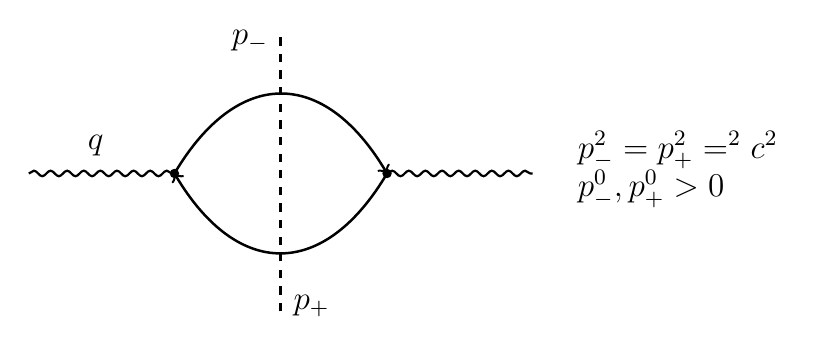
\begin{tikzpicture}[x=1cm,y=1cm,every node/.style={font=\large}]
 \coordinate (L) at (-3.2,0); \coordinate (a) at (-1.35,0);
 \coordinate (b) at (1.35,0); \coordinate (R) at (3.2,0);
 \draw[decorate,decoration={snake,amplitude=1.0pt,segment length=6pt},line width=.8pt] (L)--(a);
 \draw[decorate,decoration={snake,amplitude=1.0pt,segment length=6pt},line width=.8pt] (b)--(R);
 \draw[->,line width=.9pt] (a) .. controls (-.55,1.35) and (.55,1.35) .. (b);
 \draw[->,line width=.9pt] (b) .. controls (.55,-1.35) and (-.55,-1.35) .. (a);
 \fill (a) circle (1.7pt); \fill (b) circle (1.7pt);
 \draw[dashed,line width=1.05pt] (0,-1.75)--(0,1.75);
 \node at (-2.35,.35) {$q$};
 \node[anchor=south east,fill=white,inner sep=1pt] at (-.12,1.50) {$p_-$};
 \node[anchor=north west,fill=white,inner sep=1pt] at (.12,-1.50) {$p_+$};
 \node[align=left,right] at (3.65,.05) {$p_-^2=p_+^2=\me^2c^2$\\$p_-^0,p_+^0>0$};
\end{tikzpicture}

 \caption{QED 真空极化的 $e^-e^+$ 幺正性割线。虚线割线把费米子圈的两条内部线同时置于正能质量壳；其相空间阈值 $s=4\me^2c^2$ 产生 $\Pi_R(s)$ 的分支点。}
 \label{fig:qed-vacpol-cut-dp9}
\end{figure}

\begin{figure}[htbp]
 \centering
 
\includegraphics[width=0.82\textwidth]{qed_vacpol_dispersion_dp9.png}
 \caption{同一个重整化后的真空-极化函数的两种独立计算。实线直接数值积分 \eqnrefs{eq:Pi-spacelike-r12}；虚线只使用类时 $e^-e^+$ 谱权重 \eqnrefs{eq:qed-vacpol-spectral-weight-dp9} 代入色散关系 \eqnrefs{eq:qed-vacpol-dispersion-dp9}。两者重合验证了割线 $\to$ 色散的闭合链。}
 \label{fig:qed-vacpol-dispersion-dp9}
\end{figure}

这同时解释了自能与 LSZ 的关系，但需要区分三个容易混在一起的量：裸场与重整化场之间的场重整化常数 $Z_2$、某一给定场变量的精确二点函数极点留数，以及在壳方案中人为选成单位值的重整化传播子留数。它们彼此相关，却不是同一个定义。

先保留红外调节参数，使带电粒子的极点与连续谱割线暂时分离。对任意固定未来指向单位类时方向 $u^\mu$，沿 $p^\mu=\lambda u^\mu$ 定义正能投影后的标量逆传播子
\begin{equation*}
 d_+(\lambda)
 =\lambda-\me c-\sigma(\lambda),
\end{equation*}
其中 $\sigma(\lambda)$ 是上一节已经定义的正能投影自能本征值。若物理极点位于 $\lambda=\lambda_*$，则
\begin{equation*}
 d_+(\lambda_*)=0.
\end{equation*}
在简单极点条件 $d_+'(\lambda_*)\neq0$ 下，Laurent 展开给
\begin{equation}
 \boxed{
 Z_{\rm pole}
 =\frac{1}{d_+'(\lambda_*)}
 =\frac{1}{1-\sigma'(\lambda_*)}.}
 \label{eq:qed-pole-residue-selfenergy-dp9}
\end{equation}
这里 $Z_{\rm pole}$ 是“当前所用场变量的精确二点函数留数”，它才是谱表示中单粒子极点的权重。若采用一般重整化方案，LSZ 外腿因子由这个物理极点留数补偿；若采用在壳方案，则通过场强反项选择重整化场，使
\begin{equation*}
 Z_{\rm pole}^{(R)}=1.
\end{equation*}
这并不意味着裸场与重整化场之间的 $Z_2$ 等于 1。相反，$Z_2$ 正是反项参数的一部分，它被调节来使重整化后的传播子满足单位留数条件。因而“$Z_2$”“LSZ 极点留数”和“在壳归一化后的单位留数”必须在叙述中分开。

从谱论角度看，自能首先移动并重塑精确二点函数的单粒子极点；LSZ 随后取这个极点的留数并截去外腿传播子。圈自能对散射振幅的外腿影响因此通过极点位置与极点留数进入，而不是通过一个未定义的“$\partial/\partial\slashed p$”直接进入。

\begin{note}[无质量 QED 与 LSZ]
严格的无质量 QED 中，带电粒子总伴随任意软光子云；在非微扰谱意义上，由局域带电场产生的带电扇区具有红外粒子（infraparticle）结构，因此教科书式的孤立单粒子极点与 LSZ 约化需要红外调节参数、Bloch--Nordsieck/KLN 包容可观测量，或经过软光子缀饰的渐近态才能严格闭合。树级与固定阶在壳 QED 公式按受控的红外调节程序理解：先用调节器把单粒子极点与连续谱分开，从而分别定义受调节的极点权重 $Z_{\rm pole}^{(e)}$、场重整化常数 $Z_2$ 与散射振幅；随后在包容可观测量或缀饰态振幅中消去调节器依赖。这个红外问题不改变有质量电子的 Wigner 自旋分类，但会改变“局域带电场与精确渐近单粒子极点”之间最朴素的一一对应。
\end{note}

QED 一圈层与一般 QFT 的谱结构逐项对应：真空极化的 $e^-e^+$ 割线给出谱密度，色散关系由它重建类空区的实部；电子自能的割线决定连续谱阈值，而极点邻域导数首先决定当前场变量的 $Z_{\rm pole}^{(e)}$；在壳条件再据此固定场重整化常数 $Z_2$，LSZ 则用相应极点权重完成外腿归一化；交叉关系则把同一个截肢核连接到 Compton 散射、湮灭与对产生的不同物理区。新的圈图形状因子均应沿“极点与割线位置 $\to$ 不连续度 $\to$ 减法与重整化 $\to$ 物理投影”的顺序组织。


% -----------------------------------------------------------------------------
% Exact Ward--Takahashi identity from local U(1) covariance
% -----------------------------------------------------------------------------

局域 $U(1)$ 对称性不仅固定最小耦合顶角，也约束完整电子二点核与光子二点核。把精确一粒子不可约有效作用量记为 $\Gamma_{\rm 1PI}$，在经典背景四势 $A_\mu$ 中定义电子逆传播子
\begin{equation}
\boxed{
S_A^{-1}(x,y)
\equiv
\left.
\frac{\delta^2\Gamma_{\rm 1PI}}
{\delta\bar\psi(x)\,\delta\psi(y)}
\right|_{\psi=\bar\psi=0}.}
\label{eq:qed_background_inverse_propagator_definition}
\end{equation}
它是完整电子二点函数的逆核，并允许外部经典电磁背景任意强。采用
\[
A_\mu' = A_\mu-\partial_\mu\chi,
\qquad
U_\chi(x)=\exp\!\left(\frac{\ii \qe\chi(x)}{\hbar}\right),
\]
局域协变性要求
\begin{equation}
\boxed{
S_{A-\partial\chi}^{-1}(x,y)
=U_\chi(x)S_A^{-1}(x,y)U_\chi^{-1}(y).}
\label{eq:qed_inverse_propagator_gauge_covariance}
\end{equation}
这个关系不依赖微扰展开。规范固定只使光子二次核可逆，不改变费米子端点的局域相位变换律。

剥去电荷因子后，精确一粒子不可约电磁顶角定义为
\begin{equation}
\boxed{
\Gamma^\mu(x,y;z)
\equiv
-\frac{1}{\qe}
\left.
\frac{\delta S_A^{-1}(x,y)}{\delta A_\mu(z)}
\right|_{A=0}.}
\label{eq:qed_exact_vertex_functional_definition}
\end{equation}
树级时它退化为 $\Gamma^\mu=\gamma^\mu$。对\eqnrefs{eq:qed_inverse_propagator_gauge_covariance} 作无穷小规范变换，得到坐标空间 Ward--Takahashi 恒等式
\begin{equation}
\boxed{
\partial_\mu^z\Gamma^\mu(x,y;z)
=-\frac{\ii}{\hbar}
\bigl[\delta^{(4)}(z-x)-\delta^{(4)}(z-y)\bigr]
S^{-1}(x,y).}
\label{eq:qed_ward_takahashi_coordinate}
\end{equation}
两个接触项分别对应光子插入点与入射、出射费米子端点重合；相对负号来自两端相反的规范相位。

令入射电子动量为 $p^\mu$、出射电子动量为 $p^\mu+q^\mu$，按全文 $\exp(-\ii p\cdot x/\hbar)$ 的 Fourier 约定，\eqnrefs{eq:qed_ward_takahashi_coordinate} 等价于
\begin{equation}
\boxed{
q_\mu\Gamma^\mu(p+q,p)
=S^{-1}(p+q)-S^{-1}(p).}
\label{eq:qed_ward_takahashi_momentum}
\end{equation}
这里两边都是精确一粒子不可约核。任何固定圈阶都必须把 $S^{-1}$ 与 $\Gamma^\mu$ 按同一阶截断，才能保持这一约束。

在 $q\to0$ 且 $S^{-1}(p)$ 对外动量可微的区域，\eqnrefs{eq:qed_ward_takahashi_momentum} 给出
\begin{equation}
\boxed{
\Gamma^\mu(p,p)
=\frac{\partial S^{-1}(p)}{\partial p_\mu}.}
\label{eq:qed_ward_zero_momentum_vertex_derivative}
\end{equation}
因此电子波函数重整化与最小耦合顶角具有同一紫外乘法因子，
\begin{equation}
\boxed{Z_1=Z_2.}
\label{eq:qed_ward_z1_equals_z2}
\end{equation}
物理电荷归一化进一步固定在壳 Dirac 形状因子 $F_1(0)=1$；Pauli 形状因子 $F_2(0)$ 不由纵向 Ward 恒等式决定，必须由顶角的横向有限部分计算。

同一个局域对称性也约束光子二点的一粒子不可约量子修正。把真空极化张量定义为有效作用量中的二次核
\begin{equation}
\boxed{
\Gamma_{\Pi}^{(2)}[A]
=-\frac12\int\frac{\dd^4 q}{(2\pi\hbar)^4}\,
A_\mu(-q)\Pi^{\mu\nu}(q)A_\nu(q).}
\label{eq:qed-vacpol-quadratic-kernel-dp68}
\end{equation}
这里自由光子核和规范固定项不包含在 \(\Pi^{\mu\nu}\) 中。量子修正本身必须对 \(A_\mu\to A_\mu-\partial_\mu\chi\) 不变，因此
\begin{equation}
\boxed{q_\mu\Pi^{\mu\nu}(q)=0.}
\label{eq:qed_vacuum_polarization_transversality_from_1pi}
\end{equation}
在 Lorentz 不变真空中，横向性把它唯一约化为
\begin{equation}
\boxed{
\Pi^{\mu\nu}(q)
=\left(q^2\eta^{\mu\nu}-q^\mu q^\nu\right)\Pi(q^2).}
\label{eq:qed_vacuum_polarization_transverse_decomposition}
\end{equation}
因此真空极化的张量结构、$Z_1=Z_2$ 与外光子纵向极化解耦都是同一局域 $U(1)$ 约束的不同投影；具体圈积分只计算对称性未固定的标量函数和有限横向结构。

% -----------------------------------------------------------------------------
% One-loop QED: pole, charge and vertex renormalization as one physical chain
% -----------------------------------------------------------------------------

树级 QED 只有一个电子--光子局域顶角，但一圈以后出现三个彼此不同的一粒子不可约基本核：电子自能 \(\Sigma\)、光子真空极化 \(\Pi^{\mu\nu}\) 与电磁顶角修正 \(\Lambda^\mu\)。它们分别对应三类可测信息：电子传播子的单粒子极点确定物理质量与外腿归一化；长波长电磁交换确定低能电荷；在壳电磁顶角的额外张量结构确定磁矩等自旋响应。紫外发散出现在裸参数与这些可测定义之间的微扰关系中，质量、电荷和场强反项由相应的极点、留数与低能归一化条件固定。

对以特征物理动量 \(Q\) 探测、且没有大对数重求和的过程，固定一圈截断的两个控制量为
\begin{equation*}
\epsilon_{\rm 1L}\equiv\frac{\alpha(\mu)}{\pi},
\qquad
\epsilon_{\log}\equiv
\frac{\alpha(\mu)}{\pi}
\left|\ln\frac{Q^2}{\me^2c^2}\right|.
\end{equation*}
当 \(\epsilon_{\rm 1L}\ll1\) 且 \(\epsilon_{\log}\ll1\) 时，一圈截断把普通微扰误差控制在下一圈阶；若 \(\epsilon_{\log}\gtrsim1\)，固定圈阶中的大对数必须用重整化群或相应因子化结构重求和。Ward--Takahashi 恒等式本身不依赖这一截断。

电子二点函数先给出质量与外腿归一化。把重整化后的约化逆传播子写成
\begin{equation}
\boxed{
S_R^{-1}(p)
=\slashed p-\me c-\Sigma_R(p).}
\label{eq:qed-renormalized-electron-inverse-dp53}
\end{equation}
一般 Lorentz 协变自能同时含 $\slashed p$ 与标量两种 Dirac 结构，因此记为 $\Sigma_R(p)$。为定义单粒子极点沿质量壳法向的斜率，固定任意未来指向单位类时四矢量 $u^\mu$，满足 $u^2=1$，并沿同一方向写
\begin{equation*}
 p^\mu=\lambda u^\mu,
 \qquad [\lambda]={\rm kg\,m\,s^{-1}}.
\end{equation*}
正能投影算符为
\begin{equation*}
 P_+(u)\equiv\frac{\id_4+\slashed u}{2},
 \qquad P_+^2=P_+.
\end{equation*}
Lorentz 协变性保证自能在这个二维正能子空间内只留下一个标量本征值；定义
\begin{equation*}
 \sigma_R(\lambda)
 \equiv\frac12\Tr\!\left[P_+(u)\Sigma_R(\lambda u)\right],
 \qquad
 P_+\Sigma_R(\lambda u)P_+=\sigma_R(\lambda)P_+.
\end{equation*}
在壳点 $\lambda=\me c$，物理质量要求投影逆传播子在那里有零点，而单位留数要求这个零点对标量极点坐标 $\lambda$ 的一阶斜率等于自由值。两条条件严格写成
\begin{equation}
\boxed{
\sigma_R(\me c)=0,
\qquad
\left.\frac{\dd\sigma_R(\lambda)}{\dd\lambda}\right|_{\lambda=\me c}=0.}
\label{eq:qed-onshell-selfenergy-conditions-dp53}
\end{equation}
第一式固定质量反项，使极点仍在 $p^2=\me^2c^2$；第二式固定电子场强反项，使 LSZ 外腿抽出的正能单粒子极点具有单位留数。传统写法
$\Sigma_R(\slashed p)|_{\slashed p=\me c}=0$ 与
$\partial\Sigma_R/\partial\slashed p|_{\me c}=0$
就是这两个投影标量条件的简写；所谓“对 $\slashed p$ 求导”因此始终指这两个 Lorentz 标量系数的普通导数，而不是未定义的矩阵微分。

光子二点函数则固定电荷的低能归一化。真空极化的横向分解为
\begin{equation*}
\Pi^{\mu\nu}(q)
=(q^2\eta^{\mu\nu}-q^\mu q^\nu)\Pi(q^2),
\end{equation*}
在壳电荷方案中取
\begin{equation}
\boxed{\Pi_R(0)=0.}
\label{eq:qed-onshell-vacpol-condition-dp53}
\end{equation}
于是 \(q^2\to0\) 的长程 Coulomb/Thomson 极限直接使用实验测得的低能电荷；非零 \(q^2\) 时剩余的 \(\Pi_R(q^2)\) 才描述真空屏蔽随分辨尺度改变的物理效应。

电磁顶角把前两个问题连接起来。对在壳电子外腿，完整顶角由两个无量纲形状因子参数化：
\begin{equation*}
\bar u(p')\Gamma_R^\mu(p',p)u(p)
=\bar u(p')\left[
F_1(q^2)\gamma^\mu
+\frac{\ii\sigma^{\mu\nu}q_\nu}{2\me c}F_2(q^2)
\right]u(p).
\end{equation*}
低能电荷的定义要求
\begin{equation}
\boxed{F_1(0)=1,}
\label{eq:qed-F1-charge-normalization-dp53}
\end{equation}
而 \(F_2(0)\) 是 Ward--Takahashi 恒等式没有固定的有限横向结构；它给出反常磁矩
\begin{equation*}
a_e=\frac{g_{\rm mag}-2}{2}=F_2(0).
\end{equation*}
因此质量、低能电荷和反常磁矩分别由电子极点、零动量光子交换和横向顶角结构定义，对应传播子和顶角的三个独立可测信息。

精确 Ward--Takahashi 恒等\eqnrefs{eq:qed_ward_takahashi_momentum} 在一圈阶把电子自能与零动量转移顶角核直接联系起来。两者写为
\begin{equation}
\boxed{
\begin{aligned}
\Sigma_{\rm 1L}(p)
&=-\ii g_{\rm em}^2
\int_{\ell}^{(d)}
\frac{\gamma^\alpha\mathsf S_0(p-\ell)\gamma_\alpha}
{\ell^2+\ii0^+},\\
\Lambda_{\rm 1L}^{\mu}(p,p)
&=-\ii g_{\rm em}^2
\int_{\ell}^{(d)}
\frac{\gamma^\alpha\mathsf S_0(p-\ell)\gamma^\mu
\mathsf S_0(p-\ell)\gamma_\alpha}
{\ell^2+\ii0^+},
\end{aligned}}
\label{eq:qed-one-loop-selfenergy-vertex-kernels-dp68}
\end{equation}
其中 \(\mathsf S_0(k)\) 采用自由电子约化传播核及其既定极点处方。两式的区别只有内部电子线上是否插入一个零动量光子顶角。对同一内部传播核关于外动量求导，正好产生这个插入，因此
\begin{equation}
\boxed{
\Lambda_{\rm 1L}^{\mu}(p,p)
=-\frac{\partial\Sigma_{\rm 1L}(p)}{\partial p_\mu}.}
\label{eq:qed-one-loop-ward-kernel-dp53}
\end{equation}
这是一圈 Ward--Takahashi 恒等式的图级形式：电子自能对外动量的变化与零动量电磁顶角不是两个独立的紫外结构。

自能中乘在 \(\slashed p\) 前的紫外发散因此必须与最小耦合顶角的纵向紫外发散具有同一系数。若 \(Z_2\) 与 \(Z_1\) 分别表示电子场和顶角的重整化常数，则
\begin{equation}
\boxed{Z_1=Z_2.}
\label{eq:qed-Z1-Z2-dp53}
\end{equation}

电荷关系还需要比较同一个裸相互作用在裸场与重整化场中的两种写法。由
\(\psi_0=Z_2^{1/2}\psi_R\)、\(A_{0\mu}=Z_3^{1/2}A_{R\mu}\)，裸最小耦合项与以 \(Z_1\) 参数化的重整化顶角具有相同系数，当且仅当
\begin{equation}
\boxed{
q_0 Z_2 Z_3^{1/2}=q_R Z_1.}
\label{eq:qed-bare-renormalized-charge-match-dp68}
\end{equation}
代入\eqnrefs{eq:qed-Z1-Z2-dp53} 后，电子场因子约去，得到
\begin{equation}
\boxed{q_0=q_RZ_3^{-1/2}.}
\label{eq:qed-charge-Z3-dp53}
\end{equation}
所以阿贝尔电荷重整化的独立紫外信息只剩光子场因子 \(Z_3\)：电子外腿与纵向顶角的紫外重整化已经被局域 \(U(1)\) 对称性锁定为同一个量。

若把一圈 QED 看成对树级理论的第一次形变，可以用三个低能实验量给每个基本核定位。电子静止能确定精确传播子的极点位置 \(E=\me c^2\)，因此电子自能的常数部分不能独立成为新参数，而被质量反项重新吸收到物理质量定义中。低动量 Coulomb 或 Thomson 散射确定 \(q_R\)，因此真空极化在 \(q^2=0\) 的常数部分被条件 \(\Pi_R(0)=0\) 吸收；有限 \(Q\) 的偏离才表现为运行耦合。电子自旋在弱磁场中的进动则测量 \(g_{\rm mag}\)，其树级值 \(2\) 由 Dirac 方程给出，而一圈顶角的有限 Pauli 部分给出
\[
F_2(0)=\frac{\alpha}{2\pi}+O(\alpha^2).
\]
这三个观测量分别钉住极点、低能电荷和横向磁矩结构，因此一圈重整化的物理输入与三个一粒子不可约基本核的职责一一对应。

% -----------------------------------------------------------------------------
% One-loop QED vertex and Schwinger anomalous magnetic moment in strict SI
% -----------------------------------------------------------------------------

真空极化决定电荷随尺度的运行，电子自能决定极点质量与留数；在壳电磁顶角还包含一个不能由 Ward--Takahashi 恒等式单独固定的有限结构——Pauli 形状因子。它在零动量转移处直接给出电子反常磁矩。

\begin{figure}[htbp]
 \centering
 \begin{tikzpicture}[scale=.95,baseline=(current bounding box.center),
 fermion/.style={thick,postaction={decorate},decoration={markings,mark=at position .58 with {\arrow{Latex}}}},
 photon/.style={thick,decorate,decoration={snake,amplitude=1.2pt,segment length=6pt}}]
\coordinate (L) at (-2.2,0);
\coordinate (V1) at (-.8,0);
\coordinate (V2) at (0,0);
\coordinate (V3) at (.8,0);
\coordinate (R) at (2.2,0);
\draw[fermion] (L)--(V1)--(V2)--(V3)--(R);
\draw[photon] (V1) .. controls (-.55,1.55) and (.55,1.55) .. (V3);
\draw[photon] (V2)--(0,-1.8);
\node[above left] at (L) {$p$};
\node[above right] at (R) {$p'$};
\node[right] at (.08,-1.45) {$q=p'-p$};
\node[above] at (0,1.65) {$\ell$};
\end{tikzpicture}

 \caption{一圈 QED 顶角修正。外部电子四动量为 \(p^\mu,p'^\mu\)，外部光子注入 \(q^\mu=p'^\mu-p^\mu\)，内部光子圈动量为 \(\ell^\mu\)。所有四动量均采用 SI 物理四动量。}
 \label{fig:vertex-correction-r14}
\end{figure}

对在壳外腿，Gordon 恒等式把 Dirac 电流分成动量流与自旋磁矩两部分：
\begin{equation}
 \boxed{
 \bar u(p')\gamma^\mu u(p)
 =\frac1{2\me c}\bar u(p')
 \left[(p'+p)^\mu+\ii\sigma^{\mu\nu}q_\nu\right]u(p).}
 \label{eq:gordon-identity-r14}
\end{equation}
因此满足 Lorentz 协变性与电流守恒的在壳顶角可写成
\begin{equation}
 \boxed{
 \bar u(p')\Gamma^\mu(p',p)u(p)
 =\bar u(p')\left[
 F_1(q^2)\gamma^\mu
 +\frac{\ii\sigma^{\mu\nu}q_\nu}{2\me c}F_2(q^2)
 \right]u(p).}
 \label{eq:form-factor-definition-r14}
\end{equation}
其中 \(F_1(0)=1\) 由物理电荷归一化固定，\(F_2(0)\) 给出反常磁矩。

Feynman 规范中的一圈约化顶角修正从
\begin{equation}
 \Lambda_{\rm 1L}^\mu(p',p)
 =-\ii g_{\rm em}^2
 \int_{\ell}^{(d)}
 \frac{N^\mu(\ell)}{D_\gamma D'_eD_e}
 \label{eq:vertex-loop-start-r14}
\end{equation}
开始，其中三个传播子分母和自旋子分子分别为
\begin{equation}
\boxed{
\begin{aligned}
D_\gamma&=\ell^2+\ii0^+,\\
D'_e&=(p'-\ell)^2-\me^2c^2+\ii0^+,\\
D_e&=(p-\ell)^2-\me^2c^2+\ii0^+.
\end{aligned}}
\label{eq:vertex-propagator-denominators-dp75}
\end{equation}
\begin{equation}
\boxed{
N^\mu(\ell)=\gamma^\alpha
(\slashed p'-\slashed\ell+\me c)\gamma^\mu
(\slashed p-\slashed\ell+\me c)\gamma_\alpha.}
\label{eq:vertex-loop-numerator-dp75}
\end{equation}
三个分母依次对应内部光子以及外部光子顶角两侧的电子传播子；$N^\mu$ 是内部电子传播子的 Dirac 分子与三个 QED 顶角收缩后留下的自旋子空间矩阵。对\eqnrefs{eq:feynman-three-denominator-r14} 取
$A=D'_e$、$B=D_e$、$C=D_\gamma$，并利用在壳条件
$p^2=p'^2=\me^2c^2$。定义平移后的圈动量与参数化质量函数
\begin{equation}
\boxed{
L^\mu=\ell^\mu-xp'^\mu-yp^\mu,\qquad
\Delta_V(x,y,z;q^2)=(1-z)^2\me^2c^2-xyq^2,\qquad x+y+z=1,}
\label{eq:vertex-shift-delta-dp75}
\end{equation}
便有
\begin{equation}
\boxed{
\Lambda_{\rm 1L}^\mu
=-2\ii g_{\rm em}^2
\int_0^1\dd x\dd y\dd z\,
\delta(x+y+z-1)
\int_L^{(d)}
\frac{N^\mu(L;x,y,z)}{(L^2-\Delta_V+\ii0^+)^3}.}
\label{eq:vertex-parameterized-mother-dp75}
\end{equation}
\eqnrefs{eq:vertex-parameterized-mother-dp75} 是后续顶角计算的母积分；$\Delta_V$ 具有动量平方量纲，并把全部外部运动学集中在 Feynman 参数上。进一步的 Clifford 代数把该积分投影到\eqnrefs{eq:form-factor-definition-r14} 的两个独立 Lorentz 结构。对 Pauli 结构而言，参数化后的分子最终只留下
\begin{equation}
 \boxed{N_2(x,y,z)=4z(1-z)\me^2c^2,\qquad x+y+z=1.}
 \label{eq:vertex-pauli-numerator-r68}
\end{equation}


取零动量转移后，一圈 Pauli 形状因子得到 Schwinger 结果
\begin{equation}
 \boxed{
 F_2^{\rm 1L}(0)=\frac{\alpha}{2\pi}.}
 \label{eq:schwinger-F2-r14}
\end{equation}
Pauli 形状因子通过旋磁因子与实验磁矩相连。旋磁因子的物理定义为：对自旋 $1/2$ 粒子，$\mathbf S_{1/2}=\hbar\boldsymbol\sigma_{\rm P}/2$；把均匀弱磁场中的自旋能量写成
\begin{equation*}
 H_B=-\frac{g_{\rm mag}\qe}{2\me}\,\mathbf S_{1/2}\cdot\mathbf B,
\end{equation*}
其中无量纲数 $g_{\rm mag}$ 称为旋磁因子。树级 Dirac 方程给 $g_{\rm mag}=2$，而量子顶角修正会改变这个系数。这个 $g_{\rm mag}$ 与电磁顶角耦合常数 $g_e=\qe/\sqrt{\varepsilon_0\hbar c}$ 是不同物理量。

物理电荷归一化给出 \(F_1(0)=1\)。把偏离 Dirac 值 $2$ 的部分写成无量纲反常磁矩系数，则
\begin{equation}
 \boxed{
 a_\ee^{\rm anom}
 \equiv\frac{g_{\rm mag}-2}{2}
 =F_2(0),
 \qquad
 g_{\rm mag}=2[1+F_2(0)].}
 \label{eq:ae-form-factor-r68}
\end{equation}
结合\eqnrefs{eq:schwinger-F2-r14}，一圈阶有 \(a_\ee^{\rm anom}=\alpha/(2\pi)\)。普通一圈截断由 \(\alpha/\pi\ll1\) 控制；更高精度需要系统加入二圈及以上顶角、自能和真空极化贡献。

保留类空动量转移 \(Q^2\equiv-q^2>0\) 时，一圈结果可化为
\begin{equation}
 \boxed{
 \frac{F_2^{\rm 1L}(-Q^2)}{F_2^{\rm 1L}(0)}
 =\int_0^1\dd u_F\,
 \frac1{1+[Q/(\me c)]^2u_F(1-u_F)}.}
 \label{eq:F2-spacelike-ratio-r14}
\end{equation}
唯一的运动学比值是 \(Q/(\me c)\)：低动量极限恢复静态磁矩，高动量时电子有限 Compton 尺度使 Pauli 形状因子逐渐受抑。

\begin{figure}[htbp]
 \centering
 
\includegraphics[width=.76\linewidth]{qed_pauli_form_factor_r14.png}
 \caption{一圈 QED Pauli 形状因子的类空动量依赖。横轴为 \(Q/(\me c)\)，纵轴以 \(F_2(0)=\alpha/(2\pi)\) 归一化；曲线由\eqnrefs{eq:F2-spacelike-ratio-r14} 数值积分得到。}
 \label{fig:qed-pauli-form-factor-r14}
\end{figure}

% 高级 QED：真空极化势、软辐射与强平面波中的精确 Dirac 解

同一 QED 母理论在三个不同极限中呈现出三种可复用结构：真空极化修正静态光子传播子，软定理控制低能真实光子辐射，经典平面波背景则可以非微扰地吸收到 Dirac 方程的零阶解中。三者都沿用物理四动量、$q_{\mathrm e}=-e$ 和统一 Fourier 约定。

前面的圈图计算说明，虚粒子会修正传播子本身。要看这种修正在可观测空间势中留下什么痕迹，最直接的做法是先取静态极限：此时真空极化只改变 Coulomb 光子核的动量依赖，再通过三维 Fourier 变换回到位置空间。静态 Coulomb 核的一圈真空极化修正可写成
\begin{equation}
 \delta\widetilde V_U(\mathbf q)
 =\widetilde V_C(\mathbf q)\widehat\Pi(Q^2),
 \label{eq:Uehling-momentum-correction-r12}
\end{equation}
其中类空动量满足 $Q^2\equiv\mathbf q^2>0$。重整化真空极化的谱表示为
\begin{equation}
 \frac{\widehat\Pi(Q^2)}{Q^2}
 =\frac{\alpha}{3\pi}
 \int_{4m_{\mathrm e}^2c^2}^{\infty}\frac{\dd s}{s(s+Q^2)}
 \sqrt{1-\frac{4m_{\mathrm e}^2c^2}{s}}
 \left(1+\frac{2m_{\mathrm e}^2c^2}{s}\right).
 \label{eq:Pi-dispersion-explicit-r12}
\end{equation}
对三维动量作 Fourier 变换后得到
\begin{equation}
 \boxed{
 \delta V_U(r)
 =V_C(r)\frac{2\alpha}{3\pi}
 \int_1^\infty\dd t\,
 \ee^{-2rt/\lambda_C}
 \left(1+\frac1{2t^2}\right)
 \frac{\sqrt{t^2-1}}{t^2},
 \qquad
 \lambda_C\equiv\frac{\hbar}{m_{\mathrm e} c}.}
 \label{eq:Uehling-potential-SI-r12}
\end{equation}
积分核为正；对电子与正核的吸引 Coulomb 势 $V_C<0$，因此 $\delta V_U<0$。修正只在 $r\lesssim\lambda_C$ 的短距离显著，并以一圈参数 $\alpha/\pi$ 控制；更高圈从相对 $O(\alpha/\pi)$ 继续修正该一圈结果。

\begin{figure}[htbp]
 \centering
 \begin{tikzpicture}[scale=.82,baseline=(current bounding box.center),
 fermion/.style={thick,postaction={decorate},decoration={markings,mark=at position .58 with {\arrow{Latex}}}},
 photon/.style={thick,decorate,decoration={snake,amplitude=1.25pt,segment length=6pt}}]
\node[draw,circle,inner sep=2pt] (N) at (-3,0) {$Ze$};
\node[draw,circle,inner sep=2pt] (e) at (3,0) {$e^-$};
\draw[photon] (N)--(-1.0,0);
\draw[photon] (1.0,0)--(e);
\draw[fermion] (-1.0,0) arc (180:0:1.0 and .85);
\draw[fermion] (1.0,0) arc (0:-180:1.0 and .85);
\node[above] at (0,1.15){vacuum polarization};
\node[below] at (0,-1.15){$q^0=0$};
\end{tikzpicture}

 \caption{静态 Coulomb 交换中插入一次电子--正电子真空极化圈。重整化自能改变光子传播子的谱权重，三维 Fourier 变换后得到\eqnrefs{eq:Uehling-potential-SI-r12} 的 Uehling 势。}
 \label{fig:uehling-loop-r12}
\end{figure}

\begin{figure}[htbp]
 \centering
 
\includegraphics[width=.73\linewidth]{uehling_relative.png}
 \caption{点核 Uehling 修正的相对大小 $\delta V_U/V_C$ 随 $r/\lambda_C$ 的变化。曲线由\eqnrefs{eq:Uehling-potential-SI-r12} 数值积分得到。}
 \label{fig:uehling-relative-r12}
\end{figure}

真空极化处理的是虚光子圈对传播的修正；真实光子辐射则引入另一种尺度分离。当额外辐射光子的能量远小于硬散射的特征能量时，完整含光子振幅的领先项不再依赖硬子图的细节，而只由外部带电粒子的运动学决定。设电子在一个硬散射过程中从速度 $\boldsymbol\beta_{{\rm rel},i}$ 变到 $\boldsymbol\beta_{{\rm rel},f}$，并额外辐射方向为 $\mathbf n$、角频率为 $\omega$ 的软光子。若 $E_h$ 表示硬过程的最小特征能量，则
\begin{equation*}
 \epsilon_{\rm soft}^{(\gamma)}\equiv\frac{\hbar\omega}{E_h}\ll1
\end{equation*}
控制软展开。保留 $1/\omega$ 的领先外腿因子后，单光子辐射概率为
\begin{equation}
 \boxed{
 \dd P_{\rm soft}
 =\frac{\alpha}{4\pi^2}
 \frac{\dd\omega}{\omega}\,\dd\Omega
 \left|
 \frac{\boldsymbol\beta_{{\rm rel},f}^\perp}{1-\mathbf n\cdot\boldsymbol\beta_{{\rm rel},f}}
 -\frac{\boldsymbol\beta_{{\rm rel},i}^\perp}{1-\mathbf n\cdot\boldsymbol\beta_{{\rm rel},i}}
 \right|^2.}
 \label{eq:soft-photon-probability-r12}
\end{equation}
相对于领先软项，有限光子能量修正由 $\epsilon_{\rm soft}^{(\gamma)}$ 控制；当它不再远小于一时，必须恢复完整含光子过程的矩阵元。多软光子与虚软修正的包容处理由一般红外母式给出，不能把\eqnrefs{eq:soft-photon-probability-r12} 单独积分到 $\omega=0$。

\begin{figure}[htbp]
 \centering
 \begin{tikzpicture}[scale=.78, baseline=(current bounding box.center), hard/.style={draw,rounded corners,minimum width=1.0cm,minimum height=.9cm,fill=black!4}]
\begin{scope}[xshift=-4cm]
\node[hard] (H) at (0,0) {$\mathcal H$};
\draw[fermion] (-2.2,0)--(-.6,0);\draw[fermion] (.6,0)--(2.2,0);
\coordinate (v) at (1.25,0);
\draw[photon] (v)--(2.1,1.35);
\node[below] at (1.45,-.4){outgoing};
\end{scope}
\node at (0,0){$+$};
\begin{scope}[xshift=4cm]
\node[hard] (H) at (0,0) {$\mathcal H$};
\draw[fermion] (-2.2,0)--(-.6,0);\draw[fermion] (.6,0)--(2.2,0);
\coordinate (v) at (-1.25,0);
\draw[photon] (v)--(-2.1,1.35);
\node[below] at (-1.45,-.4){incoming};
\end{scope}
\end{tikzpicture}

 \caption{软光子附着在同一条外部电子线的出射与入射两种位置。领先 $1/\omega$ 奇异性只依赖外腿四动量，因此从任意硬子图因子化。}
 \label{fig:soft-brems-r12}
\end{figure}

\begin{figure}[htbp]
 \centering
 
\includegraphics[width=.76\linewidth]{soft_brems_angular.png}
 \caption{软光子辐射的角向几何因子。取入射与出射电子速率均为 $\beta_{\rm rel}=0.8$，电子偏转角为 $25^\circ$；曲线只计算\eqnrefs{eq:soft-photon-probability-r12} 方括号中的几何因子，因此不对应特定实验装置。}
 \label{fig:soft-brems-angular-r12}
\end{figure}

软展开仍把电磁场作为量子辐射处理；若外加光场具有很高占据数，而且其经典波形已知，更自然的组织方式是把这部分场直接并入零阶 Dirac 方程，而不是把它逐光子展开。平面波背景是少数能够把这一步精确完成的时空依赖场。令经典四势只依赖无量纲相位
\begin{equation*}
 \phi\equiv\kappa\cdot x,
 \qquad
 \kappa^2=0,
 \qquad
 \kappa\cdot A(\phi)=0,
\end{equation*}
其中 $\kappa^\mu$ 是逆长度量纲的平面波四波矢。背景中的 Dirac 方程为
\begin{equation}
 [\ii\hbar\slashed\partial-q_{\mathrm e}\slashed A(\phi)-m_{\mathrm e} c]\psi(x)=0.
 \label{eq:Volkov-Dirac-r12}
\end{equation}
取自由在壳四动量 $p^\mu$ 和自旋子 $u_s(p)$，并定义
\begin{align*}
 R_p(\phi)
 &\equiv
 1+\frac{q_{\mathrm e}}{2p\cdot\kappa}
 \slashed\kappa\slashed A(\phi),\\
 F_p(\phi)
 &\equiv
 \frac{q_{\mathrm e} p\cdot A(\phi)}{p\cdot\kappa}
 -\frac{q_{\mathrm e}^2A^2(\phi)}{2p\cdot\kappa},\\
 S_p(x)
 &\equiv p\cdot x+\int^{\phi}\dd\varphi\,F_p(\varphi).
\end{align*}
$R_p$ 无量纲，而 $F_p$ 与 $S_p$ 具有作用量量纲，因此 $S_p/\hbar$ 无量纲。任意强度平面波中的精确 Volkov 解为
\begin{equation}
 \boxed{
 \psi_{p,s}^{\rm V}(x)
 =R_p(\phi)u_s(p)
 \exp\left[-\frac{\ii}{\hbar}S_p(x)\right].}
 \label{eq:Volkov-solution-r12}
\end{equation}
它不是弱场展开；背景强度全部保留在 $R_p$ 与 $S_p$ 中。

若背景对 $\phi$ 周期，并选取 $\langle A\rangle_\phi=0$ 的规范，周期平均相位定义准动量
\begin{equation}
 \boxed{
 \bar p^\mu
 =p^\mu
 -\frac{q_{\mathrm e}^2\langle A^2\rangle_\phi}{2p\cdot\kappa}\kappa^\mu,
 \qquad
 \bar p^2=m_{\mathrm e}^2c^2-q_{\mathrm e}^2\langle A^2\rangle_\phi.}
 \label{eq:volkov-quasimomentum-dp43}
\end{equation}
以峰值矢势定义无量纲强度
\begin{equation*}
 a_0\equiv\frac{|q_{\mathrm e}|A_0}{m_{\mathrm e} c}.
\end{equation*}
圆偏振与线偏振分别满足
\begin{equation}
 \boxed{
 m_*^{\rm circ}=m_{\mathrm e}\sqrt{1+a_0^2},
 \qquad
 m_*^{\rm lin}=m_{\mathrm e}\sqrt{1+\frac{a_0^2}{2}}.}
 \label{eq:volkov-effective-mass-dp43}
\end{equation}
只有进一步取 $a_0\ll1$ 时，才可把这些精确平面波结果重新展开成普通弱场多光子微扰级数。

\begin{figure}[htbp]
 \centering
 \begin{tikzpicture}[scale=.82,baseline=(current bounding box.center),
 fermion/.style={very thick,postaction={decorate},decoration={markings,mark=at position .6 with {\arrow{Latex}}}},
 wave/.style={thick,decorate,decoration={snake,amplitude=2.0pt,segment length=8pt}}]
\draw[fermion] (-3.2,-.8) .. controls (-1.2,-.2) and (1.2,.2) .. (3.2,.8);
\foreach \y in {-1.2,-.6,0,.6,1.2}{\draw[wave] (-2.8,\y+1.0)--(2.8,\y-1.0);}
% Labels are intentionally outside the dense wave bundle.
\node[anchor=east,fill=white,inner sep=1.2pt] at (-3.0,-.92){$p^\mu$};
\node[anchor=west,fill=white,inner sep=1.2pt] at (3.0,.92){$\bar p^\mu$};
\node[anchor=south,fill=white,inner sep=2pt] at (0,2.12){classical background $A^\mu(\kappa\!\cdot\! x)$};
\end{tikzpicture}

 \caption{Volkov 问题的物理结构：电子在任意强度经典平面波背景中传播。波线表示外加经典背景，不是内部光子传播子。}
 \label{fig:volkov-plane-wave-r12}
\end{figure}

\begin{figure}[htbp]
 \centering
 
\includegraphics[width=.72\linewidth]{volkov_effective_mass.png}
 \caption{Volkov 有效质量随归一化矢势 $a_0$ 的变化。线偏振与圆偏振的差异来自周期平均 $\langle A^2\rangle_\phi$ 不同；曲线直接使用\eqnrefs{eq:volkov-effective-mass-dp43}。}
 \label{fig:volkov-effective-mass-r12}
\end{figure}

Uehling 势、软制动辐射与 Volkov 解分别对应 QED 的三个受控读取：一圈传播子谱修正、低能真实光子的外腿因子化，以及强经典平面波被精确吸收到零阶 Dirac 算符。它们共享同一作用量和 SI 约定，差异只在所选择的尺度层级与外场处理方式。


带电粒子散射会改变其长程 Coulomb 场，因此任意低频电磁辐射与硬散射态不可完全分离。探测器只能以有限能量分辨率区分辐射：若未分辨光子的总能量低于阈值 $\Delta E_{\rm det}$，实验可观测量必须把这些末态与无辐射硬末态共同计入。红外有限性因此是包容测量定义与 QED 幺正性的共同结果，而不是单张图的性质。

带电粒子的速度发生改变时，其长程电磁场必须重新调整，这一调整包含频率可以任意低的辐射。严格要求末态“没有任何光子”会把实验上不可分辨的低频辐射排除在外，从而产生红外发散。有限的 $\Delta E_{\rm det}$ 把所有不可分辨软光子态组成同一个实验结果。


设硬过程的约化振幅为 $\mathcal M_0$，外部带电腿编号 $i=1,\ldots,N$。第 $i$ 条腿的电荷写成 $Q_i e$，其中 $Q_i$ 是带符号的无量纲电荷数；出射腿取 $\sigma_i^{\rm io}=+1$，入射腿取 $\sigma_i^{\rm io}=-1$。再发射一条物理四动量为
$k^\mu=(\hbar\omega/c,\hbar\mathbf k)$、横向偏振为 $\varepsilon_\lambda^\mu(k)$ 的软光子。令 $p_{\rm hard}$ 表示硬过程的典型物理动量尺度。当
\[
 \epsilon_{\rm soft}\equiv
 \max_i\frac{|p_i\!\cdot k|}{p_{\rm hard}^2}\ll1
\]
时，内部离壳传播子对 $k\to0$ 保持有限，只有外部在壳带电腿产生 $1/(p_i\!\cdot k)$ 极点。以一条出射费米子腿为例，软光子附着在该腿上的精确外线因子可写成
\begin{equation}
 \boxed{
 \mathcal L_{i,\lambda}^{\rm out}(k)
 =g_{\rm em}Q_i\,
 \bar u(p_i)\slashed\varepsilon_\lambda^*(k)
 \frac{\slashed p_i+\slashed k+m_ic}
 {(p_i+k)^2-m_i^2c^2+\ii0^+}.}
 \label{eq:soft-external-leg-kernel-dp68}
\end{equation}
它仍保留完整的 $k$ 依赖；软近似只在下一步展开这个因子。领先软振幅因此因子化为
\begin{equation}
 \boxed{
 \mathcal M_{1\gamma}^{\rm soft}(k,\lambda)
 =S_\lambda(k)\,\mathcal M_0+\order(\omega^0),
 \qquad
 S_\lambda(k)
 =g_{\rm em}\sum_{i=1}^{N}
 \sigma_i^{\rm io}Q_i
 \frac{p_i\!\cdot\varepsilon_\lambda^*(k)}{p_i\!\cdot k}.}
 \label{eq:weinberg-soft-photon-factor-dp10}
\end{equation}
这里 $g_{\rm em}=\sqrt{4\pi\alpha}$ 无量纲。由于增加一条外部光子会改变约化振幅的质量维数，$S_\lambda$ 本身带相应的逆动量量纲；与光子相空间组合后的辐射概率才是无量纲量。硬过程的全部内部动力学只保留在 $\mathcal M_0$ 中。电荷守恒
$\sum_i\sigma_i^{\rm io}Q_i=0$ 使 $\varepsilon^\mu\to\varepsilon^\mu+\zeta k^\mu$ 不改变\eqnrefs{eq:weinberg-soft-photon-factor-dp10}，因此领先软因子自身满足规范不变性。

实软辐射的概率由\eqnrefs{eq:weinberg-soft-photon-factor-dp10} 与一光子 Lorentz 不变相空间共同决定。记 $\mathbf n$ 为光子传播方向，$\boldsymbol\beta_i=c\mathbf p_i/E_i$，并定义相对于 $\mathbf n$ 的横向速度
$\boldsymbol\beta_i^\perp=\boldsymbol\beta_i-\mathbf n(\mathbf n\!\cdot\boldsymbol\beta_i)$。用红外能量调节参数 $\lambda_{\rm IR}>0$ 暂时截断 $\hbar\omega\to0$ 区域，未分辨真实软辐射的无量纲积分为
\begin{equation}
 \boxed{
 \mathcal R(\lambda_{\rm IR},\Delta E_{\rm det})
 =\frac{\alpha}{4\pi^2}
 \int_{\lambda_{\rm IR}/\hbar}^{\Delta E_{\rm det}/\hbar}
 \frac{\dd\omega}{\omega}
 \int\dd\Omega\,
 \left|
 \sum_i\sigma_i^{\rm io}Q_i
 \frac{\boldsymbol\beta_i^\perp}
 {1-\mathbf n\!\cdot\boldsymbol\beta_i}
 \right|^2.}
 \label{eq:soft-radiator-definition-dp10}
\end{equation}
频率积分显式含 $\ln(\Delta E_{\rm det}/\lambda_{\rm IR})$，因此“硬过程加一条真实软光子”的概率单独并没有 $\lambda_{\rm IR}\to0$ 极限。

同一微扰阶的虚软光子修正具有完全相同的外腿软因子核。把虚光子割到质量壳上会产生与\eqnrefs{eq:soft-radiator-definition-dp10} 相同的一光子相空间，而幺正性固定其概率流方向为相反号。红外奇异部分满足
\begin{equation}
 \boxed{
 2\Re\frac{\delta_{\rm virt}^{\rm soft}\mathcal M_0}{\mathcal M_0}
 =-\mathcal R(\lambda_{\rm IR},\Delta E_{\rm det})
 +C_{\rm IR\,finite},}
 \label{eq:virtual-real-ir-relation-dp10}
\end{equation}
其中 $C_{\rm IR\,finite}$ 在 $\lambda_{\rm IR}\to0$ 时有限。于是包含未分辨真实软辐射的包容概率满足
\begin{equation}
 \boxed{
 \lim_{\lambda_{\rm IR}\to0}
 P_{\rm incl}(\Delta E_{\rm det})<\infty.}
 \label{eq:bloch-nordsieck-cancellation-dp10}
\end{equation}
调节参数从物理预测中消失，但 $\Delta E_{\rm det}$ 保留下来，因为它属于实验测量定义。

领先软极限中，多条未分辨光子从同一个外腿电流独立因子化。若每条光子都位于同一软窗口，并忽略总软能量约束产生的次领先相关，则 $n$ 条不可分辨软光子的独立发射权重满足
\begin{equation}
 \boxed{
 P_n^{\rm soft}=\frac{\mathcal R^n}{n!}P_0^{\rm soft}.}
 \label{eq:soft-independent-n-emission-dp68}
\end{equation}
幺正性再固定零光子概率与全部 $n$ 光子概率的共同归一化：
\begin{equation}
 \boxed{
 P_0^{\rm soft}=\ee^{-\mathcal R},
 \qquad
 P_n^{\rm soft}
 =\ee^{-\mathcal R}\frac{\mathcal R^n}{n!}.}
 \label{eq:bloch-nordsieck-exponentiation-dp10}
\end{equation}
这就是 Bloch--Nordsieck 指数化：虚软修正降低严格无辐射通道的概率，真实软发射把同一概率重新分配到实验上退化的多光子扇区。

有质量 QED 中，电子质量切断严格共线发散；当 $m_{\mathrm e} c^2$ 远小于硬能标时，共线区仍产生大的质量对数。若电子能量为 $E$、光子与电子夹角为 $\theta$，则
\begin{equation}
 \boxed{
 p\!\cdot k
 =\frac{E\hbar\omega}{c^2}
 \left(1-\beta_{\rm rel}\cos\theta\right).}
 \label{eq:soft-collinear-dot-exact-dp68}
\end{equation}
在 $\theta\ll1$ 且 $m_{\mathrm e} c^2/E\ll1$ 时，才进一步展开为
\begin{equation}
 \boxed{
 p\!\cdot k
 \simeq
 \frac{E\hbar\omega}{2c^2}
 \left(\theta^2+\frac{m_{\mathrm e}^2c^4}{E^2}\right).}
 \label{eq:soft-collinear-denominator-dp10}
\end{equation}
从而软极限与共线极限可以重叠。Kinoshita--Lee--Nauenberg 定理要求对给定实验分辨率下所有退化的初态和末态作适当求和或平均；Bloch--Nordsieck 对未分辨末态软光子的求和只是其中一个特例。

\begin{note}[带电渐近态与 LSZ]
严格无质量光子 QED 中，带电渐近态携带无限软光子云，局域裸电子场与孤立单粒子极点之间的朴素对应会被红外粒子（infraparticle）结构改变。固定阶散射计算可先引入红外调节参数或使用适当缀饰态，在形成包容可观测量以后再取去调节极限。由此，LSZ 的孤立极点假设与严格红外极限的带电渐近态不发生逻辑冲突。
\end{note}

外部在壳极点产生普适软因子，光子相空间把 $1/\omega$ 振幅转化为红外对数，虚软程函核由幺正性给出相反的红外对数，包容求和消去调节参数，多软光子概率再由同一幺正性结构指数化。QCD 中对应的软与共线因子化保留这条动力学链，但电荷数被不对易的颜色生成元取代。


% Detailed proofs for 04qed-ward-takahashi
\begin{derivation}[从\eqnrefs{eq:qed_inverse_propagator_gauge_covariance}到\eqnrefs{eq:qed_ward_takahashi_coordinate}]

正文\eqnrefs{eq:qed_inverse_propagator_gauge_covariance} 给出背景场变化时精确电子逆传播子的端点协变性。对任意无穷小规范函数 $\chi$ 比较等式两侧的一阶变化，便能把这种端点相位约束转写成顶角的坐标空间散度关系。

左端对背景场作泛函展开，
\begin{align*}
 S_{-\partial\chi}^{-1}(x,y)
 &=S_0^{-1}(x,y)
 -\int\dd^4 z\,
 \left.\frac{\delta S_A^{-1}(x,y)}{\delta A_\mu(z)}\right|_0
 \partial_\mu\chi(z)+O(\chi^2)\\
 &=S_0^{-1}(x,y)
 +\qe\int\dd^4 z\,\Gamma^\mu(x,y;z)\partial_\mu\chi(z)+O(\chi^2)\\
 &=S_0^{-1}(x,y)
 -\qe\int\dd^4 z\,[\partial_\mu^z\Gamma^\mu(x,y;z)]\chi(z)+O(\chi^2).
\end{align*}
右端的两个端点相位展开为
\begin{align*}
 U_\chi(x)S_0^{-1}(x,y)U_\chi^{-1}(y)
 &=S_0^{-1}(x,y)
 +\frac{\ii\qe}{\hbar}[\chi(x)-\chi(y)]S_0^{-1}(x,y)+O(\chi^2).
\end{align*}
两个端点值分别可写成
\begin{equation*}
 \chi(x)=\int\dd^4z\,\delta^{(4)}(z-x)\chi(z),
 \qquad
 \chi(y)=\int\dd^4z\,\delta^{(4)}(z-y)\chi(z).
\end{equation*}
所以右端一阶变化等于
\begin{equation*}
 \frac{\ii\qe}{\hbar}\int\dd^4z\,
 \bigl[\delta^{(4)}(z-x)-\delta^{(4)}(z-y)\bigr]
 S_0^{-1}(x,y)\chi(z).
\end{equation*}
与左端
\begin{equation*}
 -\qe\int\dd^4z\,
 [\partial_\mu^z\Gamma^\mu(x,y;z)]\chi(z)
\end{equation*}
相等。由于 $\chi(z)$ 是任意光滑测试函数，两个分布作用在任意测试函数上的积分都相等，只能有
\begin{equation*}
 \partial_\mu^z\Gamma^\mu(x,y;z)
 =-\frac{\ii}{\hbar}
 \bigl[\delta^{(4)}(z-x)-\delta^{(4)}(z-y)\bigr]
 S_0^{-1}(x,y),
\end{equation*}
即正文\eqnrefs{eq:qed_ward_takahashi_coordinate}。这里的两个 $\delta$ 接触项正是端点相位 $\chi(x)-\chi(y)$ 的分布表示：一个支撑在电子线的入射端点，另一个支撑在出射端点，二者符号相反。
\end{derivation}

\begin{derivation}[从\eqnrefs{eq:qed_ward_takahashi_coordinate}到\eqnrefs{eq:qed_ward_zero_momentum_vertex_derivative}]
按正文固定的 $\exp(-\ii p\cdot x/\hbar)$ 约定，把平移不变的逆传播子和三点顶角展开为
\begin{align*}
S^{-1}(x,y)
&=\int_p
 \ee^{-\ii p\cdot x/\hbar}
 \ee^{+\ii p\cdot y/\hbar}S^{-1}(p),\\
\Gamma^\mu(x,y;z)
&=\int_p\!\int_q
 \ee^{-\ii(p+q)\cdot x/\hbar}
 \ee^{+\ii p\cdot y/\hbar}
 \ee^{+\ii q\cdot z/\hbar}
 \Gamma^\mu(p+q,p),
\end{align*}
其中 $\int_p\equiv\int \dd^4 p/(2\pi\hbar)^4$。正文\eqnrefs{eq:qed_ward_takahashi_coordinate} 左边的 $z$ 导数只作用在最后一个 Fourier 相位上，因此
\begin{align*}
\partial_\mu^z\Gamma^\mu(x,y;z)
&=\int_p\!\int_q
 \ee^{-\ii(p+q)\cdot x/\hbar}
 \ee^{+\ii p\cdot y/\hbar}
 \ee^{+\ii q\cdot z/\hbar}
 \frac{\ii q_\mu}{\hbar}
 \Gamma^\mu(p+q,p).
\end{align*}
两个接触项分别使用
\begin{equation*}
\delta^{(4)}(z-x)=\int_q\ee^{+\ii q\cdot(z-x)/\hbar},
\qquad
\delta^{(4)}(z-y)=\int_q\ee^{+\ii q\cdot(z-y)/\hbar}.
\end{equation*}
第一项给
\begin{align*}
\delta^{(4)}(z-x)S^{-1}(x,y)
=\int_p\!\int_q
 \ee^{-\ii(p+q)\cdot x/\hbar}
 \ee^{+\ii p\cdot y/\hbar}
 \ee^{+\ii q\cdot z/\hbar}S^{-1}(p),
\end{align*}
而第二项把逆传播子的积分变量改写成 $p+q$ 后成为
\begin{align*}
\delta^{(4)}(z-y)S^{-1}(x,y)
=\int_p\!\int_q
 \ee^{-\ii(p+q)\cdot x/\hbar}
 \ee^{+\ii p\cdot y/\hbar}
 \ee^{+\ii q\cdot z/\hbar}S^{-1}(p+q).
\end{align*}
于是坐标空间恒等式两侧具有同一个 Fourier 核。比较系数，
\begin{equation*}
\frac{\ii}{\hbar}q_\mu\Gamma^\mu(p+q,p)
=-\frac{\ii}{\hbar}\left[S^{-1}(p)-S^{-1}(p+q)\right],
\end{equation*}
约去共同的 $\ii/\hbar$，得到正文\eqnrefs{eq:qed_ward_takahashi_momentum}：
\begin{equation*}
 q_\mu\Gamma^\mu(p+q,p)
 =S^{-1}(p+q)-S^{-1}(p).
\end{equation*}

再取 $q\to0$，并使用正文已经说明的可微条件。右边作 Taylor 展开：
\begin{equation*}
 S^{-1}(p+q)-S^{-1}(p)
 =q_\mu\frac{\partial S^{-1}(p)}{\partial p_\mu}+O(q^2).
\end{equation*}
左边的精确顶角在同一点展开为
\begin{equation*}
 q_\mu\Gamma^\mu(p+q,p)
 =q_\mu\Gamma^\mu(p,p)+O(q^2).
\end{equation*}
两边对任意足够小的四矢量 $q_\mu$ 都相等，因此比较每个独立的一阶系数得到
\begin{equation*}
 \Gamma^\mu(p,p)=\frac{\partial S^{-1}(p)}{\partial p_\mu},
\end{equation*}
即正文\eqnrefs{eq:qed_ward_zero_momentum_vertex_derivative}。
\end{derivation}

\begin{derivation}[从\eqnrefs{eq:qed_ward_zero_momentum_vertex_derivative}到\eqnrefs{eq:qed_ward_z1_equals_z2}]

完整 1PI 顶角与完整电子逆传播子满足
\[
q_\mu\Gamma_B^\mu(p+q,p)
=
S_B^{-1}(p+q)-S_B^{-1}(p).
\]
令 \(q\to0\)，对 \(q_\mu\) 作一阶展开即得正文
\eqnrefs{eq:qed_ward_zero_momentum_vertex_derivative}：
\[
\Gamma_B^\mu(p,p)
=
\frac{\partial S_B^{-1}(p)}{\partial p_\mu}.
\]
这个关系作用在完整裸量上，因此任何紫外发散都必须在等式两边以相同方式出现。

要从这个恒等式抽取重整化常数，最干净的做法是只投影它的局域紫外发散部分，而不把方案依赖的有限项混进来。由表面发散度和 Lorentz 协变性，电子二点 1PI 核的局域紫外发散最多具有
\begin{equation*}
 \bigl[S_B^{-1}(p)\bigr]_{\rm UV,loc}
 =A_{\rm UV}\,\slashed p
 +B_{\rm UV}\,m_Rc,
\end{equation*}
其中 $A_{\rm UV},B_{\rm UV}$ 可以含 $1/\epsilon$ 极点，但不再依赖外动量；更高次的 $p$ 幂会对应不可重整化的局域算符。对 $p_\mu$ 求导后，质量型发散自动消失：
\begin{equation*}
 \frac{\partial}{\partial p_\mu}
 \bigl[S_B^{-1}(p)\bigr]_{\rm UV,loc}
 =A_{\rm UV}\gamma^\mu.
\end{equation*}

另一方面，零光子动量处的三点 1PI 顶角在 QED 中只有同维数的局域 Dirac 结构
\begin{equation*}
 \bigl[\Gamma_B^\mu(p,p)\bigr]_{\rm UV,loc}
 =C_{\rm UV}\gamma^\mu.
\end{equation*}
把这两个局域发散部分代入精确零动量 Ward--Takahashi 恒等式
\begin{equation*}
 \Gamma_B^\mu(p,p)
 =\frac{\partial S_B^{-1}(p)}{\partial p_\mu},
\end{equation*}
于是恒等式在唯一允许的局域基矢 $\gamma^\mu$ 上给出：
\begin{equation*}
 C_{\rm UV}\gamma^\mu=A_{\rm UV}\gamma^\mu
 \quad\Longrightarrow\quad
 C_{\rm UV}=A_{\rm UV}.
\end{equation*}

现在把反项写成
\begin{equation*}
 \delta_2\,\bar\psi_R\,\ii\hbar c\slashed\partial\psi_R,
 \qquad
 -\delta_1 q_Rc\,\bar\psi_R\gamma^\mu\psi_R A_{\mu,R},
 \qquad
 \delta_i\equiv Z_i-1.
\end{equation*}
重整化条件要求反项逐个抵消上述局域紫外系数，因此在同一符号约定下
\begin{equation*}
 \delta_2=-A_{\rm UV},
 \qquad
 \delta_1=-C_{\rm UV}.
\end{equation*}
由 $C_{\rm UV}=A_{\rm UV}$ 立即有
\begin{equation*}
 \delta_1=\delta_2,
 \qquad
 \boxed{Z_1=Z_2.}
\end{equation*}
质量反项不参与这一投影，因为 $\partial(m_Rc)/\partial p_\mu=0$；有限顶角与有限自能导数则继续由同一个 Ward--Takahashi 恒等式彼此约束。

因此，在保持局域 $U(1)$ Ward 恒等式的调节与重整化方案中，$Z_1=Z_2$ 是全阶约束。结合裸电荷与重整化电荷的关系，独立的电荷重整化信息只剩光子场因子 $Z_3$。
\end{derivation}

\begin{derivation}[从\eqnrefs{eq:qed-vacpol-quadratic-kernel-dp68}到\eqnrefs{eq:qed_vacuum_polarization_transversality_from_1pi}]

正文\eqnrefs{eq:qed-vacpol-quadratic-kernel-dp68} 把真空极化定义成光子有效作用量中的量子二次核。对它施加无穷小规范变换后，任意规范函数 \(\chi(q)\) 前的系数必须消失；这会直接限制 \(\Pi^{\mu\nu}\) 的纵向分量。

Fourier 空间的无穷小变换为
\begin{equation*}
\delta A_\mu(q)=-\frac{\ii}{\hbar}q_\mu\chi(q).
\end{equation*}
对正文\eqnrefs{eq:qed-vacpol-quadratic-kernel-dp68} 作一阶变分。二次核满足 $\Pi^{\mu\nu}(q)=\Pi^{\nu\mu}(-q)$；第二项作 $q\mapsto-q$ 后可与第一项合并，严格得到
\begin{equation*}
\delta\Gamma_{\Pi}^{(2)}
=-\frac{\ii}{\hbar}
\int\frac{\dd^4 q}{(2\pi\hbar)^4}\,
\chi(-q)q_\mu\Pi^{\mu\nu}(q)A_\nu(q).
\end{equation*}
规范函数 \(\chi\) 与测试场 \(A_\nu\) 可以独立选择，而量子有效作用量必须对任意 \(\chi\) 保持不变，因此只有
\begin{equation*}
q_\mu\Pi^{\mu\nu}(q)=0
\end{equation*}
才能使变分恒为零，这就是正文\eqnrefs{eq:qed_vacuum_polarization_transversality_from_1pi}。
\end{derivation}

% Detailed proofs for 04qed-one-loop-ward-renormalization

\begin{derivation}[从\eqnrefs{eq:qed-renormalized-electron-inverse-dp53}到\eqnrefs{eq:qed-onshell-selfenergy-conditions-dp53}]
正文把极点问题化成一个真正的一维标量问题。固定未来指向单位类时四矢量 $u^\mu$，令
\begin{equation*}
 p^\mu=\lambda u^\mu,
 \qquad
 P_+(u)=\frac{\id_4+\slashed u}{2}.
\end{equation*}
因为 $u^2=1$，Clifford 关系给
\begin{equation*}
 (\slashed u)^2=\id_4,
 \qquad
 P_+\slashed u=\slashed uP_+=P_+.
\end{equation*}
因此自由逆传播子投影到正能子空间后只有一个标量因子：
\begin{align*}
 P_+(\slashed p-\me c)P_+
 &=P_+(\lambda\slashed u-\me c)P_+\\
 &=(\lambda-\me c)P_+.
\end{align*}

一般 Lorentz 协变、宇称偶的电子自能可写成
\begin{equation*}
 \Sigma_R(p)=A_R(p^2)\slashed p+B_R(p^2)\me c,
\end{equation*}
其中 $A_R,B_R$ 是标量函数。沿 $p=\lambda u$ 投影：
\begin{align*}
 P_+\Sigma_R(\lambda u)P_+
 &=\left[\lambda A_R(\lambda^2)+\me c\,B_R(\lambda^2)\right]P_+.
\end{align*}
这说明正文定义的
\begin{equation*}
 \sigma_R(\lambda)
 =\frac12\Tr\!\left[P_+\Sigma_R(\lambda u)\right]
\end{equation*}
确实就是正能二维子空间上的自能本征值，因为 $\Tr P_+=2$。于是完整逆传播子满足
\begin{equation*}
 P_+S_R^{-1}(\lambda u)P_+
 =d_+(\lambda)P_+,
\end{equation*}
其中
\begin{equation*}
 d_+(\lambda)
 \equiv\lambda-\me c-\sigma_R(\lambda).
\end{equation*}

物理单电子极点位于 $\lambda=\me c$ 的意思是正能投影逆传播子在那里有零本征值：
\begin{equation*}
 d_+(\me c)=0.
\end{equation*}
代入定义即得
\begin{equation*}
 \sigma_R(\me c)=0.
\end{equation*}
这一步只固定零点位置，也就是物理质量；还没有固定极点留数。

再把 $d_+$ 在零点附近作普通一元 Taylor 展开。令
\begin{equation*}
 \delta\lambda\equiv\lambda-\me c,
\end{equation*}
则
\begin{align*}
 d_+(\me c+\delta\lambda)
 &=d_+(\me c)
 +d_+'(\me c)\delta\lambda
 +\frac12d_+''(\me c)(\delta\lambda)^2+\cdots\\
 &=\left[1-\sigma_R'(\me c)\right]\delta\lambda
 +O((\delta\lambda)^2).
\end{align*}
因此正能极点部分的传播子为
\begin{equation*}
 S_R(\lambda u)P_+
 =\frac{\ii Z_{\rm pole}P_+}{\delta\lambda+\ii0^+}
 +S_{R,\mathrm{reg}}(\lambda;u)P_+,
\end{equation*}
其中正则项在 $\delta\lambda=0$ 处有限，而留数由
\begin{equation*}
 Z_{\rm pole}
 =\frac{1}{d_+'(\me c)}
 =\frac{1}{1-\sigma_R'(\me c)}
\end{equation*}
唯一确定。在壳方案把重整化电子场定义成单位极点留数，即
\begin{equation*}
 Z_{\rm pole}=1,
\end{equation*}
于是
\begin{equation*}
 \sigma_R'(\me c)=0.
\end{equation*}
与质量条件合起来正是正文\eqnrefs{eq:qed-onshell-selfenergy-conditions-dp53}。

这个推导同时说明了两条反项条件为什么独立：质量反项调节 $d_+$ 的零点位置，场强反项调节同一零点的一阶导数；它们分别控制 Laurent 展开的极点位置和留数。
\end{derivation}

\begin{derivation}[从\eqnrefs{eq:qed-one-loop-selfenergy-vertex-kernels-dp68}到\eqnrefs{eq:qed-one-loop-ward-kernel-dp53}]

正文\eqnrefs{eq:qed-one-loop-selfenergy-vertex-kernels-dp68} 已把零动量转移处的自能图和顶角图写成同一内部电子传播核的两个积分。关键步骤是证明：对自能图的内部电子传播核关于外动量求导，恰好等价于在该电子线上插入一个 \(\gamma^\mu\) 顶角。

自由约化传播核满足
\begin{equation*}
(\slashed k-\me c)\mathsf S_0(k)=\id_4.
\end{equation*}
对一般矩阵恒等式 \(M M^{-1}=I\) 求导并左乘 \(M^{-1}\)，得到
\begin{equation*}
\partial_xM^{-1}
=-M^{-1}(\partial_xM)M^{-1}.
\end{equation*}
取 \(M(p)=\slashed p-\slashed\ell-\me c\)，则
\begin{equation*}
\frac{\partial\mathsf S_0(p-\ell)}{\partial p_\mu}
=-\mathsf S_0(p-\ell)\gamma^\mu\mathsf S_0(p-\ell).
\end{equation*}
因此对正文自能核逐项求导可得
\begin{align*}
\frac{\partial\Sigma_{\rm 1L}(p)}{\partial p_\mu}
&=-\ii g_{\rm em}^2
\int_{\ell}^{(d)}
\frac{\gamma^\alpha
[\partial\mathsf S_0(p-\ell)/\partial p_\mu]
\gamma_\alpha}
{\ell^2+\ii0^+}\\
&=+\ii g_{\rm em}^2
\int_{\ell}^{(d)}
\frac{\gamma^\alpha\mathsf S_0(p-\ell)
\gamma^\mu\mathsf S_0(p-\ell)\gamma_\alpha}
{\ell^2+\ii0^+}.
\end{align*}
第二行与正文\eqnrefs{eq:qed-one-loop-selfenergy-vertex-kernels-dp68} 中的顶角积分逐因子相同，只差整体负号，所以
\begin{equation*}
\Lambda_{\rm 1L}^{\mu}(p,p)
=-\frac{\partial\Sigma_{\rm 1L}(p)}{\partial p_\mu},
\end{equation*}
即正文\eqnrefs{eq:qed-one-loop-ward-kernel-dp53}。
\end{derivation}

\begin{derivation}[从\eqnrefs{eq:qed-one-loop-ward-kernel-dp53}到\eqnrefs{eq:qed-Z1-Z2-dp53}]

\eqnrefs{eq:qed-one-loop-ward-kernel-dp53} 已经说明一圈电子自能的动量依赖与零动量顶角修正并非独立。把同一关系施加到重整化后的二点函数和顶角后，剩余的局域反项也必须满足相同的系数关系。

把电子二点与电磁顶角的反项分别写成
\begin{align*}
S_R^{-1}(p)
&=\slashed p-\me c-\Sigma_{\rm 1L}(p)
+\delta_2\slashed p-\delta_m c,\\
\Gamma_R^\mu(p,p)
&=\gamma^\mu+\Lambda_{\rm 1L}^\mu(p,p)
+\delta_1\gamma^\mu.
\end{align*}
对第一式关于 \(p_\mu\) 求导，质量反项不贡献：
\begin{equation*}
\frac{\partial S_R^{-1}}{\partial p_\mu}
=\gamma^\mu
-\frac{\partial\Sigma_{\rm 1L}}{\partial p_\mu}
+\delta_2\gamma^\mu.
\end{equation*}
零动量 Ward 恒等式给出
\begin{equation*}
\Gamma_R^\mu(p,p)
=\frac{\partial S_R^{-1}(p)}{\partial p_\mu}.
\end{equation*}
再用正文\eqnrefs{eq:qed-one-loop-ward-kernel-dp53} 比较两边，树级项和一圈图项已经逐项相同，因此只能有
\begin{equation*}
\delta_1\gamma^\mu=\delta_2\gamma^\mu.
\end{equation*}
于是 \(\delta_1=\delta_2\)，等价地
\begin{equation*}
Z_1=Z_2,
\end{equation*}
得到正文\eqnrefs{eq:qed-Z1-Z2-dp53}。
\end{derivation}

\begin{derivation}[从\eqnrefs{eq:qed-bare-renormalized-charge-match-dp68}到\eqnrefs{eq:qed-charge-Z3-dp53}]
关键步骤不是把 \(Z_1=Z_2\) 代进一个已经写好的等式，而是先说明该等式本身从哪里来。裸 QED 的电子--光子相互作用写成
\begin{equation*}
\mathcal L_{\rm int}^{(0)}
=-q_0\,\bar\psi_0\gamma^\mu A_{0\mu}\psi_0.
\end{equation*}
定义重整化场
\begin{equation*}
\psi_0=Z_2^{1/2}\psi_R,
\qquad
\bar\psi_0=Z_2^{1/2}\bar\psi_R,
\qquad
A_{0\mu}=Z_3^{1/2}A_{R\mu},
\end{equation*}
则同一个裸相互作用在重整化场变量中成为
\begin{align*}
\mathcal L_{\rm int}^{(0)}
&=-q_0
\bigl(Z_2^{1/2}\bar\psi_R\bigr)
\gamma^\mu
\bigl(Z_3^{1/2}A_{R\mu}\bigr)
\bigl(Z_2^{1/2}\psi_R\bigr)\\
&=-q_0Z_2Z_3^{1/2}
\bar\psi_R\gamma^\mu A_{R\mu}\psi_R.
\end{align*}
另一方面，重整化拉氏量把同一个局域 Dirac 顶角写成“重整化耦合 + 顶角反项”，即
\begin{equation*}
\mathcal L_{\rm int}^{R+\rm ct}
=-q_R Z_1\,
\bar\psi_R\gamma^\mu A_{R\mu}\psi_R.
\end{equation*}
两式描述的是同一个裸理论，只是变量不同；因为
\(\bar\psi_R\gamma^\mu A_{R\mu}\psi_R\)
是同一个局域算符，其系数必须逐项相等，所以
\begin{equation*}
q_0Z_2Z_3^{1/2}=q_RZ_1,
\end{equation*}
这才得到正文\eqnrefs{eq:qed-bare-renormalized-charge-match-dp68}。

上一推导由 Ward--Takahashi 恒等式得到 \(Z_1=Z_2\)。因此
\begin{equation*}
q_0Z_2Z_3^{1/2}=q_RZ_2.
\end{equation*}
场重整化必须是可逆变量重定义，所以 \(Z_2\neq0\)，约去以后得到
\begin{equation*}
q_0Z_3^{1/2}=q_R,
\qquad
q_0=q_RZ_3^{-1/2},
\end{equation*}
即正文\eqnrefs{eq:qed-charge-Z3-dp53}。

这一步的结构意义现在是可见的：电子外腿的两个 \(Z_2^{1/2}\) 本来确实进入裸顶角，但局域 \(U(1)\) 对称性又强迫顶角反项满足 \(Z_1=Z_2\)，两者严格抵消；因而独立的电荷紫外重整化只能由光子二点函数中的 \(Z_3\) 承担。
\end{derivation}

\begin{derivation}[从\eqnrefs{eq:soft-external-leg-kernel-dp68}到\eqnrefs{eq:weinberg-soft-photon-factor-dp10}]
由 $p_i^2=m_i^2c^2$ 与 $k^2=0$，分母为

\begin{equation*}
 (p_i+k)^2-m_i^2c^2=2p_i\!\cdot k.
\end{equation*}
分子中的质量壳奇异部分由 Clifford 代数换序分离：
\begin{align*}
 \bar u_i\slashed\varepsilon^*(\slashed p_i+\slashed k+m_ic)
 &=\bar u_i\slashed\varepsilon^*\slashed p_i
   +\bar u_i\slashed\varepsilon^*\slashed k
   +m_ic\,\bar u_i\slashed\varepsilon^*,\\
 \bar u_i\slashed\varepsilon^*\slashed p_i
 &=2p_i\!\cdot\varepsilon^*\,\bar u_i
   -\bar u_i\slashed p_i\slashed\varepsilon^*.
\end{align*}
再用在壳 Dirac 方程 $\bar u_i\slashed p_i=m_ic\,\bar u_i$，质量项相消，留下
\begin{equation*}
 \bar u_i\slashed\varepsilon^*(\slashed p_i+\slashed k+m_ic)
 =2p_i\!\cdot\varepsilon^*\,\bar u_i
 +\bar u_i\slashed\varepsilon^*\slashed k.
\end{equation*}
最后一项为 $\order(\omega)$，除以 $p_i\!\cdot k=\order(\omega)$ 后只贡献 $\order(\omega^0)$；领先项因此为
\begin{equation*}
 g_{\rm em}Q_i
 \frac{p_i\!\cdot\varepsilon_\lambda^*}{p_i\!\cdot k}\,\bar u_i.
\end{equation*}
入射外腿的相邻传播子动量为 $p_i-k$，故
\begin{equation*}
 (p_i-k)^2-m_i^2c^2=-2p_i\!\cdot k,
\end{equation*}
从而相对多一个负号。对反费米子外腿，顶角的物理电荷本身已经带有与相应费米子相反的符号；其外线旋量满足
\[
 (\slashed p_i+m_ic)v(p_i)=0,
 \qquad
 \bar v(p_i)(\slashed p_i+m_ic)=0.
\]
将这两个在壳关系代入与上面相同的分子换序，质量项仍然抵消，领先分子仍化为 $2p_i\!\cdot\varepsilon^*$。因此外腿方向只通过传播子分母的符号进入，粒子种类的电荷符号则由 $Q_i$ 本身进入。定义 $\sigma_i^{\rm io}=+1$ 表示出射外腿、$\sigma_i^{\rm io}=-1$ 表示入射外腿后，每条带电外腿统一贡献
\[
 g_{\rm em}\,\sigma_i^{\rm io}Q_i
 \frac{p_i\!\cdot\varepsilon_\lambda^*}{p_i\!\cdot k}.
\]
对全部外腿求和即得\eqnrefs{eq:weinberg-soft-photon-factor-dp10}。

规范位移 $\varepsilon_\lambda^\mu\mapsto\varepsilon_\lambda^\mu+\zeta k^\mu$ 使软因子改变
\begin{equation*}
 \delta S=g_{\rm em}\zeta^*\sum_i\sigma_i^{\rm io}Q_i.
\end{equation*}
硬过程的电荷守恒给 $\sum_i\sigma_i^{\rm io}Q_i=0$，所以 $\delta S=0$。这同时检验了领先软因子的规范不变性。
\end{derivation}

\begin{derivation}[从\eqnrefs{eq:weinberg-soft-photon-factor-dp10}到\eqnrefs{eq:soft-radiator-definition-dp10}]
先把\eqnrefs{eq:weinberg-soft-photon-factor-dp10} 写成速度形式。对第 $i$ 条外腿，

\begin{equation*}
 p_i^\mu=\frac{E_i}{c}(1,\boldsymbol\beta_i),
 \qquad
 k^\mu=\frac{\hbar\omega}{c}(1,\mathbf n),
 \qquad
 |\mathbf n|=1,
\end{equation*}
所以
\begin{equation*}
 p_i\!\cdot k
 =\frac{E_\ii\hbar\omega}{c^2}
 (1-\mathbf n\!\cdot\boldsymbol\beta_i).
\end{equation*}
对物理横向偏振求和时，只有速度相对于 $\mathbf n$ 的横向分量
\begin{equation*}
 \boldsymbol\beta_i^\perp
 =\boldsymbol\beta_i-\mathbf n(\mathbf n\!\cdot\boldsymbol\beta_i)
\end{equation*}
保留下来。使用采用上述协变态外线归一化的一光子相空间因子，并代入 $g_{\rm em}^2=4\pi\alpha$，真实软辐射相对于硬过程的领先概率为
\begin{equation*}
 \dd\mathcal R
 =\frac{\alpha}{4\pi^2}
 \frac{\dd\omega}{\omega}\,\dd\Omega
 \left|
 \sum_i\sigma_i^{\rm io}Q_i
 \frac{\boldsymbol\beta_i^\perp}
 {1-\mathbf n\!\cdot\boldsymbol\beta_i}
 \right|^2.
\end{equation*}
该式的量纲检查是直接的：$\alpha$、$\dd\omega/\omega$、$\dd\Omega$ 与速度比均无量纲。对
$\lambda_{\rm IR}/\hbar<\omega<\Delta E_{\rm det}/\hbar$ 积分即得\eqnrefs{eq:soft-radiator-definition-dp10}，其中径向积分为
\begin{equation*}
 \int_{\lambda_{\rm IR}/\hbar}^{\Delta E_{\rm det}/\hbar}
 \frac{\dd\omega}{\omega}
 =\ln\frac{\Delta E_{\rm det}}{\lambda_{\rm IR}}.
\end{equation*}
\end{derivation}

\begin{derivation}[从\eqnrefs{eq:soft-radiator-definition-dp10}到\eqnrefs{eq:virtual-real-ir-relation-dp10}]
虚软光子连接外腿 $i,j$ 时，相邻费米子传播子的软极限为

\begin{equation*}
 \frac{\slashed p_i+\sigma_i^{\rm io}\slashed k+m_ic}
 {(p_i+\sigma_i^{\rm io} k)^2-m_i^2c^2+\ii0^+}
 =
 \frac{\slashed p_i+m_ic+\order(k)}
 {2\sigma_i^{\rm io} p_i\!\cdot k+\ii0^+}.
\end{equation*}
利用外腿 Dirac 方程把顶角两侧的分子约化为 $2p_i^\mu$，虚软修正的红外部分写成
\begin{equation*}
 \delta_{\rm virt}^{\rm soft}\mathcal M_0
 =-\frac12\mathcal M_0
 \sum_{ij}g_{\rm em}^2\sigma_i^{\rm io}\sigma_j^{\rm io}Q_iQ_j
 \int_{\rm soft}\frac{\dd^4 k}{(2\pi)^4}
 \frac{p_i\!\cdot p_j}
 {(k^2+\ii0^+)(p_i\!\cdot k+\ii0_i)(-p_j\!\cdot k+\ii0_j)}
 +\text{红外有限项}.
\end{equation*}
这里 $\ii0_i$ 记录外腿属于入射还是出射，决定相应的轮廓边界值。

对虚光子传播子取不连续度，
\begin{equation*}
 \frac1{k^2+\ii0^+}
 -\frac1{k^2-\ii0^+}
 =-2\pi\ii\,\delta(k^2).
\end{equation*}
正能割线进一步取 $\delta_+(k^2)=\Theta(k^0)\delta(k^2)$，于是四维圈积分中的虚光子线变成真实一光子相空间，并保留与 $\dd\mathcal R$ 相同的 $p_i,p_j,Q_iQ_j$ 成对核。光学定理把这部分解释为从无真实软光子通道流向真实软光子通道的概率，因此无辐射概率获得相反号。由此得到\eqnrefs{eq:virtual-real-ir-relation-dp10}。
\end{derivation}

\begin{derivation}[从\eqnrefs{eq:virtual-real-ir-relation-dp10}到\eqnrefs{eq:bloch-nordsieck-cancellation-dp10}]
先把正文软辐射积分中的角变量完全积分掉，定义只依赖硬外腿运动学的非负系数
\begin{equation*}
 \mathcal B
 \equiv\frac{\alpha}{4\pi^2}
 \int\dd\Omega\,
 \left|
 \sum_i\sigma_i^{\rm io}Q_i
 \frac{\boldsymbol\beta_i^\perp}
 {1-\mathbf n\cdot\boldsymbol\beta_i}
 \right|^2\ge0.
\end{equation*}
于是未分辨真实光子在
$\lambda_{\rm IR}<\hbar\omega<\Delta E_{\rm det}$ 内的概率权重为
\begin{equation*}
 \mathcal R(\lambda_{\rm IR},\Delta E_{\rm det})
 =\mathcal B\int_{\lambda_{\rm IR}/\hbar}^{\Delta E_{\rm det}/\hbar}
 \frac{\dd\omega}{\omega}
 =\mathcal B\ln\frac{\Delta E_{\rm det}}{\lambda_{\rm IR}}.
\end{equation*}
这里 $\lambda_{\rm IR}$ 是计算用调节量，而 $\Delta E_{\rm det}$ 是实验把“有光子”和“无可分辨光子”划开的真实分辨率，两者物理地位不同。

为了把虚圈中的同一对数看清，引入任意软--硬分隔能量 $E_s$，满足所用软展开在
$\hbar\omega<E_s$ 内成立。由前一推导中的割线关系，虚软圈的红外部分具有同一 $\mathcal B\,\dd\omega/\omega$ 核而符号相反，因此可写成
\begin{equation*}
 2\Re\frac{\delta_{\rm virt}^{\rm soft}\mathcal M_0}{\mathcal M_0}
 =-\mathcal B\ln\frac{E_s}{\lambda_{\rm IR}}
 +C_{\rm virt}(E_s),
\end{equation*}
其中 $C_{\rm virt}(E_s)$ 在 $\lambda_{\rm IR}\to0$ 时有限。把对数拆成
\begin{align*}
 -\mathcal B\ln\frac{E_s}{\lambda_{\rm IR}}
 &=-\mathcal B\ln\frac{\Delta E_{\rm det}}{\lambda_{\rm IR}}
   -\mathcal B\ln\frac{E_s}{\Delta E_{\rm det}},
\end{align*}
就得到正文\eqnrefs{eq:virtual-real-ir-relation-dp10}，其中
\[
 C_{\rm IR\,finite}
 =C_{\rm virt}(E_s)-\mathcal B\ln\frac{E_s}{\Delta E_{\rm det}}.
\]

现在展开到 $O(\alpha)$。无真实可分辨光子的虚修正概率为
\begin{align*}
 |\mathcal M_0+\delta_{\rm virt}\mathcal M_0|^2
 &=|\mathcal M_0|^2
 \left[1+2\Re\frac{\delta_{\rm virt}\mathcal M_0}{\mathcal M_0}\right]
 +O(\alpha^2),
\end{align*}
而一个未分辨真实软光子的概率为
$|\mathcal M_0|^2\mathcal R+O(\alpha^2)$。两类末态在 Fock 空间正交，所以包容概率相加而不是振幅相加：
\begin{align*}
 P_{\rm incl}
 &=|\mathcal M_0|^2
 \left[
 1-\mathcal R+C_{\rm IR\,finite}+\mathcal R
 \right]+O(\alpha^2)\\
 &=|\mathcal M_0|^2
 \left[1+C_{\rm IR\,finite}\right]+O(\alpha^2).
\end{align*}
因此所有 $\ln\lambda_{\rm IR}$ 严格抵消，取
$\lambda_{\rm IR}\to0$ 得到正文\eqnrefs{eq:bloch-nordsieck-cancellation-dp10}。留下的
$\Delta E_{\rm det}$ 依赖并不应消失：改变探测能量分辨率就改变了“哪些软光子被计入同一个包容事件”的测量定义。
\end{derivation}

\begin{derivation}[从\eqnrefs{eq:soft-independent-n-emission-dp68}到\eqnrefs{eq:bloch-nordsieck-exponentiation-dp10}]
领先软极限中，不同软光子从同一个经典化外腿电流独立发射。若单个软窗口的积分为 $\mathcal R$，则 $n$ 个不可分辨光子的组合因子为 $1/n!$，所以

\begin{equation*}
 P_n^{\rm soft}=\frac{\mathcal R^n}{n!}P_0^{\rm soft}.
\end{equation*}
幺正性要求所有不可分辨光子数的概率和为一：
\begin{align*}
 1
 &=\sum_{n=0}^{\infty}P_n^{\rm soft}
 =P_0^{\rm soft}\sum_{n=0}^{\infty}\frac{\mathcal R^n}{n!},\\
 &=P_0^{\rm soft}\ee^{\mathcal R}.
\end{align*}
因此
\begin{equation*}
 P_0^{\rm soft}=\ee^{-\mathcal R},
 \qquad
 P_n^{\rm soft}=\ee^{-\mathcal R}\frac{\mathcal R^n}{n!},
\end{equation*}
即\eqnrefs{eq:bloch-nordsieck-exponentiation-dp10}。若进一步限制多光子的总软能量而不是逐光子能量，独立 Poisson 形式会获得次领先相关；这属于领先软近似之外的修正。
\end{derivation}

\begin{derivation}[从\eqnrefs{eq:soft-collinear-dot-exact-dp68}到\eqnrefs{eq:soft-collinear-denominator-dp10}]
取电子四动量和光子四动量

\begin{equation*}
 p^\mu=(E/c,\mathbf p),
 \qquad
 k^\mu=(\hbar\omega/c,\hbar\omega\mathbf n/c),
\end{equation*}
其中 $|\mathbf n|=1$，$\mathbf p\cdot\mathbf n=p\cos\theta$。于是
\begin{equation*}
 p\!\cdot k
 =\frac{E\hbar\omega}{c^2}
 -\frac{p\hbar\omega}{c}\cos\theta
 =\frac{E\hbar\omega}{c^2}(1-\beta_{\rm rel}\cos\theta),
\end{equation*}
其中 $\beta_{\rm rel}=pc/E$。小角时
\begin{equation*}
 \cos\theta=1-\frac{\theta^2}{2}+\order(\theta^4).
\end{equation*}
质量壳关系给
\begin{equation*}
 \beta_{\rm rel}^2=1-\frac{m_{\mathrm e}^2c^4}{E^2},
\end{equation*}
令 $x\equiv m_{\mathrm e}^2c^4/E^2$。质量壳关系给 $\beta_{\rm rel}=\sqrt{1-x}$，所以
\begin{align*}
1-\beta_{\rm rel}
&=\frac{x}{1+\sqrt{1-x}}\\
&=\frac{x}{2}+O(x^2)
=\frac{m_{\mathrm e}^2c^4}{2E^2}
+O\!\left(\frac{m_{\mathrm e}^4c^8}{E^4}\right).
\end{align*}
保留 $\theta^2$ 和 $m_{\mathrm e}^2c^4/E^2$ 的最低非零阶，得到\eqnrefs{eq:soft-collinear-denominator-dp10}。这也显示电子质量如何把严格共线分母从零抬升为有限值。
\end{derivation}

\begin{derivation}[从\eqnrefs{eq:compton-M}到\eqnrefs{eq:klein-nishina-SI}]
\begin{equation*}
 a\equiv p\cdot k,\qquad b\equiv p\cdot k',
\end{equation*}
并写
\begin{equation*}
 \mathcal K_{\rm BW}^{\mu\nu}
 =\gamma^\mu\frac{\slashed p+\slashed k+m_{\mathrm e} c}{2a}\gamma^\nu
 -\gamma^\nu\frac{\slashed p-\slashed k'+m_{\mathrm e} c}{2b}\gamma^\mu .
\end{equation*}
初态电子自旋和光子偏振各平均一次，末态求和。由于完整振幅已经满足 Ward 条件，偏振和中的规范项不贡献，因此
\begin{equation*}
 \overline{|\mathcal M_C|^2}
 =\frac{g_{\rm em}^4}{4}
 \Tr\!\left[(\slashed p'+m_{\mathrm e} c)\mathcal K_{\rm BW}^{\mu\nu}
 (\slashed p+m_{\mathrm e} c)\overline{\mathcal K}_{{\rm BW},\mu\nu}\right].
\end{equation*}
质量壳与动量守恒给出
\begin{equation*}
 k\cdot k'=a-b,\qquad
 p\cdot p'=m_{\mathrm e}^2c^2+a-b,
\end{equation*}
以及内部电子动量
\begin{equation*}
 r_s=p+k,\quad r_u=p-k',\quad
 r_s^2=m_{\mathrm e}^2c^2+2a,\quad r_u^2=m_{\mathrm e}^2c^2-2b.
\end{equation*}
把迹分成 $ss$、$uu$ 与两图干涉三部分。对 $ss$ 项，先用
\begin{equation*}
 \gamma^\nu(\slashed p+m_{\mathrm e} c)\gamma_\nu=-2\slashed p+4m_{\mathrm e} c
\end{equation*}
和
\begin{equation*}
 \slashed r\slashed p\slashed r=2(r\cdot p)\slashed r-r^2\slashed p
\end{equation*}
化简内部夹心，得到
\begin{align*}
 T_{ss}
 &=\Tr\!\left[(\slashed p'+m_{\mathrm e} c)\gamma^\mu(\slashed r_s+m_{\mathrm e} c)
 \gamma^\nu(\slashed p+m_{\mathrm e} c)\gamma_\nu(\slashed r_s+m_{\mathrm e} c)\gamma_\mu\right]\\
 &=32\left(m_{\mathrm e}^4c^4+m_{\mathrm e}^2c^2a+ab\right).
\end{align*}
连同平均因子和 $(2a)^{-2}$ 的传播子分母，
\begin{equation*}
 \overline{|\mathcal M_s|^2}
 =2g_{\rm em}^4\left(\frac ba+\frac{m_{\mathrm e}^2c^2}{a}+\frac{m_{\mathrm e}^4c^4}{a^2}\right).
\end{equation*}
$uu$ 项同样给出
\begin{equation*}
 \overline{|\mathcal M_u|^2}
 =2g_{\rm em}^4\left(\frac ab-\frac{m_{\mathrm e}^2c^2}{b}+\frac{m_{\mathrm e}^4c^4}{b^2}\right).
\end{equation*}
交叉迹在两种次序下相同，
\begin{equation*}
 T_{su}=T_{us}=16m_{\mathrm e}^2c^2(2m_{\mathrm e}^2c^2+a-b),
\end{equation*}
而正文振幅中的相对负号使干涉贡献成为
\begin{equation*}
 \overline{2\Re(\mathcal M_s\mathcal M_u^*)}
 =2g_{\rm em}^4\left[
 m_{\mathrm e}^2c^2\left(\frac1a-\frac1b\right)
 -\frac{2m_{\mathrm e}^4c^4}{ab}\right].
\end{equation*}
三部分相加并整理同次幂的 $1/a,1/b$，得到正文\eqnrefs{eq:compton-M2-unpolarized-dp73}。

电子静止系中
\begin{equation*}
 p^\mu=(m_{\mathrm e} c,\mathbf0),\qquad
 a=m_{\mathrm e}\hbar\omega,\qquad b=m_{\mathrm e}\hbar\omega'.
\end{equation*}
利用正文反冲关系~\eqnrefs{eq:compton-energy-ratio}，\eqnrefs{eq:compton-M2-unpolarized-dp73} 化为
\begin{equation*}
 \overline{|\mathcal M_C|^2}
 =2g_{\rm em}^4\left(
 \frac\omega{\omega'}+\frac{\omega'}\omega-\sin^2\theta\right).
\end{equation*}

相空间从 Lorentz 不变二体测度开始。末态电子能量记为
\begin{equation*}
 E_e'=\sqrt{m_{\mathrm e}^2c^4+c^2|\mathbf p'|^2}.
\end{equation*}
用空间 $\delta$ 函数消去 $\mathbf p'$ 后，
\begin{equation*}
 \dd\mathfrak P_2
 =\frac{\hbar^2\omega'}{16\pi^2E_e'}
 \dd\omega'\dd\Omega\,
 \delta\!\left(m_{\mathrm e} c^2+\hbar\omega-E_e'-\hbar\omega'\right).
\end{equation*}
令括号内的能量守恒函数为 $f(\omega')$。由
\begin{equation*}
 \mathbf p'=\frac{\hbar}{c}
 (\omega\hat{\mathbf k}-\omega'\hat{\mathbf k}')
\end{equation*}
可得物理解处
\begin{align*}
 |f'(\omega')|
 &=\frac{\hbar}{E_e'}
 \left[m_{\mathrm e} c^2+\hbar\omega(1-\cos\theta)\right]\\
 &=\frac{\hbar m_{\mathrm e} c^2}{E_e'}\frac\omega{\omega'}.
\end{align*}
因此用 $\delta[f]=\delta(\omega'-\omega'_*)/|f'(\omega'_*)|$ 完成能量积分后，
\begin{equation*}
 \frac{\dd\mathfrak P_2}{\dd\Omega}
 =\frac{\hbar}{16\pi^2m_{\mathrm e} c^2}\frac{\omega'^2}{\omega}.
\end{equation*}
正文\eqnrefs{eq:compton-invariant-flux-r14} 给出入射通量
$\mathcal I_{e\gamma}=m_{\mathrm e}\hbar\omega$。代入 SI 约化振幅的截面母式
\begin{equation*}
 \dd\sigma
 =\frac{\hbar^2\overline{|\mathcal M|^2}}{4\mathcal I_{12}}
 \dd\mathfrak P_2
\end{equation*}
得到
\begin{equation*}
 \frac{\dd\sigma_C}{\dd\Omega}
 =\frac{\hbar^2}{64\pi^2m_{\mathrm e}^2c^2}
 \left(\frac{\omega'}\omega\right)^2
 \overline{|\mathcal M_C|^2}.
\end{equation*}
最后使用 $g_{\rm em}^2=4\pi\alpha$ 与
$r_e=\alpha\hbar/(m_{\mathrm e} c)$，便得到正文\eqnrefs{eq:klein-nishina-SI}。
\end{derivation}

\begin{derivation}[从\eqnrefs{eq:compton-M}到\eqnrefs{eq:ee-gammagamma-M-r68}]
Dirac 场展开含

\begin{equation*}
 \hat\psi(x)\supset b_s(\mathbf p)u_s(p)\ee^{-\ii p\cdot x/\hbar}
 +d_s^\dagger(\mathbf p)v_s(p)\ee^{+\ii p\cdot x/\hbar}.
\end{equation*}
入射电子外腿从正频项取得 $u(p)\ee^{-\ii p\cdot x/\hbar}$；同一条费米子线改解释为出射正电子时，收缩从负频项取得 $v(p)\ee^{+\ii p\cdot x/\hbar}$。顶角的 Fourier 积分因此对应四动量解析延拓 $p\mapsto-p$，同时把 $u$ 外线替换为相应 $v$ 外线。交叉对称性正是同一时序 Green 函数在不同质量壳边界值之间的解析延拓。

对
\begin{equation*}
 e^-(p_1)+e^+(p_2)\to\gamma(k_1)+\gamma(k_2),
\end{equation*}
两个光子顶角的两种次序给出
\begin{equation*}
 {
 \mathcal M_{\gamma\gamma}
 =-g_{\rm em}^2\bar v(p_2)\left[
 \slashed\varepsilon_2^*
 \frac{\slashed p_1-\slashed k_1+m_{\mathrm e} c}{(p_1-k_1)^2-m_{\mathrm e}^2c^2}
 \slashed\varepsilon_1^*
 +\slashed\varepsilon_1^*
 \frac{\slashed p_1-\slashed k_2+m_{\mathrm e} c}{(p_1-k_2)^2-m_{\mathrm e}^2c^2}
 \slashed\varepsilon_2^*
 \right]u(p_1).}
 \end{equation*}
\end{derivation}


\begin{derivation}[从\eqnrefs{eq:BW-amplitude-r68}到\eqnrefs{eq:BW-dsigma-si-dp49}]
正文\eqnrefs{eq:BW-amplitude-r68} 给出两张电子交换图的相干和。先完成自旋--偏振求和和二体相空间，只推到正文角分布；总截面的立体角积分留给下一条推导。

定义
\begin{equation*}
 s=(k_1+k_2)^2,\qquad
 t=(k_1-p_1)^2,\qquad
 u=(k_2-p_1)^2,
\end{equation*}
并使用正文\eqnrefs{eq:BW-stu-si-r12} 的 $s+t+u=2m_{\mathrm e}^2c^2$。质心系末态速率参数为
\begin{equation*}
 \beta_{\rm pair}=\sqrt{1-\frac{4m_{\mathrm e}^2c^2}{s}},
\end{equation*}
因此
\begin{equation*}
 |\mathbf k_1|=\frac{\sqrt s}{2},\qquad
 |\mathbf p_1|=\frac{\sqrt s}{2}\beta_{\rm pair}.
\end{equation*}
若 $\theta$ 是 $\mathbf k_1$ 与 $\mathbf p_1$ 的夹角，则
\begin{align*}
 t-m_{\mathrm e}^2c^2&=-\frac{s}{2}(1-\beta_{\rm pair}\cos\theta),\\
 u-m_{\mathrm e}^2c^2&=-\frac{s}{2}(1+\beta_{\rm pair}\cos\theta).
\end{align*}

Breit--Wheeler 与 Compton 属于同一个截肢四点函数的交叉道，因此八伽马迹的 Lorentz 不变量结构已经包含在\eqnrefs{eq:compton-M2-unpolarized-dp73} 中。对该结果作交叉解析延拓后，只需重新确定交叉后的 Mandelstam 不变量以及费米子自旋和所带的额外负号。

把 Compton 过程
\begin{equation*}
 e^-(p)+\gamma(k)\to e^-(p')+\gamma(k')
\end{equation*}
交叉成
\begin{equation*}
 \gamma(k_1)+\gamma(k_2)\to e^-(p_1)+e^+(p_2)
\end{equation*}
时取
\begin{equation*}
 p\to-p_2,
 \qquad
 k\to k_1,
 \qquad
 p'\to p_1,
 \qquad
 k'\to-k_2.
\end{equation*}
令
\begin{equation*}
 T\equiv t-m_{\mathrm e}^2c^2,
 \qquad
 U\equiv u-m_{\mathrm e}^2c^2.
\end{equation*}
则 Compton 中的两个不变量
\begin{equation*}
 a=p\cdot k,
 \qquad
 b=p\cdot k'
\end{equation*}
分别变成
\begin{align*}
 a&\to-p_2\cdot k_1
 =\frac{u-m_{\mathrm e}^2c^2}{2}=\frac U2,\\
 b&\to p_2\cdot k_2
 =-\frac{t-m_{\mathrm e}^2c^2}{2}=-\frac T2.
\end{align*}
第二行使用了四动量守恒 $k_2-p_2=p_1-k_1$。

平方振幅的交叉还必须处理费米子完备关系。Compton 初态电子自旋和含
\begin{equation*}
 \sum_su_s(p)\bar u_s(p)=\slashed p+m_{\mathrm e} c.
\end{equation*}
解析延拓 $p\to-p_2$ 后，
\begin{equation*}
 \slashed p+m_{\mathrm e} c
 \longrightarrow
 -\slashed p_2+m_{\mathrm e} c
 =-\bigl(\slashed p_2-m_{\mathrm e} c\bigr),
\end{equation*}
而括号内正是末态正电子的完备关系
\begin{equation*}
 \sum_sv_s(p_2)\bar v_s(p_2)=\slashed p_2-m_{\mathrm e} c.
\end{equation*}
因此交叉后的未偏振迹相对于对 Compton 不变量函数的直接代入多出一个整体负号：
\begin{equation*}
 \overline{|\mathcal M_{\rm BW}|^2}
 =-\,\overline{|\mathcal M_C|^2}
 \bigg|_{a=U/2,\,b=-T/2}.
\end{equation*}
把\eqnrefs{eq:compton-M2-unpolarized-dp73} 逐项代入：
\begin{align*}
 \overline{|\mathcal M_{\rm BW}|^2}
 =2g_{\rm em}^4\Bigg[
 &\frac UT+\frac TU
 -4m_{\mathrm e}^2c^2\left(\frac1U+\frac1T\right)\\
 &-4m_{\mathrm e}^4c^4\left(\frac1U+\frac1T\right)^2
 \Bigg].
\end{align*}
由
\begin{equation*}
 s+t+u=2m_{\mathrm e}^2c^2
 \quad\Longrightarrow\quad
 T+U=-s,
\end{equation*}
可把它等价写成
\begin{equation*}
 \overline{|\mathcal M_{\rm BW}|^2}
 =2g_{\rm em}^4\left[
 \frac UT+\frac TU
 +\frac{4m_{\mathrm e}^2c^2s}{TU}
 -\frac{4m_{\mathrm e}^4c^4s^2}{T^2U^2}
 \right].
\end{equation*}
这已经是完全 Lorentz 不变的 Breit--Wheeler 树级平方振幅。

在质心系中
\begin{equation*}
 T=-\frac s2(1-\beta_{\rm pair}\cos\theta),
 \qquad
 U=-\frac s2(1+\beta_{\rm pair}\cos\theta),
\end{equation*}
并且
\begin{equation*}
 m_{\mathrm e}^2c^2=\frac s4(1-\beta_{\rm pair}^2).
\end{equation*}
因此
\begin{align*}
 TU
 &=\frac{s^2}{4}(1-\beta_{\rm pair}^2\cos^2\theta),\\
 T^2+U^2
 &=\frac{s^2}{2}(1+\beta_{\rm pair}^2\cos^2\theta).
\end{align*}
把这些量代入上一式并通分，分子逐项为
\begin{align*}
 &2(1+\beta_{\rm pair}^2\cos^2\theta)
 (1-\beta_{\rm pair}^2\cos^2\theta)\\
 &\quad+4(1-\beta_{\rm pair}^2)
 (1-\beta_{\rm pair}^2\cos^2\theta)
 -4(1-\beta_{\rm pair}^2)^2.
\end{align*}
展开并合并同次幂后得到
\begin{equation*}
 2\left[
 1-\beta_{\rm pair}^4\cos^4\theta
 +2\beta_{\rm pair}^2(1-\beta_{\rm pair}^2)\sin^2\theta
 \right].
\end{equation*}
所以
\begin{equation*}
 \boxed{
 \overline{|\mathcal M_{\rm BW}|^2}
 =4g_{\rm em}^4
 \frac{
 1-\beta_{\rm pair}^4\cos^4\theta
 +2\beta_{\rm pair}^2(1-\beta_{\rm pair}^2)\sin^2\theta
 }{(1-\beta_{\rm pair}^2\cos^2\theta)^2}.}
\end{equation*}
这样新出现的数学内容只有交叉映射及其符号，而重复的 Dirac 迹由已经完成的 Compton 推导承担。
二体截面母\eqnrefs{eq:2to2-cross-section-master-si-r9} 给出
\begin{equation*}
 \frac{\dd\sigma_{\rm BW}}{\dd\Omega}
 =\frac{\hbar^2\beta_{\rm pair}}{64\pi^2s}
 \overline{|\mathcal M_{\rm BW}|^2}.
\end{equation*}
最后代入
\begin{equation*}
 s=\frac{4m_{\mathrm e}^2c^2}{1-\beta_{\rm pair}^2},\qquad
 g_{\rm em}^4=(4\pi\alpha)^2,\qquad
 r_e=\frac{\alpha\hbar}{m_{\mathrm e} c},
\end{equation*}
便得到正文\eqnrefs{eq:BW-dsigma-si-dp49}。
\end{derivation}


\begin{derivation}[从\eqnrefs{eq:vacuum-polarization-loop}到\eqnrefs{eq:Pi-transverse-r12}]
记约化自由电子传播子为
\begin{equation*}
 S_0(\ell)=\frac{\slashed\ell+m_{\mathrm e} c}{\ell^2-m_{\mathrm e}^2c^2+\ii0^+},
 \qquad
 S_{0}^{-1}(\ell)=\slashed\ell-m_{\mathrm e} c .
\end{equation*}
由
\begin{equation*}
 \slashed q=S_0^{-1}(\ell+q)-S_0^{-1}(\ell)
\end{equation*}
收缩正文\eqnrefs{eq:vacuum-polarization-loop} 的外部动量，并把两个传播子的显式 $\ii$ 因子保留到底。利用迹的循环性得
\begin{align*}
 \ii q_\mu\Pi^{\mu\nu}(q)
 &=-g_{\rm em}^2
 \int_\ell^{(d)}
 \Tr\!\left[
 S_0(\ell+q)\slashed q\,S_0(\ell)\gamma^\nu
 \right]\\
 &=-g_{\rm em}^2
 \int_\ell^{(d)}
 \Tr\!\left[
 \bigl(S_0(\ell)-S_0(\ell+q)\bigr)\gamma^\nu
 \right].
\end{align*}
维数正则化保持圈动量平移不变；第二项作 \(\ell\mapsto\ell-q\) 后与第一项相消，因此
\begin{equation*}
 q_\mu\Pi^{\mu\nu}(q)=0.
\end{equation*}
真空 Lorentz 协变性只允许
\begin{equation*}
 \Pi^{\mu\nu}(q)=A(q^2)\eta^{\mu\nu}+B(q^2)q^\mu q^\nu .
\end{equation*}
与横向条件联立给 \(A=-q^2B\)，故得到正文\eqnrefs{eq:Pi-transverse-r12}。
\end{derivation}

\begin{derivation}[从\eqnrefs{eq:vacuum-polarization-loop}到\eqnrefs{eq:Pi-renormalized-r12}]
这里把一圈真空极化中最容易被 ``标准积分'' 掩盖的三步完整展开：先做 Dirac 迹，再用维数正则化中的分部积分恒等式把张量积分化成横向结构，最后才施加 $\Pi_R(0)=0$ 的电荷重整化条件。

记
\[
 A=\ell^2-m_{\mathrm e}^2c^2+\ii0^+,
 \qquad
 B=(\ell+q)^2-m_{\mathrm e}^2c^2+\ii0^+ .
\]
两分母参数化为
\[
 \frac1{AB}=\int_0^1\dd x\,
 \frac1{[xA+(1-x)B]^2}.
\]
令
\[
 L\equiv \ell+(1-x)q,
 \qquad
 \Delta_\Pi\equiv m_{\mathrm e}^2c^2-x(1-x)q^2,
\]
则
\[
 xA+(1-x)B=L^2-\Delta_\Pi+\ii0^+.
\]

闭合电子圈分子中的 Dirac 迹先按四伽马迹恒等式计算：
\begin{align*}
N^{\mu\nu}
&\equiv
\Tr\!\left[
\gamma^\mu(\slashed\ell+m_{\mathrm e} c)
\gamma^\nu(\slashed\ell+\slashed q+m_{\mathrm e} c)
\right]\\
&=4\left[
\ell^\mu(\ell+q)^\nu
+\ell^\nu(\ell+q)^\mu
-\eta^{\mu\nu}
\bigl(\ell\!\cdot(\ell+q)-m_{\mathrm e}^2c^2\bigr)
\right].
\end{align*}
代入
$\ell=L-(1-x)q$、$\ell+q=L+xq$。关于 $L$ 的奇次项在平移不变的维数正则化积分中为零，因此有效偶次分子为
\begin{align*}
N_{\rm even}^{\mu\nu}
=4\Bigl[
&2L^\mu L^\nu-\eta^{\mu\nu}L^2
+\eta^{\mu\nu}m_{\mathrm e}^2c^2\\
&+x(1-x)
\bigl(q^2\eta^{\mu\nu}-2q^\mu q^\nu\bigr)
\Bigr].
\end{align*}

此时不能只说 ``由对称性令 $L^\mu L^\nu\to\eta^{\mu\nu}L^2/d$'' 后跳到答案；真正保证横向性的关键是同一调节下的积分分部恒等式
\begin{align*}
0
&=\int_L^{(d)}
\frac{\partial}{\partial L_\mu}
\left[
\frac{L^\nu}{L^2-\Delta_\Pi+\ii0^+}
\right]\\
&=\eta^{\mu\nu}
\int_L^{(d)}\frac1{L^2-\Delta_\Pi+\ii0^+}
-2\int_L^{(d)}
\frac{L^\mu L^\nu}
{(L^2-\Delta_\Pi+\ii0^+)^2}.
\end{align*}
所以
\[
2\int_L^{(d)}
\frac{L^\mu L^\nu}{(L^2-\Delta_\Pi+\ii0^+)^2}
=\eta^{\mu\nu}
\int_L^{(d)}\frac1{L^2-\Delta_\Pi+\ii0^+}.
\]
另一方面
\[
\frac{L^2}{(L^2-\Delta_\Pi)^2}
=\frac1{L^2-\Delta_\Pi}
+\frac{\Delta_\Pi}{(L^2-\Delta_\Pi)^2}.
\]
因此前三项的积分恰好化成
\begin{align*}
&\int_L^{(d)}
\frac{2L^\mu L^\nu-\eta^{\mu\nu}L^2
+\eta^{\mu\nu}m_{\mathrm e}^2c^2}
{(L^2-\Delta_\Pi+\ii0^+)^2}\\
&\qquad
=\eta^{\mu\nu}
(m_{\mathrm e}^2c^2-\Delta_\Pi)
I_2(\Delta_\Pi)\\
&\qquad
=x(1-x)q^2\eta^{\mu\nu}I_2(\Delta_\Pi),
\end{align*}
其中
\[
I_2(\Delta)
\equiv
\int_L^{(d)}\frac1{(L^2-\Delta+\ii0^+)^2}.
\]
再与显式的 $q^\mu q^\nu$ 项合并，整个分子积分成为
\begin{align*}
\int_L^{(d)}
\frac{N_{\rm even}^{\mu\nu}}
{(L^2-\Delta_\Pi+\ii0^+)^2}
&=-8x(1-x)
(q^\mu q^\nu-q^2\eta^{\mu\nu})
I_2(\Delta_\Pi).
\end{align*}
横向张量因此不是事后猜出的结构，而是在同一个维数正则化积分中由分部积分恒等式直接产生。

把正文\eqnrefs{eq:vacuum-polarization-loop} 的整体因子恢复，并使用 $g_{\rm em}^2=4\pi\alpha$ 与正文\eqnrefs{eq:I2-expanded-r12}，即可从
\[
\Pi^{\mu\nu}(q)
=(q^\mu q^\nu-q^2\eta^{\mu\nu})\Pi(q^2)
\]
读出
\begin{align*}
\Pi(q^2)
=\frac{2\alpha}{\pi}
\int_0^1\dd x\,x(1-x)
\left[
\frac1\epsilon-\gamma_E+\ln4\pi
+\ln\frac{\mu_{\rm DR}^2}
{\Delta_\Pi(x,q^2)-\ii0^+}
\right]
+\order(\epsilon).
\end{align*}
在 $q^2=0$ 时，$\Delta_\Pi(x,0)=m_{\mathrm e}^2c^2$，所以同一表达式给
\begin{align*}
\Pi(0)
=\frac{2\alpha}{\pi}
\int_0^1\dd x\,x(1-x)
\left[
\frac1\epsilon-\gamma_E+\ln4\pi
+\ln\frac{\mu_{\rm DR}^2}{m_{\mathrm e}^2c^2}
\right].
\end{align*}
两式相减时，紫外极点、$\overline{\rm MS}$ 方案常数和任意重整化尺度同时消失：
\begin{align*}
\Pi_R(q^2)
&\equiv\Pi(q^2)-\Pi(0)\\
&=\frac{2\alpha}{\pi}
\int_0^1\dd x\,x(1-x)
\ln\frac{m_{\mathrm e}^2c^2}
{m_{\mathrm e}^2c^2-q^2x(1-x)-\ii0^+},
\end{align*}
这正是正文\eqnrefs{eq:Pi-renormalized-r12}。这里 $\Pi_R(0)=0$ 不是额外代数技巧，而是在壳电荷定义：零动量传递处测得的电荷被定义为 $e$，所有真空极化修正从有限的动量依赖部分开始。
\end{derivation}


\begin{derivation}[从\eqnrefs{eq:qed-dyson-transverse-r68}到\eqnrefs{eq:qed-alpha-effective-dp7}]
守恒外部电流只耦合光子传播子的横向部分。提出共同的 Lorentz 投影算符与裸分母后，一次已重整化真空极化插入给传播核乘上无量纲因子。Dyson 方程写成

\begin{equation*}
 D_T(q)=D_{0,T}(q)+D_{0,T}(q)\,\Pi_T(q)\,D_T(q).
 \end{equation*}
把第二项移到左边并提取 $D_T$：
\begin{align*}
 \left[D_{0,T}^{-1}(q)-\Pi_T(q)\right]D_T(q)&=1,\\
 D_T(q)&=\left[D_{0,T}^{-1}(q)-\Pi_T(q)\right]^{-1}.
\end{align*}
用前面定义的无量纲已重整化标量 $\Pi_R$ 参数化以后，空间样 $q^2=-Q^2$ 的横向传播子相对于裸传播子多出
\begin{equation*}
 {
 D_T(-Q^2)=\frac{D_{0,T}(-Q^2)}{1+\Pi_R(-Q^2)}.}
 \end{equation*}
因为树级电流--电流振幅只含 ``两个 QED 顶角乘一条光子传播子''，可以把同一个修正等效地吸收到耦合中，定义一圈-improved 有效 fine-结构常数
\begin{equation*}
 {
 \alpha_{\rm eff}(Q)
 \equiv
 \frac{\alpha}{1+\Pi_R(-Q^2)}.}
 \end{equation*}
\eqnrefs{eq:qed-alpha-effective-dp7} 只重求和反复出现的一圈单粒子不可约真空极化核；更高圈单粒子不可约图会继续修正 $\beta$ 函数，因此该表达式是一圈精度下的运行耦合。
\end{derivation}

\begin{derivation}[从\eqnrefs{eq:Pi-Delta-r12}到\eqnrefs{eq:ImPi-r12}]
当时间样 $q^2=s>4m_{\mathrm e}^2c^2$ 时，\eqnrefs{eq:Pi-Delta-r12} 在一段 Feynman-参数区间内变负。方程

\begin{equation*}
 m_{\mathrm e}^2c^2-sx(1-x)=0
\end{equation*}
等价于
\begin{equation*}
 x^2-x+\frac{m_{\mathrm e}^2c^2}{s}=0,
\end{equation*}
根为
\begin{equation*}
 x_\pm=\frac12(1\pm\beta_{\rm pair}),
 \qquad
 \beta_{\rm pair}\equiv\sqrt{1-\frac{4m_{\mathrm e}^2c^2}{s}}.
\end{equation*}
对 $x_-<x<x_+$，分母的实部为负。由主支对数
\begin{equation*}
 \ln(-A-\ii0^+)=\ln A-\ii\pi,
 \qquad A>0,
\end{equation*}
而 \eqnrefs{eq:Pi-renormalized-r12} 中的对数是分子除以该负数，所以
\begin{equation*}
 \ln\frac{m_{\mathrm e}^2c^2}{-A-\ii0^+}
 =\ln\frac{m_{\mathrm e}^2c^2}{A}+\ii\pi.
\end{equation*}
于是
\begin{align*}
 \operatorname{Im}\Pi_R(s)
 &=2\alpha\int_{x_-}^{x_+}\dd x\,x(1-x),\\
 &=2\alpha\left[
 \frac{x^2}{2}-\frac{x^3}{3}
 \right]_{x_-}^{x_+}.
\end{align*}
利用 $x_++x_-=1$、$x_+-x_-=\beta_{\rm pair}$ 与 $x_+x_-=m_{\mathrm e}^2c^2/s$，可化为
\begin{equation*}
 {
 \operatorname{Im}\Pi_R(s)
 =\frac{\alpha}{3}\,
 \beta_{\rm pair}\left(1+\frac{2m_{\mathrm e}^2c^2}{s}\right).}
 \end{equation*}
\end{derivation}

\begin{derivation}[从\eqnrefs{eq:selfenergy-start-r12}到\eqnrefs{eq:selfenergy-uv-r68}]
真空中除 $p^\mu$ 外没有其他优先四矢量。QED 保持宇称，自能是自旋空间中的 $4\times4$ 矩阵；Lorentz 协变性与宇称因此排除独立的 $\gamma^5$、$\gamma^\mu\gamma^5$ 与 $\sigma^{\mu\nu}$ 项，一般形式只能是

\begin{equation*}
 {
 \Sigma(\slashed p)
 =A(p^2)\slashed p+B(p^2)m_{\mathrm e} c.}
 \end{equation*}
Lorentz 协变性与 Ward 恒等式先限制顶角的允许结构，一圈积分再显式给出相应形状因子。Feynman 规范中，约化图规则给
\begin{equation*}
 \Sigma(\slashed p)
 =-\ii g_{\rm em}^2
 \int_{\ell}^{(d)}
 \frac{\gamma^\mu(\slashed p-\slashed\ell+m_{\mathrm e} c)\gamma_\mu}
 {[\ell^2+\ii0^+][(p-\ell)^2-m_{\mathrm e}^2c^2+\ii0^+]}.
 \end{equation*}
用相应的 $d$ 维 Clifford 恒等式
\begin{equation*}
 \gamma^\mu\gamma^\alpha\gamma_\mu=(2-d)\gamma^\alpha,
 \qquad
 \gamma^\mu\gamma_\mu=d\id(),
\end{equation*}
得到
\begin{equation*}
 \gamma^\mu(\slashed p-\slashed\ell+m_{\mathrm e} c)\gamma_\mu
 =(2-d)(\slashed p-\slashed\ell)+dm_{\mathrm e} c.
 \end{equation*}
用 \eqnrefs{eq:feynman-parameter-proof-r9} 合并两个分母：
\begin{align*}
 &x[(p-\ell)^2-m_{\mathrm e}^2c^2]+(1-x)\ell^2\\
 &\qquad=(\ell-xp)^2-\Delta_\Sigma(x,p^2),
\end{align*}
其中
\begin{equation*}
 {
 \Delta_\Sigma(x,p^2)
 =xm_{\mathrm e}^2c^2-x(1-x)p^2.}
 \end{equation*}
令 $L=\ell-xp$，则
\begin{equation*}
 \slashed p-\slashed\ell=(1-x)\slashed p-\slashed L.
\end{equation*}
关于 $L$ 为奇函数的 $\slashed L$ 项在对称积分中为零，因此
\begin{align*}
 \Sigma(\slashed p)
 =-\ii g_{\rm em}^2
 \int_0^1\dd x\,
 \bigl[(2-d)(1-x)\slashed p+dm_{\mathrm e} c\bigr]
 I_2(\Delta_\Sigma).
 \end{align*}
取 $d=4-2\epsilon$，只保留 \eqnrefs{eq:I2-expanded-r12} 的紫外极点：
\begin{align*}
 \Sigma_{\rm UV}(\slashed p)
 &=\frac{g_{\rm em}^2}{(4\pi)^2}\frac1\epsilon
 \int_0^1\dd x
 \left[-2(1-x)\slashed p+4m_{\mathrm e} c\right],\\
 &=\frac{\alpha}{4\pi}\frac1\epsilon
 \left(-\slashed p+4m_{\mathrm e} c\right).
 \end{align*}
因此电子场强反项与质量反项必须分别吸收 $\slashed p$ 和 $m_{\mathrm e} c$ 两种独立结构；Lorentz 协变的二点函数中没有第三个独立反项结构可供调节。
\end{derivation}

\begin{derivation}[从\eqnrefs{eq:once-subtracted-single-cut-dp9}到\eqnrefs{eq:Pi-spacelike-r12}]
已经由 Feynman-参数积分得到

\begin{equation*}
 \operatorname{Im}\Pi_R(s)
 =\frac{\alpha}{3}
 \beta_{\rm pair}(s)\left(1+\frac{2m_{\mathrm e}^2c^2}{s}\right),
 \qquad
 \beta_{\rm pair}(s)\equiv\sqrt{1-\frac{4m_{\mathrm e}^2c^2}{s}},
 \end{equation*}
其支撑从 $s_0=4m_{\mathrm e}^2c^2$ 开始。该阈值由光子单粒子不可约二点函数的 Cutkosky 切割决定：费米子与反费米子两条内部线同时满足
\begin{equation*}
 p_-^2=p_+^2=m_{\mathrm e}^2c^2,
 \qquad
 p_-^0>0,\quad p_+^0>0,
 \qquad
 q=p_-+p_+,
\end{equation*}
因此只有虚光子的 Lorentz 不变质量达到 $2m_{\mathrm e} c$ 后，真实 $e^-e^+$ 在壳相空间才打开。

在壳电荷重整化已固定 $\Pi_R(0)=0$。因此直接使用通用一次减法公式 \eqnrefs{eq:once-subtracted-single-cut-dp9}：
\begin{equation*}
 {
 \Pi_R(q^2)
 =\frac{q^2}{\pi}
 \int_{4m_{\mathrm e}^2c^2}^{\infty}\dd s\,
 \frac{\operatorname{Im}\Pi_R(s)}
 {s\,[s-q^2-\ii0^+]}.}
 \end{equation*}
这里减法常数已由物理重整化条件固定；割线上的谱权重则由幺正性决定，两者承担不同信息。

对空间样 $q^2=-Q^2$，$Q^2>0$，
\begin{equation*}
 \Pi_R(-Q^2)
 =-\frac{Q^2}{\pi}
 \int_{4m_{\mathrm e}^2c^2}^{\infty}\dd s\,
 \frac{\operatorname{Im}\Pi_R(s)}{s(s+Q^2)}<0,
 \end{equation*}
这与直接由 Feynman 参数得到的 \eqnrefs{eq:Pi-spacelike-r12} 符号一致。
\end{derivation}

\begin{derivation}[从\eqnrefs{eq:qed-vacpol-spacelike-dispersion-dp9}到\eqnrefs{eq:qed-pi-smallQ-dp7}]
令 $a\equiv m_{\mathrm e}^2c^2$ 只在本段积分中作紧凑记号。由 \eqnrefs{eq:qed-vacpol-spacelike-dispersion-dp9}，当 $Q^2\ll a$，

\begin{align*}
 \Pi_R(-Q^2)
 &=-\frac{Q^2}{\pi}
 \int_{4a}^{\infty}\dd s\,
 \frac{\operatorname{Im}\Pi_R(s)}{s^2}
 +\order\!\left(\frac{Q^4}{a^2}\right).
 \end{align*}
把 \eqnrefs{eq:qed-vacpol-spectral-weight-dp9} 代入，并作变量
\begin{equation*}
 y\equiv\sqrt{1-\frac{4a}{s}},
 \qquad
 s=\frac{4a}{1-y^2},
 \qquad
 \dd s=\frac{8ay}{(1-y^2)^2}\dd y,
\end{equation*}
其中 $s:4a\to\infty$ 对应 $y:0\to1$。于是
\begin{align*}
 \int_{4a}^{\infty}\dd s\,
 \frac{\operatorname{Im}\Pi_R(s)}{s^2}
 &=\frac{\alpha}{3}
 \int_0^1\dd y\,
 \frac{y^2(3-y^2)}{4a},\\
 &=\frac{\alpha}{12a}
 \left[y^3-\frac{y^5}{5}\right]_0^1,\\
 &=\frac{\alpha}{15a}.
\end{align*}
因此
\begin{equation*}
 {
 \Pi_R(-Q^2)
 =-\frac{\alpha}{15\pi}
 \frac{Q^2}{m_{\mathrm e}^2c^2}
 +\order\!\left(\frac{Q^4}{m_{\mathrm e}^4c^4}\right),}
 \end{equation*}
精确恢复直接圈积分的 \eqnrefs{eq:qed-pi-smallQ-dp7}。这是一项非平凡交叉检查：一个系数由欧几里得/空间样 Feynman 参数展开得到，另一个只由时间样在壳对-产生谱权重得到。
\end{derivation}

\begin{derivation}[从\eqnrefs{eq:selfenergy-start-r12}到\eqnrefs{eq:selfenergy-onshell-no-decay-r68}]
一圈电子自能 \eqnrefs{eq:selfenergy-start-r12} 的两个内部分母对应一条光子线与一条电子线。若先以 $m_\gamma>0$ 作为光子质量的红外调节参数，两体切割的运动学阈值为

\begin{equation*}
 p^2\ge (m_{\mathrm e}+m_\gamma)^2c^2.
 \end{equation*}
因此调节参数存在时，物理电子极点 $p^2=m_{\mathrm e}^2c^2$ 与连续谱阈值分离，精确传播子具有通常的孤立极点；对当前场变量，其 LSZ 极点权重记为 $Z_{\rm pole}^{(e)}$，可由极点邻域的逆传播子导数求出。若随后采用在壳重整化，则场强反项中的 $Z_2$ 被选择来把重整化传播子的这一物理极点权重归一化为 $1$。

现在令 $m_\gamma\to0$。阈值向 $p^2=m_{\mathrm e}^2c^2$ 靠近，但这不意味着自由电子可以发出一个有限能量实光子。若假设
\begin{equation*}
 p\to p'+k,
 \qquad
 p^2=p'^2=m_{\mathrm e}^2c^2,
 \qquad
 k^2=0,
\end{equation*}
四动量守恒 $p=p'+k$ 两边平方：
\begin{align*}
 p^2
 &=(p'+k)^2,\\
 m_{\mathrm e}^2c^2
 &=m_{\mathrm e}^2c^2+2p'\!\cdot k,\\
 p'\!\cdot k&=0.
\end{align*}
对未来指向的时间样 $p'$ 与未来指向的类光 $k$，若 $k\neq0$ 则 $p'\!\cdot k>0$；所以唯一解是
\begin{equation*}
 {k^\mu=0.}
 \end{equation*}
也就是说，无质量-光子极限中自能分支点与电子质量壳相接，但没有有限相空间的 $e^-\to e^-\gamma$ 衰变通道。因此物理电子不获得通常 unstable-粒子意义下的有限衰变宽度。
\end{derivation}

\begin{derivation}[从\eqnrefs{eq:gordon-identity-r14}到\eqnrefs{eq:form-factor-definition-r14}]
Gordon 分解把在壳电流中的动量和结构换成 Dirac 与 Pauli 两类张量。设两条外部电子均在质量壳上，

\begin{equation*}
 p^2=p'^2=m_{\mathrm e}^2c^2,
 \qquad
 (\slashed p-m_{\mathrm e} c)u(p)=0,
 \qquad
 \bar u(p')(\slashed p'-m_{\mathrm e} c)=0,
\end{equation*}
并定义四动量转移
\begin{equation*}
 q^\mu\equiv p'^\mu-p^\mu.
\end{equation*}
左、右 Dirac equations 分别乘在 $\gamma^\mu$ 两侧：
\begin{align*}
 2m_{\mathrm e} c\,\bar u(p')\gamma^\mu u(p)
 &=\bar u(p')\left(\slashed p'\gamma^\mu+\gamma^\mu\slashed p\right)u(p).
\end{align*}
由
\begin{equation*}
 \gamma^\rho\gamma^\mu
 =\eta^{\rho\mu}+\ii\sigma^{\mu\rho},
 \qquad
 \gamma^\mu\gamma^\rho
 =\eta^{\mu\rho}-\ii\sigma^{\mu\rho},
\end{equation*}
逐项得到
\begin{align*}
 \slashed p'\gamma^\mu
 &=p'^\mu+\ii\sigma^{\mu\nu}p'_\nu,\\
 \gamma^\mu\slashed p
 &=p^\mu-\ii\sigma^{\mu\nu}p_\nu.
\end{align*}
因此
\begin{equation*}
 {
 \bar u(p')\gamma^\mu u(p)
 =\frac1{2m_{\mathrm e} c}\bar u(p')
 \left[(p'+p)^\mu+\ii\sigma^{\mu\nu}q_\nu\right]u(p).}
 \end{equation*}
这给出 Gordon 恒等式；由于 $p^\mu$ 与 $q^\mu$ 都具有动量量纲，分母必须为 $2m_{\mathrm e} c$。

对宇称偶、Lorentz 协变的电磁流，在壳旋量之间任何含 $(p'+p)^\mu$ 的结构都可用 \eqnrefs{eq:gordon-identity-r14} 改写成 $\gamma^\mu$ 与 $\sigma^{\mu\nu}q_\nu$；含 $q^\mu$ 的纵向项在守恒外部电流中由 Ward 恒等式消去。因此定义两个无量纲形状因子
\begin{equation*}
 {
 \bar u(p')\Gamma^\mu(p',p)u(p)
 =\bar u(p')\left[
 F_1(q^2)\gamma^\mu
 +\frac{\ii\sigma^{\mu\nu}q_\nu}{2m_{\mathrm e} c}F_2(q^2)
 \right]u(p).}
 \end{equation*}
$F_1$ 称 Dirac 形状因子，控制 electric-电荷/电流结构；$F_2$ 称 Pauli 形状因子，控制相对于最小耦合 Dirac 电流新增的自旋--magnetic 张量结构。二者都是无量纲函数。
\end{derivation}

\begin{derivation}[从\eqnrefs{eq:vertex-loop-start-r14}到\eqnrefs{eq:vertex-parameterized-mother-dp75}]
由\eqnrefs{eq:feynman-three-denominator-r14}，分母线性组合为
\begin{align*}
xD'_e+yD_e+zD_\gamma
&=\ell^2-2\ell\cdot(xp'+yp)
+x(p'^2-m_{\mathrm e}^2c^2)+y(p^2-m_{\mathrm e}^2c^2)+\ii0^+\\
&=\ell^2-2\ell\cdot(xp'+yp)+\ii0^+.
\end{align*}
令 $L=\ell-xp'-yp$，则
\begin{equation*}
xD'_e+yD_e+zD_\gamma
=L^2-(xp'+yp)^2+\ii0^+.
\end{equation*}
由 $q=p'-p$ 与 $p^2=p'^2=m_{\mathrm e}^2c^2$，
\begin{align*}
2p\!\cdot p'&=2m_{\mathrm e}^2c^2-q^2,\\
(xp'+yp)^2
&=(x+y)^2m_{\mathrm e}^2c^2-xyq^2\\
&=(1-z)^2m_{\mathrm e}^2c^2-xyq^2
=\Delta_V(x,y,z;q^2).
\end{align*}
把这一结果代回三分母母公式即得\eqnrefs{eq:vertex-parameterized-mother-dp75}。
\end{derivation}

\begin{derivation}[从\eqnrefs{eq:vertex-parameterized-mother-dp75}到\eqnrefs{eq:vertex-pauli-numerator-r68}]

令
\begin{equation*}
 R'^\mu\equiv p'^\mu-\ell^\mu,
 \qquad
 R^\mu\equiv p^\mu-\ell^\mu.
\end{equation*}
用正文\eqnrefs{eq:vertex-shift-delta-dp75} 的 $L^\mu=\ell^\mu-xp'^\mu-yp^\mu$ 与 $x+y+z=1$，有两组等价写法
\begin{align*}
 R'
 &=-L+zp'+yq
 =-L+zp+(1-x)q,\\
 R
 &=-L+zp-xq
 =-L+zp'-(1-y)q.
 \end{align*}
所有关于 $L$ 的奇函数在平移不变的正则化中积分为零。含两个 $L$ 的项经过张量约化
$L^\rho L^\sigma\to\eta^{\rho\sigma}L^2/d$ 后只产生 $\gamma^\mu$ 结构，因此只影响 $F_1$。Pauli 系数本身紫外有限；完成这一投影后不存在可与 $d-4$ 相乘留下有限余项的紫外极点，所以随后 Pauli 分子的 Clifford 化简可在四维进行。Pauli 结构可从 $L$ 无关分子中单独抽出。

令
\begin{equation*}
 A^\mu\equiv zp^\mu+(1-x)q^\mu,
 \qquad
 B^\mu\equiv zp'^\mu-(1-y)q^\mu,
\end{equation*}
则相关矩阵是
\begin{equation*}
 N_0^\mu
 =\gamma^\alpha(\slashed A+m_{\mathrm e} c)
 \gamma^\mu(\slashed B+m_{\mathrm e} c)\gamma_\alpha.
\end{equation*}
由 Clifford 代数得到所需的五伽马矩阵夹心恒等式。由
\begin{align*}
 \gamma^\alpha\slashed A\gamma^\mu\slashed B\gamma_\alpha
 &=2\gamma^\mu\slashed B\slashed A
 -\slashed A(\gamma^\alpha\gamma^\mu\slashed B\gamma_\alpha),
\end{align*}
而
\begin{align*}
 \gamma^\alpha\gamma^\mu\slashed B\gamma_\alpha
 &=2\slashed B\gamma^\mu
 -\gamma^\mu(\gamma^\alpha\slashed B\gamma_\alpha),\\
 &=2\slashed B\gamma^\mu+2\gamma^\mu\slashed B,\\
 &=4B^\mu\id(),
\end{align*}
所以
\begin{align*}
 \gamma^\alpha\slashed A\gamma^\mu\slashed B\gamma_\alpha
 &=2\gamma^\mu\slashed B\slashed A-4B^\mu\slashed A,\\
 &=-2\slashed B\gamma^\mu\slashed A.
 \end{align*}
最后一步使用
$\slashed B\gamma^\mu=2B^\mu-\gamma^\mu\slashed B$。其余三个收缩分别计算为
\begin{align*}
 \gamma^\alpha\gamma^\mu\slashed B\gamma_\alpha
 &=\gamma^\alpha\gamma^\mu\gamma^\beta\gamma_\alpha B_\beta
 =4\eta^{\mu\beta}B_\beta
 =4B^\mu,\\
 \gamma^\alpha\slashed A\gamma^\mu\gamma_\alpha
 &=A_\beta\gamma^\alpha\gamma^\beta\gamma^\mu\gamma_\alpha
 =4A^\mu,\\
 \gamma^\alpha\gamma^\mu\gamma_\alpha
 &=(2\eta^{\alpha\mu}-\gamma^\mu\gamma^\alpha)\gamma_\alpha
 =2\gamma^\mu-4\gamma^\mu
 =-2\gamma^\mu.
\end{align*}
于是
\begin{equation*}
 N_0^\mu
 =-2\slashed B\gamma^\mu\slashed A
 +4m_{\mathrm e} c(A+B)^\mu
 -2m_{\mathrm e}^2c^2\gamma^\mu.
 \end{equation*}

把它夹在 $\bar u(p')$ 与 $u(p)$ 之间，并把可用的在壳 Dirac 方程移到最外侧，使用
\begin{equation*}
 \slashed B=z\slashed p'-(1-y)\slashed q,
 \qquad
 \slashed A=z\slashed p+(1-x)\slashed q.
\end{equation*}
因此
\begin{align*}
 \bar u\slashed B\gamma^\mu\slashed A u
 =&\,\bar u\Bigl[
 z^2m_{\mathrm e}^2c^2\gamma^\mu
 +zm_{\mathrm e} c(1-x)\gamma^\mu\slashed q\\
 &\qquad-zm_{\mathrm e} c(1-y)\slashed q\gamma^\mu
 -(1-x)(1-y)\slashed q\gamma^\mu\slashed q
 \Bigr]u.
\end{align*}
利用
\begin{align*}
 \gamma^\mu\slashed q
 &=q^\mu-\ii\sigma^{\mu\nu}q_\nu,\\
 \slashed q\gamma^\mu
 &=q^\mu+\ii\sigma^{\mu\nu}q_\nu,
\end{align*}
线性 $q$ 的两项给
\begin{equation*}
 zm_{\mathrm e} c\left[(y-x)q^\mu
 -\ii(2-x-y)\sigma^{\mu\nu}q_\nu\right]
 =zm_{\mathrm e} c\left[(y-x)q^\mu
 -\ii(1+z)\sigma^{\mu\nu}q_\nu\right].
\end{equation*}
而
\begin{equation*}
 \slashed q\gamma^\mu\slashed q
 =2q^\mu\slashed q-q^2\gamma^\mu
\end{equation*}
在在壳旋量夹心中满足
\begin{align*}
 \bar u(p')\slashed q\,u(p)
 &=\bar u(p')(\slashed p'-\slashed p)u(p),\\
 &=m_{\mathrm e} c\,\bar uu-m_{\mathrm e} c\,\bar uu=0,
\end{align*}
故该项只进入 $\gamma^\mu$，不贡献 Pauli 结构。

再处理 $N_0^\mu$ 的第二项：
\begin{equation*}
 A+B=z(p'+p)+(y-x)q.
\end{equation*}
其中 $(y-x)q^\mu$ 在对称 simplex 积分 $x\leftrightarrow y$ 下为奇函数，积分为零。对 $(p'+p)^\mu$ 使用 Gordon 恒等\eqnrefs{eq:gordon-identity-r14}，
\begin{equation*}
 (p'+p)^\mu
 \doteq 2m_{\mathrm e} c\gamma^\mu-\ii\sigma^{\mu\nu}q_\nu,
\end{equation*}
其中 $\doteq$ 表示两侧夹在同一对在壳旋量之间时相等。因此，第一项
$-2\slashed B\gamma^\mu\slashed A$ 的 Pauli 部分是
\begin{equation*}
 +2\ii zm_{\mathrm e} c(1+z)\sigma^{\mu\nu}q_\nu,
\end{equation*}
第二项 $4m_{\mathrm e} c(A+B)^\mu$ 的 Pauli 部分是
\begin{equation*}
 -4\ii zm_{\mathrm e} c\sigma^{\mu\nu}q_\nu.
\end{equation*}
相加得到
\begin{equation*}
 N_0^\mu\Big|_{\rm Pauli}
 =-2\ii z(1-z)m_{\mathrm e} c\,\sigma^{\mu\nu}q_\nu.
\end{equation*}
按 \eqnrefs{eq:form-factor-definition-r14} 的标准基底写成
\begin{equation*}
 N_0^\mu\Big|_{\rm Pauli}
 =-N_2\frac{\ii\sigma^{\mu\nu}q_\nu}{2m_{\mathrm e} c},
\end{equation*}
便得到
\begin{equation*}
 {
 N_2(x,y,z)=4z(1-z)m_{\mathrm e}^2c^2.}
 \end{equation*}
该结果不依赖圈动量，因此 $F_2$ 的动量积分比 $F_1$ 更收敛。
\end{derivation}

\begin{derivation}[从\eqnrefs{eq:vertex-parameterized-mother-dp75}到\eqnrefs{eq:schwinger-F2-r14}]

由参数化后的顶角积分和刚得到的 $N_2=4z(1-z)m_{\mathrm e}^2c^2$，一圈 Pauli 形状因子是
\begin{equation*}
 F_2^{\rm 1L}(q^2)
 =2\ii g_{\rm em}^2
 \int_0^1\dd x\dd y\dd z\,
 \delta(x+y+z-1)
 \int\frac{\dd^4 L}{(2\pi)^4}
 \frac{N_2}{(L^2-\Delta_V+\ii0^+)^3}.
 \end{equation*}
Pauli 投影对应的积分已经紫外有限；完成正则化代数后可以取 $d=4$。

对其中的标量圈积分直接作 Wick 转动 $L^0=\ii L_E^0$。由于 $\dd^4 L=\ii\dd^4 L_E$ 且 $L^2-\Delta=-(L_E^2+\Delta)$，有
\begin{equation*}
 \int\frac{\dd^4 L}{(2\pi)^4}\frac1{(L^2-\Delta+\ii0^+)^3}
 =-\ii\int\frac{\dd^4 L_E}{(2\pi)^4}\frac1{(L_E^2+\Delta)^3}.
\end{equation*}
按正文的 $\Omega_d\equiv\int\dd\Omega_{d-1}$ 记号，四维 Euclid 空间的单位三球面面积为 $\Omega_4=2\pi^2$；写 $R=|L_E|$，
\begin{align*}
 \int\frac{\dd^4 L}{(2\pi)^4}\frac1{(L^2-\Delta+\ii0^+)^3}
 &=-\ii\frac{2\pi^2}{(2\pi)^4}
 \int_0^\infty\dd R\,
 \frac{R^3}{(R^2+\Delta)^3},\\
 &=-\frac{\ii}{8\pi^2}\frac12
 \int_0^\infty\dd u\,
 \frac{u}{(u+\Delta)^3},
 \qquad u\equiv R^2.
\end{align*}
再令 $u=\Delta v$：
\begin{align*}
 \int_0^\infty\dd u\frac{u}{(u+\Delta)^3}
 &=\frac1\Delta
 \int_0^\infty\dd v\frac{v}{(1+v)^3},\\
 &=\frac1\Delta
 \left[\frac12\right],
\end{align*}
其中最后一项可由 $w=1/(1+v)$ 直接积分得到。因此
\begin{equation*}
 {
 \int\frac{\dd^4 L}{(2\pi)^4}\frac1{(L^2-\Delta+\ii0^+)^3}
 =-\frac{\ii}{32\pi^2}\frac1\Delta.}
 \end{equation*}

现在取 $q^2=0$。由参数化分母
\begin{equation*}
 \Delta_V=(1-z)^2m_{\mathrm e}^2c^2,
\end{equation*}
所以
\begin{equation*}
 \frac{N_2}{\Delta_V}
 =\frac{4z(1-z)m_{\mathrm e}^2c^2}{(1-z)^2m_{\mathrm e}^2c^2}
 =\frac{4z}{1-z}.
\end{equation*}
把上面求得的标量圈积分代入 Pauli 形状因子的母积分：
\begin{align*}
 F_2^{\rm 1L}(0)
 &=\frac{g_{\rm em}^2}{16\pi^2}
 \int_0^1\dd x\dd y\dd z\,
 \delta(x+y+z-1)
 \frac{4z}{1-z}.
\end{align*}
固定 $z$ 后，单纯形上 $x+y=1-z$，故
\begin{align*}
 \int_0^1\dd x\dd y\,
 \delta(x+y+z-1)
 &=\int_0^{1-z}\dd x=1-z.
\end{align*}
该几何因子恰好消去被积函数中的 $1-z$：
\begin{align*}
 F_2^{\rm 1L}(0)
 &=\frac{g_{\rm em}^2}{16\pi^2}
 \int_0^1\dd z\,4z,\\
 &=\frac{g_{\rm em}^2}{8\pi^2},\\
 &={\frac{\alpha}{2\pi}},
 \end{align*}
最后一步用了 $g_{\rm em}^2=4\pi\alpha$。整个计算中 $m_{\mathrm e}^2c^2$ 在分子与分母中显式相消，因此 $F_2(0)$ 自然保持无量纲。
\end{derivation}

\begin{derivation}[从\eqnrefs{eq:schwinger-F2-r14}到\eqnrefs{eq:ae-form-factor-r68}]
最小耦合 Dirac Hamilton 量的低能展开给出自旋磁矩项

\begin{equation*}
 H_{B}^{\rm Dirac}
 =-\frac{q_{\mathrm e}\hbar}{2m_{\mathrm e}}\boldsymbol\sigma_{\rm P}\cdot\mathbf B
 =-\frac{q_{\mathrm e}}{m_{\mathrm e}}\mathbf S_{1/2}\cdot\mathbf B,
\end{equation*}
其中 $\mathbf S_{1/2}=\hbar\boldsymbol\sigma_{\rm P}/2$。正文已经用
$H_B=-(g_{\rm mag}q_{\mathrm e}/2m_{\mathrm e})\mathbf S_{1/2}\cdot\mathbf B$ 固定了旋磁因子的物理含义；这里仅比较顶角中两个磁张量的系数。

由 Gordon 恒等式，$F_1\gamma^\mu$ 自身已经含有
$F_1\,\ii\sigma^{\mu\nu}q_\nu/(2m_{\mathrm e} c)$ 磁张量；Pauli 形状因子又增加
$F_2\,\ii\sigma^{\mu\nu}q_\nu/(2m_{\mathrm e} c)$。因此静态极限 $q^2\to0$ 的磁耦合相对于树级 Dirac 结果乘上
$F_1(0)+F_2(0)$：
\begin{equation*}
 {
 g_{\rm mag}=2\,[F_1(0)+F_2(0)].}
 \end{equation*}
物理电荷归一化与 Ward--Takahashi 恒等式共同固定
\begin{equation*}
 F_1(0)=1.
\end{equation*}
正文\eqnrefs{eq:ae-form-factor-r68} 已把相对 Dirac 值的偏移记为 $a_\ee^{\rm anom}=(g_{\rm mag}-2)/2$，因此
\begin{equation*}
 a_\ee^{\rm anom}=F_2(0).
\end{equation*}
结合 \eqnrefs{eq:schwinger-F2-r14} 得到 Schwinger 领头修正
\begin{equation*}
 {
 a_\ee^{\rm anom}
 =\frac{\alpha}{2\pi}+\order(\alpha^2),
 \qquad
 g_{\rm mag}
 =2+\frac{\alpha}{\pi}+\order(\alpha^2).}
 \end{equation*}
\end{derivation}

\begin{derivation}[从\eqnrefs{eq:vertex-parameterized-mother-dp75}到\eqnrefs{eq:F2-spacelike-ratio-r14}]

同一计算还可以保留 $q^2\neq0$。正文已经取空间样转移动量 $Q^2=-q^2>0$；在国际单位制中 $Q$ 的量纲是动量。代入上面已经直接算出的标量圈积分，得到
\begin{equation*}
 F_2^{\rm 1L}(q^2)
 =\frac{g_{\rm em}^2}{16\pi^2}
 \int_0^1\dd x\dd y\dd z\,
 \delta(x+y+z-1)
 \frac{4z(1-z)m_{\mathrm e}^2c^2}
 {(1-z)^2m_{\mathrm e}^2c^2-xyq^2}.
 \end{equation*}
令
\begin{equation*}
 w\equiv1-z=x+y,
 \qquad
 u_F\equiv\frac{x}{x+y},
 \qquad
 x=w u_F,
 \qquad
 y=w(1-u_F).
\end{equation*}
这里 $w,u_F\in[0,1]$ 都是无量纲变量。雅可比因子是
\begin{equation*}
 \left|\det\frac{\partial(x,y)}{\partial(w,u_F)}\right|=w.
\end{equation*}
于是分母与分子分别变成
\begin{align*}
 (1-z)^2m_{\mathrm e}^2c^2-xyq^2
 &=w^2[m_{\mathrm e}^2c^2-u_F(1-u_F)q^2],\\
 4z(1-z)m_{\mathrm e}^2c^2
 &=4(1-w)w\,m_{\mathrm e}^2c^2.
\end{align*}
连同测度的额外 $w$，所有 $w^2$ 相消：
\begin{align*}
 F_2^{\rm 1L}(q^2)
 &=\frac{g_{\rm em}^2}{16\pi^2}
 \int_0^1\dd u_F
 \frac{m_{\mathrm e}^2c^2}{m_{\mathrm e}^2c^2-u_F(1-u_F)q^2}
 \int_0^1\dd w\,4(1-w),\\
 &={
 \frac{\alpha}{2\pi}
 \int_0^1\dd u_F\,
 \frac{m_{\mathrm e}^2c^2}
 {m_{\mathrm e}^2c^2-u_F(1-u_F)q^2}}.
 \end{align*}
在空间样区域 $q^2=-Q^2$，被积函数没有极点：
\begin{equation*}
 \frac{F_2^{\rm 1L}(-Q^2)}{F_2^{\rm 1L}(0)}
 =\int_0^1\dd u_F\,
 \frac1{1+[Q/(m_{\mathrm e} c)]^2u_F(1-u_F)}.
 \end{equation*}
\end{derivation}

\begin{derivation}[从\eqnrefs{eq:ImPi-r12}到\eqnrefs{eq:Uehling-momentum-correction-r12}]
取点状原子核电荷为 $+Ze$、电子电荷为 $q_{\mathrm e}=-e$。静态 Coulomb 势能为

\begin{equation*}
 V_C(r)=-\frac{Ze^2}{4\pi\varepsilon_0r}
 =-\frac{Z\alpha\hbar c}{r}.
 \end{equation*}
空间 Fourier 变换写为
\begin{equation*}
 V(\mathbf r)
 =\int\frac{\dd^3 q}{(2\pi\hbar)^3}
 \ee^{+\ii\mathbf q\cdot\mathbf r/\hbar}
 \widetilde V(\mathbf q).
 \end{equation*}
由
\begin{equation*}
 \int\frac{\dd^3 q}{(2\pi\hbar)^3}
 \ee^{+\ii\mathbf q\cdot\mathbf r/\hbar}
 \frac{\hbar^2}{\mathbf q^2}
 =\frac1{4\pi r},
\end{equation*}
可知
\begin{equation*}
 \widetilde V_C(\mathbf q)
 =-\frac{Ze^2\hbar^2}{\varepsilon_0\mathbf q^2}.
 \end{equation*}

静态交换满足 $q^0=0$，因而 $q^2=-Q^2$，其中 $Q\equiv|\mathbf q|$。按真空极化的符号约定，定义空间样屏蔽函数
\begin{equation*}
 \widehat\Pi(Q^2)
 \equiv-\Pi_R(-Q^2)
 =\frac{2\alpha}{\pi}
 \int_0^1\dd x\,x(1-x)
 \ln\left[1+\frac{Q^2}{m_{\mathrm e}^2c^2}x(1-x)\right].
 \end{equation*}
Dyson-resummed 横向光子分母是 $Q^2[1+\Pi_R(-Q^2)]$。保留一圈的一阶修正，
\begin{equation*}
 \frac1{Q^2[1+\Pi_R(-Q^2)]}
 =\frac1{Q^2}[1+\widehat\Pi(Q^2)]+
 \order(\alpha^2).
\end{equation*}
因此
\begin{equation*}
 \delta\widetilde V_U(\mathbf q)
 =\widetilde V_C(\mathbf q)\widehat\Pi(Q^2).
 \end{equation*}

三维 Fourier 变换可借助一次减除的色散表示。$\Pi_R(z)/z$ 在复 $z$ 平面除 $z\ge4m_{\mathrm e}^2c^2$ 的支割外解析，并且 $\Pi_R(0)=0$。对包围支割的 Cauchy 围道，
\begin{equation*}
 \frac{\Pi_R(z)}{z}
 =\frac1{2\pi\ii}
 \int_{4m_{\mathrm e}^2c^2}^{\infty}\dd s\,
 \frac{\Pi_R(s+\ii0)-\Pi_R(s-\ii0)}{s(s-z)}.
\end{equation*}
由于不连续度为 $2\ii\operatorname{Im}\Pi_R(s)$，取 $z=-Q^2$ 得
\begin{equation*}
 \widehat\Pi(Q^2)
 =\frac{Q^2}{\pi}
 \int_{4m_{\mathrm e}^2c^2}^{\infty}\dd s\,
 \frac{\operatorname{Im}\Pi_R(s)}{s(s+Q^2)}.
 \end{equation*}
再代入 \eqnrefs{eq:ImPi-r12}：
\begin{equation*}
 \frac{\widehat\Pi(Q^2)}{Q^2}
 =\frac{\alpha}{3\pi}
 \int_{4m_{\mathrm e}^2c^2}^{\infty}\frac{\dd s}{s(s+Q^2)}
 \sqrt{1-\frac{4m_{\mathrm e}^2c^2}{s}}
 \left(1+\frac{2m_{\mathrm e}^2c^2}{s}\right).
 \end{equation*}

相应的 Fourier 变换为
\begin{equation*}
 I_s(r)
 \equiv
 \int\frac{\dd^3 q}{(2\pi\hbar)^3}
 \ee^{+\ii\mathbf q\cdot\mathbf r/\hbar}
 \frac{\hbar^2}{\mathbf q^2+s}.
\end{equation*}
取球坐标并把极轴沿 $\mathbf r$，角积分为
\begin{equation*}
 \int\dd\Omega_q\,\ee^{\ii Qr\cos\theta/\hbar}
 =4\pi\frac{\sin(Qr/\hbar)}{Qr/\hbar}.
\end{equation*}
所以
\begin{equation*}
 I_s(r)
 =\frac1{2\pi^2r}
 \int_0^\infty\dd Q\,
 \frac{Q\sin(Qr/\hbar)}{Q^2+s}.
\end{equation*}
将 $\sin$ 写成指数并在上半平面闭合积分轮廓，唯一极点在 $Q=+\ii\sqrt s$；留数定理给
\begin{equation*}
 \int_0^\infty\dd Q\,
 \frac{Q\sin(Qr/\hbar)}{Q^2+s}
 =\frac\pi2\ee^{-\sqrt s\,r/\hbar},
\end{equation*}
因此
\begin{equation*}
 {
 I_s(r)=\frac{\ee^{-\sqrt s\,r/\hbar}}{4\pi r}.}
 \end{equation*}
把 \eqnrefs{eq:Pi-dispersion-explicit-r12} 插入 \eqnrefs{eq:Uehling-momentum-correction-r12}，交换 $s$ 与 $\mathbf q$ 积分，并使用上面得到的三维 Fourier 积分：
\begin{align*}
 \delta V_U(r)
 &=V_C(r)\frac{\alpha}{3\pi}
 \int_{4m_{\mathrm e}^2c^2}^{\infty}\frac{\dd s}{s}
 \ee^{-\sqrt s\,r/\hbar}
 \sqrt{1-\frac{4m_{\mathrm e}^2c^2}{s}}
 \left(1+\frac{2m_{\mathrm e}^2c^2}{s}\right).
\end{align*}
令
\begin{equation*}
 \sqrt s=2m_{\mathrm e} c\,t,
 \qquad t\in[1,\infty),
 \qquad \frac{\dd s}{s}=\frac{2\dd t}{t},
\end{equation*}
并定义约化 Compton 波长 $\lambda_C\equiv\hbar/(m_{\mathrm e} c)$，得到经典 Uehling 修正：
\begin{equation*}
 {
 \delta V_U(r)
 =V_C(r)\frac{2\alpha}{3\pi}
 \int_1^\infty\dd t\,
 \ee^{-2rt/\lambda_C}
 \left(1+\frac1{2t^2}\right)
 \frac{\sqrt{t^2-1}}{t^2}.}
 \end{equation*}
\end{derivation}

\begin{derivation}[从\eqnrefs{eq:Volkov-Dirac-r12}到\eqnrefs{eq:Volkov-solution-r12}]
强经典激光背景不应在一开始按光子数截断。令经典四势只依赖平面波相位

\begin{equation*}
 \phi\equiv\kappa\cdot x,
 \qquad
 \kappa^2=0,
 \qquad
 \kappa\cdot A(\phi)=0,
 \end{equation*}
其中 $\kappa^\mu=(\omega_L/c,\mathbf k_L)$ 是四波矢，量纲为 $\mathrm{m^{-1}}$；$p^\mu$ 仍是电子物理四动量。Dirac 方程写成
\begin{equation*}
 [\ii\hbar\slashed\partial-q_{\mathrm e}\slashed A(\phi)-m_{\mathrm e} c]\psi(x)=0.
 \end{equation*}
原式整体除以 $c$ 后，三项都具有动量量纲。

取自由在壳自旋子 $u_s(p)$，满足
\begin{equation*}
 (\slashed p-m_{\mathrm e} c)u_s(p)=0.
\end{equation*}
定义
\begin{align*}
 R_p(\phi)
 &\equiv
 1+\frac{q_{\mathrm e}}{2p\cdot\kappa}
 \slashed\kappa\slashed A(\phi),\\
 F_p(\phi)
 &\equiv
 \frac{q_{\mathrm e} p\cdot A(\phi)}{p\cdot\kappa}
 -\frac{q_{\mathrm e}^2A^2(\phi)}{2p\cdot\kappa},\\
 S_p(x)
 &\equiv p\cdot x+\int^{\phi}\dd\varphi\,F_p(\varphi).
 \end{align*}
量纲检查很直接：$p\cdot\kappa$ 是动量/长度，$q_{\mathrm e} A$ 是动量，因此 $R_p$ 无量纲；$F_p$ 具有作用量量纲，因为相位变量 $\phi$ 无量纲，所以 $S_p/\hbar$ 无量纲。

候选解为
\begin{equation*}
 {
 \psi_{p,s}^{\rm V}(x)
 =R_p(\phi)u_s(p)
 \exp\left[-\frac{\ii}{\hbar}S_p(x)\right].}
 \end{equation*}
将该形式直接代回 Dirac 方程。首先
\begin{equation*}
 \partial_\mu S_p=p_\mu+\kappa_\mu F_p,
 \qquad
 \partial_\mu R_p=\kappa_\mu R_p'(\phi).
\end{equation*}
由于 $\slashed\kappa^2=\kappa^2=0$，
\begin{equation*}
 \slashed\partial R_p
 =\slashed\kappa R_p'
 =\frac{q_{\mathrm e}}{2p\cdot\kappa}
 \slashed\kappa\slashed\kappa\slashed A'(\phi)
 =0.
 \end{equation*}
所以\eqnrefs{eq:Volkov-Dirac-r12} 作用在候选解上只剩
\begin{equation*}
 [\slashed p+\slashed\kappa F_p-q_{\mathrm e}\slashed A-m_{\mathrm e} c]R_pu_s.
 \end{equation*}
需要证明它为零。先计算 $\slashed pR_pu_s$。利用
\begin{equation*}
 \slashed p\slashed\kappa=2p\cdot\kappa-\slashed\kappa\slashed p,
 \qquad
 \slashed p\slashed A=2p\cdot A-\slashed A\slashed p,
\end{equation*}
以及 $\slashed p u_s=m_{\mathrm e} cu_s$：
\begin{align*}
 \slashed pR_pu_s
 &=m_{\mathrm e} cu_s+\frac{q_{\mathrm e}}{2p\cdot\kappa}
 \slashed p\slashed\kappa\slashed A u_s,\\
 &=m_{\mathrm e} cu_s+q_{\mathrm e}\slashed A u_s
 -\frac{q_{\mathrm e}}{2p\cdot\kappa}
 \slashed\kappa\slashed p\slashed A u_s,\\
 &=m_{\mathrm e} cR_pu_s+q_{\mathrm e}\slashed A u_s
 -q_{\mathrm e}\frac{p\cdot A}{p\cdot\kappa}\slashed\kappa u_s.
 \end{align*}
另一方面，$\kappa\cdot A=0$ 给
\begin{equation*}
 \slashed A\slashed\kappa\slashed A
 =-A^2\slashed\kappa,
\end{equation*}
于是
\begin{equation*}
 q_{\mathrm e}\slashed A R_pu_s
 =q_{\mathrm e}\slashed A u_s
 -\frac{q_{\mathrm e}^2A^2}{2p\cdot\kappa}\slashed\kappa u_s.
 \end{equation*}
同时 $\slashed\kappa R_p=\slashed\kappa$，故
\begin{equation*}
 \slashed\kappa F_p R_pu_s
 =\left[
 q_{\mathrm e}\frac{p\cdot A}{p\cdot\kappa}
 -\frac{q_{\mathrm e}^2A^2}{2p\cdot\kappa}
 \right]\slashed\kappa u_s.
 \end{equation*}
$\slashed pR_pu_s$、$q_{\mathrm e}\slashed A R_pu_s$ 与 $\slashed\kappa F_pR_pu_s$ 三个结果相加后，$q_{\mathrm e}\slashed A$、$p\cdot A$ 与 $A^2$ 三类项逐项相消，最后只剩
\begin{equation*}
 m_{\mathrm e} cR_pu_s-m_{\mathrm e} cR_pu_s=0.
\end{equation*}
因此 \eqnrefs{eq:Volkov-solution-r12} 确实解含任意强度经典平面波的 Dirac 方程。

对周期平面波且选规范使 $\langle A\rangle_\phi=0$，长时间平均相位中的线性项消失。定义 Volkov 准动量
\begin{equation*}
 {
 \bar p^\mu
 =p^\mu
 -\frac{q_{\mathrm e}^2\langle A^2\rangle_\phi}{2p\cdot\kappa}\kappa^\mu.}
 \end{equation*}
因为 $\kappa^2=0$，
\begin{align*}
 \bar p^2
 &=p^2-q_{\mathrm e}^2\langle A^2\rangle_\phi,\\
 &=m_{\mathrm e}^2c^2-q_{\mathrm e}^2\langle A^2\rangle_\phi.
\end{align*}
横向平面波有 $A^2<0$，所以准动量对应的有效质量增大。若定义峰值归一化矢势
\begin{equation*}
 a_0\equiv\frac{|q_{\mathrm e}|A_0}{m_{\mathrm e} c},
\end{equation*}
则圆偏振的 $\langle A^2\rangle=-A_0^2$ 给
\begin{equation*}
 {m_*^{\rm circ}=m_{\mathrm e}\sqrt{1+a_0^2},}
\end{equation*}
而线偏振可取 $A^\mu(\phi)=\mathcal A^\mu\cos\phi$，并定义正的峰值幅度 $A_0\equiv\sqrt{-\mathcal A^2}$；于是 $\langle A^2\rangle=\mathcal A^2/2=-A_0^2/2$，故
\begin{equation*}
 {m_*^{\rm lin}=m_{\mathrm e}\sqrt{1+\frac{a_0^2}{2}}.}
 \end{equation*}
这些是完整平面波 Dirac 动力学的结果；只有在随后再取 $a_0\ll1$ 时，才可以把它展开成普通的弱场多光子微扰绘景。
\end{derivation}


\section{从 QED 到有效电子光学}

完整 QED 描述任意相对论电子--光子过程；自由电子量子光学通常只占据单电子正能工作窗，而复杂材料环境又常可由线性响应表征。把电流--光子耦合投影到这一电子子空间，并用因果 Green 张量承载几何、介质和耗散信息，就得到微观 QED 与电子--环境交换模型之间的直接接口。

这种约化不能靠直接删除未观测自由度完成：严格消失的单电子项可以从粒子数结构判断，而虚跃迁必须通过投影自能继续保留；材料与边界则进入因果 Green 张量。这样得到的有效电子光学仍与完整 QED 使用同一电流耦合和单位约定。

Coulomb 规范中消去非动力学标势后，纵向相互作用由总电荷密度决定。若把总电荷密度按被显式保留的电子子系统与其余带电环境拆成
\[
\hat\rho_q(\mathbf r)=\hat\rho_e(\mathbf r)+\hat\rho_B(\mathbf r),
\]
则瞬时纵向项可写成
\begin{equation}
\boxed{
\begin{aligned}
\hat H_C={}&\frac12\int\dd^3 r\,\dd^3 r'\,
\hat\rho_e(\mathbf r)V_C(\mathbf r-\mathbf r')\hat\rho_e(\mathbf r')\\
&+\frac12\int\dd^3 r\,\dd^3 r'\,
\hat\rho_B(\mathbf r)V_C(\mathbf r-\mathbf r')\hat\rho_B(\mathbf r')\\
&+\int\dd^3 r\,\dd^3 r'\,
\hat\rho_e(\mathbf r)V_C(\mathbf r-\mathbf r')\hat\rho_B(\mathbf r'),
\qquad
V_C(\mathbf r)=\frac{1}{4\pi\varepsilon_0|\mathbf r|}.
\end{aligned}}
\label{eq:coulomb-subsystem-decomposition-dp75}
\end{equation}
前两项分别属于电子子系统和环境自身的纵向能量；量子场论中它们还必须区分正规序二体项与需要重整化的单粒子自能。第三项才是两个不同子系统之间的纵向 Coulomb 耦合，其中总表达式原有的 $1/2$ 已被两项相等的交叉乘积抵消。因而“严格一电子扇区中电子--电子二体项为零”并不意味着单个电子失去 Coulomb 相互作用：它仍可通过最后一项与外部电荷或材料电荷涨落耦合。

利用单光子交换得到的 Coulomb 核 \eqnrefs{eq:coulomb-Vq-r13,eq:coulomb-from-qed-r13}，若只保留电子扇区，正规序后的二体部分在动量表象中具有一般结构
\begin{equation}
 \hat H_C^{(2)}
 =\frac12\sum_{ss'}\int\dd^3 p\,\dd^3 p'\,\dd^3 q\,
 \widetilde V_C(\mathbf q)\,
 b_s^\dagger(\mathbf p+\mathbf q)
 b_{s'}^\dagger(\mathbf p'-\mathbf q)
 b_{s'}(\mathbf p')b_s(\mathbf p),
 \label{eq:coulomb-two-body-momentum-r2}
\end{equation}
其中所有 $(2\pi\hbar)^3$ 归一化因子已吸收到积分测度与 $\widetilde V_C$ 的定义中。这个算符始终含两个电子湮灭算符，因此对任意严格一电子态 $|\Psi_1\rangle$ 都有
\begin{equation}
 \boxed{\hat H_C^{(2)}|\Psi_1\rangle=0.}
 \label{eq:one-electron-coulomb-zero-r2}
\end{equation}
这只说明正规序电子--电子二体 Coulomb 项在严格一电子扇区为零；单个电子仍可与外部电荷、边界诱导场和材料极化相互作用，完整 QED 中也仍存在电子自能。

\subsection{投影与因果 Green 张量}

完整 QED 的 Hilbert 空间包含电子、正电子、光子以及材料环境等自由度。低能电子光学只保留其中一部分时，采用 Feshbach--Schur 母\eqnrefs{eq:feshbach_schur_exact_positive_projection} 对未保留自由度作精确预解式消元。令 $P$ 投影到显式保留的低能电子--光子通道，$Q=I-P$ 包含正电子、未保留的光子/材料连续谱及其他被消去通道，则
\begin{equation*}
 H_{\rm eff}(z)=PHP+\Sigma_P(z),
 \qquad
 \Sigma_P(z)=PHQ(z-QHQ)^{-1}QHP.
\end{equation*}
复能量参数 $z$ 的国际单位制单位为 J。$\Sigma_P(z)$ 完整保留 $P\to Q\to P$ 的虚跃迁，因此约化不是简单删除 $Q$ 空间：若 $Q$ 含连续谱，边界值 $\Sigma_P(E+\ii0^+)$ 可出现虚部，对应向被消去通道的不可逆损失；若 $Q$ 主要由远失谐离散态组成，实部则产生色散能级移动。

Hilbert 空间的精确消元还需要与相互作用量子场论的 Green 函数联系。对电磁环境而言，被消去的光子和材料自由度最终通过具有正确因果边界条件的推迟 Green 张量重新进入电子动力学；因此“投影自能”与“环境 Green 张量”不是两套无关的有效理论，而是同一预解式在离散子空间与连续电磁自由度上的两种表示。

% 宏观 QED：有损介质的连续储库量子化

Maxwell 方程把线性材料响应压缩到电磁算符 \(\mathsf L_{\rm EM}\)、推迟并矢 Green 张量 \(\mathbf G^R\) 与相应光学恒等式。存在吸收时，电磁子系统本身不是封闭哈密顿系统；量子化必须显式加入环境储库，使场算符既保持正则对易关系，又让真空与热涨落由同一个耗散核 \(\operatorname{Im}\mathbf G^R\) 决定。

对只含局域电损耗的介质，引入连续玻色储库算符
\begin{equation*}
 \hat{\mathbf f}(\mathbf r,\omega),
 \qquad \omega>0,
\end{equation*}
并规定
\begin{equation}
 \boxed{
 [\hat f_i(\mathbf r,\omega),
 \hat f_j^\dagger(\mathbf r',\omega')]
 =\delta_{ij}\delta^{(3)}(\mathbf r-\mathbf r')\delta(\omega-\omega').}
 \label{eq:reservoir-comm-SI-r12}
\end{equation}
介质的吸收谱进入噪声电流
\begin{equation}
 \boxed{
 \hat{\mathbf J}_{N}(\mathbf r,\omega)
 =\omega
 \sqrt{\frac{\hbar\varepsilon_0}{\pi}
 \operatorname{Im}\boldsymbol\varepsilon_r(\mathbf r,\omega)}
 \cdot\hat{\mathbf f}(\mathbf r,\omega),}
 \label{eq:noise-current-SI-r12}
\end{equation}
其中矩阵平方根取半正定分支。\eqnrefs{eq:noise-current-SI-r12} 的归一化由电场正则对易关系与 Green 张量光学恒等式共同固定，而不是独立的唯象噪声强度。


把噪声电流代入 Maxwell 推迟解，得到正频电场算符
\begin{equation}
 \boxed{
 \hat{\mathbf E}^{(+)}(\mathbf r,\omega)
 =\ii\mu_0\omega^2
 \int\dd^3 s\,
 \mathbf G^R(\mathbf r,\mathbf s;\omega)
 \cdot
 \sqrt{\frac{\hbar\varepsilon_0}{\pi}
 \operatorname{Im}\boldsymbol\varepsilon_r(\mathbf s,\omega)}
 \cdot\hat{\mathbf f}(\mathbf s,\omega).}
 \label{eq:macqed-Eplus-SI-r12}
\end{equation}
完整时域场由正、负频部分叠加：
\begin{equation*}
 \hat{\mathbf E}(\mathbf r,t)
 =\int_0^\infty\dd\omega\,
 \hat{\mathbf E}^{(+)}(\mathbf r,\omega)\ee^{-\ii\omega t}
 +\mathrm{H.c.}
\end{equation*}
因此介质的经典吸收谱不仅决定平均响应，也决定量子场涨落能够从哪些空间与频率通道进入。

有限温度 \(T_{\rm th}>0\) 下，定义 Bose--Einstein 占据数
\begin{equation*}
 n_B(\omega;T_{\rm th})
 =\frac1{\exp[\hbar\omega/(k_BT_{\rm th})]-1}.
\end{equation*}
先把热态中每个模式的平均占据写成
\begin{equation}
\boxed{
 \langle\hat f_i^\dagger(\mathbf r,\omega)
 \hat f_j(\mathbf r',\omega')\rangle_{T_{\rm th}}
 =n_B(\omega;T_{\rm th})\,
 \delta_{ij}\delta^{(3)}(\mathbf r-\mathbf r')\delta(\omega-\omega').}
\label{eq:reservoir-thermal-occupation-dp68}
\end{equation}
再结合玻色对易关系，热平衡储库的两种有序相关函数为
\begin{align}
 \langle\hat f_i^\dagger(\mathbf r,\omega)
 \hat f_j(\mathbf r',\omega')\rangle_{T_{\rm th}}
 &=n_B(\omega;T_{\rm th})\,
 \delta_{ij}\delta^{(3)}(\mathbf r-\mathbf r')\delta(\omega-\omega'),\notag\\
 \langle\hat f_i(\mathbf r,\omega)
 \hat f_j^\dagger(\mathbf r',\omega')\rangle_{T_{\rm th}}
 &=[n_B(\omega;T_{\rm th})+1]\,
 \delta_{ij}\delta^{(3)}(\mathbf r-\mathbf r')\delta(\omega-\omega').
 \label{eq:reservoir-thermal-correlators-dp43}
\end{align}
第二行比第一行多出的单位项来自玻色对易关系；它区分环境吸收量子与向系统发射量子的两种有序相关函数。零温时 \(n_B\to0\)，储库仍保留这个单位项。把它代入\eqnrefs{eq:macqed-Eplus-SI-r12}，再用 Green 张量光学恒等式，可得
\begin{equation}
\boxed{
 \langle0|\hat{\mathbf E}^{(+)}(\mathbf r,\omega)
 \hat{\mathbf E}^{(-)}(\mathbf r',\omega')|0\rangle
 =\frac{\hbar\mu_0}{\pi}\omega^2
 \operatorname{Im}\mathbf G^R(\mathbf r,\mathbf r';\omega)
 \delta(\omega-\omega').}
\label{eq:macqed-vacuum-field-correlation-dp68}
\end{equation}
因此同一个 \(\operatorname{Im}\mathbf G^R\) 一方面描述经典吸收，另一方面固定零点电场涨落的谱权重。



若系统无损、封闭，并且 Maxwell 广义本征问题能够化为厄米形式，则推迟 Green 张量退化为离散实频率极点之和：
\begin{equation}
 \mathbf G^R(\mathbf r,\mathbf r';\omega)
 =\sum_\lambda
 \frac{\mathbf E_\lambda(\mathbf r)\otimes\mathbf E_\lambda^*(\mathbf r')}
 {\mathcal N_\lambda[\omega_\lambda^2-(\omega+\ii0^+)^2]}.
 \label{eq:G-mode-expansion-SI-r12}
\end{equation}
这里 \(\mathcal N_\lambda\) 定义为相应极点留数的电磁能量归一化。色散介质中它一般包含
\begin{equation*}
 \frac{\partial[\omega\epsilon(\omega)]}{\partial\omega},
 \qquad
 \frac{\partial[\omega\mu(\omega)]}{\partial\omega},
\end{equation*}
不能直接照搬真空中的 \(\int(\epsilon|\mathbf E|^2+\mu|\mathbf H|^2)\)。一旦存在真实吸收，离散正常模展开不再完备，必须回到连续储库与 Green 张量表示。


有损介质比无损正常模体系多出一个不可缺少的对象：连续储库。它与经典 Maxwell Green 张量并不是两套独立理论；材料吸收先进入 \(\operatorname{Im}\boldsymbol\varepsilon_r\)，随后通过\eqnrefs{eq:green-optical-identity-SI-r12} 决定 \(\operatorname{Im}\mathbf G^R\)，最终由\eqnrefs{eq:macqed-vacuum-field-correlation-dp68} 固定量子场涨落。无损封闭系统的离散正常模只是在耗散消失后的特殊极限。



连续电子与单量子模式的有效耦合必须与完整 QED 的外态归一化一致。把傅里叶归一化电子算符换成普通 Dirac-$\delta$ 归一化后，
\[
 \hat c_{\mathbf p s}
 \equiv\frac{\hat b_s(\mathbf p)}{(2\pi\hbar)^{3/2}},
 \qquad
 \{\hat c_{\mathbf p s},\hat c_{\mathbf p's'}^\dagger\}
 =\delta_{ss'}\delta^{(3)}(\mathbf p-\mathbf p'),
\]
并把模式 $\lambda$ 的一量子矢势矩阵元定义为
\[
 \mathbf A_\lambda(\mathbf r)
 \equiv
 \langle0|\hat{\mathbf A}^{(+)}(\mathbf r)|1_\lambda\rangle,
 \qquad
 [\mathbf A_\lambda]=\mathrm{V\,s\,m^{-1}}.
\]
模式指标 $\lambda$ 既可标记封闭系统中的离散模式，也可标记开放有损环境中的连续储库通道；不同归一化只改变相应的模式测度，不改变电子自旋子矩阵元的结构。

QED 横向相互作用哈密顿量
\[
 \hat H_{jA}
 =-\qe c\int\dd^3 r:\!\hat{\bar\psi}(\mathbf r)
 \boldsymbol\gamma\cdot\hat{\mathbf A}_T(\mathbf r)
 \hat\psi(\mathbf r)\!:
\]
在正能单电子扇区中可写成
\[
 \hat H_{jA}
 \supset
 \hbar\sum_{\lambda,ss'}\int\dd^3 p\,\dd^3 p'\,
 \mathcal G^{(\lambda)}_{\mathbf p's',\mathbf ps}
 \hat c_{\mathbf p's'}^\dagger\hat c_{\mathbf ps}\hat a_\lambda
 +\mathrm{H.c.},
\]
其中决定低能有效动力学的是连续核
\begin{equation}
 \boxed{
 \begin{aligned}
 \hbar\mathcal G^{(\lambda)}_{\mathbf p's',\mathbf ps}
 ={}&-\qe c\,
 \sqrt{\frac{c}{2E_{\mathbf p'}}}
 \sqrt{\frac{c}{2E_{\mathbf p}}}\\
 &\times\int\frac{\dd^3 r}{(2\pi\hbar)^3}
 \bar u_{s'}(p')
 \boldsymbol\gamma\cdot\mathbf A_\lambda(\mathbf r)
 u_s(p)
 \ee^{\ii(\mathbf p-\mathbf p')\cdot\mathbf r/\hbar}.
 \end{aligned}}
 \label{eq:qed_to_mode_matrix_element_detailed}
\end{equation}
两个平方根来自正能 Dirac 场的协变外线归一化，$(2\pi\hbar)^{-3}$ 来自两次连续 Fourier 展开。因而 $\mathcal G^{(\lambda)}_{\mathbf p's',\mathbf ps}$ 不是一个脱离测度的普通数，而是与 $\dd^3 p\,\dd^3 p'$ 和 Dirac-$\delta$ 归一化算符成对定义的连续核；只有再做波包、有限盒或离散通道投影后，才得到普通的离散耦合频率。\eqnrefs{eq:qed_to_mode_matrix_element_detailed} 因而把完整 QED 的协变矩阵元投影为一般电子--量子系统哈密顿量中的低能连续耦合核。

自由二次作用量决定正常模和逆核，正则量子化决定 Fock 空间与玻色/费米统计，时序二点函数给出 Feynman 传播子。Maxwell 规范冗余经约束或规范固定后才能得到可逆二次核；Dyson 展开与 Wick 定理再把传播子和局域顶角组织成图，LSZ 从完整 Green 函数的单粒子极点提取散射振幅。低能投影和环境 Green 张量则把这一完整结构进一步约化为自由电子量子光学的有效模型。


\begin{derivation}[从\eqnrefs{eq:macqed-Eplus-SI-r12}到\eqnrefs{eq:macqed-vacuum-field-correlation-dp68}]
把正频场写成

\begin{equation*}
\hat E_i^{(+)}(\mathbf r,\omega)
=\int\dd^3 s\,K_{ia}(\mathbf r,\mathbf s;\omega)
\hat f_a(\mathbf s,\omega),
\end{equation*}
其中 \(K\) 包含正文\eqnrefs{eq:macqed-Eplus-SI-r12} 中的全部数值核。真空满足
\begin{equation*}
\langle0|\hat f_a(\mathbf s,\omega)
\hat f_b^\dagger(\mathbf s',\omega')|0\rangle
=\delta_{ab}\delta^{(3)}(\mathbf s-\mathbf s')\delta(\omega-\omega').
\end{equation*}
代入两份场算符后，储库的空间 \(\delta\) 函数消去一个积分：
\begin{align*}
&\langle0|\hat{\mathbf E}^{(+)}(\mathbf r,\omega)
\hat{\mathbf E}^{(-)}(\mathbf r',\omega')|0\rangle\\
&=\mu_0^2\omega^4\frac{\hbar\varepsilon_0}{\pi}
\delta(\omega-\omega')
\int\dd^3 s\,
\mathbf G^R(\mathbf r,\mathbf s;\omega)
\cdot\operatorname{Im}\boldsymbol\varepsilon_r(\mathbf s,\omega)
\cdot(\mathbf G^R)^\dagger(\mathbf r',\mathbf s;\omega).
\end{align*}
利用 \(\mu_0\varepsilon_0=1/c^2\) 和正文\eqnrefs{eq:green-optical-identity-SI-r12}，积分等于 \((c^2/\omega^2)\operatorname{Im}\mathbf G^R\)。于是
\begin{equation*}
\langle0|\hat{\mathbf E}^{(+)}(\mathbf r,\omega)
\hat{\mathbf E}^{(-)}(\mathbf r',\omega')|0\rangle
=\frac{\hbar\mu_0}{\pi}\omega^2
\operatorname{Im}\mathbf G^R(\mathbf r,\mathbf r';\omega)
\delta(\omega-\omega'),
\end{equation*}
即正文\eqnrefs{eq:macqed-vacuum-field-correlation-dp68}。
\end{derivation}

\begin{derivation}[从\eqnrefs{eq:reservoir-thermal-occupation-dp68}到\eqnrefs{eq:reservoir-thermal-correlators-dp43}]
先看一个频率为 $\omega$ 的离散玻色模式。热平衡密度算符为
\begin{equation*}
 \rho_{\rm th}
 =\frac{\ee^{-\beta\hbar\omega\hat a^\dagger\hat a}}
 {\operatorname{Tr}\ee^{-\beta\hbar\omega\hat a^\dagger\hat a}}
 =(1-q)\sum_{n=0}^{\infty}q^n|n\rangle\langle n|,
 \qquad q=\ee^{-\beta\hbar\omega}.
\end{equation*}
归一化使用几何级数 $\sum_{n\ge0}q^n=(1-q)^{-1}$。因此
\begin{align*}
 \langle\hat a^\dagger\hat a\rangle_{\rm th}
 &=(1-q)\sum_{n=0}^{\infty}nq^n\\
 &=(1-q)q\frac{\dd}{\dd q}\frac{1}{1-q}
 =\frac{q}{1-q}
 =\frac{1}{\ee^{\beta\hbar\omega}-1}
 \equiv n_B(\omega;T_{\rm th}).
\end{align*}
相反次序不能简单把两个算符交换；由
$\hat a\hat a^\dagger=\hat a^\dagger\hat a+I$，
\begin{equation*}
 \langle\hat a\hat a^\dagger\rangle_{\rm th}
 =n_B+1.
\end{equation*}
同一个结果也可直接从数态看出：
$\hat a\hat a^\dagger|n\rangle=(n+1)|n\rangle$。而
$\langle\hat a\hat a\rangle=\langle\hat a^\dagger\hat a^\dagger\rangle=0$，因为热态在数基中对角，而这两个算符把 $|n\rangle$ 移到与其正交的 $|n\mp2\rangle$。

宏观 QED 储库只是把这个单模结果推广到连续标签
$\lambda=(i,\mathbf r,\omega)$。规范化对易关系
\begin{equation*}
 [\hat f_i(\mathbf r,\omega),
 \hat f_j^\dagger(\mathbf r',\omega')]
 =\delta_{ij}\delta^{(3)}(\mathbf r-\mathbf r')
 \delta(\omega-\omega')
\end{equation*}
说明不同连续模式彼此独立，因此离散的 Kronecker $\delta$ 被 Dirac $\delta$ 取代：
\begin{align*}
 \langle\hat f_i^\dagger(\mathbf r,\omega)
 \hat f_j(\mathbf r',\omega')\rangle
 &=n_B(\omega;T_{\rm th})\,
 \delta_{ij}\delta^{(3)}(\mathbf r-\mathbf r')\delta(\omega-\omega'),\\
 \langle\hat f_i(\mathbf r,\omega)
 \hat f_j^\dagger(\mathbf r',\omega')\rangle
 &=[n_B(\omega;T_{\rm th})+1]\,
 \delta_{ij}\delta^{(3)}(\mathbf r-\mathbf r')\delta(\omega-\omega').
\end{align*}
这就是正文\eqnrefs{eq:reservoir-thermal-correlators-dp43}。$T_{\rm th}\to0$ 时 $n_B\to0$，但第二行的单位项保留；它来自玻色对易代数本身，而不是来自热占据，因此对应真空涨落。
\end{derivation}

\begin{derivation}[从\eqnrefs{eq:coulomb-two-body-momentum-r2}到\eqnrefs{eq:one-electron-coulomb-zero-r2}]
任意严格一电子态可写成

\begin{equation*}
 |\Psi_1\rangle
 =\sum_r\int\dd^3 k\,f_r(\mathbf k)
 b_r^\dagger(\mathbf k)|0\rangle.
\end{equation*}
\eqnrefs{eq:coulomb-two-body-momentum-r2} 中的算符核包含
\begin{equation*}
 b_{s'}(\mathbf p')b_s(\mathbf p)b_r^\dagger(\mathbf k)|0\rangle.
\end{equation*}
先把最右侧湮灭算符移过产生算符：
\begin{align*}
 b_s(\mathbf p)b_r^\dagger(\mathbf k)|0\rangle
 &=\{b_s(\mathbf p),b_r^\dagger(\mathbf k)\}|0\rangle
 -b_r^\dagger(\mathbf k)b_s(\mathbf p)|0\rangle\\
 &=(2\pi\hbar)^3\delta_{sr}\delta^{(3)}(\mathbf p-\mathbf k)|0\rangle.
\end{align*}
第二个湮灭算符随后直接作用真空，故
\begin{equation*}
 b_{s'}(\mathbf p')b_s(\mathbf p)b_r^\dagger(\mathbf k)|0\rangle=0.
\end{equation*}
对 $r,\mathbf k$ 的任意线性叠加仍为零，于是 $\hat H_C^{(2)}|\Psi_1\rangle=0$。证明只使用“正规序二体算符含两个电子湮灭算符”和“一电子态只有一个电子产生算符”这两点；它不适用于外部电荷势、材料诱导自能或含虚正电子/光子的完整 QED 修正。
\end{derivation}

\begin{derivation}[从\eqnrefs{eq:si-reduced-vertices-r10}到\eqnrefs{eq:qed_to_mode_matrix_element_detailed}]
正能电子场与其 Dirac 伴随在固定时刻分别写成
\[
\hat\psi_+(\mathbf r)
=\sum_s\int\frac{\dd^3p}{(2\pi\hbar)^{3/2}}
\sqrt{\frac{c}{2E_{\mathbf p}}}
\,u_s(p)\hat c_{\mathbf ps}
 \ee^{\ii\mathbf p\cdot\mathbf r/\hbar},
\]
\[
\hat{\bar\psi}_+(\mathbf r)
=\sum_{s'}\int\frac{\dd^3p'}{(2\pi\hbar)^{3/2}}
\sqrt{\frac{c}{2E_{\mathbf p'}}}
\,\hat c_{\mathbf p's'}^\dagger\bar u_{s'}(p')
 \ee^{-\ii\mathbf p'\cdot\mathbf r/\hbar}.
\]
取矢势正频部分
\[
\hat{\mathbf A}^{(+)}_T(\mathbf r)
=\sum_\lambda\mathbf A_\lambda(\mathbf r)\hat a_\lambda.
\]
代入
\[
\hat H_{jA}=-\qe c\int\dd^3r:
\hat{\bar\psi}\,\boldsymbol\gamma\cdot\hat{\mathbf A}_T\hat\psi:
\]
并抽取算符单项
$\hat c_{\mathbf p's'}^\dagger\hat c_{\mathbf ps}\hat a_\lambda$，其系数为
\begin{align*}
K^{(\lambda)}_{\mathbf p's',\mathbf ps}
={}&-\qe c
\sqrt{\frac{c}{2E_{\mathbf p'}}}
\sqrt{\frac{c}{2E_{\mathbf p}}}\\
&\times\int\frac{\dd^3r}{(2\pi\hbar)^3}
\bar u_{s'}(p')
\boldsymbol\gamma\cdot\mathbf A_\lambda(\mathbf r)
 u_s(p)
 \ee^{\ii(\mathbf p-\mathbf p')\cdot\mathbf r/\hbar}.
\end{align*}
为了证明这确实就是物理通道矩阵元，而不只是“比较系数”，用 Dirac-$\delta$ 归一化一电子态
\[
|\mathbf p,s;1_\lambda\rangle
\equiv
\hat c_{\mathbf ps}^\dagger\hat a_\lambda^\dagger|0\rangle
\]
计算
\begin{align*}
&\langle0|\hat a_{\lambda'}
\hat c_{\mathbf p_f s_f}
\hat H_{jA}^{(+)}
\hat c_{\mathbf p_i s_i}^\dagger
\hat a_\lambda^\dagger|0\rangle\\
&\qquad=
K^{(\lambda)}_{\mathbf p_f s_f,\mathbf p_i s_i}
\,\delta_{\lambda'\lambda}.
\end{align*}
这里电子部分使用
\[
\{\hat c_{\mathbf ps},\hat c_{\mathbf p's'}^\dagger\}
=\delta_{ss'}\delta^{(3)}(\mathbf p-\mathbf p')
\]
两次收缩，光子部分使用
$\langle0|\hat a_{\lambda'}\hat a_\lambda^\dagger|0\rangle=\delta_{\lambda'\lambda}$；所有没有与外态匹配的算符项都湮灭真空。因而有效 Hamiltonian 写成
\[
\hat H_{jA}^{(+)}
=\hbar\sum_\lambda\int\dd^3p\dd^3p'\,
\mathcal G^{(\lambda)}_{\mathbf p's',\mathbf ps}
\hat c_{\mathbf p's'}^\dagger\hat c_{\mathbf ps}\hat a_\lambda
\]
时，必须有
\[
\hbar\mathcal G^{(\lambda)}_{\mathbf p's',\mathbf ps}
=K^{(\lambda)}_{\mathbf p's',\mathbf ps},
\]
即正文\eqnrefs{eq:qed_to_mode_matrix_element_detailed}。这样 $(2\pi\hbar)^{-3}$、两个 $\sqrt{c/(2E)}$ 与一量子模式归一化都由场展开和外态收缩唯一固定，而不是后来人为补上的归一化因子。
\end{derivation}
